\documentclass[12pt]{book}
\linespread{1.25}

\usepackage{bm}
\usepackage{color}
\usepackage{float}
\usepackage{dcolumn}
\usepackage{multirow}
\usepackage[utf8]{inputenc}
\usepackage[english]{babel}
\usepackage[letterpaper, portrait, margin=1in]{geometry}
\usepackage[font={normalsize,it}]{caption}
\usepackage{graphicx}
\usepackage[font={tiny,it}]{subcaption}
\usepackage{nicefrac}
\usepackage{wrapfig}
\usepackage{amsmath}
\usepackage{amssymb}
\usepackage{amsfonts}
\usepackage{csquotes}
\usepackage[skip=12pt plus1pt, indent=40pt]{parskip}

%% CODE TO FORMAT CODE SNIPPETS
% Used to insert formatted code.  Includes a solid line before and after the code to separate it from text.
\usepackage{listings}
\usepackage{color}
\definecolor{dkgreen}{rgb}{0,0.6,0}
\definecolor{gray}{rgb}{0.5,0.5,0.5}
\definecolor{mauve}{rgb}{0.58,0,0.82}
\lstset{frame=tb,
  language=Python,
  aboveskip=3mm,
  belowskip=3mm,
  showstringspaces=false,
  columns=flexible,
  basicstyle={\small\ttfamily},
  numbers=none,
  numberstyle=\tiny\color{gray},
  keywordstyle=\color{blue},
  commentstyle=\color{dkgreen},
  stringstyle=\color{mauve},
  breaklines=true,
  breakatwhitespace=true,
  tabsize=3
}

\usepackage{bm}
\usepackage[sorting=none]{biblatex}


\usepackage{blindtext}
\usepackage{titlesec}
%\usepackage{indentfirst}
\setlength{\parindent}{0cm}
\usepackage{amsmath}

\addbibresource{.bib}

\begin{document}

%%%%%%%%%%%%%%%%%%%%%%%%%%%%%%
%% TITLE PAGE
%%%%%%%%%%%%%%%%%%%%%%%%%%%%%%
\title{Machine Learning and Coupled Cluster Theory Applied to Infinite Matter}
\author{Julie Lynn Butler}
\date{\today}
\maketitle
\newpage

%%%%%%%%%%%%%%%%%%%%%%%%%%%%%%
%% ABSTRACT
%%%%%%%%%%%%%%%%%%%%%%%%%%%%%%
\chapter*{Abstract}
    \input{Text/Abstract.tex}

%%%%%%%%%%%%%%%%%%%%%%%%%%%%%%
%% DEDICATION
%%%%%%%%%%%%%%%%%%%%%%%%%%%%%%
\pagebreak
\hspace{0pt}
\vfill
\begin{center}
  \textit{For Adam, who has never stopped encouraging me to pursue my dreams}  
\end{center}
\vfill
\hspace{0pt}
\pagebreak

%%%%%%%%%%%%%%%%%%%%%%%%%%%%%%
%% ACKNOWLEDGEMENTS
%%%%%%%%%%%%%%%%%%%%%%%%%%%%%%
\chapter*{Acknowledgements}
    % Introduction
Graduate school has been an amazing journey and, luckily, a journey that I have not had to take alone. All the people listed below have contributed in some way and helped make this dissertation a reality. It has been a dream of mine since I was in high school to get a Ph.D.; there is no way I could have done it without these fantastic people.

% Morten
There is no other way to start this acknowledgments section than by extending a huge thank you to my advisor, Morten Hjorth-Jensen.  Morten is the best teacher and mentor I could have asked for. He has influenced my research, teaching, and outlook on the world more than I could have imagined. Morten, while I may no longer be your student, I will always look to you as an example of what a professor and a research advisor should be. 

% Committee and other MSU
I want to thank my committee members Scott Bogner, Johannes Pollanen, Danny Caballero, and Sean Liddick for their unending patience and assistance throughout this process. I also must thank Heiko Hergert for introducing me to many-body theory during my first summer at MSU and aiding me throughout this journey. I have also been lucky to share this journey as a graduate student with my group members, Yani Udiani, Jane Kim, Danny Jammooa, and Kang Yu. Being able to experience all of the aspects of being a nuclear theory graduate student with you has been a pleasure.

% Justin and Gustav
I would also like to acknowledge my collaborators at Oak Ridge National Laboratory, Gustav Jansen and Justin Leitz, without whom the coupled cluster results presented in this thesis would not be possible. Not only did you make significant contributions to my research, but I also look up to you as scientists and mentors. Both of you made my time living in Oak Ridge much more manageable and enjoyable.

% Elizabeth and Kim
Next, I want to acknowledge Kim Crosslan and Elizabeth Delinski for all of their assistance over the past five years.  There is no way I could have navigated all of the different aspects of graduate school without your help.

% Family
Graduate school would have been much harder without the encouragement and support of my family. I have to thank my parents, Jimmy and Linda, for their support throughout this process. My sister, Bre, has been an unending source of encouragement when things got hard, and my brother-in-law, Graham, has been the best editor I could ask for. I must also acknowledge the family I gained through marriage: Chris, Mary Jane, Aaron, Nana, Papa, Nannie, and Pawpaw. There is no way I could have done all I have over the past five years if you were not there to support me.

% Friends and Kelvin 
I want to thank the friends that have been with me since college (Courtney, Connor, Mikhayla, Will) and the friends I have made in graduate school (Eric, Nick, and Ana) for always encouraging me and believing in me even when I did not believe in myself. Graduate school would have been a much more lonely place without all of the company and good times you provide. 

I also have to acknowledge to contributions of my dog, Lord Kelvin, to my mental health and sanity throughout all of the virtual classes and work-from-home days I have endured as a graduate student.

% Adam
Finally, I must acknowledge the person this thesis is dedicated to: my husband, Adam. There is no way I can ever pay you back for all of the assistance you have provided and the sacrifices you have made to help me get this degree, but I dedicate this thesis to you as an acknowledgment of everything you have done.


%%%%%%%%%%%%%%%%%%%%%%%%%%%%%%
%% TABLE OF CONTENTS
%%%%%%%%%%%%%%%%%%%%%%%%%%%%%%
\tableofcontents

%%%%%%%%%%%%%%%%%%%%%%%%%%%%%%
%% CHAPTER: INTRODUCTION
%%%%%%%%%%%%%%%%%%%%%%%%%%%%%%
\chapter{Introduction}
    \chapter*{Introduction}

%VMC methods pose a very attractive alternative to other more complex ways of finding the ground state energies of simple atoms and molecules, like configuration-interaction calculations. The price to be paid in exchange for this simplicity is the sensitivity to the trial wave functions that are used, a VMC algorithm is very sensitive to how these are constructed, so they are one of the most important aspects to be considered (in this work, given the simple nature of the atoms which we will be working with, it's not so important to worry about the quality of the trial wave functions because very simple and basic ones are more than enough to reproduce the actual results). It shouldn't be forgotten that it is a variational method, and this implies that finding the optimal set of variational parameters is going to be the most important part of the calculation itself because it would create a lot of problems if the search range for the parameters was illy defined and not close enough to the variational minimum, namely, the results would have a poor quality in this case. This means that the parameters need to be chosen very carefully, or a recursive search with decreasingly coarse spacing in the space of variational parameters is required if there is no deep knowledge about the system in question.

%Instead of evaluating a very complex multidimensional integral to compute the expectation value of an operator, like the hamiltonian in this case, a VMC calculation exploits the fact that the majority of the configuration space where the wave function belongs can be regarded as much less important than other parts, the values of the wave function are too small there and can be mostly ignored during the integration of the algorithm. To capitalize this, the Metropolis algorithm is added to the VMC method, as well as importance sampling and Gaussian Type Orbitals.

%\todo{motivasjon (QD i 2D og 3D + atomer -> fleksibel kode)}
%\subsubsection{Introducing the problem and the flexible solver}
Quantum mechanical systems are complex. As such creating a specific
program for each specific system is not a viable method of studying a
range of systems. We need to generalize. A generalized solver for
quantum mechanical systems must be written without any constraints to
specific properties any system may have. To achieve such a feat the
program is best implemented by the use of object orientation, creating
an easily expandable solver to which simple or complex systems may be
added. In this thesis the aim is to write a generalized variational
Monte Carlo solver which, by using object orientation, may handle a
wide range of quantum mechanical systems, such as confined electrons
in so-called quantum dots, atoms, and molecules.

%\subsubsection{Further introduction to the solver, the trial function, the slater determinant}
The variational Monte Carlo method poses an attractive way to solve
quantum mechanichal systems, compared to other more complex methods,
while also taking correlation factors into account, as opposed to the
Hartree-Fock method. The attractiveness of the variational Monte Carlo
method lies in the way it solves the multi-dimensional integrals
arising in the many-body quantum mechanical problem, which, as the
name implies, is by using the Monte Carlo method. In this thesis a
single so-called Slater determinant is used as an ansatz for the trial
wave function. This simplicity makes it easy to implement an efficient
and flexible program. It is however a compromise, yielding less
accurate results, but nevertheless good enough to study a variety of
systems.

%\subsubsection{Introducing the QD problem in 2 and 3 dimensions, and atoms. Tie to use of flexible code}
The solver presented in this thesis was initially made to solve simple
atomic systems, as a reference, and thereby expanding to molecules. To further
demonstrate the flexibility of the program, quantum dots are studied
in two and three dimensions. The reason for choosing quantum dots to
be studied is their simple structure, yet multitude of practical uses.


%\todo{hva jeg har gjort}
%\subsubsection{Introduce implementation of the code}


%\subsubsection{Short description of various tests done with QD and atoms}
The aim in this thesis is to demonstrate the flexibility of the
program by studying the system like atomic helium, beryllium and neon,
the helium and beryllium molecules, benchmarking ground state energies
against existing references, and studying their one-body densities. Furthermore
quantum dots consisting of up to 56 electrons will be studied in a
similar manner, and their frequency will be varied.  With a lower
frequency the quantum dots will implicity have a higher correlation,
and studying correlations are of great importance when using more
elaborate methods than for example the simple Hartree-Fock method.

Ground states of atoms and molecules are compared to experimental
results, which should be close to the exact results, offering a good
test of the accuracy of the variational Monte Carlo method and the
solver created. Because of the popularity of quantum dots several
master students have studied them, each with different methods. This
provides a wide range of references to which ground state energies may
be compared, which should give further insight to the accuracy of the
solver.

%\todo{oppgavens struktur}
%\subsubsection{Chapter by chapter}
The thesis is structured in two parts: a theory part, and a results part. A brief description of the chapters is given below.
\begin{itemize}
	\item In the first chapter a brief introduction to scientific computing is given. In it different types of programming languages will be described, and we will give an introduction to object-oriented programming. This is important because object-oriented programming is used to create a generalized solver. A summary of message passing interface, used to parallelize the computations, is also given.  
	\item The second chapter aims to give an overview of a more basic solution method, the Hartree-Fock method. It also describes other methods derived from the Hartree-Fock method, so-called post Hartree-Fock methods. The Hartree-Fock method can be used as a convenient test for a more simplified variational Monte Carlo program, and some of the post Hartree-Fock methods are used in computations of references when ground state energies computed by the solver is benchmarked.
	\item Next the variational Monte Carlo method is explained with details around ways of optimization, like the Metropolis algorithm and importance sampling. Details about how to calculate the Slater determinant efficiently and other measures to further optimize the solver are also given. Then the process of blocking to get an accurate estimate of the error is explained.
	\item In the fourth chapter the modelled systems are described. How quantum dots are modelled in two and three dimensions is described, then a brief descrition of how each of the atomic systems are modelled is given. A way to replace the Slater type orbitals with gaussian type orbitals is also described.
	\item In the final chapter of the first part we look at how the solver is structured, and how the variational Monte Carlo method is implemented using object-orientation.
	\item With the theory in place we look at the results from calculations with the variational Monte Carlo solver created. The program is benchmarked to test the optimizations and also to see how well it scales with an increasing number of processors used. The systems are benchmarked against reference ground state energies, and one-body densities are calculated, which can give insight into the structure of the systems. 
	\item Finally a conclusion is given with final remarks.
\end{itemize}


%`God does not play dice' Einstein said \todo{ref}, refuting the theory that quantum mechanical systems are governed by probability. However, as it turns out, we may, to solve them.


%%%%%%%%%%%%%%%%%%%%%%%%%%%%%%
%% CHAPTER: MANY-BODY FRAMEWORK
%%%%%%%%%%%%%%%%%%%%%%%%%%%%%%
\chapter{Many-Body Framework}
    %%%%%%%%%%%%%%%%%%%%%%%%%%%%%%
    %% Introduction ot Many-Body Theory
    %%%%%%%%%%%%%%%%%%%%%%%%%%%%%%
    \section{Introduction to Many-Body Theory}
        \chapter*{Introduction}

%VMC methods pose a very attractive alternative to other more complex ways of finding the ground state energies of simple atoms and molecules, like configuration-interaction calculations. The price to be paid in exchange for this simplicity is the sensitivity to the trial wave functions that are used, a VMC algorithm is very sensitive to how these are constructed, so they are one of the most important aspects to be considered (in this work, given the simple nature of the atoms which we will be working with, it's not so important to worry about the quality of the trial wave functions because very simple and basic ones are more than enough to reproduce the actual results). It shouldn't be forgotten that it is a variational method, and this implies that finding the optimal set of variational parameters is going to be the most important part of the calculation itself because it would create a lot of problems if the search range for the parameters was illy defined and not close enough to the variational minimum, namely, the results would have a poor quality in this case. This means that the parameters need to be chosen very carefully, or a recursive search with decreasingly coarse spacing in the space of variational parameters is required if there is no deep knowledge about the system in question.

%Instead of evaluating a very complex multidimensional integral to compute the expectation value of an operator, like the hamiltonian in this case, a VMC calculation exploits the fact that the majority of the configuration space where the wave function belongs can be regarded as much less important than other parts, the values of the wave function are too small there and can be mostly ignored during the integration of the algorithm. To capitalize this, the Metropolis algorithm is added to the VMC method, as well as importance sampling and Gaussian Type Orbitals.

%\todo{motivasjon (QD i 2D og 3D + atomer -> fleksibel kode)}
%\subsubsection{Introducing the problem and the flexible solver}
Quantum mechanical systems are complex. As such creating a specific
program for each specific system is not a viable method of studying a
range of systems. We need to generalize. A generalized solver for
quantum mechanical systems must be written without any constraints to
specific properties any system may have. To achieve such a feat the
program is best implemented by the use of object orientation, creating
an easily expandable solver to which simple or complex systems may be
added. In this thesis the aim is to write a generalized variational
Monte Carlo solver which, by using object orientation, may handle a
wide range of quantum mechanical systems, such as confined electrons
in so-called quantum dots, atoms, and molecules.

%\subsubsection{Further introduction to the solver, the trial function, the slater determinant}
The variational Monte Carlo method poses an attractive way to solve
quantum mechanichal systems, compared to other more complex methods,
while also taking correlation factors into account, as opposed to the
Hartree-Fock method. The attractiveness of the variational Monte Carlo
method lies in the way it solves the multi-dimensional integrals
arising in the many-body quantum mechanical problem, which, as the
name implies, is by using the Monte Carlo method. In this thesis a
single so-called Slater determinant is used as an ansatz for the trial
wave function. This simplicity makes it easy to implement an efficient
and flexible program. It is however a compromise, yielding less
accurate results, but nevertheless good enough to study a variety of
systems.

%\subsubsection{Introducing the QD problem in 2 and 3 dimensions, and atoms. Tie to use of flexible code}
The solver presented in this thesis was initially made to solve simple
atomic systems, as a reference, and thereby expanding to molecules. To further
demonstrate the flexibility of the program, quantum dots are studied
in two and three dimensions. The reason for choosing quantum dots to
be studied is their simple structure, yet multitude of practical uses.


%\todo{hva jeg har gjort}
%\subsubsection{Introduce implementation of the code}


%\subsubsection{Short description of various tests done with QD and atoms}
The aim in this thesis is to demonstrate the flexibility of the
program by studying the system like atomic helium, beryllium and neon,
the helium and beryllium molecules, benchmarking ground state energies
against existing references, and studying their one-body densities. Furthermore
quantum dots consisting of up to 56 electrons will be studied in a
similar manner, and their frequency will be varied.  With a lower
frequency the quantum dots will implicity have a higher correlation,
and studying correlations are of great importance when using more
elaborate methods than for example the simple Hartree-Fock method.

Ground states of atoms and molecules are compared to experimental
results, which should be close to the exact results, offering a good
test of the accuracy of the variational Monte Carlo method and the
solver created. Because of the popularity of quantum dots several
master students have studied them, each with different methods. This
provides a wide range of references to which ground state energies may
be compared, which should give further insight to the accuracy of the
solver.

%\todo{oppgavens struktur}
%\subsubsection{Chapter by chapter}
The thesis is structured in two parts: a theory part, and a results part. A brief description of the chapters is given below.
\begin{itemize}
	\item In the first chapter a brief introduction to scientific computing is given. In it different types of programming languages will be described, and we will give an introduction to object-oriented programming. This is important because object-oriented programming is used to create a generalized solver. A summary of message passing interface, used to parallelize the computations, is also given.  
	\item The second chapter aims to give an overview of a more basic solution method, the Hartree-Fock method. It also describes other methods derived from the Hartree-Fock method, so-called post Hartree-Fock methods. The Hartree-Fock method can be used as a convenient test for a more simplified variational Monte Carlo program, and some of the post Hartree-Fock methods are used in computations of references when ground state energies computed by the solver is benchmarked.
	\item Next the variational Monte Carlo method is explained with details around ways of optimization, like the Metropolis algorithm and importance sampling. Details about how to calculate the Slater determinant efficiently and other measures to further optimize the solver are also given. Then the process of blocking to get an accurate estimate of the error is explained.
	\item In the fourth chapter the modelled systems are described. How quantum dots are modelled in two and three dimensions is described, then a brief descrition of how each of the atomic systems are modelled is given. A way to replace the Slater type orbitals with gaussian type orbitals is also described.
	\item In the final chapter of the first part we look at how the solver is structured, and how the variational Monte Carlo method is implemented using object-orientation.
	\item With the theory in place we look at the results from calculations with the variational Monte Carlo solver created. The program is benchmarked to test the optimizations and also to see how well it scales with an increasing number of processors used. The systems are benchmarked against reference ground state energies, and one-body densities are calculated, which can give insight into the structure of the systems. 
	\item Finally a conclusion is given with final remarks.
\end{itemize}


%`God does not play dice' Einstein said \todo{ref}, refuting the theory that quantum mechanical systems are governed by probability. However, as it turns out, we may, to solve them.


    %%%%%%%%%%%%%%%%%%%%%%%%%%%%%%
    %% Dirac Bracket Notation
    %%%%%%%%%%%%%%%%%%%%%%%%%%%%%%
    \section{Dirac Bracket Notation for Many-Body Systems}
        Before developing the different many-body methods, we must develop a  framework for representing specific quantities found in many-body theory. This framework work is called Dirac bra-ket notation, and it dramatically simplifies many quantum mechanical expressions. It is commonly used in quantum mechanics and many-body physics because it provides a simple way to represent complex quantum mechanical operations as linear algebra problems.

The base quantity of Dirac notation is a ket. Given a column vector, \textbf{x}, which contains n elements, we can denote the vector in ket notations as:

\begin{equation}
    | \textbf{x} \rangle = \begin{bmatrix}
                                x_0 \\
                                x_1 \\
                                x_2 \\
                                . \\
                                . \\
                                . \\
                                x_{n-1}
                        \end{bmatrix},
\end{equation}

where we will begin numbering the elements from 0, leading to the last element having an index of n-1. In general, x$_i$ $\in$ $\mathbb{C}$.

The corresponding bra vector to the ket is simply the Hermitian conjugate of $| \textbf{x} \rangle$:

\begin{equation}
    \langle \textbf{x} | = \begin{bmatrix}
        x_0^* & x_1^* & x_2^* & . & . & . & x_{n-1}^* \end{bmatrix}.
\end{equation}

Note that the bra vector is a row vector instead of a column vector.

%% QUANTUM MECHANICAL SIGNIFICANCE OF BRAS AND KETS
In quantum mechanics, different kets represent the system's different states. These kets differ from representing quantum mechanical states in wave mechanics (where the state is represented as a function) and in matrix mechanics (where the states are represented as basis expansions). However, kets encode the same information as these other representations. In addition, kets allow invariance in the state, meaning that the choice of coordinates and basis can be chosen at any point and quickly changed \cite{Ref5}. For now, the bras and kets will only describe a state with one particle; we will develop a formalism to describe many-particle states as bras and kets later in this section.

It is also important to note that since the ket $|\textbf{x} \rangle$ is a quantum mechanical state, then it belongs to an infinite dimensional Hilbert space, H ($| \textbf{x} \rangle \in H$). The corresponding bra, $\langle \textbf{x} |$, also belongs to the same Hilbert space \cite{Ref5}.


Hilbert spaces are closed under linear combinations, which gives rise to the superposition of quantum states \cite{Ref5}. Dirac notation also provides an easy way to represent states in a superposition, meaning that they are simultaneous in two or more states, and the same state is determined upon system measurement. Given two states $| \textbf{x} \rangle$ and $| \textbf{y} \rangle$, we can say that state $| \textbf{z} \rangle$ is in a superposition of $| \textbf{x} \rangle$ and $| \textbf{y} \rangle$ with the following:

\begin{equation}
    | \textbf{z} \rangle = \alpha| \textbf{x} \rangle + \beta | \textbf{y} \rangle,
\end{equation}

where $\alpha$ and $\beta$ are complex numbers.  The bra of the above state $\langle \textbf{z} |$ can be denoted as: 

\begin{equation}\label{superposition_bra}
    \langle \textbf{z} | = \alpha^* \langle \textbf{x} + \beta^* \langle \textbf{y} |.
\end{equation}

Note that in Eq. \ref{superposition_bra}, the coefficients of the kets are $\alpha^*$ and $\beta^*$ (i.e., complex conjugates) instead of just $\alpha$ and $\beta$.

The coefficients $\alpha$ and $\beta$ have a physical interpretation. When the state $| \textbf{z} \rangle$ is measured and collapses into either $| \textbf{x} \rangle$ or $| \textbf{y} \rangle$, there is an $|\alpha|^2$ probability that the state will be found in $| \textbf{x} \rangle$ and a $|\beta|^2$ chance that it will be found in $| \textbf{y} \rangle$.  Note that the notation $|\alpha|^2$ represents the complex modulus of $\alpha$. Since both $|\alpha|^2$ and $|\beta|^2$ represent probabilities that the two different outcomes of measuring state $| \textbf{z} \rangle$ will occur then $|\alpha|^2 + |\beta|^2 = 1$.


\subsection*{Inner Product}

For kets $| \textbf{x} \rangle$ and $| \textbf{y} \rangle$, the inner product between the two will be defined as:

\begin{equation}
    \langle \textbf{y} | \textbf{x} \rangle = y_0^*x_0 + y_1^*x_1 + y_2^*x_2 + ... + y_{n-1}^*x_{n-1}.
\end{equation}

It is important to note that$\langle \textbf{y} | \textbf{x} \rangle$ = $\langle \textbf{x} | \textbf{y} \rangle$.  Also note that $\langle \textbf{y} | \textbf{x} \rangle$ will sometimes be referred to as the overlap between the states \textbf{x} and \textbf{y}.

%% ExPLAIN ORTHONORMAL BASIS

Many quantum mechanics bases are orthogonal and normalized and therefore called orthonormal. However, two restrictions are placed on most bases in many-body theory. First, inner products are used to ensure that a basis is both orthogonal and normalized. In terms of inner products, this means that for each state, \textbf{i}, in the basis, the inner product of the state with itself must be 1 to be normalized:

\begin{equation}
    \langle \textbf{i} | \textbf{i} \rangle = 1,\ \forall\ \textbf{i}.
\end{equation}

The second restriction is that the basis is orthogonal. This means that the inner product of a state \textbf{i} with another state \textbf{j} must be zero:

\begin{equation}
    \langle \textbf{i} | \textbf{j} \rangle = 0,\ \forall\ \textbf{i} \neq \textbf{j}.
\end{equation}

For a basis that is both normalized and orthogonal, the basis is said to be orthonormal, and the conditions can be represented in compact delta notation as:

\begin{equation}
    \langle \textbf{i} | \textbf{j} \rangle = \delta_{ij},\ \forall\ \textbf{i}, \textbf{j}.
\end{equation}

\subsection*{Outer Product}

The outer product between $|\textbf{x} \rangle$ and $|\textbf{y} \rangle$ can be computing using the following formula:

\begin{equation}
    |\textbf{x} \rangle \langle \textbf{y} | = \begin{bmatrix}
        x_0y_0^* & x_0y_1^* & x_0y_2^* & . & . & . & x_0y_{n-1}^* \\
        x_1y_0^* & x_1y_1^* & x_1y_2^* & . & . & . & x_1y_{n-1}^* \\        
        x_2y_0^* & x_2y_1^* & x_2y_2^* & . & . & . & x_2y_{n-1}^* \\   
        . & . & . & . & . & . & . \\
        . & . & . & . & . & . & . \\
        . & . & . & . & . & . & . \\        
        x_{n-1}y_0^* & x_{n-1}y_1^* & x_{n-1}y_2^* & . & . & . & x_{n-1}y_{n-1}^* \\           
    \end{bmatrix}.
\end{equation}

Another restriction on a quantum mechanical basis is that it is complete. We can define the completeness relation for a general basis as: 

\begin{equation}\label{completeness}
    \sum_i |i\rangle \langle i | = \textbf{I},
\end{equation}

where \textbf{I} is the identity matrix in Hilbert space H.


\subsection*{Tensor Product}

Tensor products are essential when describing many-particle systems from one-particle state vectors (or wavefunctions). In wave mechanics, we would describe the many-particle wavefunction with A particles as

\begin{equation}\label{many_body_wavefunction}
    \Psi (\textbf{x}_1, \textbf{x}_2, .... \textbf{x}_A) = \psi_{p_1}(\textbf{x}_1)\psi_{p_2}(\textbf{x}_2)...\psi_{p_A}(\textbf{x}_A),
\end{equation}

where $\psi_{p_i}$ represent one-particle wave functions and $\textbf{x}_i$ are the single-particle degrees of freedom (usually position and spin) \cite{Ref5}. These are called product states, forming a complete A-body basis \cite{Ref5}. In Dirac notation, we can also represent a many-particle wavefunction similarly, but in this case, we will use tensor products \cite{Ref5}:

\begin{equation}\label{many_body_ket}
    |\Psi\rangle = |\psi_{p_1} \psi_{p_2} ... \psi_{p_A} \rangle = |\psi_{p_1}\rangle \otimes |\psi_{p_2}\rangle \otimes ... \otimes |\psi_{p_A}\rangle.
\end{equation}

In Dirac notation, we can represent the complete A-body basis as:

\begin{equation}
    |\Psi \rangle = \sum_{p_1,...p_A} d_{p_1...p_A}|\psi_{p_1}...\psi_{p_A}\rangle,
\end{equation}

where $d_{p_1...p_A} = \langle \psi_{p_1} ... \psi_{p_A} | \Psi \rangle$ is the overlap between the states.

Note that the order of the single particle wavefunctions matters in either Eq. \ref{many_body_wavefunction} or in Eq. \ref{many_body_ket}. It is possible to exchange the order of the single particle wavefunctions, which will be discussed in the next section.

\subsection*{Operators, Expectation Values, and Matrix Elements}

In Dirac notation, operators are matrices typically represented using hat notation: $\hat{o}$. To find the expectation value of this operator in Dirac notation, it is placed in between a bra and a ket:

\begin{equation}
    \langle \psi | \hat{o} | \phi \rangle ,
\end{equation}

where $\psi$ and $\phi$ can be the same or different wavefunction depending on the operator. This combination of bra, operator, and ket is also called a matrix element. Several operators will be defined in the next section once more framework exists to support them, but we can define one operator here. The exchange operator, $\hat{P}$, is defined such that:

\begin{equation}
    \hat{P}|\psi_1\psi_2\rangle = \pm |\psi_2\psi_1\rangle,
\end{equation}

where $\psi_i$ are single particle wavefunction \cite{Ref12}.  A plus sign on the right side of the equation indicates the particles are bosons, and a minus sign indicates the particles are fermions; in this work, we will only consider particles that are fermions. Now, we can define the following two matrix elements using the exchange operator and the orthonormal rules extended to a many-body basis:

\begin{equation}
    \langle \psi_1 \psi_2 | \hat{P} | \psi_1 \psi_2 \rangle = -\langle \psi_1 \psi_2 | \psi_2 \psi_1 \rangle = 0.
\end{equation}

and

\begin{equation}
    \langle \psi_1 \psi_2 | \hat{P} | \psi_2 \psi_1 \rangle = -\langle \psi_1 \psi_2 | \psi_1 \psi_2 \rangle = -1.
\end{equation}

Note that the exchange operator can work on more than two-particle states. If there are more than two particles in the many-body wavefunction, the particles the exchange operator is acting on are denoted as subscripts:

\begin{equation}
    \hat{P}_{12}|\psi_1 \psi_2 \psi_3 ... \rangle = -|\psi_2 \psi_1 \psi_3...\rangle .
\end{equation}


\subsection*{Slater Determinants}

The wavefunction for an A-particle system that solves Schr\"{o}dinger's equation precisely can be expressed as an expansion of Slater determinants which span a complete, usually infinite, basis \cite{Ref1}. However, usually, the single-particle space must be truncated only to contain M single-particle states due to computational limitations, for which an A-particle system leads to $\binom{M}{A}$ determinants \cite{Ref1}.

We can represent out many-body wavefunction, $\Phi$, as the following determinant:

\begin{equation}
    \Phi = \frac{1}{N} \begin{vmatrix}
        \psi_1(\vec{x}_1) & \psi_2(\vec{x}_1) & . & . & . & \psi_N(\vec{x}_1) \\
        \psi_1(\vec{x}_2) & \psi_2(\vec{x}_2) & . & . & . & \psi_N(\vec{x}_2) \\
        . & . & . & . & . & . \\
        . & . & . & . & . & . \\
        . & . & . & . & . & . \\
        \psi_1(\vec{x}_\nu) & \psi_2(\vec{x}_\nu) & . & . & . & \psi_N(\vec{x}_\nu) \\
    \end{vmatrix},
\end{equation}

where $\Phi$ is the many-body wavefunction and $\psi_n(\vec{r}_m)$ is the single-particle wavefunction of the n-th particle with spatial and spin coordinates described by $\vec{r}_m$. Each column represents a different single-particle wavefunction, and each row represents a different set of spatial and spin coordinates. Thus represented in the Slater determinant represents every particle being in every configuration.        

    %%%%%%%%%%%%%%%%%%%%%%%%%%%%%%
    %% Second Quantization
    %%%%%%%%%%%%%%%%%%%%%%%%%%%%%%
    \section{Occupation Representation and Second Quantization}
        \subsection*{Occupation Number Representation}

Up to this point, we have used $|\Phi_{p_1...p_A}\rangle$ to represent a many-fermion wavefunction with $A$ fermions. The single-particle basis in which the single-particle wavefunctions exist is not denoted explicitly, but it contains M single-particle states (where $M$ can be finite or infinite). There is another way to represent a many-fermion wavefunction in a way where the number of single-particle states in the basis is more explicitly shown. This is called occupation number representation. Given an ordered single particle basis, any many-fermion wavefunction can be represented as:

\begin{equation}
	|\Phi\rangle = |n_1 n_2 n_3 .... n_M \rangle \quad n_i = 0,1.
\end{equation}

If the state $n_i$ is occupied (i.e., contains a particle), then $n_i$ is 1. If $n_i$ is unoccupied, then it is a zero. As an example, consider the many-fermion wavefunction made up of the single particle wavefunctions $\psi_{p_1}$, $\psi_{p_4}$, $\psi_{p_7}$, and $\psi_{p_8}$. The many-fermionic wavefunction made from these states can be represented in occupation number representation as:

\begin{equation} \label{occupation_example}
	|\Phi_{p_1p_4p_7p_8} \rangle = |010010011000...\rangle.
\end{equation}

In the above equation, the number of trailing zeros can be finite or infinite depending on if $M$ is finite or infinite. The total number of occupied states (states which are one) must equal the number of particles, $N$, in the system. So in Eq. \ref{occupation_example}, there are four particles in the system, so there must be four ones in the many-body wavefunction. Also, note that, as previously, we start indexing the single particle states at zero instead of one.

We can represent a couple of other important wavefunctions in occupation number representation. A single particle wavefunction can be represented in occupation number representation, where only the index corresponding to the single particle state is non-zero. For example, $\psi_2$ in occupation number representation is:

\begin{equation}
	|\psi_2\rangle = |2\rangle \ = |001000....\rangle,
\end{equation}

where we have introduced the shorthand $|\psi_p\rangle = |p\rangle$ \cite{Ref5}.  We can also introduce the true vacuum state in occupation number representation, which is simply the state where all $M$ single-particle states are unoccupied (all the indices are zero) \cite{Ref5}:

\begin{equation}
	|0000000000.....\rangle = |0\rangle.
\end{equation}

Occupation number representation will be a more convenient way to represent these many-fermionic wavefunctions moving forward as we develop the rest of the necessary formulas. Therefore, moving forward, a many-fermion wavefunction is assumed to be in occupation number representation unless explicitly stated otherwise.

\subsection*{Creation and Annihilation Operators}

The annihilation and creation operators allow us to change from one many-body state to another by removing existing particles and adding new ones. Let $a^\dagger_p$ represent the fermionic creation operator acting on state $p$ and $a_p$ represent the fermionic annihilation operator acting on state p (p = 0, 1, ..., $M$). The creation and annihilation operators are Hermitian adjoints of each other (($a^\dagger_p)^\dagger = a_p$ and $(a_p)^\dagger = a^\dagger_p$).
	
	\subsubsection{Annihilation and Creation Operators on Single-Particle States}
	When acting on the single particle state $|p\rangle$, the annihilation operator $a_p$ removes the particle at state $p$, resulting in the true vacuum state. When the creation operator $a^\dagger_p$ acts on state $|p\rangle$, it results in an answer of 0 since it cannot create an occupied state at index $p$ if one already exists. Thus we have:

	\begin{equation}
		a_p|p\rangle = |0\rangle\ and\  a^dagger_p|p\rangle = 0.
	\end{equation}

	When the creation operator $a^\dagger_p$ acts on the true vacuum state $|0\rangle$, it creates the single-particle state $|p\rangle$. On the other hand, when the annihilation operator $a_p$ acts on the true vacuum state, it answers zero since it cannot create an unoccupied state at index $p$ if it is already unoccupied. Then:

	\begin{equation}
		a_p|0\rangle = 0
   and \ a^\dagger_p|0\rangle = |p\rangle.
	\end{equation}

	\subsubsection*{Annihilation and Creation Operators on Many-Particle States}

	The annihilation and creation operators are applied to the many-fermion states similarly to the single-particle states. For example, when the creation operator $a^\dagger_p$ is applied to a many-fermion state, it returns the same state with p now occupied ($p$=1) if $p$ was unoccupied and 0 if state $p$ was already occupied. However, there is now an additional phase factor that needs to be accounted for.

	\begin{equation}\label{creation}
		a^\dagger_p|...p...\rangle = \begin{cases}
    									(-1)^m|...1...\rangle,& \text{if } p = 0\\
           								0,& \text{if } p = 1
									\end{cases}
	\end{equation}

	In Eq. \ref{creation}, $m$ refers to the number of occupied states prior to state $p$ and determines the phase factor. The annihilation operator is applied to a many-fermion state in the same manner.

	\begin{equation}
		a_p|...p...\rangle = \begin{cases}
    									(-1)^m|...0...\rangle,& \text{if } p = 1\\
           								0,& \text{if } p = 0
								\end{cases}
	\end{equation}

	Annihilation and creation operators can be applied in chains to a given many-body state. In this case, the rightmost operator acts first, then the next rightmost operator acts on the result, and so on. Below is an example of how chains of operators can act on a given many-body state to create an entirely new state.

	\begin{equation}
		a^\dagger_7a_6a^\dagger_5a^\dagger_3a_3|1001101010\rangle\newline
		= a^\dagger_7a_6a^\dagger_5a^\dagger_3|1001101010\rangle \newline
		= a^\dagger_7a_6a^\dagger_5|1000101010\rangle  \newline
		= a^\dagger_7a_6|1001101010\rangle\newline
		= a^\dagger_7|1001111010\rangle \newline
		= |1001110110\rangle \newline
	\end{equation}

	Every many-fermion state can be created from the true vacuum state with a chain of creation operators.

	\begin{equation}
		|\Phi_{p_1...p_A}\rangle = a^\dagger_1...a^\dagger_A|0\rangle
	\end{equation}

	Using these creation operators, we can create a critical state: the Fermi vacuum state represented as $|\Psi_0\rangle$. For an $N$ particle system, the Fermi vacuum state occupies the $N$ lowest energy states, and the remaining single-particle states are unoccupied. We can create the Fermi vacuum state by applying $N$ creation operators to the actual vacuum state:

	\begin{equation}
		|\Phi_0\rangle = a^\dagger_1 a^\dagger_2...a^\dagger_N |0\rangle.
	\end{equation}

	By defining the Fermi vacuum state, we also define the Fermi level. The Fermi level is the line that separates the highest energy-occupied single particle state from the lowest energy-unoccupied single particle state in the Fermi vacuum state. We also will denote a new way to label single particle states based on the Fermi vacuum state. States which are occupied in the Fermi vacuum state (i.e., are below the Fermi level) will be labeled with indices $i$, $j$, $k$, $l$, ... . States which are unoccupied in the Fermi vacuum state (i.e., are above the Fermi level) are labeled with the indices $a$, $b$, $c$, $d$,... .  States which are labeled with the indices $p$, $q$, $r$, $s$, ... can be either above or below the Fermi level. This notation will be vital as we construct the many-body methods in the next chapter.

	\subsection*{Anticommutation Relations}
	All creation and annihilation operators must obey the following two anticommutation rules.  Remember that $\{A,B\} = AB + BA = BA + AB = \{B,A\}.$ Thus, we have the anticommutation rules:

	\begin{equation}
		\{a^\dagger_p, a_q\} = \delta_{pq},
	\end{equation}

    and

	\begin{equation}
		\{a_p, a_q\} = \{a^\dagger_p, a^\dagger_q\} = 0.
	\end{equation}

\subsection*{Operators in Second Quantization}

	\subsubsection*{Number Operators}
	The first operator we will look at in the second quantization is the number operator. The number operator is defined as:

	\begin{equation}
		\hat{N}_p = a^\dagger_pa_p.
	\end{equation}

	When the number operator acts on a many-body state, the result is:

	\begin{equation}
		\hat{N}_p|...p...\rangle = \begin{cases}
	    									p|...p...\rangle,& \text{if } p = 1\\
	           								1,& \text{if } p = 0								\end{cases}.
	\end{equation}

	Since the many-body state is unchanged on both sides of the equation for $p$=1, the many-body state is an eigenket of the number operator if index $p$ is occupied. Note that $\hat{N}_p$ conserves particle number (because there are an equal number of creation and annihilation operators) and is Hermitian.

	The total number operator is defined as the sum of number operators overall single-particle indices:

	\begin{equation}
		\hat{N} = \sum_p \hat{N}_p.
	\end{equation}

	When $\hat{N}$ acts on a many-body state, it returns the number of fermions in that state. For example, when the number operator is applied to the $A$-body state $|\Psi\rangle$:

	\begin{equation}
		\hat{N}|\Psi\rangle = A|\Psi\rangle.
	\end{equation}

	Note that $|\Psi\rangle$ is an eigenket of the number operator.

	\subsubsection*{Hamiltonian and k-Body Operators}

	As in the first section of this chapter, we can define the Hamiltonian for a many-body system as:

	\begin{equation} \label{hamiltonian}
		\hat{H} = \hat{K} + \hat{V}_2 + \hat{V}_3 + ... ,
	\end{equation}

	where $\hat{K}$ is the one-body operator (the kinetic energy), $\hat{V}_2$ is the two-body operator, $\hat{V}_3$ is the three-body operator, and so on.  There are, at most, $A$ operators in the Hamiltonian for an A-body system. Second quantization provides us with two ways to represent these k-body operators: Goldstone and Hugenholtz. In the Goldstone form, the $k$-body operator can be represented as:

	\begin{equation}
		\hat{V}_k = (\frac{1}{k!})^2\sum_{\substack{p_1...p_k \\ q_1...q_k}} \langle p_1 ... p_k | \hat{v}_k | q_1 ... q_k \rangle a^\dagger_{p_1}...a^\dagger_{p_k}a_{q_k}...a_{q_1},
	\end{equation}

	where the matrix element is defined as:

	\begin{equation}\label{matrix_element}
		\langle p_1 ... p_k |\hat{v}_k | q_1...q_k \rangle = \int ... \int \psi^*_{p_1}(x_1)...\psi^*_{p_k}(x_k)\hat{v}_k(x_1,...,x_k)\psi_{q_1}(x_1) ... \psi_{q_k}(x_k)dx_1...dx_k
	\end{equation}

	In Eq. \ref{matrix_element}, we again use the single-particle wavefunctions to calculate the many-fermion matrix elements. Again, the $k$-body interaction in the Hugenholtz form is very similar, except the matrix elements are antisymmetrized.

		\begin{equation}
		\hat{V}_k = (\frac{1}{k!})^2\sum_{\substack{p_1...p_k \\ q_1...q_k}} \langle p_1 ... p_k | \hat{v}_k | q_1 ... q_k \rangle_A a^\dagger_{p_1}...a^\dagger_{p_k}a_{q_k}...a_{q_1},
	\end{equation}

	Using the antisymmetrized matrix elements is often more convenient and compact, so we will primarily use the Hugenholtz form for this thesis.  

	Due to computation limitations, the maximum $k$-body interaction included in the calculations in this thesis is the 3-body interaction. Therefore, we can explicitly define the 1-body, 2-body, and 3-body interactions in the Hugenholtz form below.

	\begin{equation}
		\hat{K} = \sum_{pq}\langle p | \hat{k} | q \rangle_A a^\dagger_pa_q
	\end{equation}

	\begin{equation}
		\hat{V}_2 = \frac{1}{2}\sum_{pqrs}\rangle pq|\hat{v}_2|rs\rangle a^\dagger_p a^\dagger_q a_s a_r
	\end{equation}

	\begin{equation}
		\hat{V}_3 = \frac{1}{6}\sum_{pqrstu} \rangle pqr | \hat{v}_3 | stu \rangle a^\dagger_p a^\dagger_q a^\dagger_r a_u a_t a_s
	\end{equation}

	The exact form of $\hat{v}_2$ and $\hat{v}_3$ will depend on the interaction of the system being studied. However, since the systems are defined in detail in Chapter 4, they will be left in their generic forms until then.

    %%%%%%%%%%%%%%%%%%%%%%%%%%%%%%
    %% Wick's Theorem
    %%%%%%%%%%%%%%%%%%%%%%%%%%%%%%
    \section{Normal Ordering}
        We now see how many-body states and operators can be written in second quantization. Though second quantization simplifies many-body calculations, some can still become long and complicated with strings of creation and annihilation operators. Normal ordering simplifies these calculations by arranging chains of creation and annihilation operators such that annihilation operators are all on the right and creation operators are all on the left. We can thus define a typical ordered sequence of operators as:

\begin{equation}
    n[\hat{o}_1 ... \hat{o}_m ] = (-1)^R a^\dagger_{i}...a\dagger_ja_{j+1}...a_m,
\end{equation}

where $n[...]$ defines a normal ordered sequence of operators, $\hat{o}_i$ represents either a creation or annihilation operator, and $R$ handles the sign change for the permutations—each time two operators exchange location, $R$ increments by 1. Normal ordering is essential because it makes determining which expressions and matrix elements will yield a non-zero result easier. For example, consider the following matrix element.

\begin{equation}
    \langle 00101|a_4a^{\dagger^1}a_0|10001\rangle
\end{equation}

Written in its current form, it is difficult to tell if this matrix element will be non-zero without evaluating each operator. However, if we normal order the operators, it becomes more apparent.

\begin{equation}
    \langle 00101|n[a_3a^{\dagger^1}a_0]|10010\rangle = -\langle 00101|n[a^{\dagger^1}a_4a_0]|10001\rangle = \langle 00101|a^{\dagger^1}a_0a_4|10001\rangle
\end{equation}

Now it is obvious that the matrix element will yield zero as $a^{\dagger^1}$ acting on the bra will return zero.

All operators that have been derived so far and which will be derived in the coming chapters will be written in a normal ordered form as this will drastically simplify the extensive calculations we will be performing.  

A closely related concept to normal ordering is Wick's theorem, which allows for these complex many-body states and operators to be simplified further. However, Wick's theorem will not be used in future derivations, so it will not be derived here. For a thorough explanation and derivation of Wick's theorem, see Ref. \cite{Ref12} and \cite{Ref21}.-

    %%%%%%%%%%%%%%%%%%%%%%%%%%%%%%
    %% Diagrammatic Methods
    %%%%%%%%%%%%%%%%%%%%%%%%%%%%%%
    \section{Diagrammatic Methods}
        Diagrammatic notation for representing Slater determinants and operators originated with Richard Feynman in the field of quantum field theory (QFT). The methods were further developed for applications in many-body physics by, for example, Paldus and Cizek in 1975 \cite{Ref160}. The following will be a brief description of these diagrams. For a more thorough explanation of these diagrams, please refer to Chapter 4 of Ref. \cite{Ref21} and Ref. \cite{Ref160}.  

% Why Diagrammatic Methods
Diagrammatic methods are practical in studying many-body systems because the equations involved with solving these methods can get out of hand quickly. In addition, diagrammatic methods provide a more compact way to display these equations, which can hint at how specific components of the calculations will cancel or combine with other parts.

%% Fermi vacuum state and fundamental excitations

First, we will begin by representing the primary states in diagrammatic representation. First, the reference state is represented by nothing; for most systems in this thesis, the reference state will be the Fermi vacuum state ($|\Phi_0\rangle$). A one-particle one-hole excitation, $|\Phi^a_i \rangle$, is represented by two vertical lines. The line pointing upwards represents a state that is unoccupied in the Fermi vacuum state (i.e., indexed by $a$, $b$, $c$, ...), and a line pointing downwards represents a state that is occupied in the Fermi vacuum state (i.e., indexed by $i$, $j$, $k$, ...). Any line which does not have a directional arrow could represent either state (i.e., would be indexed with $p$, $q$, $r$, ...). Note that neither the horizontal arrangements nor spacing are significant in the representation. A two-particle, two-hole excited state, $| \Phi_{ij}^{ab} \rangle$, is represented by four vertical lines, two of which point down and two which point up. Following this pattern, an n-particle n-hole excited state is represented by 2n vertical lines, where n points upwards and n points downwards. Fig. \ref{fig:diagrams1} shows the diagrammatic representations of the Fermi vacuum state, the one-particle one-hole, and the two-particle two-hole excited states.

\begin{figure}
    \centering
    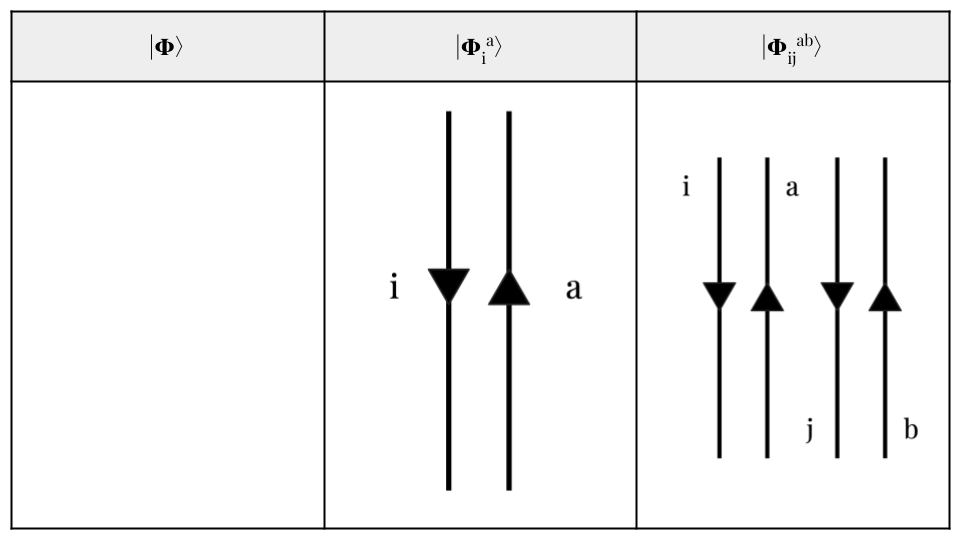
\includegraphics[scale=0.25]{Images/Chapter2/Diagrams_1.png}
    \caption{Diagrammatic representations for the Fermi vacuum state, the one-particle one-hole excited state, and the two-particle two-hole excited state.}
    \label{fig:diagrams1}
\end{figure}

Representing the excited states as creation and annihilation operators acting on the Fermi vacuum state is also possible. Remember that the one-particle one-hole excited state can be written as $|\Phi_i^a\rangle = a_a^\dagger a_i|\Phi_0\rangle$ where $a^\dagger$ is a fermionic creation operator and $a$ is the fermionic creation operator. This means that the two-particle two-hole excited state can be written as $|\Phi_{ij}^{ab}\rangle = a^\dagger_aa^\dagger_ba_ia_j|\Phi_0\rangle$.

The state $a_a^\dagger a_i|\Phi_0\rangle$ can be represented the same way as $|\Phi_i^a\rangle$, but with two horizontal lines at the bottom to represent the Fermi vacuum state. To represent the bra of this state ($\langle \Phi_i^a| = \langle \Phi_0|a^\dagger)_ia_a$ is represented in the same way, but the vertical lines representing the Fermi vacuum state are moved to the top. The two-particle two-hole excited state is represented similarly. These diagrams are shown in Fig. \ref{fig:diagrams2}.  Note that there is some ambiguity in the representation of $|\Phi_{ij}^{ab}\rangle$ in this representation, it could also represent $|\Phi_{ij}^{ba}\rangle$.

\begin{figure}
    \centering
    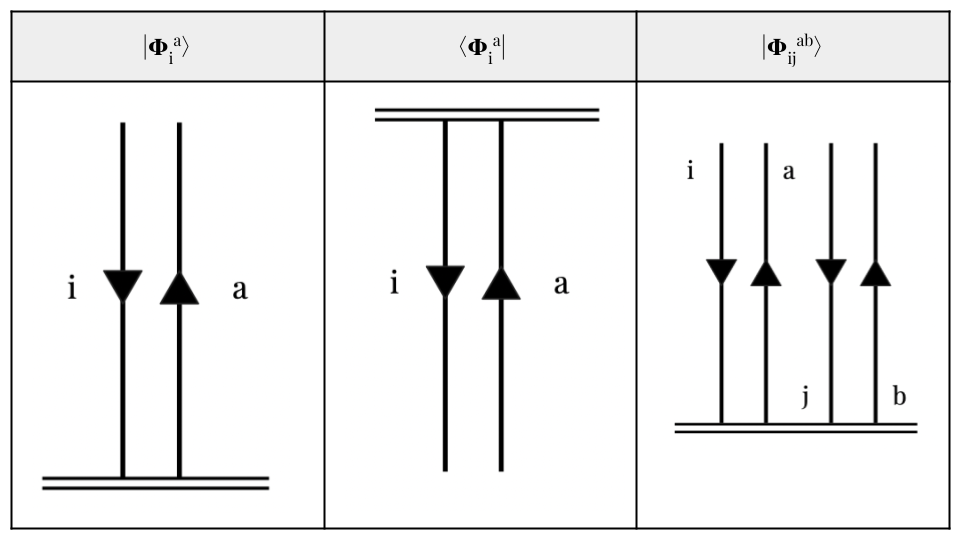
\includegraphics[scale=0.25]{Images/Chapter2/Diagrams_2.png}
    \caption{Diagrammatic representations for the one-particle one-hole and two-particle two-hole excited states written as annihilation and creation operators applied to the Fermi vacuum state.}
    \label{fig:diagrams2}
\end{figure}

%% Basic operator notation
Now that we have the diagrammatic notation for the various states, we can define a notation for the various operators. Here we will explicitly define the one-body and two-body operators in diagrammatic notation, but the form of the higher-order operators will follow the same patterns.

We can define a generic one-body operator as:

\begin{equation}
    \hat{O}_1 = \sum_{pq}\langle p | \hat{o}_1 | q \rangle \{a^\dagger_pa_q\},    
\end{equation}

where p and q can be occupied or unoccupied states, this one-body operator can be represented with either diagram in Fig. \ref{fig:one_body_generic}. The horizontal orientation of the lines does not matter so the lines can be in the purely vertical orientation, as in the left diagram, or they can be slanted, as in the right diagram. Since the lines in neither diagram of Fig. \ref{fig:one_body_generic} have directional arrows, the lines are represented by indices p and q.

\begin{figure}
    \centering
    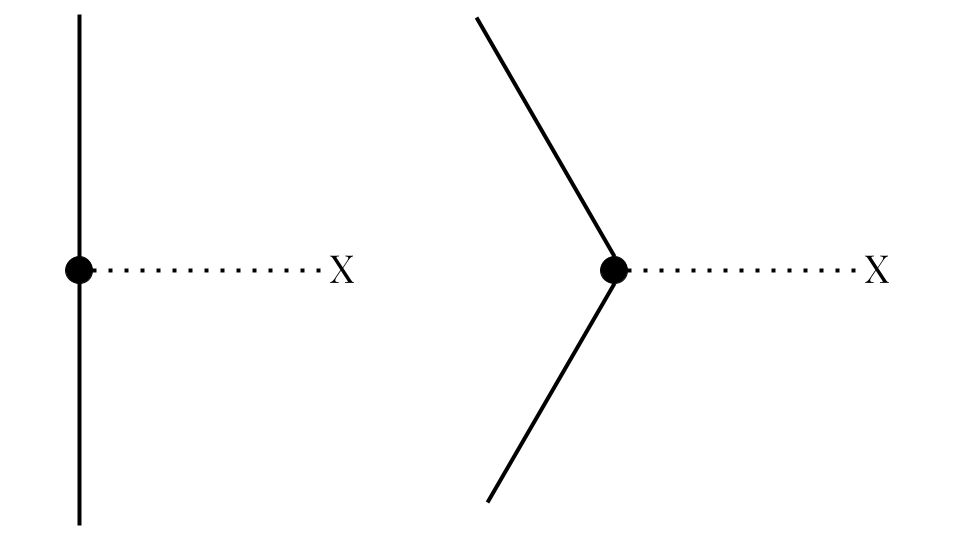
\includegraphics[scale=0.25]{Images/Chapter2/one_body_generic.png}
    \caption{A generic representation of the one body operator. The orientation of the lines does not matter, so the diagram can be represented with both lines being entirely vertical or with the lines being slanted. Since these lines do not have arrows, they represent generic single-particle states that could be occupied or unoccupied in the Fermi vacuum state.}
    \label{fig:one_body_generic}
\end{figure}

When creating the specific diagrams for the one-body operator, there are four options, as shown in Fig. \ref{fig:one_body_specific}.  There is one diagram where both indices are from states that are unoccupied in the Fermi vacuum state, which is represented by the top left diagram and equation form as:

\begin{equation}
    \sum_{ab} \langle a | \hat{o}_1 | b \rangle \{a^\dagger_aa_b\}.
\end{equation}

One diagram also results from having both states taken from the states occupied in the Fermi vacuum state. This is the diagram shown in the top right of Fig. \ref{fig:one_body_specific} and is represented in equation form as: 

\begin{equation}
    \sum_{ij} \langle i | \hat{o}_1 | j \rangle \{a^\dagger_ia_j\}.
\end{equation}

Finally, two diagrams can be created: one state is drawn from the occupied states and one from the unoccupied states. These are shown in the bottom row of Fig. \ref{fig:one_body_specific}. The bottom left diagram is represented in equation form:

\begin{equation}
    \sum_{ia} \langle a | \hat{o}_1 | i \rangle \{a^\dagger_aa_i\},
\end{equation}

the bottom right diagram in equation form is:

\begin{equation}
    \sum_{ia} \langle i | \hat{o}_1 | a \rangle \{a^\dagger_ia_a\}.
\end{equation}

\begin{figure}
    \centering
    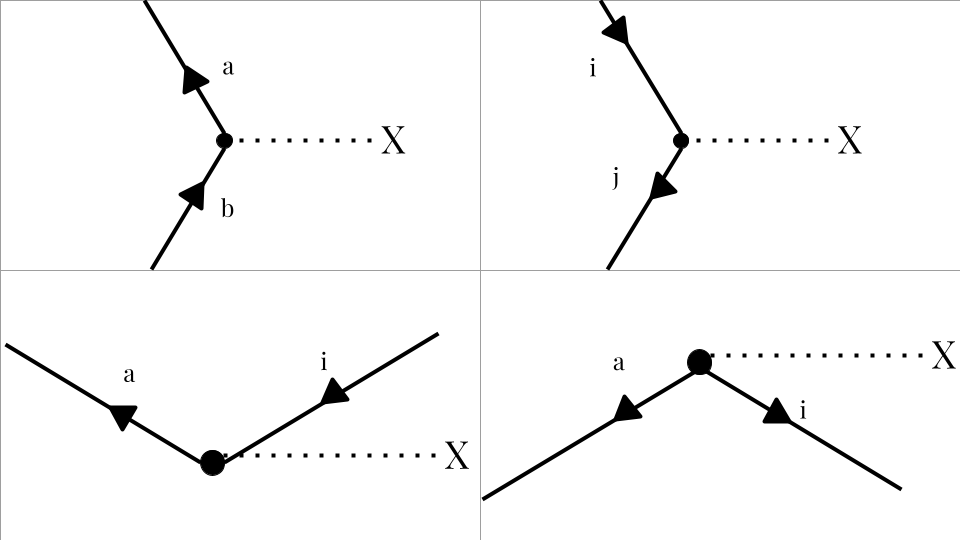
\includegraphics[scale=0.5]{Images/Chapter2/one_body_specific.png}
    \caption{The specific diagrams for the one-body operator, with the top left diagram for two unoccupied states, the top right diagram for two unoccupied states, and the bottom two diagrams containing one occupied and one unoccupied state.}
    \label{fig:one_body_specific}
\end{figure}

In the diagrams, the summation of the indices is implied using Einstein notation. In general, when creating diagrams from an equation, the index in the bra of the matrix element will exit the interaction vertex, and the index in the ket will be the line that enters the interaction vertex: $\langle left\ line | \hat{o}_1 | right\ line \rangle$.  

Finally, in this section, we can move onto the diagrammatic representation of a generic two-body operator, which we can represent in equation form as:

\begin{equation}
    \hat{O}_2 = \sum_{pqrs}\langle pq | \hat{o}_2 | rs \rangle \{a^\dagger_pa^\dagger_qa_sa_r\}.
\end{equation}

The generic two-body diagram can be described in Fig. \ref{fig:two_body_general}, and the nine specific two-body diagrams can be found in Fig. \ref{fig:two_body_specific}.

\begin{figure}
    \centering
    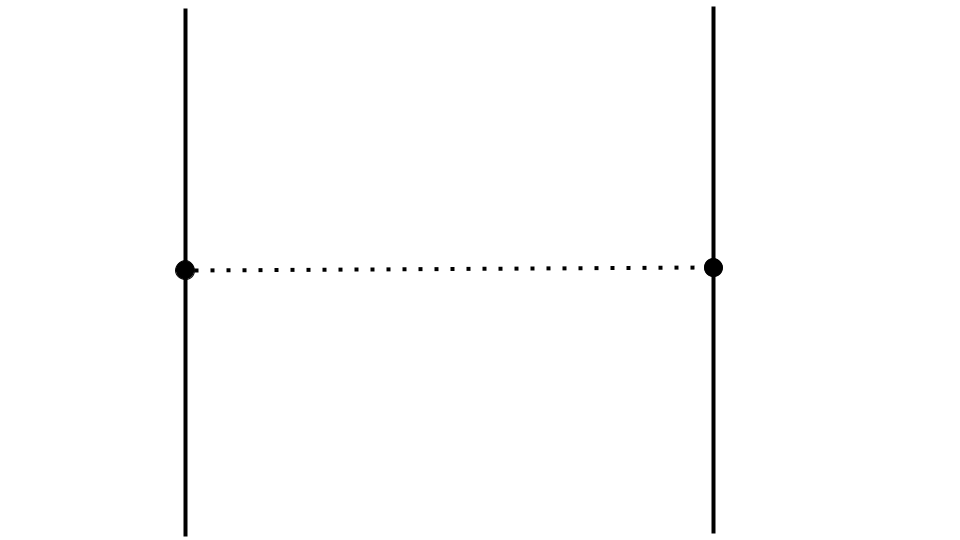
\includegraphics[scale=0.25]{Images/Chapter2/two_body_generic.png}
    \caption{The general diagram for a two-body interaction.}
    \label{fig:two_body_general}
\end{figure}

\begin{figure}
    \centering
    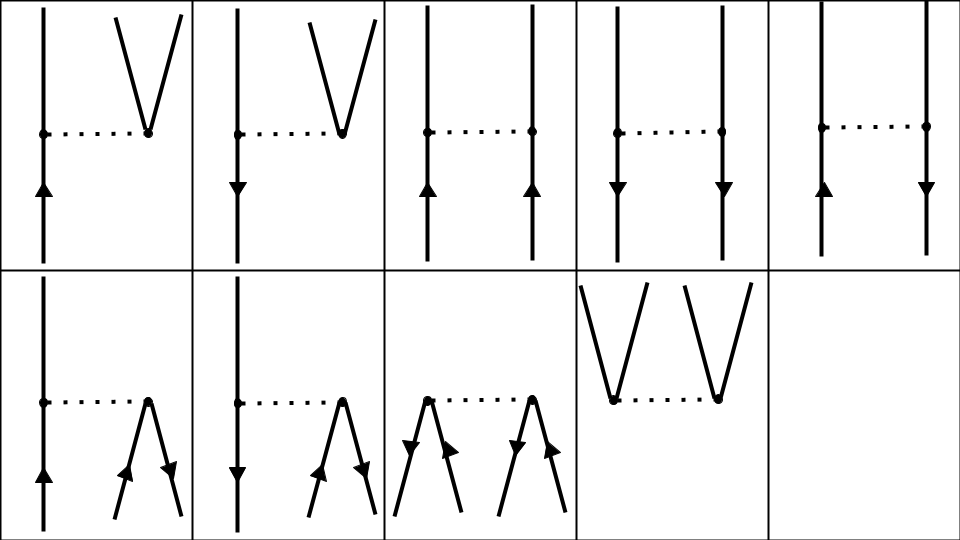
\includegraphics[scale=0.25]{Images/Chapter2/two_body_specific.png}
    \caption{The nine specific diagrams for a two-body interaction.}
    \label{fig:two_body_specific}
\end{figure}

From these examples, we can begin to create a set of rules for creating these diagrams and converting them to algebraic expressions:

\begin{enumerate}
    \item Lines representing occupied states in the Fermi vacuum are labeled with indices like $i$, $j$, $k$, ... and point downwards. Lines representing unoccupied states in the Fermi vacuum are labeled with indices $a$, $b$, $c$, ... and point upwards. Finally, lines that could represent either type of state are labeled with indices $p$, $q$, $r$, ... and have no directional arrows.
    \item The horizontal arrangement and spacing of the diagrams do not matter.
    \item Lines that represent the bra of the interaction matrix element leave an interaction vertex and are called external lines.
    \item Lines that represent the ket of the interaction matrix element enter an interaction vertex and are called internal lines.
    \item Every one body interaction vertex represents the factor $\langle out | \hat{o}_1 | in \rangle$.
    \item Every two-body interaction vertex represents the factor $\langle left-out\ right-out | \hat{o}_2 | left-in\ right-in \rangle$.
    \item If two lines start and end in the exact location, they are considered equivalent. Each set of equivalent lines in a diagram represents a factor of 1/2.
    \item The sign of a diagram is calculated using $(-1)^{(n_{occ} + l)}$, where $n_{occ}$ are the number of lines representing states that are occupied in the Fermi vacuum state and l is the number of loops in the diagram.
    \item Each pair of unique external lines (i.e., the bras of the interactions) that are not connected to the same interaction picks up a permutation factor.
\end{enumerate}
    \section{Conclusion}
        %%% THESIS CONCLUSIONS %%%

% SRE as a valid extrapolation method
The sequential regression extrapolation (SRE) method developed here based on Bayesian regression algorithms is an accurate and valuable extrapolator for removing basis incompleteness errors from coupled cluster calculations of infinite matter systems. Furthermore, when the infinite matter system needs to be taken to the thermodynamic limit, it is possible to use SRE to perform this task. Since the SRE algorithm uses training data taken from calculations at small numbers of single-particle states to predict the correlation energy at many single-particle states, the SRE algorithm can offer significant time savings over performing fully converged correlation energy calculations. As shown in this thesis, using the SRE algorithm to save over 100 node hours in the calculations of just one correlation energy is possible. Furthermore, this huge time savings does come with a loss in the accuracy of performing the whole savings. However, the average percent error between the SRE prediction and the fully calculated result was typically less than 1$\%$, making it quite a slight difference compared to the large amount of computational time that has been saved.

% From the CCD vs. CCDT side
Furthermore, besides developing the SRE method, we also compared different methods of performing coupled cluster calculations of systems of infinite nuclear matter. First, we compared the results from two different interactions: the Minnesota potential, a toy interaction, and chiral NNLO potentials, which are much more realistic. By comparing these two, we learned that they differ quite significantly around densities of infinite nuclear matter that are similar to nuclear densities and that calculations containing NNLO potentials do take much longer to compute compared to a Minnesota potential applied to the same system. Furthermore, we could also compare the difference between the coupled cluster approximations CCD, CCDT-1, and CCD(T) on calculations of infinite matter systems. We found that the triples approximations give significant results when compared to the CCD approximation, so they are worth performing even though they provide an increase in computational time.

%% SIZE OF MACHINE LEARNING SYSTEM
Though it has been mentioned throughout this thesis, it is essential to emphasize the size of the training data sets used in this work. This work's most extensive training data set used only 16 training points, and the smallest training set used only 3 points. Some areas of physics could be faster to adopt machine learning because of the vast amount of training data that some machine learning algorithms require. However, this work has shown that accurate machine learning predictions can be made with very few training points, thus encouraging using machine learning as a tool in fields with small data sets.

%%% FUTURE WORKS %%%

\subsection*{Possible Future Works}
% Full triples and different proton fractions
A few notable future works stem directly from the work presented here. First, while we showed results from both the CCD< CCDT-1, and CCD(T) approximations, we did not have the capabilities to produce coupled cluster correlation energies using a complete CCDT calculation. This is mainly due to the high computational costs of a complete triple calculation ($O(M^8)$), but advancements, such as those made in Refs. Furthermore, ADD REFERENCES HERE are making this a much more achievable goal for the near future.

Additionally, while we only looked at pure neutron matter and symmetric nuclear matter here, there are other proton fractions of interest. If we want to model the equation of the state of nuclear matter thoroughly, then we need to be able to accurately predict the properties of neutron matter at proton fractions beyond just 0.0 and 0.5.

% PARAGRAPH ABOUT NOT BEING LIMITED TO INFINITE SYSTEMS
While truncating the number of particles in a calculation is limited to infinite matter and other large systems, truncations occur in every \textit{ab initio} many-body calculation. Basis truncation is especially common and occurs in almost every calculation except some simple toy models. The last part of this thesis will be dedicated to exploring some possible future applications of the SRE methodology which has been developed.

% PARAGRAPH ABOUT CC CALCULATIONS OF THE NUCLEUS
An extension of the work presented in this thesis is to apply the SRE method to remove basis incompleteness errors from coupled cluster calculations of nuclei. Though nuclei are finite systems and the number of nucleons in the system generally does not need to be truncated, the number of single-particle states is still truncated, leading to a need to extrapolate to an infinite model space \cite{Ref6}. This is especially true for heavy nuclei and nuclei that are weakly bound \cite{Ref6}. There are methods to perform these extrapolations on nuclei calculations, but when using the harmonic oscillator basis, which mixes the ultraviolet and infrared cutoffs, these extrapolation methods can fail \cite{Ref6}. Machine learning has been used to perform similar extrapolations (see Ref. \cite{Ref6}, \cite{Ref22}, \cite{Ref23}, for example), but these were performed with neural networks and thus incurred all of the problems that were experienced with neural networks in this thesis.

%% MBPT CALCULATIONS AND HIGHER ORDERS
Additionally, the SRE method has no reason to be restricted to only predicting CC energies using MBPT2 energies. Extending the SRE method to other many-body methods should also be possible. 

% PARAGRAPH ABOUT FCI
One of the most accurate yet restricted \textit{ab initio} many-body methods is full configuration interaction theory (FCI), which uses a variationally optimized linear combination of the full set of Slater determinants. FCI is used in nuclear physics and electronic-structure theory, but its complexity limits it to only the smallest of systems. The ground state energy, which FCI finds, is the lowest (variationally) and most accurate that can be achieved. If an infinite single particle basis is used, FCI produces the solutions to the Schr\"{o}dinger equation. However, due to computational limitations, FCI calculations must be performed with a finite basis, meaning they will fail to retrieve the total energy \cite{Ref1}. However, it is possible that SRE could be applied to FCI calculations using, for example, Hartree Fock calculations as the "fast method" to quickly and accurately extrapolate FCI results to the infinite basis limit, thus recovering the Schr\"{o}dinger equation results.

 % APPLICATIONS OUTSIDE OF NUCLEAR PHYSICS
While most of this thesis, except for the sections on the electron gas, have been devoted to nuclear physics applications, \textit{ab initio} many-body methods occur in many other fields besides nuclear physics. For example, coupled cluster theory, and other many-body methods, are prevalent in other fields of physics and quantum chemistry. Therefore, the development of the SRE method should improve calculations outside of the realm in which it was developed.

    %%%%%%%%%%%%%%%%%%%%%%%%%%%%%%
    %% Full Configuration Interaction Theory
    %%%%%%%%%%%%%%%%%%%%%%%%%%%%%%
    %\section{Full Configuration Interaction Theory}
    %    \input{Text/Chapter2/FCI.tex}


%%%%%%%%%%%%%%%%%%%%%%%%%%%%%%
%% CHAPTER: MBPT AND CC
%%%%%%%%%%%%%%%%%%%%%%%%%%%%%%
\chapter{Many-Body Theories}
    
    %%%%%%%%%%%%%%%%%%%%%%%%%%%%%%
    %% INTRODUCTION
    %%%%%%%%%%%%%%%%%%%%%%%%%%%%%%
    \section{Introduction}
        \chapter*{Introduction}

%VMC methods pose a very attractive alternative to other more complex ways of finding the ground state energies of simple atoms and molecules, like configuration-interaction calculations. The price to be paid in exchange for this simplicity is the sensitivity to the trial wave functions that are used, a VMC algorithm is very sensitive to how these are constructed, so they are one of the most important aspects to be considered (in this work, given the simple nature of the atoms which we will be working with, it's not so important to worry about the quality of the trial wave functions because very simple and basic ones are more than enough to reproduce the actual results). It shouldn't be forgotten that it is a variational method, and this implies that finding the optimal set of variational parameters is going to be the most important part of the calculation itself because it would create a lot of problems if the search range for the parameters was illy defined and not close enough to the variational minimum, namely, the results would have a poor quality in this case. This means that the parameters need to be chosen very carefully, or a recursive search with decreasingly coarse spacing in the space of variational parameters is required if there is no deep knowledge about the system in question.

%Instead of evaluating a very complex multidimensional integral to compute the expectation value of an operator, like the hamiltonian in this case, a VMC calculation exploits the fact that the majority of the configuration space where the wave function belongs can be regarded as much less important than other parts, the values of the wave function are too small there and can be mostly ignored during the integration of the algorithm. To capitalize this, the Metropolis algorithm is added to the VMC method, as well as importance sampling and Gaussian Type Orbitals.

%\todo{motivasjon (QD i 2D og 3D + atomer -> fleksibel kode)}
%\subsubsection{Introducing the problem and the flexible solver}
Quantum mechanical systems are complex. As such creating a specific
program for each specific system is not a viable method of studying a
range of systems. We need to generalize. A generalized solver for
quantum mechanical systems must be written without any constraints to
specific properties any system may have. To achieve such a feat the
program is best implemented by the use of object orientation, creating
an easily expandable solver to which simple or complex systems may be
added. In this thesis the aim is to write a generalized variational
Monte Carlo solver which, by using object orientation, may handle a
wide range of quantum mechanical systems, such as confined electrons
in so-called quantum dots, atoms, and molecules.

%\subsubsection{Further introduction to the solver, the trial function, the slater determinant}
The variational Monte Carlo method poses an attractive way to solve
quantum mechanichal systems, compared to other more complex methods,
while also taking correlation factors into account, as opposed to the
Hartree-Fock method. The attractiveness of the variational Monte Carlo
method lies in the way it solves the multi-dimensional integrals
arising in the many-body quantum mechanical problem, which, as the
name implies, is by using the Monte Carlo method. In this thesis a
single so-called Slater determinant is used as an ansatz for the trial
wave function. This simplicity makes it easy to implement an efficient
and flexible program. It is however a compromise, yielding less
accurate results, but nevertheless good enough to study a variety of
systems.

%\subsubsection{Introducing the QD problem in 2 and 3 dimensions, and atoms. Tie to use of flexible code}
The solver presented in this thesis was initially made to solve simple
atomic systems, as a reference, and thereby expanding to molecules. To further
demonstrate the flexibility of the program, quantum dots are studied
in two and three dimensions. The reason for choosing quantum dots to
be studied is their simple structure, yet multitude of practical uses.


%\todo{hva jeg har gjort}
%\subsubsection{Introduce implementation of the code}


%\subsubsection{Short description of various tests done with QD and atoms}
The aim in this thesis is to demonstrate the flexibility of the
program by studying the system like atomic helium, beryllium and neon,
the helium and beryllium molecules, benchmarking ground state energies
against existing references, and studying their one-body densities. Furthermore
quantum dots consisting of up to 56 electrons will be studied in a
similar manner, and their frequency will be varied.  With a lower
frequency the quantum dots will implicity have a higher correlation,
and studying correlations are of great importance when using more
elaborate methods than for example the simple Hartree-Fock method.

Ground states of atoms and molecules are compared to experimental
results, which should be close to the exact results, offering a good
test of the accuracy of the variational Monte Carlo method and the
solver created. Because of the popularity of quantum dots several
master students have studied them, each with different methods. This
provides a wide range of references to which ground state energies may
be compared, which should give further insight to the accuracy of the
solver.

%\todo{oppgavens struktur}
%\subsubsection{Chapter by chapter}
The thesis is structured in two parts: a theory part, and a results part. A brief description of the chapters is given below.
\begin{itemize}
	\item In the first chapter a brief introduction to scientific computing is given. In it different types of programming languages will be described, and we will give an introduction to object-oriented programming. This is important because object-oriented programming is used to create a generalized solver. A summary of message passing interface, used to parallelize the computations, is also given.  
	\item The second chapter aims to give an overview of a more basic solution method, the Hartree-Fock method. It also describes other methods derived from the Hartree-Fock method, so-called post Hartree-Fock methods. The Hartree-Fock method can be used as a convenient test for a more simplified variational Monte Carlo program, and some of the post Hartree-Fock methods are used in computations of references when ground state energies computed by the solver is benchmarked.
	\item Next the variational Monte Carlo method is explained with details around ways of optimization, like the Metropolis algorithm and importance sampling. Details about how to calculate the Slater determinant efficiently and other measures to further optimize the solver are also given. Then the process of blocking to get an accurate estimate of the error is explained.
	\item In the fourth chapter the modelled systems are described. How quantum dots are modelled in two and three dimensions is described, then a brief descrition of how each of the atomic systems are modelled is given. A way to replace the Slater type orbitals with gaussian type orbitals is also described.
	\item In the final chapter of the first part we look at how the solver is structured, and how the variational Monte Carlo method is implemented using object-orientation.
	\item With the theory in place we look at the results from calculations with the variational Monte Carlo solver created. The program is benchmarked to test the optimizations and also to see how well it scales with an increasing number of processors used. The systems are benchmarked against reference ground state energies, and one-body densities are calculated, which can give insight into the structure of the systems. 
	\item Finally a conclusion is given with final remarks.
\end{itemize}


%`God does not play dice' Einstein said \todo{ref}, refuting the theory that quantum mechanical systems are governed by probability. However, as it turns out, we may, to solve them.


    %%%%%%%%%%%%%%%%%%%%%%%%%%%%%%
    %% Hartree-Fock Theory
    %%%%%%%%%%%%%%%%%%%%%%%%%%%%%%
    \section{Hartree-Fock Theory}
        The first many-body method we will explore in this chapter is the Hartree-Fock theory (HF) \cite{Ref161, Ref162}. HF, one of the earliest many-body methods, is an iterative algorithm that can be used to find the ground state of a system given its Hamiltonian \cite{Ref5}. As an independent-particle model, Hartree-Fock Theory begins with the Slater determinant, defined in Section 2.2 and rewritten here:

\begin{equation}
    \Phi = \frac{1}{N} \begin{vmatrix}
        \psi_1(\vec{x}_1) & \psi_2(\vec{x}_1) & . & . & . & \psi_N(\vec{x}_1) \\
        \psi_1(\vec{x}_2) & \psi_2(\vec{x}_2) & . & . & . & \psi_N(\vec{x}_2) \\
        . & . & . & . & . & . \\
        . & . & . & . & . & . \\
        . & . & . & . & . & . \\
        \psi_1(\vec{x}_\nu) & \psi_2(\vec{x}_\nu) & . & . & . & \psi_N(\vec{x}_\nu) \\
    \end{vmatrix},
\end{equation}

where $\Phi$ is the many-body wavefunction and $\psi_n(\vec{r}_m)$ is the single-particle wavefunction of the $m$-th particle with spatial and spin coordinates described by $\vec{r}_m$. Hartree-Fock Theory uses an iterative algorithm to vary the single-particle wavefunctions, $\psi$ such that the energy of the entire many-body wavefunction, represented by the Slater determinant, is minimized \cite{Ref21}. This minimization can be achieved by solving eigenvalue problems for all single-particle wavefunctions. All of the eigenvalue equations are coupled and have the form:

\begin{equation}
    \hat{f} \psi_i = \epsilon_i \psi_i,
\end{equation}

where $\epsilon_i$ is the single-particle energy and $\hat{f}$ is the single-particle Fock operator.  The single-particle Fock operator, which depends on all of the single-particle wavefunctions, has the following matrix elements:

\begin{equation}
    \langle p | \hat{f} | q \rangle = \langle p | \hat{t} | q \rangle + \sum_i \langle pi | \hat{v}_2 | qi \rangle_{A},
\end{equation}

where $\hat{t}$ is the single-particle kinetic energy operator and $\hat{v}_2$ is the interaction between two particles \cite{Ref4}.  It is important to note that for nuclear problems, interactions beyond the two-body level contribute significantly to the total interaction. We can also define the many-body Fock operator, $\hat{F}$, as:

\begin{equation}
    \hat{F} = \sum_{pq} \langle p | \hat{f} | q \rangle a^\dagger_p a_q.
\end{equation}

For many systems, the solution provided by HF provides an excellent initial approximation for the ground state energy and its corresponding many-body wavefunction. HF can recover approximately 99$\%$ of the ground state energy and approximately 95$\%$ of the corresponding wavefunction for electronic systems \cite{Ref4, Ref21}. However, since HF is an independent particle model, the missing energy comes from the interaction between particles, and therefore this energy must be recovered as well. The need to recover the energy from the interactions between particles, known as the correlation energy, has led to the development of more advanced many-body methods. This chapter will develop two of these, many-body perturbation theory and coupled cluster theory.

    %%%%%%%%%%%%%%%%%%%%%%%%%%%%%%
    %% MBPT
    %%%%%%%%%%%%%%%%%%%%%%%%%%%%%%
    \section{Many-Body Perturbation Theory}
        By this point, it has been well established that finding the energy of a many-body system is done by solving the following eigenvalue problem where $|\Psi \rangle$ is a many-body wavefunction:

\begin{equation}
     \hat{H} | \Psi \rangle = E | \Psi \rangle \longrightarrow \langle \hat{H} | \Psi \rangle = E.
\end{equation}

However, this problem can only be solved fully for a few uninteresting systems. Therefore, we have developed our first many-body method, HF theory, capable of finding approximately the energy of a many-body system. However, HF is an independent particle model, and we also wish to include the interactions between the particles in the energy. Thus, we will start by developing many-body perturbation theory (MBPT), a post-Hartree-Fock method, so called because it starts with the Hartree-Fock energy but then adds a correction to account for the interactions between the particles \cite{Ref21, Ref163, Ref164, Ref165}.

Many-body perturbation theory assumes that the Hamiltonian can be split into two pieces, a non-interacting component, $\hat{H}_0$, and an interacting component, $\hat{H}_I$. The interacting component is a small perturbation away from the non-interacting component, thus the method's name. Thus, we have:

\begin{equation}
    \hat{H} = \hat{H}_0 + \hat{H}_I.
\end{equation}

From this definition of the Hamiltonian, we can split the energy of the many-body system into two components: a reference energy, $E_0$, and a correlation energy, $\Delta E_{MBPT}$, leading to:

\begin{equation}
     E = E_{Ref} + \Delta E_{MBPT}.
\end{equation}

The reference energy is defined using the total Hamiltonian and the Fermi vacuum state, $|\Phi_0\rangle$ and the total Hamiltonian as:

\begin{equation}
    E_{Ref} = \langle \Phi_0 | \hat{H} | \Phi_0 \rangle.
\end{equation}

In practice, the reference energy is, in fact, the Hartree-Fock energy, assuming we are using a Fock basis, which we will be using for every calculation in this thesis. Thus the correlation energy is an additional term to the MBPT energy compared to the HF energy.

Now we can define the MBPT correlation energy as the matrix elements formed when the interacting component of the Hamiltonian is applied to a many-body wavefunction as the ket and the Fermi vacuum as the bra, giving:

\begin{equation}
    \Delta E_{MBPT} = \langle \Phi_0 | \hat{H}_I | \Psi \rangle.
\end{equation}

However, solving equation is no simpler than solving the original eigenvalue problem. Thus we will rephrase the MBPT correlation energy as:

\begin{equation} \label{correlation}
    \Delta E_{MBPT} = \sum_{i=1}^\infty \Delta E^{(i)},
\end{equation}

where $\Delta E^{(i)}$ is the i-th order correction to the MBPT correlation energy. We can define the form of the first two corrections as follows. The first order correction to the MBPT energy is:

\begin{equation}
    \Delta E^{(1)} = \langle \Phi_0 | \hat{H}_I | \Psi_0 \rangle.
\end{equation}

The second order correction to the MBPT energy is: 

\begin{equation}
    \Delta E^{(2)} = \frac{1}{4} \sum_{ijab} \frac{\langle ij | \hat{V}_2 | ab \rangle \langle ab | \hat{v}_2 | ij \rangle}{(\epsilon_i + \epsilon_j) - (\epsilon_a + \epsilon_b)}
\end{equation}

Theoretically, there are infinite corrections to the MBPT correlation energy. In practice, we cannot compute infinite corrections to the MBPT energy, and we must truncate Eq. \ref{correlation} to a finite number of terms. However, the form of the correlation energy provides a convenient truncation scheme. The MBPT truncation MBPT1 (many-body perturbation theory to the first order) uses the approximation $\Delta E_{MBPT} \approx \Delta E^{(1)}$, the MBPT truncation scheme MBPT2 (many-body perturbation theory to the second order) uses the approximation $\Delta E_{MBPT} \approx \Delta E^{(1)} + \Delta E^{(2)}$, and so on. This thesis will primarily focus on MBPT2 as the leading MBPT approximation used in these calculations. Any MBPT results presented here will only include one-body and two-body interactions.    

    %%%%%%%%%%%%%%%%%%%%%%%%%%%%%%
    %% Coupled Cluster Theory
    %%%%%%%%%%%%%%%%%%%%%%%%%%%%%%
    \section{Coupled Cluster Theory}
        %%%%%%%%%%%%%%%%%%%%%%%%%%%%%%
        %% introduction to the method
        %%%%%%%%%%%%%%%%%%%%%%%%%%%%%%
        \subsection{Introduction to the Method}
            Coupled cluster theory (CC), initially developed in nuclear physics (for its development, see Ref. \cite{Ref153, Ref152}, and for its resurgence in nuclear physics, see Ref. \cite{Ref147, Ref68, Ref16, Ref154, Ref148}), has long been the goal standard for quantum chemistry calculations (\cite{Ref149}). CC provides a method to systematically include complicated interactions beyond the mean field, is non-perturbative, size extensive, non-variational, and is widely used for performing calculations on strongly correlated systems \cite{Ref8}. Being size-extensive is important for CC to be applied to large systems. Computationally, CC scales polynomially with respect to the number of occupied and unoccupied states in the system, making it an efficient many-body method for small to medium-sized systems but relatively slow for large systems.  Compared to MBPT, CC is a more accurate method but also incurs more extensive computational run times.

In quantum chemistry and electronic structure, CC is considered the "gold-standard" many-body method but also can be too computationally expensive for some applications, especially for studies of larger molecules \cite{Ref7}. However, quantum chemists have made great strides in accelerating coupled cluster calculations of electronic systems through various methods, including truncations, which will be discussed in a few sections. For interesting applications of coupled cluster theory in quantum chemistry, see, for example, Ref. \cite{Ref140, Ref141, Ref149, Ref142,Ref143,Ref145,Ref150,Ref155,Ref7,Ref67,Ref72,Ref74}.

In CC, we can represent the $N$-Fermion wavefunction ($|\Psi\rangle$) using the so called exponential ansatz:

\begin{equation} \label{cc_ansatz}
    |\Psi \rangle = e^{\hat{T}} |\Phi_0 \rangle.
\end{equation}

In the above equation, $|\Phi_0\rangle$ is the Fermi vacuum state where the $N$ particles in the system occupy the $N$ lowest energy states. $\hat{T}$ is known as the correlation or the cluster operator, and it is the sum of $N$ operators, where $N$ is the number of particles in the system \cite{Ref8, Ref7}, and can be written as:

\begin{equation} \label{cluster}
    \hat{T} = \sum_{i=1}^N \hat{T}_m.
\end{equation}

Each $\hat{T}_m$ operator in Eq. \ref{cluster} represents the m-particle m-hole excitation operator, which has the below form \cite{Ref8,Ref7}.

%% ADD CHANGE IN NOTATION FROM |p> to |kp>%%%%%%%

\begin{equation} \label{m_particle_m_hole}
    \hat{T}_m = (\frac{1}{m!})^2 \sum_{i_1...i_m\\
                  a_1...a_m} t^{a_1...a_m}_{i_1...i_m} a^\dagger_{a_1}...a^\dagger_{a_m}a_{i_m}...a_{i_1}
\end{equation}

Single-particle states with labels $i_n$ correspond to states occupied in the Fermi vacuum state, and single-particle states with the labels $a_n$ correspond to states unoccupied in the Fermi vacuum state. The operator $a^\dagger$ is the Fermion creation operator, and the operator $a$ is the Fermion annihilation operator (both are defined in Chapter 2). The coefficients $t$ are called T-amplitudes, and they are determined through a complex set of non-linear equations:

\begin{equation} \label{CC_amplitude}
    \langle \Phi^{a_1, a_2, ...,a_k}_{i_1, i_2, ...,i_k} | e^{-\hat{T}}\hat{H}e^{\hat{T}} | \Phi_0 \rangle = 0,
\end{equation}

where the index $k$ = 1, 2, ..., A \cite{Ref8}. When $k$ = 1, the 1-particle 1-hole excitation operator is recovered ($\hat{T}_1$), when $k$ = 2 the 2-particle 2-hole excitation operator is recovered ($\hat{T}_2$), and so on. Therefore, amplitude equations must be solved for untruncated coupled-cluster theory to fully derive the cluster operator for an $N$-body system. If coupled cluster equations are solved with the untruncated cluster operator, they arrive as the same result as Schr\"{o}dinger's equation.

It is important to note that in Eq. \ref{CC_amplitude}, we have used a shorthand notation to refer to the bra vector, which is, in fact, a $k$-particle $k$-hole excitation of the Fermi vacuum state \cite{Ref8}. Written out fully in second quantization, we can define the $k$-particle $k$-hole excitation of the Fermi vacuum state as:

\begin{equation} \label{Fermi_excite}
    |\Phi^{a_1, a_2, ..., a_k}_{i_1, i_2, ..., i_k} \rangle = a^\dagger_{a_1} ... a^\dagger_{a_k}a_{i_k} ... a_{i_1}|\Phi_0\rangle,
\end{equation}

where $a^\dagger$ is the Fermion creation operator, and $a$ is the Fermion annihilation operator.

As a note on notation, the T-amplitudes, scalars that are calculated through determining the m-particle m-hole excitation operators, can be represented equivalently in the following two notations:

\begin{equation}
t^{a_1...a_m}_{i_1...i_m} = \langle a_1...a_m | \hat{t} | i_1...i_m \rangle.
\end{equation}

As an aside from the form of the CC wavefunction: 

\begin{equation} \label{cc_ansatz}
    |\Psi\rangle = e^{\hat{T}}|\Phi_0\rangle,
\end{equation}

one can use a Taylor expansion to expand the exponential function to obtain:

\begin{equation} \label{cc_ansatz}
    |\Psi\rangle = (1 + \hat{T} + \hat{T}^2/2! + \hat{T}^3/3! + ...)|\Phi_0\rangle.
\end{equation}

This expansion explains why some of the later CC approximations we will be looking at contain terms such as $\hat{T}_1$ and $\hat{T}_2$ but also $\hat{T}_1\hat{T}_2$ and $\hat{T}_1^3$.
        %%%%%%%%%%%%%%%%%%%%%%%%%%%%%%
        %% energy and correlation energy
        %%%%%%%%%%%%%%%%%%%%%%%%%%%%%%
        \subsection{Energy and Correlation Energy}
            Given an $N$-body many-body wavefunction, its energy can be determined by solving the eigenvalue problem that results from applying the Hamiltonian to the wavefunction (i.e., solving the time-independent Schr\"{o}dinger's equation) using:

\begin{equation} \label{schrodinger}
	\hat{H}|\Psi\rangle = E|\Psi\rangle.
\end{equation}

The above equation Eq. \ref{schrodinger} can give just the energy on the right-hand side of the left-hand side turned into a matrix element such that the equation now has the form:
 
\begin{equation} \label{matrix_element}
	\langle \Psi | \hat{H} | \Psi \rangle = E.
\end{equation}

Eq. \ref{matrix_element} has an implicit $\langle\Psi|\Psi\rangle = 1$ on the righthand side of the equation. From here, we can split the Hamiltonian into two pieces, the normal-ordered Hamiltonian and the vacuum expectation value:

\begin{equation}\label{split_H}
	\hat{H} = \hat{H}_N + E_0.
\end{equation}

where the vacuum expectation value $E_0$ is defined as:

\begin{equation}\label{vacuum_expectation}
	E_0 = \langle \Phi_0 | H | \Phi_0 \rangle.
\end{equation}

Combining Eqs. \ref{matrix_element} and \ref{split_H} yields:
\begin{equation}
	\langle \Psi | \hat{H}_N + E_0 | \Psi \rangle = E,
\end{equation}

which can be split up into the following two terms:

\begin{equation} \label{two_terms}
	\langle \Psi | \hat{H}_N | \Psi \rangle + \langle \Psi | E_0 | \Psi \rangle = E.
\end{equation}

Since $\langle\Psi | E_0 | \Psi\rangle = E_0\langle\Psi |\Psi\rangle = E_0$, then we can simplify Eq. \ref{two_terms} to:

\begin{equation}\label{two_terms_2}
	\langle \Psi | \hat{H}_N | \Psi \rangle + E_0 = E.
\end{equation}

From here, we can rewrite the coupled cluster exponential equation:

\begin{equation}
	e^{\hat{T}}|\Phi_0\rangle = |\Psi\rangle,
\end{equation}

which can be inserted into Eq. \ref{two_terms_2} to yield.

\begin{equation}
	\langle \Phi_0 | e^{-\hat{T}}\hat{H}_Ne^{\hat{T}} | \Phi_0 \rangle + E_0 = E.
\end{equation}

From here, we can define the similarity transformed normal ordered Hamiltonian to be:

\begin{equation}
	\bar{H}_N = e^{-\hat{T}}\hat{H}_Ne^{\hat{T}}, 
\end{equation}

which yields a final form of the energy equation:

\begin{equation}\label{energy_final}
	\langle \Phi_0 | \bar{H}_N | \Phi_0 \rangle + E_0 = E.
\end{equation}

In \ref{energy_final}, $E_0$ is known as the reference energy and (for this work) it is the Hartree-Fock energy. This makes coupled cluster a post-Hartree-Fock method, similar to MBPT. $\langle \Phi_0 | \bar{H}_N | \Phi_0 \rangle$ is the correlation energy or the coupled cluster correction to the Hartree-Fock energy. As a final definition for this section, the CC correlation energy will be represented as $\Delta E_{CC} = \langle \Phi_0 | \bar{H}_N | \Phi_0 \rangle$.

Much like MBPT, coupled cluster calculations will generally be reported in terms of the correlation energy instead of the total energy. Again, this is due to convention, as the correlation energy is the most important part of the energy calculation. Also note that for some systems (namely the infinite matter systems discussed in the next chapter), CC correlation energies are usually reported as the CC correlation energy per particle by convention such that systems with different numbers of particles can be compared.

The cluster operator $\hat{T}$ is undefined in the above equations. It is obtained by solving a set of coupled cluster amplitude equations set up in the previous section, of which there are $N$ sets of equations for an $N$ particle system. and the number of equations per set depends on the number of single particle states in the calculation. This system of equations is quite large even for relatively small systems and requires and iterative procedure to be solved. Defining the cluster operator (and, more specifically, the N t-amplitudes) is the most computationally extensive step when performing a CC energy calculation.
            
        %%%%%%%%%%%%%%%%%%%%%%%%%%%%%%
        %% computational methods and approximations
        %%%%%%%%%%%%%%%%%%%%%%%%%%%%%%
        \subsection{Computational Methods and Approximations} 
            For almost all CC calculations performed computationally, the cluster operator must be truncated \cite{Ref7}. Systems where CC calculations can be performed with the full cluster operator tend to be uninteresting toy models \cite{Ref8}. However, the form of the cluster operator provides a physically motivated method for truncation where all $m$-particle $m$-hole excitation operators over a certain level are set to zero. This approximation scheme is referred to as the SUB$_n$ approximation scheme \cite{Ref8}. There is also a convenient naming scheme when the cluster operator is truncated in this way. For example, if $\hat{T} \approx \hat{T}_1$, the approximation is called the coupled cluster single approximation (CCS), and if $\hat{T} \approx \hat{T}_1 + \hat{T}_2$ then we call this the coupled cluster singles and doubles approximation (CCSD), and if $\hat{T} \approx \hat{T}_1 + \hat{T}_2 + \hat{T}_3$ this leads to the coupled cluster singles, doubles, and triples approximation (CCSDT) \cite{Ref6}. Due to computational limitations, approximations over the triples level are rare, but have been performed on a limited set of systems \cite{Ref95}. For the infinite matter systems that are defined in the next chapter, the $\hat{T}_1$ operator gives no contribution to the energy so that we can simplify the above truncations: CCSD becomes CCD (coupled-cluster doubles) where $\hat{T} \approx \hat{T}_2$ and CCSDT becomes CCDT (coupled-cluster doubles and triples) where $\hat{T} \approx \hat{T}_2 + \hat{T}_3$. As the primary goal of this thesis is to use machine learning to extend the range of pre-existing coupled cluster methods instead of developing new methods or improving on existing methods, the explanations below are kept short and generally free of derivations. There have been many great works deriving the various coupled cluster methods in great detail, and we would like to point the readers to Refs. \cite{Ref21, Ref155, Ref149}, among others, for complete derivations of the methods introduced in this section.

As is expected, the higher the level of approximation, the more accurate the calculations but, the more extended run times. However, if having all $N$ terms in the cluster operator gives 100$\%$ of the energy of an $N$-particle system, then the CCSD approximation gives approximately 90$\%$ of the total energy, and CCSDT gives almost 99$\%$ of the total energy \cite{Ref21}. Each additional $m$-particle $m$-hole excitation operator does increase the accuracy of the energy calculation, but the improvements progressively decrease in size. Additionally, as expected, the computational time and resource requirements increase drastically as the order of the CC calculation increase. For example, the expected run time for a CCSD calculation is $O(M^6)$, where $M$ is the number of single-particle states. The expected run time for a CCSDT calculation is $O(M^8)$, and considering $M$ is likely to be 1,000 or higher for accurate calculations, this extra factor of $M^2$ represents a significant increase in run time. However, since we would like to achieve the accuracy of CCSDT, recovering 99$\%$ of the total energy, we can instead look at some approximative methods to the CCSDT approximation. These methods will not be as accurate as the CCSDT method, but they will be more accurate than the CCSD method as they contain some components from the $\hat{T}_3$ operator. Additionally, while these approximative triples methods will have a longer run time than a CCSD calculation, they will have much shorter run times than a complete CCSDT calculation, making the triples approximations a good balance of accuracy and run time.


\subsection{CCSDT Approximations}
There are two types of approximative triples calculations: non-iterative perturbative triples approximations, CCSD(T), and iterative CCSDT-n approximations.  The methods differ in their complexity and formulations, but give simular results and thus will be compared below.
    
	\subsubsection{Non-Iterative Triples Approximations}
    The perturbative triples approximation, CCSD(T), is a non-iterative triples approximation that is the gold standard for quantum chemistry applications \cite{Ref16}. The CCSD(T) method was developed in the late 1980s in the field of quantum chemistry \cite{Ref158}. The computational considerations for CCSD(T) have two components: an iterative component with a cost of $O(M^6)$ (the CCSD equations) and a non-iterative component with a cost of $O(M^7)$, making it faster than complete CCSDT calculations by a factor of M or greater. Since M can be over 1,000, this can represent a significant decrease in the run time for a calculation.
    
    We will start developing the CCSD(T) equations by defining the following two permutation operators:
    \begin{equation}
        \hat{P}(a/bc) = 1 - \hat{P}_{ab} - \hat{P}_{ac},
    \end{equation}

    and:

    \begin{equation}
        \hat{P}(a/bc | k/ij) = \hat{P}(a/bc) \hat{P}(k/ij),
    \end{equation}

    where $\hat{P}_{pq}$ is the permutation between states $p$ and $q$.  Next we can define an equation through which the $\hat{T}_3$ amplitudes can be defined from the $\hat{T}_2$ amplitudes:

    \begin{equation}\label{triples_amps}
        \epsilon_{ijk}^{abc}t_{ijk}^{abc} = \hat{P}(a/bc | k/ij) \sum_d \langle bc | \hat{v}_2 | dk \rangle t_{ij}^{ad} = \hat{P}(c/ab|i/jk)\sum_l \rangle lc | \hat{v}_2 | jk \rangle t_{il}^{ab},
    \end{equation}

    where:

    \begin{equation} \label{t3_from_t2}
         \epsilon_{ijk}^{abc} = (\epsilon_i + \epsilon_j \epsilon_k) - (\epsilon_a + \epsilon_b + \epsilon_c).
    \end{equation}

    Eq. \ref{triples_amps} defines the leading order (i.e., the second-order) terms in the full CCSDT triples equations. This equation will be used here to define the CCSD(T) method and in the next section to define the CCSDT-1a method. Next we can define $E_T^{(4)}$, the triples-excitation contributions to the MBPT4 (MBPT to the fourth order):

    \begin{equation}
        E_T^{(4)} = \sum_{\substack{i > j > k \\ a > b > c}} {t_{ijk}^{abc}}^{(2)*}{t_{ijk}^{abc}}^{(2)}\epsilon^{abc}_{ijk}.
    \end{equation}

    Here we are defining the second order $\hat{T}_3$ amplitudes (see Sec. 10.5 of Ref. \cite{Ref21}). However, for CCSD(T), we are going to define these as ${t_{ijk}^{abc}}^{[2]}$ instead of ${t_{ijk}^{abc}}^{(2)}$ because we will generate the $\hat{T}_3$ amplitudes using Eq. \ref{t3_from_t2} and the converged $\hat{T}_2$ amplitudes (the square brackets represent that we are using converged $\hat{T}_2$ amplitudes and the number in the brackets is a generalized order). From here, we are in a place to define the energy that results from a CCSD(T) calculation using the following equation:

    \begin{equation}
        E_{CCSD(T)} = E_{CCSD} + E_T^{[4]} = E_{CCSD} + E_t^{[4]} + E_{st}^{[4]},
    \end{equation}

    where:
    
    \begin{equation}
        E_t^{[4]} = \sum_{\substack{i > j > k \\ a > b > c}} {t_{ijk}^{abc}}^{[2]*}{t_{ijk}^{abc}}^{[2]}\epsilon^{abc}_{ijk},
    \end{equation}

    and where:
    
    \begin{equation}
        E_{st}^{[4]} = (\sum_{ia}{t_i^a}^{[2]})\sum_{\substack{j>k \\ b>c}} \rangle bc | \hat{v}_2 | jk \rangle {t_{ijk}^{abc}}^{[2]}.
    \end{equation}

    Note that the only difference between CCSD(T) and another non-iterative CCSDT approximate method, CCSD[T] (see. Ref. \cite{Ref157}), is the inclusion of the $E_{st}^{[4]}$ term, which is usually relatively small. We should also mention an improvement to CCSD(T), called $\Lambda$-CCSD(T), which has been developed in quantum chemistry and is defined in Ref. \cite{Ref140}.

    \subsubsection{Iterative Triples Approximations}
    
    Another method of approximating the triple contribution is through the iterative CCSDT-$n$ methods, where $n$ = 1a, 1b, 2, 3, 4, or 5. Though computationally more expensive than their non-iterative counterparts, iterative triples approximations are more accurate \cite{Ref16}. All methods will be briefly described here, but we will focus on CCSDT-1a, which will be used for calculations later in this thesis. For more information on CCSDT-1b - CCSDT-4, please refer to Ref. \cite{Ref155} and Ref. \cite{Ref157}.

    The simplest of the CCSDT-n methods is the CCSDT-1a approximation and is created by setting $\hat{T}_1$ = $\hat{T}_3$ = 0 when being projected against the three-particle three-hole excited state. The CCSDT-1a covers some infinite order terms from the $\hat{T}_3$ operator. This contrasts CCSD, which covers no terms from the $\hat{T}_3$, and CCSDT, which covers all terms. As shown in Table \ref{tab:ccsdtn-projections}, the CCSDT-1a method uses the operator $e^{\hat{T}_1 + \hat{T}_2 + \hat{T}_3}$ when projected against the singly excited state, the operator $e^{\hat{T}_1 + \hat{T}_2} + \hat{T}_3$ when projected against the doubly excited state, and the operator $ 1 + \hat{T}_2$ when projected against the three-particle three-hole excited state. These projections are used when constructing the amplitude equations, which are used to derive the T-amplitudes and the energies and are in contrast to a complete CCSDT calculation where the operator $e^{\hat{T}_1 + \hat{T}_2 + \hat{T}_3}$ is used no matter the state \cite{Ref155, Ref157}. Some successive approximations are made in the CCSDT-1a approximation that will be discussed as the other methods are made.

    The CCSDT-1b model uses the complete $e^{\hat{T}_1 + \hat{T}_2 + \hat{T}_3}$ operator for the singly and doubly excited states but, like CCSDT-1a, uses the operator $ 1 + \hat{T}_2$ for the three-particle three-hole excited state. Because the full operator is projected against the doubly excited state, the disconnected $\hat{T}_1\hat{T}_3$ clusters are included. Additionally, CCSDT-1b has a similar computational time to CCSDT-1a \cite{Ref157}.

    The next approximation is the CCSDT-2 approximation, which like CCSDT-1b, applies the complete $e^{\hat{T}_1 + \hat{T}_2 + \hat{T}_3}$ operator to the single and doubly excited states and uses $\hat{T}_1 = \hat{T}_3 = 0$ when applied to the triply excited state. However, it changes the operator projected on the triply excited states to $e^{\hat{T}_2}$ \cite{Ref155, Ref157}. This is an important approximation since it adds the effects of the disconnected $\hat{T}_2\hat{T}_2$ clusters on the $T_3$ amplitudes. The CCSDT-3 approximation is conceptually the simplest, where only $\hat{T}_3$ is set to zero, such that the full $e^{\hat{T}_1 + \hat{T}_2 + \hat{T}_3}$ operator is projected onto the singly and doubly excited states but the operator $e^{\hat{T}_1 + \hat{T}_2}$ is projected onto the triply excited state \cite{Ref157}. The final approximation, CCSDT-4, projects the full $e^{\hat{T}_1 + \hat{T}_2 + \hat{T}_3}$ operator onto the singly and doubly excited states but uses the operator $e^{\hat{T}_1 + \hat{T}_2} + \hat{T}_3$ for the triply excited states. The CCSDT-5 approximation is simply the full CCSDT calculation.

    The reason to perform this approximation over the complete CCSDT calculation is computational run times. A total CCSDT calculation is expected to have a run time on the order of $O(M^8)$. The expected run times for the CCSDT-n approximations are in Table \ref{tab:ccsdtn_runtimes} \cite{Ref155}. CCSDT-1a, CCSDT-1b, CCSDT-2, and CCSDT-3 have computational run times that are shorter than a complete CCSDT calculation by a factor of M (where typically M is greater than 1,000) but are more extended than CCSD calculation by a factor of M. However, they include contributions from $\hat{T}_3$ and the triply excited states that CCSD does not. CCSDT-4 has the exact computational cost as a complete CCSDT calculation, so there are not many cases where it would be preferred over just using a complete CCSDT calculation. Additionally, about 75$\%$ of the extra energy from the triples contribution is captured by the CCSDT-1a approximation, which CCSDT-1b, CCSDT-2, and CCSDT-3 not adding any other  contributions to the energy from full summations, though they do add some contributions from partial summations \cite{Ref155}. Thus as a good compromise of accuracy and computational run time, we will use the CCSDT-1a approximation.

    \begin{table}[H]
        \centering
        \begin{tabular}{|c|c|c|c|}\hline
            Method & $|\Phi^a_i\rangle $ & $|\Phi^{ab}_{ij}\rangle$ & $|\Phi_{ijk}^{abc}\rangle$ \\ \hline
             CCSD & $e^{\hat{T}_1 + \hat{T}_2}$ & $e^{\hat{T}_1 + \hat{T}_2}$ & N/A \\ \hline
             CCSDT-1a & $e^{\hat{T}_1 + \hat{T}_2 + \hat{T}_3}$ & $e^{\hat{T}_1 + \hat{T}_2} + \hat{T}_3$ & $ 1 + \hat{T}_2$ \\ \hline
             CCSDT-1b & $e^{\hat{T}_1 + \hat{T}_2 + \hat{T}_3}$ & $e^{\hat{T}_1 + \hat{T}_2 + \hat{T}_3}$ & $ 1 + \hat{T}_2$ \\ \hline
             CCSDT-2 & $e^{\hat{T}_1 + \hat{T}_2 + \hat{T}_3}$ & $e^{\hat{T}_1 + \hat{T}_2 + \hat{T}_3}$ & $e^{\hat{T}_2}$ \\ \hline
             CCSDT-3 & $e^{\hat{T}_1 + \hat{T}_2 + \hat{T}_3}$ & $e^{\hat{T}_1 + \hat{T}_2 + \hat{T}_3}$ & $e^{\hat{T}_1 + \hat{T}_2}$ \\ \hline
             CCSDT-4 & $e^{\hat{T}_1 + \hat{T}_2 + \hat{T}_3}$ & $e^{\hat{T}_1 + \hat{T}_2 + \hat{T}_3}$ & $e^{\hat{T}_1 + \hat{T}_2} + \hat{T}_3$ \\ \hline
             CCSDT & $e^{\hat{T}_1 + \hat{T}_2 + \hat{T}_3}$ & $e^{\hat{T}_1 + \hat{T}_2 + \hat{T}_3}$ & $e^{\hat{T}_1 + \hat{T}_2 + \hat{T}_3}$ \\ \hline
        \end{tabular}
        \caption{This table summarizes the approximations for $e^{\hat{T}}$ the various CCSDT-$n$ methods use in the amplitude equations, along with the approximations used for CCSD and CCSDT.}
        \label{tab:ccsdtn-projections}
    \end{table}

    \begin{table}[H]
        \centering
        \begin{tabular}{|c|c|} \hline
             Method &  Computational Cost \\ \hline
             CCSD & $O(M^6)$ \\ \hline 
             CCSDT-1a & $O(M^7)$ \\ \hline 
             CCSDT-1b & $O(M^7)$ \\ \hline 
             CCSDT-2 & $O(M^7)$ \\ \hline
             CCSDT-3& $O(M^7)$ \\ \hline 
             CCSDT-4 & $O(M^8)$ \\ \hline 
             CCSDT & $O(M^8)$ \\ \hline 
        \end{tabular}
        \caption{The predicted computational run times of various coupled cluster calculations as a function of M, the number of single particle states in the calculation.}
        \label{tab:ccsdtn_runtimes}
    \end{table}


    If we consider the Hamiltonian with at most a two-body force written in normal product form, we get:
    \begin{equation}
        \bar{H} = \bar{H}_0 + \bar{V}_2 = \sum_{pq}\langle p | f | q \rangle \{a^\dagger_pa_q\} + \sum{pqrs} \langle pq | \hat{v}_2 | rs \rangle \{a^\dagger_pa^\dagger_qa_sa_r\}.
    \end{equation}

    We can then write the CCSD equations using this Hamiltonian as (following Ref. \cite{Ref155}):

    \begin{equation} \label{ccsd_e}
        \langle \Phi_0 | \bar{H}(\hat{T}_2 + \frac{1}{2}\hat{T}_1^2) | \Phi_0 \rangle = \Delta E_{CCSD},
    \end{equation}

    and:

    \begin{equation} \label{ccsd_amp_single}
        \langle \Psi_i^a | \bar{H}(\hat{T}_1 + \hat{T}_2 + \hat{T}_1\hat{T}_2 + \frac{1}{2}\hat{T}_1^2 + \frac{1}{3!}\hat{T}_1^3)|\Phi_0 \rangle = 0,
    \end{equation}

    and finally:

    \begin{equation} \label{ccsd_amp_double}
        \langle \Phi_{ij}^{ab} | \bar{H}(1 + \hat{T}_1 + \hat{T}_2 + \frac{1}{2}\hat{T}_2^2 + \hat{T}_1\hat{T}_2 + \frac{1}{2}\hat{T}_1^2\hat{T}_2 + \frac{1}{3!}\hat{T}_1^3 + \frac{1}{4}\hat{T}_1^4|\Phi_0\rangle = 0.
    \end{equation}

    Here we have the CCSD energy equation in Eq. \ref{ccsd_e}, the amplitude equation for the singly excited states in Eq. \ref{ccsd_amp_single}, and the amplitude for the doubly excited states in Eq. \ref{ccsd_amp_double}.
    
    Using the same system, the CCSDT-1a equations are as follows (also following Ref. \cite{Ref155}), with the correlation energy equation being:

    \begin{equation}
        \langle \Phi_0 | \bar{H} (\hat{T}_2 + \frac{1}{2}\hat{T}_1^2) | \Phi_0 \rangle = \Delta E_{CCSDT-1a},
    \end{equation}    

    the singly excited amplitude equation being:

    \begin{equation}
        \langle \Phi_i^a | \bar{H} (\hat{T}_1 + \hat{T}_2 | \hat{T}_3 + \frac{1}{2}\hat{T}_1^2 + \hat{T}_1\hat{T}_2 | \frac{1}{3!} \hat{T}_1^3 | \Phi_0 \rangle = 0,
    \end{equation}

    the doubly exicted amplitude equation being:

    \begin{equation}
        \langle \Phi^{ab}_{ij} | \bar{H} (1 + \hat{T}_1 + \hat{T}_2 | \hat{T}_3 | \frac{1}{2}\hat{T}_1^2 + \hat{T}_1\hat{T}_2 + \frac{1}{2}\hat{T}_2^2 | \frac{1}{3!}\hat{T}_1^3 | \frac{1}{2}\hat{T}_2\hat{T}_1^2 | \frac{1}{4!}\hat{T}_1^4 | \Phi_0 \rangle = 0,
    \end{equation}

    and finally the triply excited amplitude equation being:
    
    \begin{equation}
        \langle \Phi_{ijk}^{abc} | \bar{H}_0\hat{T}_3 + \bar{V}\hat{T}_2 | \Phi_0 \rangle = 0.
    \end{equation}



      We can write the T-amplitudes for the $\hat{T}_3$ operator that will result from a CCSDT-1a calculation as (which is the same as Eq. \ref{t3_from_t2}):

    \begin{equation} \label{ccdt1_eq}
        \epsilon_{ijk}^{abc}t_{ijk}^{abc} = \hat{P}(a/bc|k/ij)\sum_d \langle bc | \hat{v}_2 | dk \rangle t_{ij}^{ad} = \hat{P}(c/ab|i/jk).
    \end{equation}

    For the CCSDT-1a method, we use the unconverged $\hat{T}_2$ amplitudes to calculate the $\hat{T}_3$ amplitudes and converge both sets of amplitudes in an iterative method that requires 10 to 20 steps on average \cite{Ref21}. Another improvement of the CCSDT-1a model over a complete CCSDT calculation is that it avoids the storage of the $\hat{T}_3$ amplitudes. So not only are there reduced computational time requirements, but there is also a reduction in the amount of memory required \cite{Ref21,Ref155}.
.
    Briefly, we can compare CCSD(T) and CCSDT-1a since we will be using both approximations later in this thesis. Timing-wise, CCSD(T) should provide a better cost-performance ratio as its run time is an iterative $O(M^6)$ followed by a non-iterative $O(M^7)$ while CCSDT-1a is a fully iterative $O(M^7)$. Additionally, CCSDT-1a and CCSD(T) should produce similar results, but CCSD(T) has fewer $\hat{T}_3$ terms than CCSDT-1a. However, as both methods have the same number of $\hat{T}_3\hat{T}_3$ coupling terms, CCSD(T) should avoid the exaggeration of the $\hat{T}_3$ effects that can plague CCSDT-1a calculations. Finally, for systems where $\hat{T}_3$ have significant effects, both CCSDT-1a and CCSD(T) provides a reliable method, but for practical applications, the CCSD(T) calculation is preferable as a CCSDT approximation due to run time considerations and the reduction in exaggerating the effects of the $\hat{T}_3$ operator \cite{Ref155}.




        %%%%%%%%%%%%%%%%%%%%%%%%%%%%%%
        %% diagrammatic representations
        %%%%%%%%%%%%%%%%%%%%%%%%%%%%%%
        \subsection{Diagrammatic Representations}
            Finally, we can briefly discuss the diagrammatic representations of the CC approximations up to and including the triples approximation. In this chapter, we will only mention some of the crucial diagrams. For a complete derivation of the coupled cluster diagrams up to and beyond the triples level, see, for example, Ref. \cite{Ref21}.

To the diagrammatic rules we developed in Chapter 2 of this thesis, we can also add the following diagrammatic rules, which are specific to drawing coupled cluster diagrams:

\begin{itemize}
    \item Every vertex representing $\hat{T}_m$ picks up a factor of $\langle a_1 ... a_m | \hat{t} | i_1 ... i_m \rangle$ (the T-amplitudes)
    \item Each pair of $\hat{T}_m$ vertices which are equivalent pick up a factor of 1/2.  The vertices are equivalent if they connect to the interaction vertex in the same way.
\end{itemize}

Representing the $\hat{T}_1$, $\hat{T}_2$, and $\hat{T}_3$ operators in diagrammatic representation is quite simple, and these are shown in Fig. \ref{fig:T_diagrams}.

\begin{figure}
    \centering
    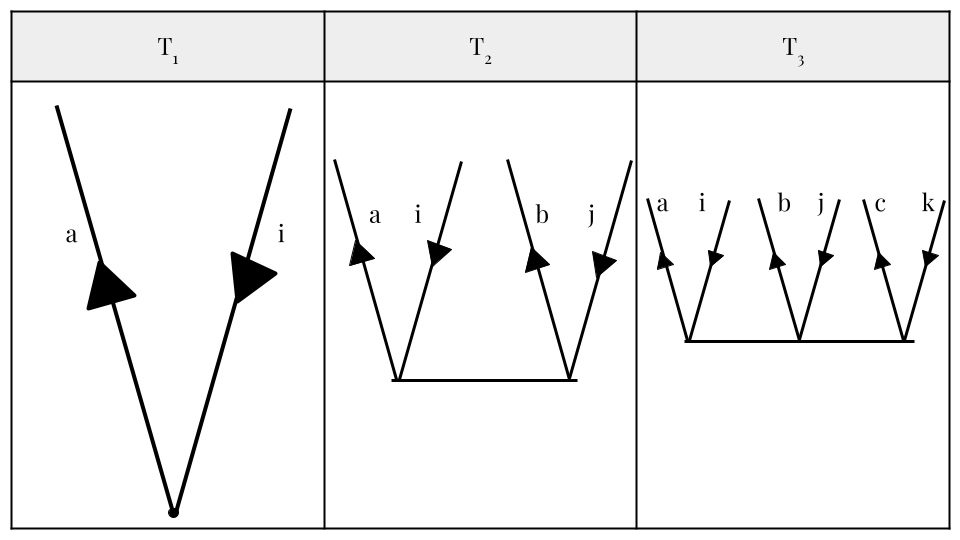
\includegraphics[scale=0.25]{Images/Chapter3/CC_diagrams.png}
    \caption{Diagrammatic representations for the $\hat{T}_1$, $\hat{T}_2$, and $\hat{T}_3$ operators.  Higher order $\hat{T}_m$ operators can be created using the pattern in the operators shown here.}
    \label{fig:T_diagrams}
\end{figure}

To show a complete coupled cluster calculation written out in diagrammatic form, we will represent the CCD amplitude equation in diagrammatic form in Eq. \ref{fig:ccd_amp}.  Though long, this collection of diagrams is significantly shorter than the entirely written out CCD amplitude equation using summations and Dirac notation, which can be found in Ref. \cite{Ref8}.

\begin{figure}
    \centering
    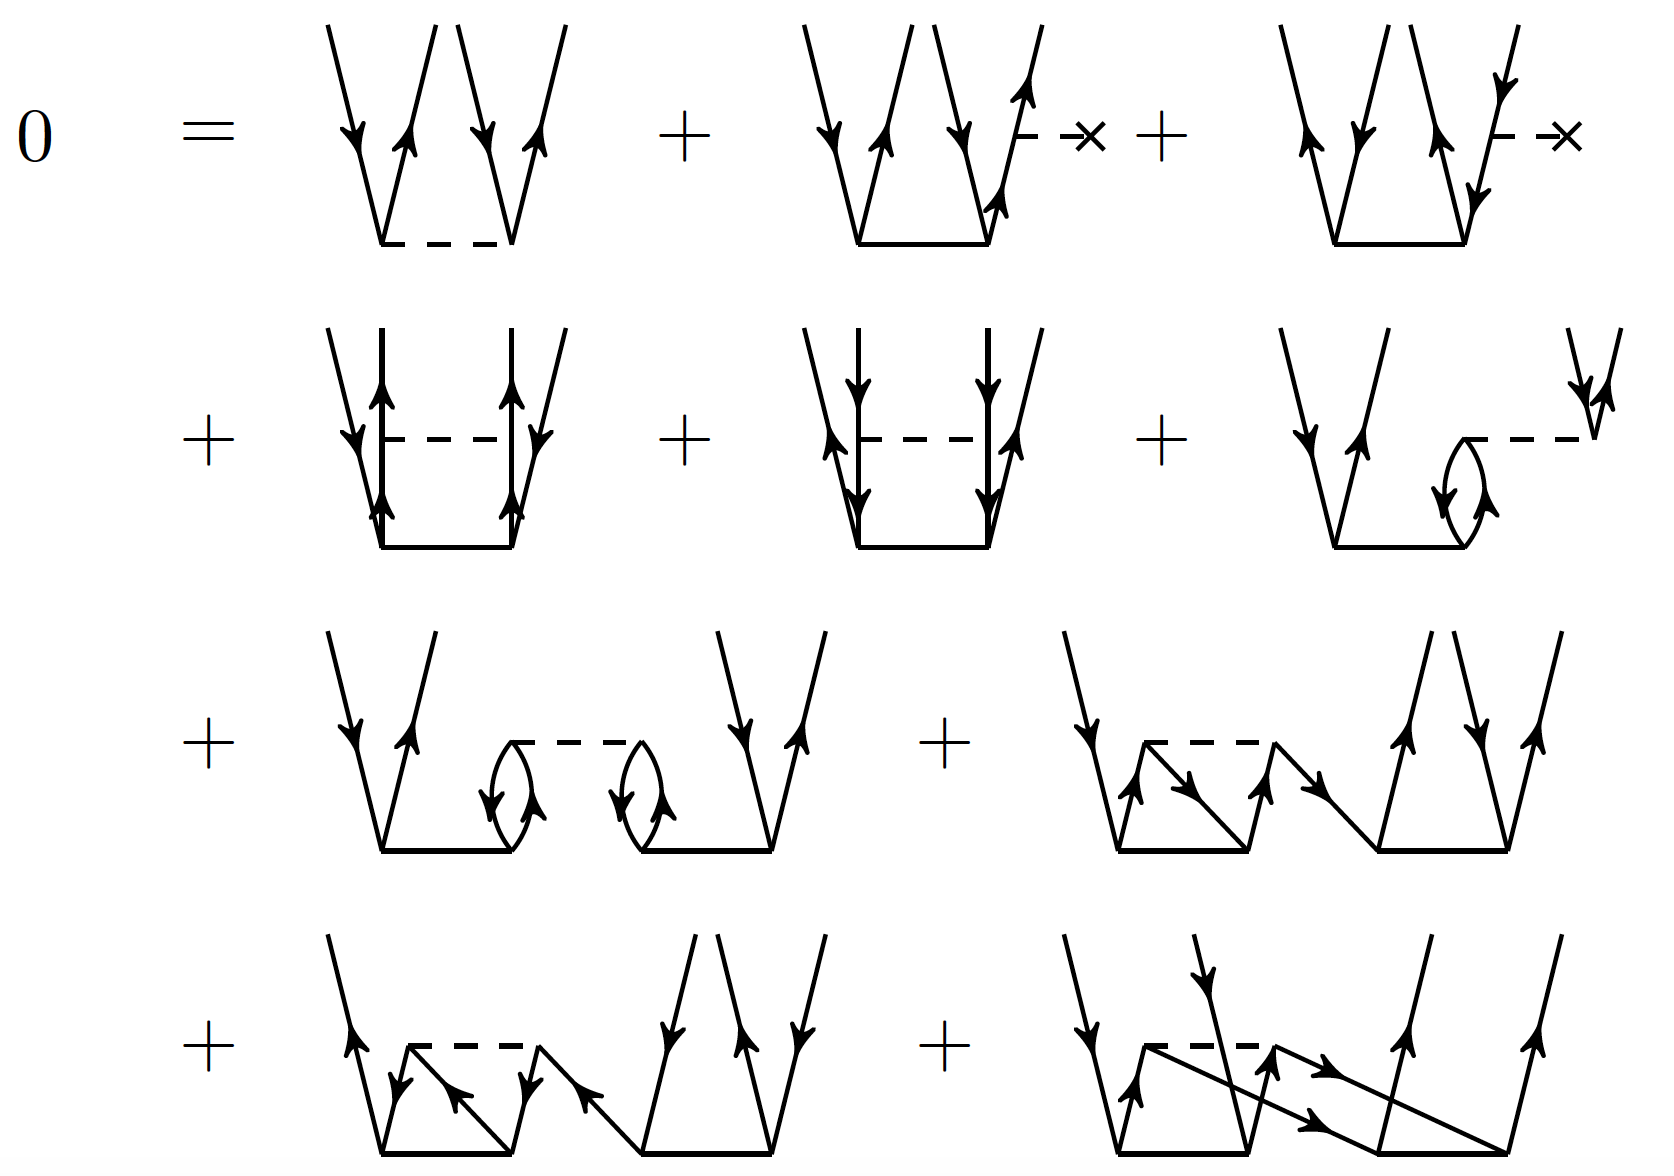
\includegraphics[scale=0.25]{Images/Chapter3/Diagrams-CCD.png}
    \caption{The diagrammatic formulation for the CCD amplitude equation.}
    \label{fig:ccd_amp}
\end{figure}



\begin{figure}
    \centering
    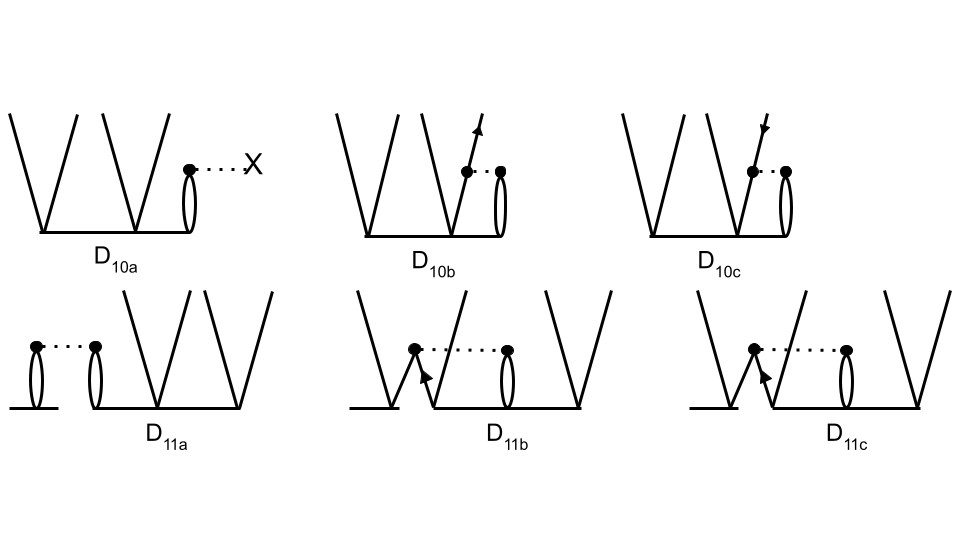
\includegraphics[scale=0.25]{Images/Chapter3/T3 to CCSDT T2.png}
    \caption{Antisymmetrized Goldstone diagrams representing the $\hat{T}_3$ contributions to the CCSDT $\hat{T}_2$ equations. D$_{10b}$ and D$_{10c}$ are relevant to the CCDT-1 approximation defined in the last section.}
    \label{fig:my_label}
\end{figure}

\begin{figure}
    \centering
    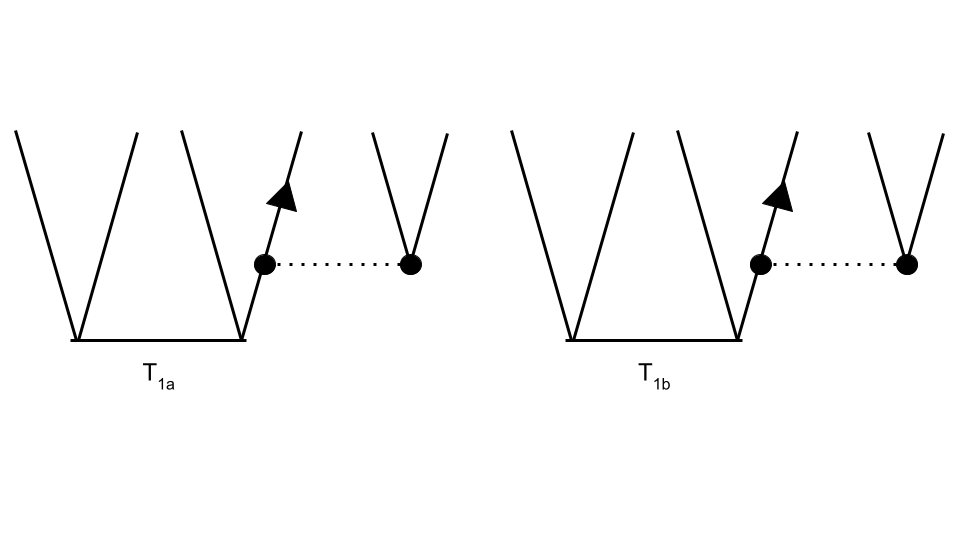
\includegraphics[scale=0.25]{Images/Chapter3/Relevant T3.png}
    \caption{Antisymmetrized Goldstone diagrams representing the CCSDT $\hat{T}_3$ equations relevant to calculating the CCDT-1 approximation. For a full list of all antisymmetrized Goldstone diagrams for the CCSDT $\hat{T}_3$ equations, the reader is referred to Ref. \cite{Ref21}.}
    \label{fig:my_label}
\end{figure}

Finally, look at some diagrams from the $\hat{T}_3$ operator, which are important to the CCD(T) and CCDT-1 approximations. In fact, the terms $T_{1a}$ and $T_{1b}$ from the $\hat{T}_3$ amplitude equations form  Eq. \ref{ccdt1_eq}.  The amplitudes that are gained by this equation are then used to calculate the diagrams $D_{10b}$ and $D_{10c}$ for the $\hat{T}_2$ amplitudes \cite{Ref156}.    

    \section{Many-Body Methods Conclusion}
        %%% THESIS CONCLUSIONS %%%

% SRE as a valid extrapolation method
The sequential regression extrapolation (SRE) method developed here based on Bayesian regression algorithms is an accurate and valuable extrapolator for removing basis incompleteness errors from coupled cluster calculations of infinite matter systems. Furthermore, when the infinite matter system needs to be taken to the thermodynamic limit, it is possible to use SRE to perform this task. Since the SRE algorithm uses training data taken from calculations at small numbers of single-particle states to predict the correlation energy at many single-particle states, the SRE algorithm can offer significant time savings over performing fully converged correlation energy calculations. As shown in this thesis, using the SRE algorithm to save over 100 node hours in the calculations of just one correlation energy is possible. Furthermore, this huge time savings does come with a loss in the accuracy of performing the whole savings. However, the average percent error between the SRE prediction and the fully calculated result was typically less than 1$\%$, making it quite a slight difference compared to the large amount of computational time that has been saved.

% From the CCD vs. CCDT side
Furthermore, besides developing the SRE method, we also compared different methods of performing coupled cluster calculations of systems of infinite nuclear matter. First, we compared the results from two different interactions: the Minnesota potential, a toy interaction, and chiral NNLO potentials, which are much more realistic. By comparing these two, we learned that they differ quite significantly around densities of infinite nuclear matter that are similar to nuclear densities and that calculations containing NNLO potentials do take much longer to compute compared to a Minnesota potential applied to the same system. Furthermore, we could also compare the difference between the coupled cluster approximations CCD, CCDT-1, and CCD(T) on calculations of infinite matter systems. We found that the triples approximations give significant results when compared to the CCD approximation, so they are worth performing even though they provide an increase in computational time.

%% SIZE OF MACHINE LEARNING SYSTEM
Though it has been mentioned throughout this thesis, it is essential to emphasize the size of the training data sets used in this work. This work's most extensive training data set used only 16 training points, and the smallest training set used only 3 points. Some areas of physics could be faster to adopt machine learning because of the vast amount of training data that some machine learning algorithms require. However, this work has shown that accurate machine learning predictions can be made with very few training points, thus encouraging using machine learning as a tool in fields with small data sets.

%%% FUTURE WORKS %%%

\subsection*{Possible Future Works}
% Full triples and different proton fractions
A few notable future works stem directly from the work presented here. First, while we showed results from both the CCD< CCDT-1, and CCD(T) approximations, we did not have the capabilities to produce coupled cluster correlation energies using a complete CCDT calculation. This is mainly due to the high computational costs of a complete triple calculation ($O(M^8)$), but advancements, such as those made in Refs. Furthermore, ADD REFERENCES HERE are making this a much more achievable goal for the near future.

Additionally, while we only looked at pure neutron matter and symmetric nuclear matter here, there are other proton fractions of interest. If we want to model the equation of the state of nuclear matter thoroughly, then we need to be able to accurately predict the properties of neutron matter at proton fractions beyond just 0.0 and 0.5.

% PARAGRAPH ABOUT NOT BEING LIMITED TO INFINITE SYSTEMS
While truncating the number of particles in a calculation is limited to infinite matter and other large systems, truncations occur in every \textit{ab initio} many-body calculation. Basis truncation is especially common and occurs in almost every calculation except some simple toy models. The last part of this thesis will be dedicated to exploring some possible future applications of the SRE methodology which has been developed.

% PARAGRAPH ABOUT CC CALCULATIONS OF THE NUCLEUS
An extension of the work presented in this thesis is to apply the SRE method to remove basis incompleteness errors from coupled cluster calculations of nuclei. Though nuclei are finite systems and the number of nucleons in the system generally does not need to be truncated, the number of single-particle states is still truncated, leading to a need to extrapolate to an infinite model space \cite{Ref6}. This is especially true for heavy nuclei and nuclei that are weakly bound \cite{Ref6}. There are methods to perform these extrapolations on nuclei calculations, but when using the harmonic oscillator basis, which mixes the ultraviolet and infrared cutoffs, these extrapolation methods can fail \cite{Ref6}. Machine learning has been used to perform similar extrapolations (see Ref. \cite{Ref6}, \cite{Ref22}, \cite{Ref23}, for example), but these were performed with neural networks and thus incurred all of the problems that were experienced with neural networks in this thesis.

%% MBPT CALCULATIONS AND HIGHER ORDERS
Additionally, the SRE method has no reason to be restricted to only predicting CC energies using MBPT2 energies. Extending the SRE method to other many-body methods should also be possible. 

% PARAGRAPH ABOUT FCI
One of the most accurate yet restricted \textit{ab initio} many-body methods is full configuration interaction theory (FCI), which uses a variationally optimized linear combination of the full set of Slater determinants. FCI is used in nuclear physics and electronic-structure theory, but its complexity limits it to only the smallest of systems. The ground state energy, which FCI finds, is the lowest (variationally) and most accurate that can be achieved. If an infinite single particle basis is used, FCI produces the solutions to the Schr\"{o}dinger equation. However, due to computational limitations, FCI calculations must be performed with a finite basis, meaning they will fail to retrieve the total energy \cite{Ref1}. However, it is possible that SRE could be applied to FCI calculations using, for example, Hartree Fock calculations as the "fast method" to quickly and accurately extrapolate FCI results to the infinite basis limit, thus recovering the Schr\"{o}dinger equation results.

 % APPLICATIONS OUTSIDE OF NUCLEAR PHYSICS
While most of this thesis, except for the sections on the electron gas, have been devoted to nuclear physics applications, \textit{ab initio} many-body methods occur in many other fields besides nuclear physics. For example, coupled cluster theory, and other many-body methods, are prevalent in other fields of physics and quantum chemistry. Therefore, the development of the SRE method should improve calculations outside of the realm in which it was developed.


%%%%%%%%%%%%%%%%%%%%%%%%%%%%%%
%% CHAPTER: INFINITE MATTER SYSTEMS
%%%%%%%%%%%%%%%%%%%%%%%%%%%%%%
\chapter{Infinite Matter Systems}
    %%%%%%%%%%%%%%%%%%%%%%%%%%%%%%
    %% Introduction to Infinite Matter Systems
    %%%%%%%%%%%%%%%%%%%%%%%%%%%%%%
    \section{Introduction to Infinite Matter Systems}
        \chapter*{Introduction}

%VMC methods pose a very attractive alternative to other more complex ways of finding the ground state energies of simple atoms and molecules, like configuration-interaction calculations. The price to be paid in exchange for this simplicity is the sensitivity to the trial wave functions that are used, a VMC algorithm is very sensitive to how these are constructed, so they are one of the most important aspects to be considered (in this work, given the simple nature of the atoms which we will be working with, it's not so important to worry about the quality of the trial wave functions because very simple and basic ones are more than enough to reproduce the actual results). It shouldn't be forgotten that it is a variational method, and this implies that finding the optimal set of variational parameters is going to be the most important part of the calculation itself because it would create a lot of problems if the search range for the parameters was illy defined and not close enough to the variational minimum, namely, the results would have a poor quality in this case. This means that the parameters need to be chosen very carefully, or a recursive search with decreasingly coarse spacing in the space of variational parameters is required if there is no deep knowledge about the system in question.

%Instead of evaluating a very complex multidimensional integral to compute the expectation value of an operator, like the hamiltonian in this case, a VMC calculation exploits the fact that the majority of the configuration space where the wave function belongs can be regarded as much less important than other parts, the values of the wave function are too small there and can be mostly ignored during the integration of the algorithm. To capitalize this, the Metropolis algorithm is added to the VMC method, as well as importance sampling and Gaussian Type Orbitals.

%\todo{motivasjon (QD i 2D og 3D + atomer -> fleksibel kode)}
%\subsubsection{Introducing the problem and the flexible solver}
Quantum mechanical systems are complex. As such creating a specific
program for each specific system is not a viable method of studying a
range of systems. We need to generalize. A generalized solver for
quantum mechanical systems must be written without any constraints to
specific properties any system may have. To achieve such a feat the
program is best implemented by the use of object orientation, creating
an easily expandable solver to which simple or complex systems may be
added. In this thesis the aim is to write a generalized variational
Monte Carlo solver which, by using object orientation, may handle a
wide range of quantum mechanical systems, such as confined electrons
in so-called quantum dots, atoms, and molecules.

%\subsubsection{Further introduction to the solver, the trial function, the slater determinant}
The variational Monte Carlo method poses an attractive way to solve
quantum mechanichal systems, compared to other more complex methods,
while also taking correlation factors into account, as opposed to the
Hartree-Fock method. The attractiveness of the variational Monte Carlo
method lies in the way it solves the multi-dimensional integrals
arising in the many-body quantum mechanical problem, which, as the
name implies, is by using the Monte Carlo method. In this thesis a
single so-called Slater determinant is used as an ansatz for the trial
wave function. This simplicity makes it easy to implement an efficient
and flexible program. It is however a compromise, yielding less
accurate results, but nevertheless good enough to study a variety of
systems.

%\subsubsection{Introducing the QD problem in 2 and 3 dimensions, and atoms. Tie to use of flexible code}
The solver presented in this thesis was initially made to solve simple
atomic systems, as a reference, and thereby expanding to molecules. To further
demonstrate the flexibility of the program, quantum dots are studied
in two and three dimensions. The reason for choosing quantum dots to
be studied is their simple structure, yet multitude of practical uses.


%\todo{hva jeg har gjort}
%\subsubsection{Introduce implementation of the code}


%\subsubsection{Short description of various tests done with QD and atoms}
The aim in this thesis is to demonstrate the flexibility of the
program by studying the system like atomic helium, beryllium and neon,
the helium and beryllium molecules, benchmarking ground state energies
against existing references, and studying their one-body densities. Furthermore
quantum dots consisting of up to 56 electrons will be studied in a
similar manner, and their frequency will be varied.  With a lower
frequency the quantum dots will implicity have a higher correlation,
and studying correlations are of great importance when using more
elaborate methods than for example the simple Hartree-Fock method.

Ground states of atoms and molecules are compared to experimental
results, which should be close to the exact results, offering a good
test of the accuracy of the variational Monte Carlo method and the
solver created. Because of the popularity of quantum dots several
master students have studied them, each with different methods. This
provides a wide range of references to which ground state energies may
be compared, which should give further insight to the accuracy of the
solver.

%\todo{oppgavens struktur}
%\subsubsection{Chapter by chapter}
The thesis is structured in two parts: a theory part, and a results part. A brief description of the chapters is given below.
\begin{itemize}
	\item In the first chapter a brief introduction to scientific computing is given. In it different types of programming languages will be described, and we will give an introduction to object-oriented programming. This is important because object-oriented programming is used to create a generalized solver. A summary of message passing interface, used to parallelize the computations, is also given.  
	\item The second chapter aims to give an overview of a more basic solution method, the Hartree-Fock method. It also describes other methods derived from the Hartree-Fock method, so-called post Hartree-Fock methods. The Hartree-Fock method can be used as a convenient test for a more simplified variational Monte Carlo program, and some of the post Hartree-Fock methods are used in computations of references when ground state energies computed by the solver is benchmarked.
	\item Next the variational Monte Carlo method is explained with details around ways of optimization, like the Metropolis algorithm and importance sampling. Details about how to calculate the Slater determinant efficiently and other measures to further optimize the solver are also given. Then the process of blocking to get an accurate estimate of the error is explained.
	\item In the fourth chapter the modelled systems are described. How quantum dots are modelled in two and three dimensions is described, then a brief descrition of how each of the atomic systems are modelled is given. A way to replace the Slater type orbitals with gaussian type orbitals is also described.
	\item In the final chapter of the first part we look at how the solver is structured, and how the variational Monte Carlo method is implemented using object-orientation.
	\item With the theory in place we look at the results from calculations with the variational Monte Carlo solver created. The program is benchmarked to test the optimizations and also to see how well it scales with an increasing number of processors used. The systems are benchmarked against reference ground state energies, and one-body densities are calculated, which can give insight into the structure of the systems. 
	\item Finally a conclusion is given with final remarks.
\end{itemize}


%`God does not play dice' Einstein said \todo{ref}, refuting the theory that quantum mechanical systems are governed by probability. However, as it turns out, we may, to solve them.


    %%%%%%%%%%%%%%%%%%%%%%%%%%%%%%
    %% Single Particle Basis for Infinite Matter
    %%%%%%%%%%%%%%%%%%%%%%%%%%%%%%
    \section{Single Particle Basis for Infinite Matter}
        We can begin to define a single particle basis for infinite matter calculations in three dimensions by defining the single particle wavefunction as plane waves with the form:

\begin{equation} \label{im_wavefunction}
	\psi_{\vec{k},\sigma} = \frac{1}{\sqrt{\Omega}} e^{i\vec{k}\cdot\vec{r}}\xi_\sigma,
\end{equation}

where $\xi_\sigma$ has two possible values corresponding to spin-up particles:

\begin{equation} \label{spin_up}
	\xi_{\sigma=\frac{1}{2}} = \begin{bmatrix}
									1 \\
									0 \\
								\end{bmatrix},
\end{equation}

or spin-down particles: 

\begin{equation} \label{spin_down}
	\xi_{\sigma=-\frac{1}{2}} = \begin{bmatrix}
									0 \\
									1 \\
								\end{bmatrix}.
\end{equation}


Additionally, in Eq. \ref{im_wavefunction}, $\Omega = L^3$ corresponds to the volume of the infinite matter system. The limit $L \rightarrow \infty$ is taken to accurately simulate an infinite matter system after the various expectation values have been calculated \cite{Ref3, Ref13, Ref1}.

When using the plane waves as the single particle wavefunctions and assuming periodic boundary conditions, we can define the single particle momentums to be:

\begin{equation} \label{sp_momentum}
	k_i = \frac{2\pi}{L}n_i,
\end{equation}

where $i$ = $x$, $y$, or $z$ and n$_i$ = 0, $\pm$1, $\pm$2, ... \cite{Ref3, Ref1}.  From the momentum numbers, we can define the kinetic energy of an infinite matter system in second quantization to be:

\begin{equation} \label{im_kinetic}
	\hat{T} = \sum_{\vec{p}\sigma_p} \frac{\hbar^2k_p^2}{2m}a^\dagger_{\vec{p}\sigma_p}a_{\vec{p}\sigma_p}.
\end{equation}

Finally, we can define the energy of each single particle state in terms of its quantum numbers:

\begin{equation} \label{sp_energy_n}
	\epsilon_{n_x,n_y,n_z} = \frac{\hbar^2}{2m}(\frac{2\pi}{L})^2(n_x^2 + n_y^2 + n_z^2).
\end{equation}

We can rewrite Eq. \ref{sp_energy_n} to be in terms of the momentum using Eq. \ref{sp_momentum}, resulting in:

\begin{equation} \label{sp_energy_k}
	\epsilon_{n_x, n_y, n_z} = \frac{\hbar^2}{2m}(k_x^2 + k_y^2 + k_z^2).
\end{equation}

%% ADD A SECTION HERE ABOUT THE FERMI LEVEL AND THE FERMI MOMENTUM

Some of the single-particle states in a system will contain particles, which we will call occupied single-particle states. On the other hand, some will not contain particles, referred to as unoccupied single-particle states. When the system is arranged in its ground state formation (i.e., the lowest energy configuration), the occupied single-particle states fill the states with the lowest single-particle energies. Thus, the occupied single particle states will lie inside a so-called Fermi sphere, described by the Fermi momentum, k$_F$, and the Fermi energy, E$_F$. The Fermi level divides the occupied and unoccupied single-particle states in this ground state configuration.

The following set of equations can relate to the Fermi momentum and the Fermi energy:


\begin{equation} \label{fermi_energy}
	E_f = \frac{\hbar^2k_f^2}{2m} \longrightarrow k_f = \sqrt{\frac{2mE_f}{\hbar^2}}.
\end{equation}

 From the Fermi momentum, we can define the average density of the system, $\rho_0$, to be:

\begin{equation} \label{density_fermi_momentum}
	\rho_0 = \frac{k_f^3}{3\pi^2}.
\end{equation}

The average density, $\rho_0$ can also be defined as $\rho_0 = N/\Omega$, where N is the number of particles in the system and like L, the limit $N \rightarrow \infty$ is taken. However, the limits $N, L \rightarrow \infty$ are taken such that $\rho_0$ remains at a fixed, finite value. Finally, N and k$_F$ can be related with:

\begin{equation}
	N = \frac{k_f^3\Omega}{3\pi^2} \longrightarrow k_F = (\frac{3\pi^2N}{\Omega})^{1/3}.
\end{equation}

While in this theoretical model, there are an infinite number of single-particle states in the basis, in practice, due to computational limitations, the total number of single-particle states included in the calculation, M, must be truncated to a finite number. In this work, we will assume that the number of occupied and unoccupied single particle states correspond to closed-shell structure, and the total number of shells will be finite. We will place a spherical energy cut-off on the quantum numbers such that n$_x^2$ + n$_y^2$ + n$_z^2$ $\leq$ N$_{shells}$-1, where N$_{shells}$ is the total number of energy shells included in the calculation. It is important to note that N$_{shells}$ $\neq$ N$_{max}$.  Rather N$_{max}$ corresponds to the maximum value of n$_{x}$, n$_{y}$, or n$_{z}$ that is included in the calculation. This closed shell structure is also used for coupled cluster calculations in Ref. \cite{Ref3}, \cite{Ref5}, and \cite{Ref8} among others.

Enforcing a closed-shell structure for the occupied and unoccupied single-particle states and truncating the total number of shells allowed in the system restricts the number of allowed particles and total single-particle states to a finite set of values. We refer to these allowed numbers as "magic numbers," They correspond to the total number of single-particle states when s shells are included in a calculation. The first magic number is two, as there are two single-particle states in the first energy shell. The second magic number is 14, as there are 14 single-particle states when two energy shells are included (2 in the first shell and 12 in the second shell). Continuing as such gives the following magic numbers: 2, 14, 38, 54, 66, 114, ... .  Note that these are only the magic numbers for the homogeneous electron gas and pure neutron matter. For symmetric nuclear matter, all magic numbers are doubled (4, 28, 76, 108, 132, 228, ...). In the context of this thesis, the term shells will refer to the total number of energy shells used in the calculation, $M$ will refer to the total number of single-particle states in the system (both occupied and unoccupied), and open shells will refer to the number of shells above the Fermi level only.

    %%%%%%%%%%%%%%%%%%%%%%%%%%%%%%
    %% The Homogeneous Electron Gas
    %%%%%%%%%%%%%%%%%%%%%%%%%%%%%%
    \section{The Homogeneous Electron Gas}
        The homogeneous electron gas (HEG) is an infinite matter system containing only electrons with a uniform positive background charge such that the overall net charge of the system is zero \cite{Ref4}. Though the HEG as a theoretical model exists in one, two, and three dimensions \cite{Ref4}, this thesis will only focus on the three-dimensional electron gas. The HEG in three dimensions is essential in density functional theory, where it is the cornerstone of the local density approximation \cite{Ref4}. It is also a reasonable model for several systems of interest in quantum chemistry and condensed matter physics, including the electrons in semiconductors and alkali metals \cite{Ref4}. Additionally, studies of the HEG can be used to build a framework that can be transferred to studies of infinite nuclear matter, which is essential for studying the equation of the state of nuclear matter and many-body studies of neutron stars. The HEG is used as a framework for developing analysis tools for other many-body systems because the HEG is a relatively simple infinite matter system, leading to many published properties (both analytical and numerical) for results to be compared to. Other studies have used the HEG as a system that allows for comparisons between the results of different many-body methods (see, for example, Ref. \cite{Ref4}).

The Hamiltonian for the HEG consisting of $N$ electrons can be defined as

\begin{equation}
    \hat{H} = \hat{K} + \hat{V}_{ee} + \hat{V}_{be} + \hat{V}_{bb},
\end{equation}

where $\hat{K}$ is the kinetic energy operator, $\hat{V}_{ee}$ is the interaction between all sets of two electrons, $\hat{V}_{be}$ describes the interaction of all electrons with the positive background charge, and $\hat{V}_{bb}$ describes the contribution of the background charge interacting with itself. Since the HEG comprises a positively charged background and negatively charged electrons, the Coulomb force is the primary force at play in the interactions. The Coulomb force is a long-range force that acts over an infinite space. However, instead of using the Coulomb interaction, we will instead use Ewald's interaction, which splits the electron interaction into a short-range term and a long-range term while simultaneously dealing with $\hat{V}_{be}$ and $\hat{V}_{bb}$. We can rewrite the HEG Hamiltonian using the Ewald interaction as:

\begin{equation}
    \hat{H} = -\frac{1}{2}\sum_\alpha \nabla^2_\alpha + \frac{1}{2}\sum_{\alpha \neq \beta}\hat{v}_{\alpha\beta} + \frac{1}{2}Nv_M,
\end{equation}

where $\alpha$ and $\beta$ are electron indices \cite{Ref1}.  The first term is the kinetic energy operator, and the final two terms comprise the Ewald interaction \cite{Ref1}. The term $v_M$ is called the Madelung term and $\hat{v}_{\alpha\beta}$, the two-electron operator, is defined as:

\begin{equation}\label{two_electron_operator}
    \hat{v}_{\alpha\beta} = \frac{1}{V}\sum_{\vec{q}} v_{\vec{q}}\ e^{i\vec{q}(\vec{r}_\alpha - \vec{r}_\beta)},
\end{equation}

where $V = L^3$ is the finite volume of the HEG and $v_{\vec{q}} = \frac{4\pi}{{\vec{q}}^2}$ if $\vec{q} \neq 0$ and $v_{\vec{q}} = 0$ if $\vec{q} = 0$ \cite{Ref1}. This choice of Hamiltonian leads to the plane wave basis for the single-particle states described in Section 2 of this chapter. While the Ewald interaction makes the HEG easier to work with by splitting up the long-range and short-range components of the electron-electron interaction, it cannot correctly describe the exchange-correlation energy \cite{Ref4}.

Note that the density of the homogeneous electron gas is typically described by a parameter called the Wigner-Seitz radius. The Wigner-Seitz radius can be defined as

\begin{equation}
    r_s = \frac{r_0}{r_B},
\end{equation}

where r$_B$ is the Bohr radius, and r$_0$ is related to the size of the box containing the electron gas by

\begin{equation}
    \frac{4}{3}\pi r_0^3 = \frac{N}{L^3},
\end{equation}

where the density of the HEG is $d = N/L^3$, measured in fm$^{-3}$ \cite{Ref5}. A larger value of r$_s$ means the modeled system is in a larger box and therefore is less dense than a smaller value of r$_s$ for the same number of particles. It is important to note that the HEG behaves differently at different densities. At low densities (or high r$_s$), the electrons in the HEG are for a lattice. This process is called Wigner crystallization and results from the long-range repulsive interactions between the electrons \cite{Ref4}. At higher densities (or lower values of r$_s$), the HEG can better be described as a liquid instead of as a gas \cite{Ref4}.


The convergence of the correlation energy for the electron gas using plane waves as a basis has yet to be thoroughly investigated, but some work has been done in Ref. \cite{Ref1}. One reason why the correlation energy of the electron gas is an interesting problem is that it has substantial contributions from the electron-electron cusp. However, this electron-electron cusp does lead to trouble when making computational truncations as a finite set of single-particle states cannot accurately describe the behavior in this region \cite{Ref1}.

It is important to note that the MBPT2 correlation energies are well-defined for a finite electron gas. However, they diverge in the thermodynamic limit of an infinite electron gas in three dimensions \cite{Ref1}. This happens at high densities due to the dominance of the particle-hole ring diagrams \cite{Ref4}.

The single particle energies of the HEG when using the Ewald interaction are as follows for occupied single particle states:

\begin{equation}
    \epsilon_i = \frac{\vec{k}_i^2}{2} - \sum_{j\neq i} \langle ij| \hat{v}_2 | ji \rangle - \frac{v_M}{2},
\end{equation}

and for unoccupied single particle states:

\begin{equation}
    \epsilon_a = \frac{\vec{k}_a^2}{2} - \sum_j \langle aj | \hat{v}_2 | ja \rangle.
\end{equation}

Here we have used the common denotation of indices where $a$, $b$, $c$,... represent states which are unoccupied in the Fermi ground state, $i$, $j$, $k$,... represent states which are occupied in the Fermi ground state, and $p$, $q$, $r$,... could represent either \cite{Ref1}. 

We can also define the two-electron matrix elements in integral notation as:

\begin{equation}
    \langle ij | \hat{v}_2 | ab \rangle = \delta_{ia}\delta_{jb} \frac{1}{\Omega^2}\int \int d\vec{r}_1 d\vec{r}_2 \psi^*_i(\vec{r}_1)\psi^*_j(\vec{r}_2)\hat{v}_2(\vec{r}_1, \vec{r}_2)\psi_a(\vec{r}_1)\psi_b(\vec{r}_2),
\end{equation}

where $\hat{v}_2$ is defined in Eq. \ref{two_electron_operator} and $\psi$ are plane waves defined in Sec. 4.2.

By convention, the energies calculated using the HEG will be reported in Hartrees (1 Hartree = $4.35x10^{-18}$ Joules). However, this differs from the unit that will be used for the next system, infinite nuclear matter.


    %%%%%%%%%%%%%%%%%%%%%%%%%%%%%%
    %% Nuclear Forces
    %%%%%%%%%%%%%%%%%%%%%%%%%%%%%%
    \section{Interlude: Nuclear Forces}
        The properties of infinite nuclear matter and finite nuclear systems are determined by the nuclear forces that govern the interactions between the nucleons. These nuclear forces are given by two fundamental forces: the strong nuclear force, which binds the nucleons together, and the electromagnetic force, which causes repulsion between the protons. The strong force is stronger over short distances (which causes nuclei to hold together), but the electromagnetic force is a long-range force acting over large distances. The nature of the strong force needs to be better understood, and this can make it challenging to model the nuclear forces in theoretical calculations \cite{Ref200, Ref201}. Because of this, the interaction used to model the nuclear forces in this notebook is the "toy" interaction called the Minnesota potential, which is defined in Ref. \cite{Ref166} and used in, for example, Refs \cite{Ref3, Ref5, Ref167} to model the nuclear interaction. The Minnesota potential is a local, nucleon-nucleon-only, moderately soft potential reproducing the nucleon-nucleon effective range parameters. It provides a reasonable approximation for the binding energies of light nuclei, but it is a simple interaction that is computationally inexpensive compared to more realistic nuclear interactions. It should be noted that the Minnesota potential is a phenomenological interaction, meaning that it was constructed by fitting experimental data instead of being derived from first principles. The matrix elements for the Minnesota potential are given by:

$$V_{i,j} = \frac{1}{2}[V_R + \frac{1}{2}(1+P^\sigma_{ij})V_t + \frac{1}{2}(1-P^\sigma_{ij})V_s](1+P^r_{ij}).$$

In the above equation, $P^\sigma$ is the spin exchange operator, $P^r$ is the space exchange operator, and V$_R$, V$_t$, and V$_s$ are given by the following equations, where r$_{ij}$ is the distance between two nucleons and the constants are found by fitting to experimental data.

$$V_R = V_{0R}e^{-\kappa_Rr_{ij}^2}$$

$$V_t = -V_{0t}e^{-\kappa_tr_{ij}^2}$$

$$V_t = V_{0s}e^{-\kappa_sr_{ij}^2}.$$

Though the Minnesota potential is computationally inexpensive and captures important aspects of the nuclear interactions, modern advancements have improved our models of nuclear forces \cite{Ref20, Ref122, Ref43, Ref200, Ref201, Ref202, Ref203, Ref204, Ref123, Ref125,Ref129, Ref130, Ref131, Ref132, Ref133, Ref134, Ref138}. The second nuclear force used to model infinite nuclear matter in this thesis, which is a more model interaction, is derived from practical field theory (EFT) \cite{Ref3} \cite{Ref38, Ref16, Ref42, Ref43, Ref44, Ref45, Ref46, Ref47, Ref48, Ref49, Ref50, Ref200, Ref201}. The nuclear forces derived from EFT have an advantage over other nuclear forces in that the two-body and the many-body interactions can be derived in a mutually consistent matter \cite{Ref8}. Much recent progress has been made in deriving the nuclear forces based on chiral EFT and the nuclear Hamiltonian for many nucleonic matter calculations, not using forces from chiral EFT, including both nucleon-nucleon (NN) and three-nucleon (3N) forces \cite{Ref123, Ref129, Ref138, Ref139, Ref146, Ref122, Ref131}. For the results presented herein, we will use the parametrization NNLO$_{opt}$ for the NN and local 3N interactions.  

It should be noted that implementing the 3N forces in the single particle basis used for infinite nuclear matter calculations is much simpler than implementing them in the harmonic oscillator basis commonly used for nuclei calculations \cite{Ref9}. However, the large number of matrix elements needed to compute 3N forces is still the computationally limiting factor in these calculations \cite{Ref9}.

The specific chiral potentials used in this work are detailed in Refs. \cite{Ref200} and \cite{Ref201}.  They have optimized $\Delta$-full interactions and are calibrated with nuclear matter properties \cite{Ref200}. The $\Delta$-full interaction is detailed in Refs. \cite{Ref202, Ref203, Ref204, Ref205, Ref206, Ref207}.  The interaction employs a standard non-local regulator function of the form:

\begin{equation}
    f(p) = e^{(p/\Lambda)^{2n}},
\end{equation}

where $p$ is the relative momentum, $n$ is 4, and $\Lambda$ is 394 MeV. We are using these interactions at the next-to-next-to-leading order (NNLO). In this order, 17 low-energy coefficients (LECs) parameterize the interaction and whose values are given in Ref. \cite{Ref200}. This leads to a form of the Hamiltonian, which can be written as:

\begin{equation}
    H(\alpha) = h_0 + \sum_{i=1}^{N_{LECs}=17}\alpha_ih_i,
\end{equation}

where $h_0 = t_{kin} + v_0$,  $t_{kin}$ is the kinetic energy, $v_0$  is a constant potential that does not depend on the LECs, $\vec{\alpha}$ is a vector that denotes all of the LEC.  Of the two interactions used in this thesis to model nuclear forces, the optimized $\Delta$-full interaction is more accurate than the Minnesota potential, but has more complex matrix elements which leads to longer run times.

    %%%%%%%%%%%%%%%%%%%%%%%%%%%%%%
    %% Infinite Nuclear matter
    %%%%%%%%%%%%%%%%%%%%%%%%%%%%%%
    \section{Infinite Nuclear Matter}
        Infinite nuclear matter is defined as a system containing infinite nucleons (protons and neutrons) that only interact via the nuclear forces \cite{Ref8}. Studies of infinite nuclear matter are essential for understanding the matter within dense astronomical objects such as neutron stars \cite{Ref3}. Neutron stars are exciting because they offer insights into nuclear processes and astrophysical observables. However, neutrons stars also contain matter that spans several orders of magnitude and contain many different compositions of matter \cite{Ref3,Ref35,Ref36,Ref37,Ref38,Ref39,Ref41}. Neutron star matter occurs at densities of 0.1 fm$^{-3}$ or greater and consists of various fractions of neutrons, protons, electrons, and muons. These particles exist in beta equilibrium ($\beta$-equilibrium) governed by the weak force.

Studies of infinite nuclear matter are also focused on determining the equation of state (EoS) . When considering applications to neutron stars, the EoS can help determine the mass range, the relationship between the star's mass and its radius, the thickness of the star's crust, and the rate at which the star will cool down \cite{Ref3}. Determination of the EoS also links neutron stars to the neutron skin in atomic nuclei and the symmetry energy of nuclear matter . Symmetry energy is crucial because it relates to the difference between proton and neutron radii in nuclei \cite{Ref8}.

Solving the EoS depends on our ability to solve the many-body problem for infinite nuclear matter \cite{Ref3,Ref8}. The nuclear matter has been of interest in many-body studies since the early days of the field (see Ref. \cite{Ref51} for a review of these early studies). These early calculations were performed with Brueckner-Bethe-Goldstone theory (\cite{Ref52,Ref53}). However, modern many-body studies of nuclear matter are performed with a varied of methods, including coupled-cluster theory (CC) (\cite{Ref3,Ref4,Ref5,Ref8,Ref9,Ref16,Ref43,Ref47}), Monte Carlo methods (\cite{Ref33,Ref54,Ref55,Ref56,Ref57,Ref58,Ref59,Ref60,Ref61}), Green's function methods (\cite{Ref50,Ref62,Ref63,Ref64}) and methods from the renormalization group theory family (\cite{Ref48,Ref3,Ref65}). The coupled-cluster theory will be the many-body method of interest for the remainder of this thesis. Coupled-cluster calculations of nuclear matter date back to the 1970s and 1980s \cite{Ref8}.

One property of infinite nuclear matter we are interested in is the proton fraction, which is defined as 
\begin{equation}\label{proton_fraction}
    x_p = \frac{\rho_p}{\rho},
\end{equation}
where $\rho_p$ is the density of protons in the matter, $\rho_n$ is the denisty of neutrons in the matter, and $\rho$ = $\rho_p$ + $\rho_n$ is the total density of the infinite nuclear matter \cite{Ref3}.  Defining different proton fractions defines different types of infinite nuclear matter systems. For example, if $x_p$ = 0, the infinite nuclear matter system contains only neutrons. We will refer to this system as pure neutron matter (PNM). If $x_p$ = 1/2, then the system contains an equivalent number of protons and neutrons, and this system is called symmetric nuclear matter (SNM). 

From the proton fraction, we can define symmetry energy as the difference between the energy for pure neutron matter and symmetric nuclear matter at a set density. \cite{Ref3}

\begin{equation}
    E_{sym}(\rho) = E(\rho, x_p=0) - E(\rho, x_p=1/2) 
\end{equation}

All energies for infinite nuclear matter calculations will be, by convention, reported in units of MeV.


    %%%%%%%%%%%%%%%%%%%%%%%%%%%%%%
    %% Truncation Errors
    %%%%%%%%%%%%%%%%%%%%%%%%%%%%%%
    \section{Truncation Errors in Infinite Matter Calculations}
        As mentioned throughout this chapter, several truncations and approximations must be made to study these infinite matter systems in a computational framework. Though computational limitations require these truncations and approximations, they introduce errors into the calculations, making them undesirable \cite{Ref1, Ref2}. Though it is impossible to remove every error that comes from the various truncations and approximations, this thesis will focus on mitigating the effects of three truncation errors: the error that results from truncating the number of single-particle states in the basis, the error that results from truncating the number of particles and volume of the infinite matter system, and the error that results from truncating the coupled cluster correlation operator, $\hat{T}$.

% truncation of M basis incompleteness error
As discussed in Section 2 of this chapter, the number of single-particle states ($M$) in the calculation is truncated due to truncating the total number of energy shells allowed in the system. This introduces an error in the calculation called the basis incompleteness error. The basis incompleteness error can be mitigated by increasing the number of single-particle states (or energy shells) in the calculation. Unfortunately, this also drastically increases the computational time and resources needed. Coupled cluster theory has polynomial time scaling with respect to $M$, which, while being better than other many-body methods, still means that computational times can be prohibitive at large values of $M$.  Additionally since increasing the number of single-particle states in the system increases the number of matrix elements in the calculations, computational resources are also increased.

% truncation of N finite size effects
While infinite matter systems theoretically contain infinite particles over an infinite volume, these values must be truncated to finite values computationally \cite{Ref8}. This introduces an error in the calculations called finite size error. Since the number of particles in the system and the volume of the system are related by a fixed density ($\rho_0 = N/\Omega$), it is sufficient to increase $N$ to the infinite limit while keeping the density constant. However, the same problem occurs when attempting to increase $M$ since coupled cluster theory also has polynomial time scaling with respect to the number of particles in the system; however, the power tends to be higher with particles than with single-particle states. Additionally, matrix elements involving occupied states (or particles) are computationally more complex than those involving only unoccupied states. Therefore, adding more particles to the system increases the computational resources needed than additional single-particle states.

% reiterate the truncation of coupled cluster 
As discussed in the previous chapter, the coupled cluster correlation operator is:

\begin{equation} \label{T_repeat}
	\hat{T} = \sum_{m=1}^N \hat{T}_m,
\end{equation}

where $N$ is the total number of particles in the system and $\hat{T}_m$ represents the $m$-particle $m$-hole excitation operator. We can make this operator specific to infinite matter systems by making two changes. First, infinite matter systems contain particles, so $N = \infty$. Second, the 1-particle 1-hole excitation operator, $\hat{T}_1$, will always be zero for infinite matter systems due to symmetry. Therefore, we can write the cluster operator for infinite matter systems as:

\begin{equation} \label{T_repeat2}
	\hat{T} = \sum_{m=2}^\infty \hat{T}_m.
\end{equation}

Also, as discussed in the previous chapter, the correlation operator is truncated in practice by setting excitation operators over a certain level to zero. In this thesis, the coupled cluster results will either be calculated using coupled cluster doubles (CCD) where $\hat{T} \approx T_2$ or approximations to coupled cluster doubles triples (CCDT) where $\hat{T} \approx T_2 + T_3$. Since the full cluster operator is not used in the calculations, this does reduce the accuracy of the calculations. However, in this thesis, we will not be extrapolating to the complete coupled cluster calculation since this would require performing coupled cluster calculations at more truncation levels. However, we will attempt to improve the accuracy of infinite matter calculations by predicting the CCDT result from the CCD result and the CCD result from the MBPT2 result, thus improving the accuracy while keeping computational time and resources small.


However, in the infinite matter calculations, there are sources of error from approximations and truncations that are not addressed in this thesis but could be the subject of future work. Some of them will be discussed briefly here. First, the Coulomb interaction, the predominant interaction in the homogeneous electron gas, is a long-range interaction that acts over an infinite distance. Truncating the volume of the electron gas to a finite size also truncates the Coulomb interaction. It is important to note that this is a finite size error occurring in the HEG but not in infinite nuclear matter \cite{Ref4}. This means that studies of the HEG at finite sizes will face additional complications compared to studies of infinite nuclear matter \cite{Ref4}. In addition to truncating the coupled cluster correlation operator, not all n-body interactions are included in the calculation because the Hamiltonian is also truncated. In this work, calculations are limited to including, at most, the 2-body or 3-body matrix elements. However, the highest level of matrix elements contributing to the system is $N$-body, where $N$ is the total number of particles. Finally, while the Coulomb interaction, the primary interaction of the electron gas has a simple closed-form representation that can be calculated precisely, the primary interaction in the infinite nuclear matter is the nuclear interaction, dominated by the strong force. However, the nuclear interaction has no simple closed-form solution and cannot be represented precisely. Therefore all nuclear interactions are approximations with various levels of accuracy compared to real nuclear interaction.

%% PREVIOUS WORKS TO CORRECT THESE ERRORS WITH TRADITIONAL EXTRAPOLATION    

    \section{Conclusion}
        %%% THESIS CONCLUSIONS %%%

% SRE as a valid extrapolation method
The sequential regression extrapolation (SRE) method developed here based on Bayesian regression algorithms is an accurate and valuable extrapolator for removing basis incompleteness errors from coupled cluster calculations of infinite matter systems. Furthermore, when the infinite matter system needs to be taken to the thermodynamic limit, it is possible to use SRE to perform this task. Since the SRE algorithm uses training data taken from calculations at small numbers of single-particle states to predict the correlation energy at many single-particle states, the SRE algorithm can offer significant time savings over performing fully converged correlation energy calculations. As shown in this thesis, using the SRE algorithm to save over 100 node hours in the calculations of just one correlation energy is possible. Furthermore, this huge time savings does come with a loss in the accuracy of performing the whole savings. However, the average percent error between the SRE prediction and the fully calculated result was typically less than 1$\%$, making it quite a slight difference compared to the large amount of computational time that has been saved.

% From the CCD vs. CCDT side
Furthermore, besides developing the SRE method, we also compared different methods of performing coupled cluster calculations of systems of infinite nuclear matter. First, we compared the results from two different interactions: the Minnesota potential, a toy interaction, and chiral NNLO potentials, which are much more realistic. By comparing these two, we learned that they differ quite significantly around densities of infinite nuclear matter that are similar to nuclear densities and that calculations containing NNLO potentials do take much longer to compute compared to a Minnesota potential applied to the same system. Furthermore, we could also compare the difference between the coupled cluster approximations CCD, CCDT-1, and CCD(T) on calculations of infinite matter systems. We found that the triples approximations give significant results when compared to the CCD approximation, so they are worth performing even though they provide an increase in computational time.

%% SIZE OF MACHINE LEARNING SYSTEM
Though it has been mentioned throughout this thesis, it is essential to emphasize the size of the training data sets used in this work. This work's most extensive training data set used only 16 training points, and the smallest training set used only 3 points. Some areas of physics could be faster to adopt machine learning because of the vast amount of training data that some machine learning algorithms require. However, this work has shown that accurate machine learning predictions can be made with very few training points, thus encouraging using machine learning as a tool in fields with small data sets.

%%% FUTURE WORKS %%%

\subsection*{Possible Future Works}
% Full triples and different proton fractions
A few notable future works stem directly from the work presented here. First, while we showed results from both the CCD< CCDT-1, and CCD(T) approximations, we did not have the capabilities to produce coupled cluster correlation energies using a complete CCDT calculation. This is mainly due to the high computational costs of a complete triple calculation ($O(M^8)$), but advancements, such as those made in Refs. Furthermore, ADD REFERENCES HERE are making this a much more achievable goal for the near future.

Additionally, while we only looked at pure neutron matter and symmetric nuclear matter here, there are other proton fractions of interest. If we want to model the equation of the state of nuclear matter thoroughly, then we need to be able to accurately predict the properties of neutron matter at proton fractions beyond just 0.0 and 0.5.

% PARAGRAPH ABOUT NOT BEING LIMITED TO INFINITE SYSTEMS
While truncating the number of particles in a calculation is limited to infinite matter and other large systems, truncations occur in every \textit{ab initio} many-body calculation. Basis truncation is especially common and occurs in almost every calculation except some simple toy models. The last part of this thesis will be dedicated to exploring some possible future applications of the SRE methodology which has been developed.

% PARAGRAPH ABOUT CC CALCULATIONS OF THE NUCLEUS
An extension of the work presented in this thesis is to apply the SRE method to remove basis incompleteness errors from coupled cluster calculations of nuclei. Though nuclei are finite systems and the number of nucleons in the system generally does not need to be truncated, the number of single-particle states is still truncated, leading to a need to extrapolate to an infinite model space \cite{Ref6}. This is especially true for heavy nuclei and nuclei that are weakly bound \cite{Ref6}. There are methods to perform these extrapolations on nuclei calculations, but when using the harmonic oscillator basis, which mixes the ultraviolet and infrared cutoffs, these extrapolation methods can fail \cite{Ref6}. Machine learning has been used to perform similar extrapolations (see Ref. \cite{Ref6}, \cite{Ref22}, \cite{Ref23}, for example), but these were performed with neural networks and thus incurred all of the problems that were experienced with neural networks in this thesis.

%% MBPT CALCULATIONS AND HIGHER ORDERS
Additionally, the SRE method has no reason to be restricted to only predicting CC energies using MBPT2 energies. Extending the SRE method to other many-body methods should also be possible. 

% PARAGRAPH ABOUT FCI
One of the most accurate yet restricted \textit{ab initio} many-body methods is full configuration interaction theory (FCI), which uses a variationally optimized linear combination of the full set of Slater determinants. FCI is used in nuclear physics and electronic-structure theory, but its complexity limits it to only the smallest of systems. The ground state energy, which FCI finds, is the lowest (variationally) and most accurate that can be achieved. If an infinite single particle basis is used, FCI produces the solutions to the Schr\"{o}dinger equation. However, due to computational limitations, FCI calculations must be performed with a finite basis, meaning they will fail to retrieve the total energy \cite{Ref1}. However, it is possible that SRE could be applied to FCI calculations using, for example, Hartree Fock calculations as the "fast method" to quickly and accurately extrapolate FCI results to the infinite basis limit, thus recovering the Schr\"{o}dinger equation results.

 % APPLICATIONS OUTSIDE OF NUCLEAR PHYSICS
While most of this thesis, except for the sections on the electron gas, have been devoted to nuclear physics applications, \textit{ab initio} many-body methods occur in many other fields besides nuclear physics. For example, coupled cluster theory, and other many-body methods, are prevalent in other fields of physics and quantum chemistry. Therefore, the development of the SRE method should improve calculations outside of the realm in which it was developed.

%%%%%%%%%%%%%%%%%%%%%%%%%%%%%%
%% CHAPTER: BAYESIAN MACHINE LEARNING
%%%%%%%%%%%%%%%%%%%%%%%%%%%%%%
\chapter{Bayesian Machine Learning}
    %%%%%%%%%%%%%%%%%%%%%%%%%%%%%%
    %% Machine Learning
    %%%%%%%%%%%%%%%%%%%%%%%%%%%%%%
    \section{Machine Learning}
        % What is machine learning?
Machine learning is the field that occurs at the intersection of data science and artificial intelligence; it is the science of programming a computer so that it can learn from a given data set \cite{Ref12}. Machine learning algorithms can solve these problems without being programmed with task-specific instructions; machine learning encompasses a set of generic algorithms that can be applied to various problems.

% When is machine practical learning?
Machine learning can be applied to a wide variety of problems, but it is most useful when traditional styles of programming cannot solve the problem or would take a very long time to solve a problem. This includes problems where the traditional solution would have a long list of rules; machine learning can find patterns in the data set without problem-specific programming. Machine learning also excels in problems where a large amount of complex data is difficult to sort and work with by hand or with traditional programming \cite{Ref12}.


% Briefly explain some classifications of machine learning
Machine learning algorithms can be classified into one of three categories: supervised, unsupervised, and reinforcement learning. In supervised learning, the training data given to the algorithm is labeled, meaning it has both an X and a y component. Therefore, supervised learning aims to map every X to its corresponding y correctly. There are two types of supervised learning: classification (when y contains a finite number of possible values) and regression (when y contains an infinite number of possible values). All machine learning algorithms developed in this chapter will be supervised learning. Unsupervised learning algorithms work with unlabelled data, meaning they only receive the X component of the data set. Common unsupervised learning tasks are clustering and dimensionality reduction. Finally, reinforcement learning describes a set of algorithms where an agent learns to solve a problem by maximizing its reward. Supervised and unsupervised learning are common in machine learning applications in physics, while reinforcement learning in physics applications is less common.  

% INTRODUCTION
Machine learning has recently become a popular tool in physics and is being applied to a wide range of problems. Machine learning has found applications across all areas of physics. Specifically looking at neural networks, they have been used in nuclear physics to perform extrapolations (for example Refs. \cite{Ref24}, \cite{Ref25}, \cite{Ref26},\cite{Ref27},\cite{Ref28},\cite{Ref29},\cite{Ref30},\cite{Ref31}) and to directly solve the many-body problem (for example Ref \cite{Ref32}).  Neural networks can be problematic for \textit{ab initio} data sets due to very small data sets, but will be explored in this thesis as a possible machine learning method.  Machine learning can also be used in many-body physics to simulate the wavefunction of a system to find the variationally lowest energy of the system {ADD REFERENCES}.  More generally, machine learning algorithms have been used to predict the coupled cluster energies of molecules using a variety of machine learning algorithms.  The work presented in this thesis, though unique, has been inspired by these previous applications of machine learning in the field of many-body physics. 

% Explain the structure of the chapter
The remainder of this chapter will be structured as follows. The following sections will develop four standard supervised learning algorithms: linear regression, its related algorithms ridge and kernel ridge regression, and finally, a brief discussion on neural networks and recurrent neural networks. Next, there will be a discussion of Bayesian statistics to prepare the reader for the development of the final two machine learning algorithms: Bayesian ridge regression and Gaussian processes.

    %%%%%%%%%%%%%%%%%%%%%%%%%%%%%%
    %% Linear Regression
    %%%%%%%%%%%%%%%%%%%%%%%%%%%%%%
    \section{Linear Regression}
        Linear regression is one of the most basic machine learning algorithms. However, it is often the first algorithm studied in a machine learning class or textbook because it still contains all of the essential elements of a supervised machine learning algorithm (a loss function, parameterizes to be optimized, an optimization). One of the main reasons linear regression is still studied as a machine learning algorithm is that it has analytical expressions for its parameters. This contrasts with other supervised machine learning algorithms, such as neural networks, which use numerical algorithms to optimize the parameters. Furthermore, due to the analytical expressions for the parameters, linear regression will always return the same output if given the same input, again in contrast to other machine learning algorithms such as neural networks. This reproducibility makes linear regression and its related algorithms attractive for physical applications. 

The output of the linear regression algorithm can be written as follows: 
\begin{equation}
    \hat{y}_{Linear} = X\theta,
\end{equation}

where X is the input of the algorithm and $\theta$ is a vector of constant parameters, often called the weights. The "machine learning" part of the algorithm is tuning $\theta$ so that:

\begin{equation}
    y_{True} = \hat{y}_{Linear}.
\end{equation}

In machine learning, a loss function measures the error in the algorithm's prediction from the real data. The loss function for the linear regression algorithm is the mean-squared error function:

\begin{equation}
    J_{Linear}(\theta) = \frac{1}{n}\sum_{i=0}^{n-1} (y_i - \hat{y}_{Linear,i})^2
\end{equation}

where y = y$_{True}$.

The optimal values of $\theta$ are the ones that make the output of the linear regression algorithm the same as the actual data. Another way of phrasing this is that the optimal values of $\theta$ are the values that minimize the loss function. Thus linear regression becomes a simple minimization problem!

Minimizing the loss function with respect to the parameters $\theta$ yields the optimal parameters, the values of $\theta$ that make the output of the linear regression algorithm as close to the actual data as possible. 

\begin{equation}
    \theta_{Linear} = (X^TX)^{-1}X^Ty.
\end{equation}

These optimized values of $\theta$ can then be multiplied by new data not in the training set to make predictions for new data.



    %%%%%%%%%%%%%%%%%%%%%%%%%%%%%%
    %% RR 
    %%%%%%%%%%%%%%%%%%%%%%%%%%%%%%
    \section{Ridge Regression}
        Several regularized linear regression forms exist, including ridge, LASSO, and elastic net. This section focuses on ridge regression, where the base linear regression loss function is regularized by the L2 norm of the weights, $\theta$ \cite{Ref11, Ref12, Ref168}.

The output of a ridge regression algorithm is the same as for linear regression:

\begin{equation} \label{rr}
    \hat{y}_{Ridge} = X\theta.
\end{equation}

The main difference from linear regression comes with the loss function. The ridge regression loss function, shown in Eq. \ref{rr_loss}, consists of the standard mean-squared error as the first term and a second term known as a regularization term. The regularization term is simply the L2 norm of the weights, $\theta$, scaled by a parameter $\lambda$, known as the strength of the regularization. Note that in some sources, this scaling factor is shown as $\lambda$/2, or sometimes as $\alpha$.

\begin{equation}\label{rr_loss}
    J_{Ridge}(\theta) = \frac{1}{n}\sum_{i=0}^{n-1} (y_i - \hat{y}_{Ridge,i})^2 + \lambda \sum_{i=0}^{n-1} \theta_i^2
\end{equation}

The optimal values of $\theta$ will again be found via a simple minimization which results in optimal values of $\theta$ which are close to $\theta_{Linear}$ but which contain an additional term from the regularization:

\begin{equation}
    \theta_{Ridge} = (X^TX - \lambda\textbf{I})^{-1}X^Ty.
\end{equation}

Ridge regression tends to be more accurate than linear regression due to the bias-variance trade-off. The addition of the regularization term to the loss function adds some amount of bias to the algorithm. This, in turn, causes a drop in the variance, leading to ridge regression being better able to generalize to data outside of its training set than linear regression. The regularization term also keeps the model's weights small, which can have computational benefits.

The value chosen for the hyperparameter $\lambda$ can significantly affect the values of the optimized $\theta_{ridge}$ and the results of the future predictions. For example, if $\lambda$ = 0, then $\theta_{ridge}$ = $\theta_{Linear}$ (the ridge regression algorithm becomes linear regression because the regularization term is removed). On the other hand, if $\lambda$ is very large, then the weights will all be forced to be very small, and the resulting predictions will be a straight line through the mean of the data set. 

Since the results of a ridge regression model depend on the value of $\lambda$ chosen, hyperparameter tuning is used to choose an optimal value. In hyperparameter tuning, a ridge regression model is trained using the training data set and various values of $\lambda$. The algorithm's performance with each new value of $\lambda$ is checked against a validation data set, which can be a subset of the training set, the test set, or a separate data set. For a thorough hyperparameter tuning of $\lambda$, hundreds of different values are typically tested, spanning several orders of magnitude. The value of $\lambda$ that is kept is the one that produces the lowest error when recreating the validation data set.

While finding a value of $\lambda$ that produces an acceptable error in this manner is possible, it poses a few problems. First, there is a theoretical value of $\lambda$ that will minimize the loss function when applied to the validation data set. However, it is unlikely that the exact value will be found in a traditional hyperparameter tuning process where the list of supplied values for $\lambda$ are tested by brute force. This leaves the open question of if the value of $\lambda$ that performed best in the tuning process is the best value overall. Secondly, while the hyperparameter tuning process can be fast (depending on the number of values tested), it is an additional step that needs to occur with each new data set and thus adds time to the ML analysis. Lastly, hyperparameter tuning requires a validation data set, either taken from the training or test data set, making them smaller, or generated separately. While this may be fine for some machine learning applications, especially those with large data sets or where data is easy to generate, this is a significant drawback for many-body applications since new data points can represent large computational requirements in time and resources.


    %%%%%%%%%%%%%%%%%%%%%%%%%%%%%%
    %% KRR 
    %%%%%%%%%%%%%%%%%%%%%%%%%%%%%%
    \section{Kernel Ridge Regression}
        A regression algorithm related to ridge regression is called kernel ridge regression (KRR) \cite{Ref7, Ref11, Ref12}. While it uses the same loss function as ridge regression, the inputs are altered using a kernel function. This is known as the kernel trick and adds non-linearity into the model, making it able to generalize to a broader range of data sets. KRR assumes that the output data, y, can be approximated by multiplying a set of weights, $\theta$, by values from a kernel function:

\begin{equation} \label{krr_output}
    \hat{y}_{KRR} = \sum_{i=0}^{n-1} \theta_ik(x,x_i),
\end{equation}

where the points x$_{i}$ correspond to the training data, and x is the point to produce a prediction. The function k is the kernel function and can take different forms depending on the application. Some common kernel functions are the polynomial kernel,

\begin{equation} \label{polynomial_kernel}
    k(x, y) = (\gamma x^Ty + c_0)^d,
\end{equation}

and the sigmoid kernel,

\begin{equation} \label{sigmoid_kernel}
    k(x,y) = tanh(\gamma x^Ty + c_0).
\end{equation}

Each of these kernel functions comes with some hyperparameters: $\gamma$, c$_0$, and d for the polynomial kernel and $\gamma$ and c$_0$ for the sigmoid kernel, for example. The user must set these hyperparameters before the algorithms are trained. Even the kernel function can be considered a hyperparameter since the user chooses it, and it affects the results of the trained algorithm.


The loss function for KRR is the same as ridge regression's, a regularized form of the mean-squared error function where the regularization term is the L2 norm of the weights, $\theta$. Therefore, KRR still has the $\lambda$ hyperparameter. Just like the previous algorithms, the optimized values of the weights are found by minimizing the loss function with respect to the weights yielding optimized values of the weights to be:

\begin{equation} \label{krr_optimized_weights}
    \theta_{KRR} = (K - \lambda\textbf{I})^{-1}y,
\end{equation}

where K is known as the kernel matrix and is defined as:

\begin{equation} \label{kernel_matrix}
    K_{i,j} = k(x_i, x_j).
\end{equation}


%% INCREASED HYPERPARAMETER TUNING REQUIREMENTS HERE

While KRR is better at generalizing than linear regression and ridge regression due to the inclusion of the kernel function, this does introduce significantly more hyperparameters into the algorithm. Furthermore, this drastically increases the complexity of the hyperparameter tuning process since the kernel function and its hyperparameters must also be tuned in addition to $\lambda$. Therefore, while KRR can produce the most accurate predictions once trained of the three regression algorithms investigated here, the requirements for its hyperparameter tuning are a significant drawback when total run time and data set size are restrictions, as in the case with the research presented in this thesis.


    %%%%%%%%%%%%%%%%%%%%%%%%%%%%%%
    %% Neural Networks
    %%%%%%%%%%%%%%%%%%%%%%%%%%%%%%
    \section{Neural Networks}
        Neural networks are computational systems that can learn to perform tasks by considering examples, generally without being programmed with any task-specific rules. Another way to phrase this is that a neural network is a computational system that learns to match a given input to the correct output. They are a broad category of machine learning algorithms, including popular algorithms such as convolutional neural networks, recurrent neural networks, and deep learning.

\subsection*{Fully Connected Feedforward Neural Network}

	Though there are many types of neural networks, using just the phrase "neural network" typically refers to a type of neural network known as a fully connected feedforward neural network (FFNN). This type of network can also be known as a multilayer perceptron (MLP) if it has at least one hidden layer. These FFNNs contain many interconnected layers which transform the given input into an output \cite{Ref6}. The base unit of an FFNN is called a neuron, and these neurons are arranged into columns which are called layers \cite{Ref6}. Information in an FFNN moves only forward.
Additionally, each neuron is connected to every neuron in the next layer, and there are no connections between neurons in the same layer. This means that the input to a layer in the neural network is simply the output from the previous layer. As we will see in a moment, each neuron receives a weighted sum of the outputs of all neurons in the previous layer.

		\subsubsection{Mathematics of Neurons and Layers}

		Each neuron is a mathematical function involving a column from a weight matrix, a scalar from a bias vector, and an activation function. We can represent the mathematical form of the ith neuron in the first hidden layer as:

		\begin{equation} \label{neuron}
			\hat{y}_i = f(\sum_{j=1}^M w_{ij}x_j + b_i),
		\end{equation}


		where x is the input to the neural network, w is the weight matrix that scales the input of the neuron, \textbf{b} is the bias vector that ensures the neuron output is non-zero. Finally, the function f is known as the activation function, which adds nonlinearity to the neuron \cite{Ref6}. The weights and biases are free parameters (meaning they are set for the neural network during training), but the activation function is a hyperparameter \cite{Ref6}.

		For each neuron, i, in the first hidden layer of a neural network, we can represent its mathematical form as:

		\begin{equation}\label{first_hidden_layer}
			\hat{y}_i^1 = f^1(\sum_{j=1}^M w_{ij}^1x_j + b_i^1).
		\end{equation}

		We can also write out the mathematical form for the entire first hidden layer as:

		\begin{equation}\label{first_hidden_layer_mv}
			\hat{y}_1 = f^1(W_1\textbf{x} + \textbf{b}_1).
		\end{equation}

		Similarly, for the second hidden layer, we can represent the mathematical form of each neuron as:

		\begin{equation}\label{second_hidden_layer}
			y_i^2 = f^2(\sum_{j=1}^N w_{ij}^2y_j^1 + b_i^2).
		\end{equation}

		Note here that the weights matrix is no longer multiplied by the inputs to the neural network (x) but rather by the output of the first hidden layer. This is because the input to the first hidden layer is the input to the neural network, but the input to the second hidden layer is the output of the first hidden layer. Therefore, we can expand the above equation to be more precise:

		\begin{equation}\label{second_hidden_layer_expanded}
			y_i^2 = f^2(\sum_{j=1}^N w_{ij}^2f^1(\sum_{k=1}^M w_{kj}^1x_k + b_j^1) + b_i^2).
		\end{equation}

		We can also write a mathematical form for the entire second hidden layer in matrix-vector form as:

		\begin{equation}\label{second_hidden_layer_mv}
			\hat{y}_2 = f^2(W_2\hat{y}_1 + \textbf{b}_2),
		\end{equation}

		or more explicitly as

		\begin{equation}\label{second_hidden_layer_mv_expanded}
			\hat{y}_2 = f^2(W_2f^1(W_1\textbf(x) + \textbf{b}_1) + \textbf{b}_2).
		\end{equation}

		Finally, we can use the pattern we have developed to write down the equation for the mathematical output for a neuron on the l-th hidden layer of the neural network. For the i-th neuron on the l-th layer, we can describe it mathematically as:

		\begin{equation}\label{n_th_hidden_layer}
			y_i^l = f^l(\sum_{j=1}^{N_l} w_{ij}^ly_j^{l-1} + b_i^l),
		\end{equation}

		and more explicitly as

		\begin{equation}\label{n_th_hidden_layer_expanded_1}
			y_i^l = f^l(\sum_{j=1}^{N_l} w_{ij}^lf^{l-1}(\sum_{k=1}^{N_{l-1}} w_{kj}^{l-2}y_k^{l-1} + b_j^{l-1}) + b_i^l),
		\end{equation}

		and finally, all the way expanded as

		\begin{equation}\label{n_th_hidden_layer_expanded_2}
			y_i^l = f^l(\sum_{j=1}^{N_l} w_{ij}^l f^{l-1}(\sum_{k=1}^{N_{l-1}} w_{jk}^{l-1}( \cdot \cdot \cdot f^1(\sum_{n=1}^M w_{mn}^1x_n + b_m^1) \cdot \cdot \cdot ) + b_k^{l-1}) + b_j^l).
		\end{equation}

		We can also write a mathematical expression for the output of the entire l-th layer using matrix-vector format as:

		\begin{equation}\label{n_th_hidden_layer_mv}
			\hat{y}_l = f^l (W_l \hat{y}_{l-1} + \textbf{b}_l),
		\end{equation}

		which can be expanded to

		\begin{equation}\label{n_th_hidden_layer_mv_expanded_1}
			\hat{y}_l = f^l(W_lf^{l-1}(W_{l-1}\hat{y}_{l-2} + \textbf{b}_{l-1}) + \textbf{b}_l),
		\end{equation}

		and finally to

		\begin{equation}\label{n_th_hidden_layer_mv_expanded_2}
			\hat{y}_l = f^l(W_lf^{l-1}(W_{l-1}(\cdot \cdot \cdot f^1(W_1\textbf{x} + \textbf{b}_1) \cdot \cdot \cdot) + \textbf{b}_{l-1}) + \textbf{b}_l).
		\end{equation}

		It is a complicated expression and can grow to be very large, but it is a set equation that describes the output of a neural network with l-1 hidden layers and an output layer. So it is also possible to rephrase the definition of a neural network to be an analytical function that maps a set of inputs to a set of outputs using a set of optimized parameters \cite{Ref6}.

	\subsection*{Activation Functions}
	The activation function is nonlinear. Its purpose is to allow the neural network to capture nonlinear patterns in the data set \cite{Ref6}. Without an activation function, a neural network could only produce an output that was a linear combination of the inputs. There are many choices for the activation function for the neurons, but standard activation functions are the sigmoid, the hyperbolic tangent function (tanh), and the rectified linear unit (ReLu) \cite{Ref6}. Some neural network architectures will have some layers with no activation function. For example, it is common to have no activation function on the output layer so as not to constrain the range of values the output layer can produce.

	\subsection*{Loss Functions and Training Neural Networks}

	%%	## Neural Network Loss Function

		A loss function determines how much the output from a neural network differs from the real/expected result. There is no set loss function used with neural networks, but two common loss functions are the mean-squared error loss function and the mean absolute error function. The mean-squared error loss function (MSE) can be defined as:

		$$J_{MSE}(W) = \frac{1}{N}\sum_{i=1}^N (y_i - \hat{y}_i)^2,$$

		where y is the true data set, $\hat{y}$ is the neural network prediction, N is the number of data points in the set, and W is the neural network's weights. The loss function depends on the weights of the neural network because changing the weights of the neural network changes its output.  

		The mean-absolute error loss function (MAE) has a similar form:

		$$J_{MAE}(W) = \frac{1}{N}\sum_{i=1}^N |y_i - \hat{y}_i|..$$

		%%## Finding The Optimized Weights and Biases

		A significant part of working with neural networks is a process known as training, where the weights of the neural network are optimized such that the cost function is minimized. This training process has two phases: the forward pass and the backpropagation.

		%%## Forward Pass

		The forward pass occurs when data is sent through the neural network (left to right on the above graph) to produce a predicted output. This predicted output is fed into the loss function with the actual data set to generate the loss value.

		%%## Backpropagation

		After the forward pass comes backpropagation, where the error from the loss function is backpropagated through the layers of the neural networks, and its weights are adjusted layer by layer so that the next forward pass will result in a reduced loss value. A simple way to optimize the weights of a neural network during backpropagation is through an optimization technique known as gradient descent. The weights of the neural network are adjusted by the derivative of the loss function with respect to the weights, scaled by a hyperparameter known as the learning rate:

		$$W = W - r_{l}\frac{\partial J(W}{\partial W}.$$

		The learning rate (r$_l$) is a number typically much less than one, and it is also a hyperparameter, so its value must be set before the neural network is run.

		The process of training a neural network involves many different iterations of forward pass followed by backpropagation. Typically a training process will continue until a certain number of training iterations has been reached, or the difference in the current loss value compared to the value from the previous iteration is below a certain threshold. However, neural networks should not be trained for an overly long time because this will lead to something called overfitting, where the neural network learns to match the data set it is trained with very well (so it will show a small loss value) but loses all generality when given new data (so it will perform poorly when given the new data set).
	

%% ADD MORE HEREE
\subsection*{Recurrent Neural Networks}
	There are many different types of neural networks besides the basic FFNN, such as convolutional neural networks (CNNs) and recurrent neural networks (RNNs) \cite{Ref6}. However, RNNs will be the focus of this section as they are designed to handed ordered data, which may make them better at extrapolations than regular neural networks. Furthermore, recurrent neural networks can be used to analyze time series data; thus, they have typical applications in finance.  

    In feedforward neural networks, data only flows in one direction, from an input layer to the output layer. The architecture of a recurrent neural network will look very similar to a feedforward neural network, except each neuron feeds its output back into itself and sends its output to the next layer. For every data point the RNN receives, each neuron receives both the input from the previous layer (using the same equations as a feedforward neural network) and its output from the previous data point. This combination of inputs gives an RNN a memory, making it capable of predicting the future when analyzing time series data or being an extrapolator for other data sets.

    The main problem RNNS faces is a vanishing or exploding gradient that can occur during the training process. It is possible to fix this problem using different types of RNN layers. Common alternative RNN layers are long-short-term memory layers (LSTM) and gated rectified unit layers (GRU).


%% ADD MORE HERE
\subsection*{A Discussion on Neural Network Hyperparameters}
	One of the drawbacks of neural networks is that they have many hyperparameters that need to be set by the user before the neural network can be trained. Examples of hyperparameters include the activation function, the learning rate, the use of dropout during the training process, etc. When using RNNs, the type of RNN layer (regular, LSTM, or GRU) adds another set of hyperparameters. Additionally, the number of layers in the neural network defines its depth, and the number of neurons in the hidden layers defines the width of the neural network \cite{Ref6}. Both of these are also hyperparameters. A network's ability to find patterns in complex data is governed by the number of hidden layers and neurons the network contains, but too many neurons and layers can make for a slow training process \cite{Ref6}. Thus, with the vast number of possible hyperparameter combinations present in neural networks, hyperparameter tuning can be difficult and time-consuming.
Additionally, since neural network weights are initialized randomly, and the optimization of the weights is typically not performed with a closed-form optimization algorithm, a neural network will return a different result every time it is trained. This means that to ensure that a neural network has a good set of hyperparameters to give accurate results reliably, it must be retrained many times, and its results averaged to determine its actual performance. It is not uncommon in physical science applications where producing reliable results is essential to use a "forest" of 100 identical neural networks and use the average results, the true answer, and the standard deviation across all the predictions as the uncertainty of the result \cite{Ref6}.

         

    %%%%%%%%%%%%%%%%%%%%%%%%%%%%%%
    %% Bayesian RR
    %%%%%%%%%%%%%%%%%%%%%%%%%%%%%%
    \section{Bayesian Ridge Regression}
        The following two machine learning algorithms we will investigate belong to a family of algorithms called Bayesian machine learning, so called because they rely on Bayes' theorem and Bayesian statistics to both make predictions and determine the uncertainty of those predictions.  The main draw of using Bayesian machine learning algorithms over standard machine learning algorithms is that Bayesian algorithms determine their hyperparameters using Bayesian statistics to determine the most likely values.  They also produce uncertainty in their results, which is essential for machine learning applications in the physical sciences \cite{Ref11, Ref12, Ref169}.

Therefore an alternative to performing traditional ridge regression with hyperparameter tuning is to use Bayesian ridge regression, the Bayesian form of ridge regression where the training process sets the value of $\lambda$ \cite{Ref11, Ref12, Ref170, Ref171}. In Bayesian ridge regression, the output data, y, is assumed to be in a Gaussian distribution around X$\theta$:

\begin{equation}
    p(y|X,\theta,\lambda) = N(y | X\theta, \lambda).
\end{equation}

Priors for the weights, $\theta$, are give by a spherical Gaussian, where $\beta^{-1}$ is taken to be the precision:

\begin{equation}
    p(\theta | \beta) = N(\theta | 0, \beta^{-1}\textbf{I}),
\end{equation}

where \textbf{I} is the identity matrix.

The priors over $\lambda$ and $\beta$ are assumed to be gamma distributions, and $\theta$, $\lambda$, and $\beta$ are estimated jointly when the model is fit. The Bayesian ridge regression analysis will result in different weights than a regular ridge regression analysis, but a Bayesian ridge regression algorithm is more robust. Additionally, since the value of $\lambda$ is set when the algorithm is trained, using Bayesian ridge regression eliminates the need for hyperparameter tuning and a validation data set, making it a better choice than ridge regression when time savings is essential, and the size of the data sets is minimal.

    %%%%%%%%%%%%%%%%%%%%%%%%%%%%%%
    %% Gaussian Processes
    %%%%%%%%%%%%%%%%%%%%%%%%%%%%%%
    \section{Gaussian Processes}
        \subsection*{Gaussian Process with Rational Quadratic Kernel}

As a final study for the HEG, let us use the Gaussian process (GP) algorithm, another Bayesian machine learning algorithm, as the machine learning component in an SRE analysis. Here we will be using Gaussian processes as the machine learning component of the SRE algorithm. The kernel function will be a modified rational quadratic kernel consisting of a constant kernel multiplied by a rational quadratic kernel and then added to a white kernel. All kernels and the GP algorithm are implemented using the Python library Scikit-Learn.  

As a first study, we will use the same training data set as before, 16 training points taken from between 5 and 20 open shells. We will use an SRE sequence length of three for this training. The only other parameter we set is the $\alpha$ value of the GP algorithm, which we set to $\delta y_{train}^4$, where $\delta y_{train}$ is the standard deviation y component of the training data set. Using the standard deviation when setting $\alpha$ seems to keep the resulting uncertainties small but has little effect on the prediction results.

Fig. \ref{fig:gp_16_points} shows the analysis results on the same data set used in the Bayesian ridge regression section. The average percent error between the SRE predictions for the converged correlation energies and the fully calculated correlation energies at M = 6,142 is 0.73$\%$. While this is larger than the error resulting from the Bayesian ridge regression analysis, it is still tiny and acceptable. Furthermore, it is essential to note that the uncertainties on this, represented by the shaded regions, are significantly smaller than those on the Bayesian ridge regression plot. This is because they are so small in places hidden entirely by the lines!

\begin{figure}
    \centering
    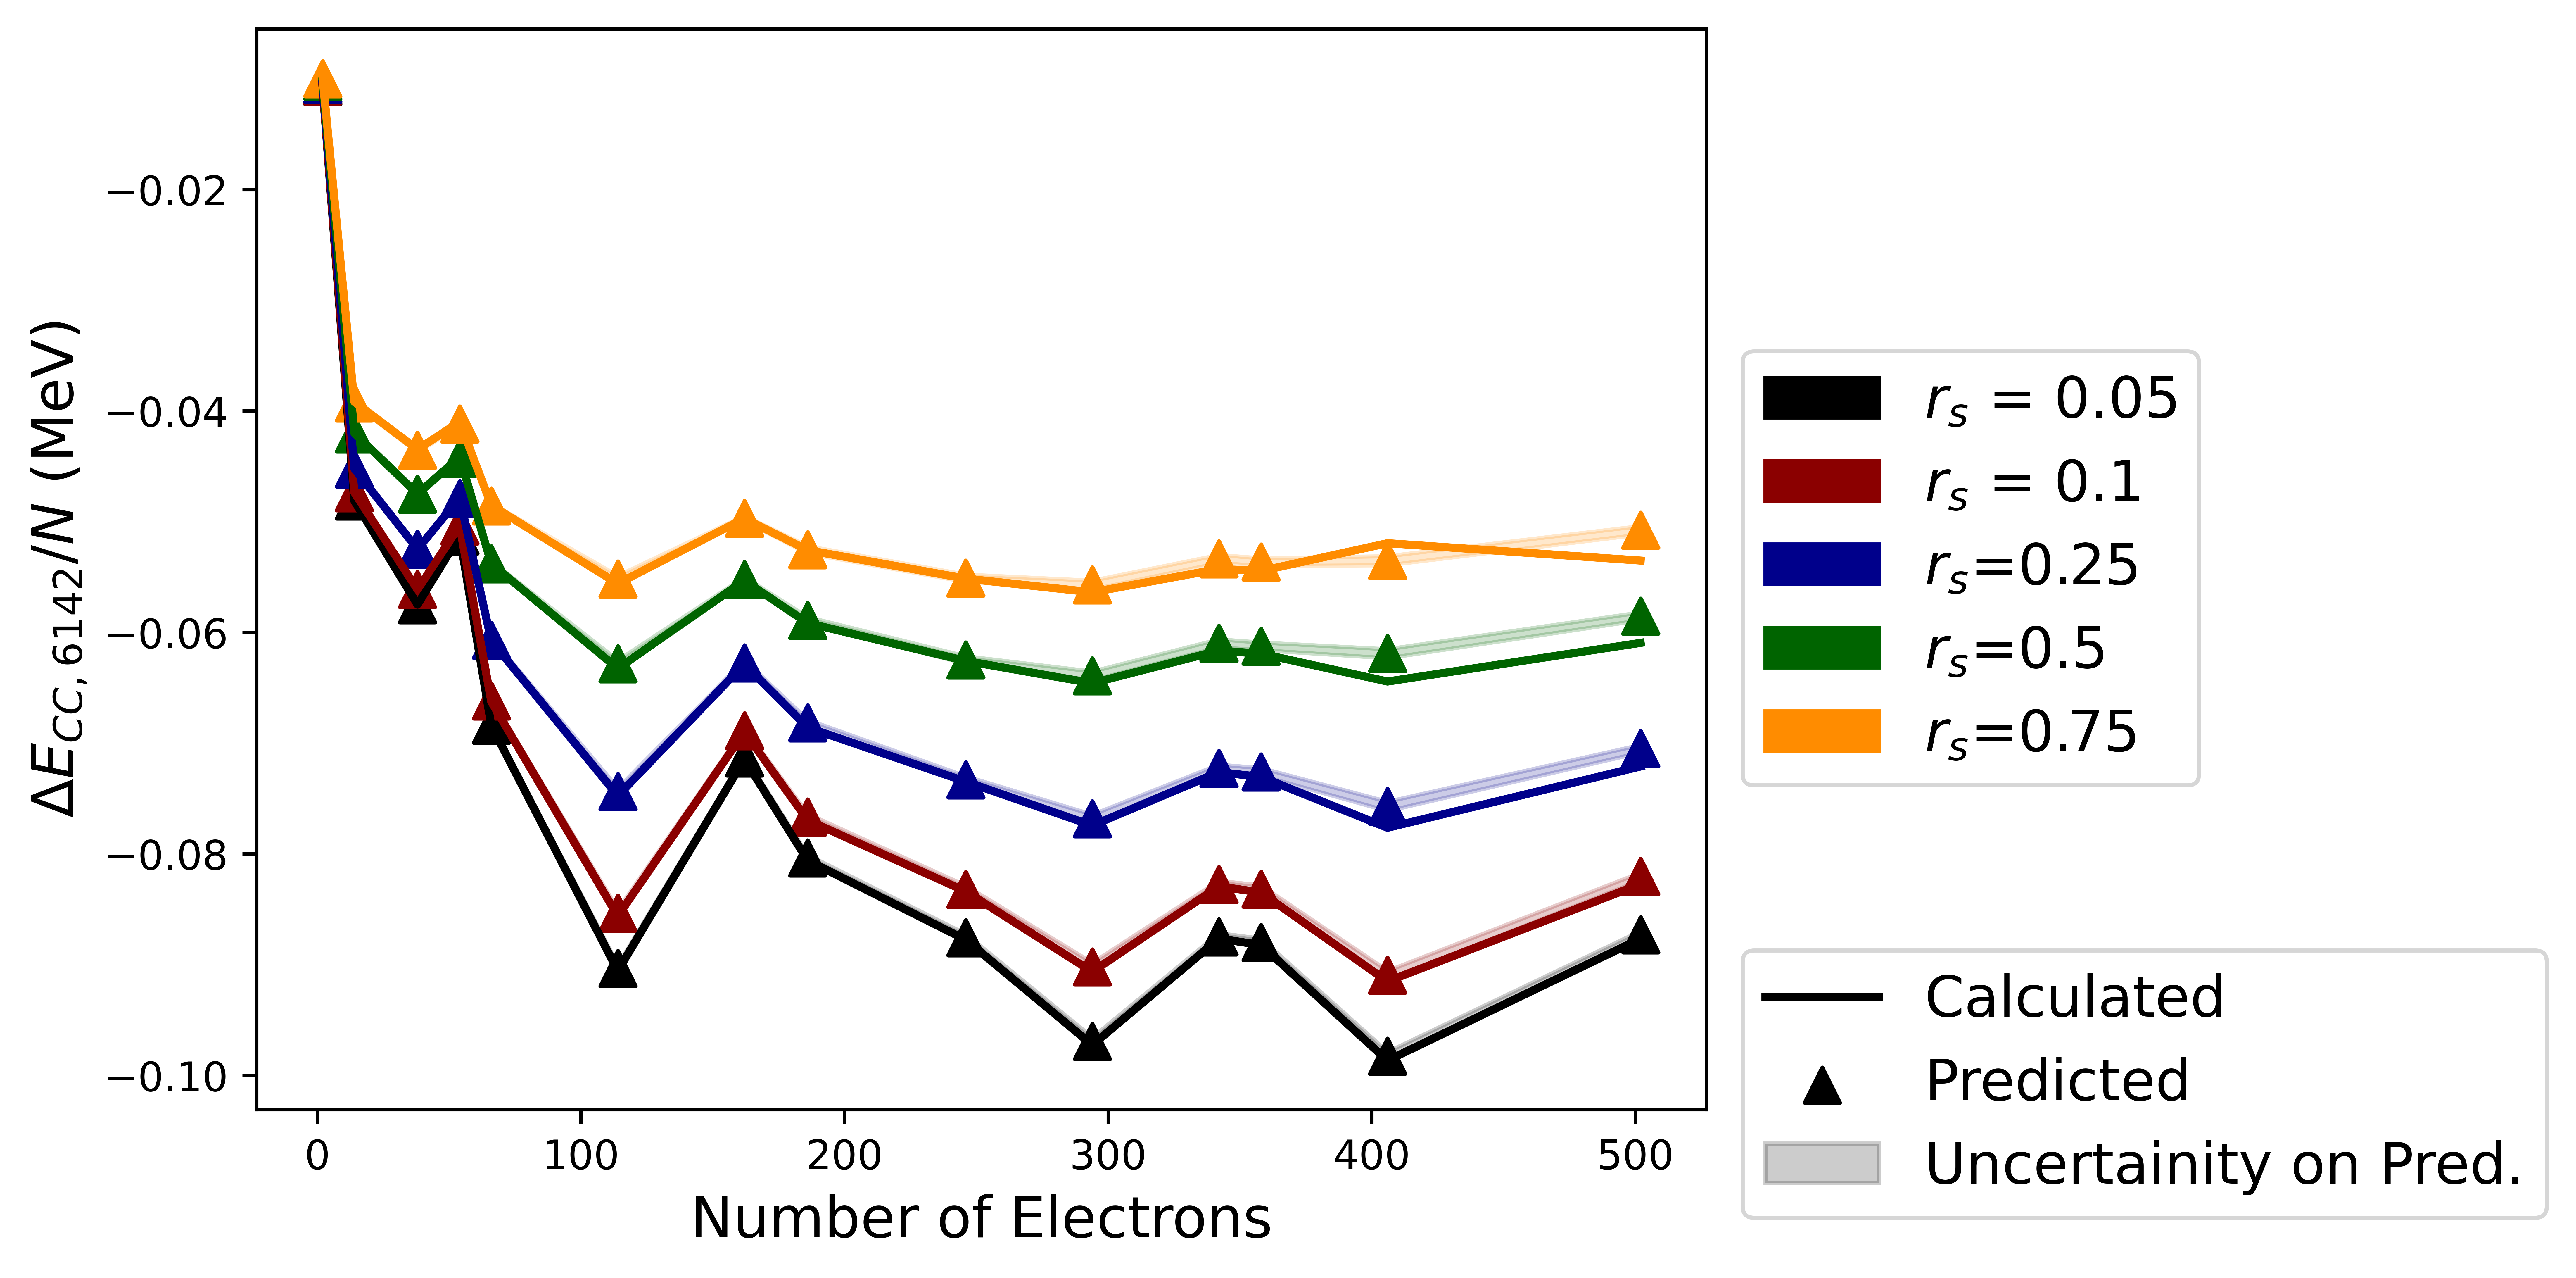
\includegraphics[scale=0.75]{Images/Chapter7/ElectronGas/BRR_EG_MSU_uncertainities-GP.png}
    \caption{The results of performing an SRE analysis with Gaussian processes to predict the converged correlation energies for the HEG at different values of N and $r_s$.  The correlation energies calculated at M = 6,142 are plotted with a solid line and are taken to be the true results, the SRE predictions are plotted with triangular markers, and the shaded region represents the uncertainty on the SRE predictions.}
    \label{fig:gp_16_points}
\end{figure}


As a final analysis with the SRE method on the HEG, we will again use GP as the machine learning algorithm but will reduce the number of training points from 16 to only 10. Here we will use data collected from 5 to 14 open shells, thus removing the six training points with the highest number of single-particle states (and thus the highest computational costs). Here we have also reduced the SRE sequence length to 1 as there are a few training points.

The results of performing this analysis are shown in Fig. \ref{fig:gp_10_points}, using the same plotting scheme as \ref{fig:gp_16_points}. The lower number of training points does lead to a higher average percent error of 1.16$\%$, but this is still a relatively low error, and it does appear, based on the results graph, that most of that error is concentrated in the last two points of the $r_s$ = 0.75 data set.

Next, we must point out the time savings we have gained by reducing the number of training points. When using 16 training points, the time savings is 88.99 node hours, which is not an insignificant amount of time saved. However, with only ten training points, and since the six training points we have removed have the most significant computational time, with this analysis, the amount of computational time saved is 224.43 node hours. That is equivalent to over a week in computational time saved for an error of only 1.16$\%$!

Finally, we justify using the Gaussian processes as the machine learning algorithm over Bayesian ridge regression when there is a small amount of training data. For example, suppose we were to perform this same analysis with Bayesian ridge regression, using ten training points and a sequence length of 1. In that case, the average percent error across all the correlation energies is 6.05$\%$, much higher than the 1.16$\%$ we see with GP. Thus, the GP algorithm works better with smaller data sets and will be the primary algorithm we will use in the next chapter to analyze the infinite nuclear matter, as no training set in that chapter will contain more than 10 points.

\begin{figure}
    \centering
    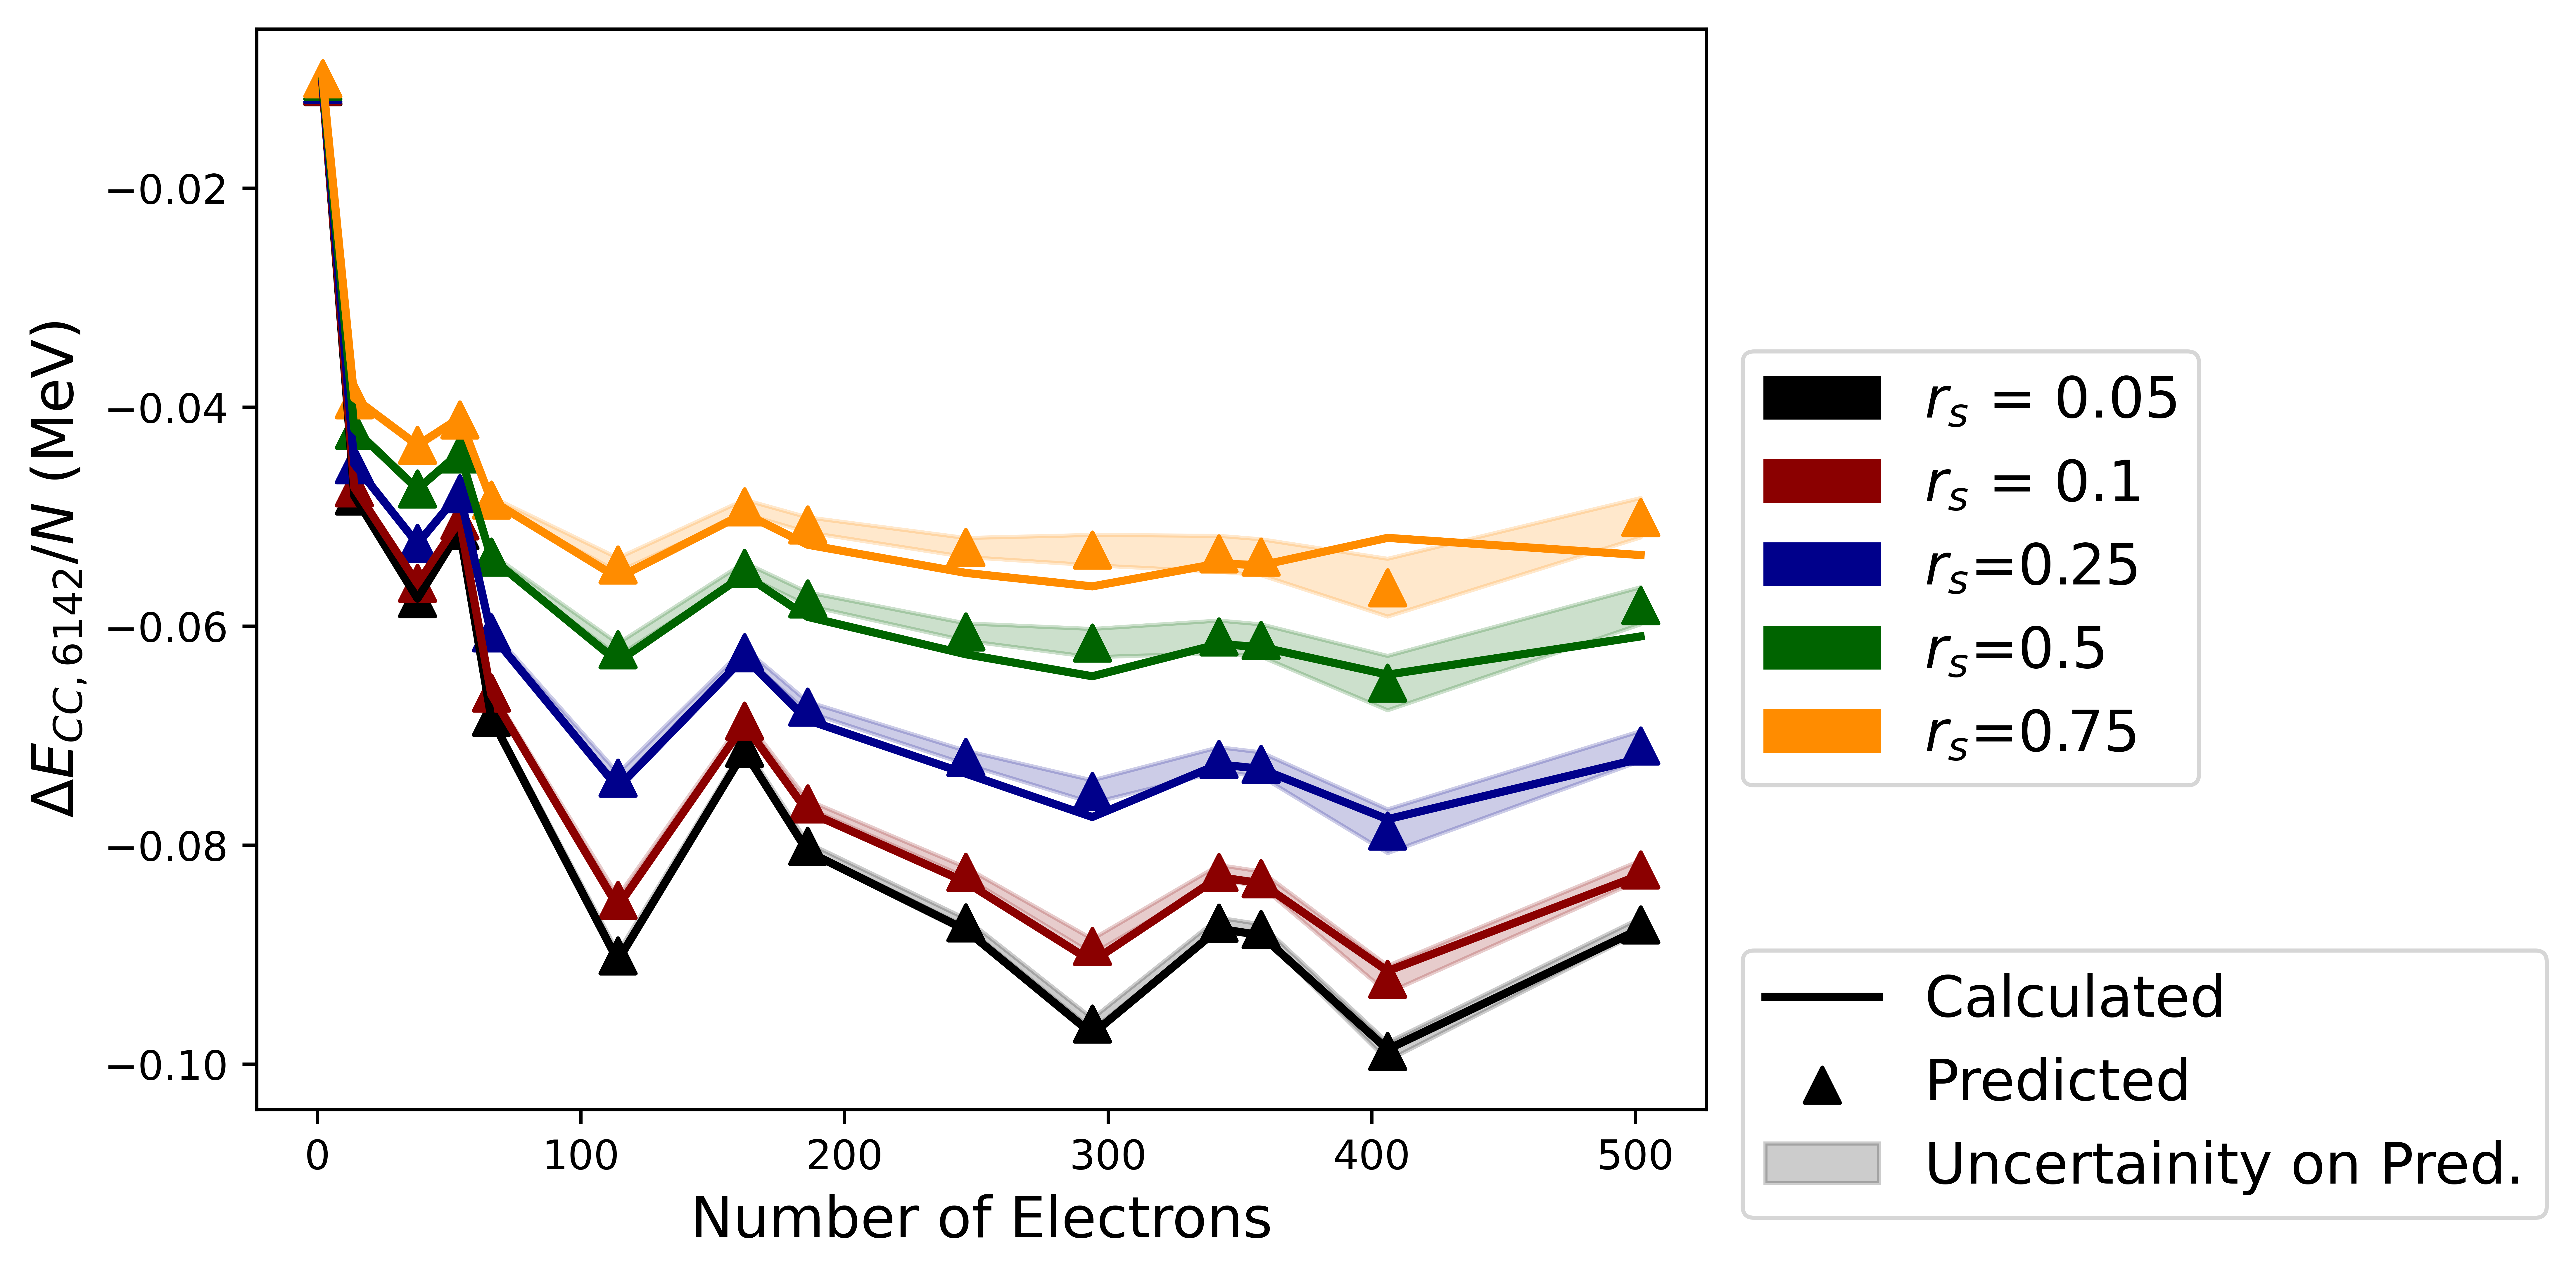
\includegraphics[scale=0.75]{Images/Chapter7/ElectronGas/BRR_EG_MSU_uncertainities_GP_2.png}
    \caption{The results of performing an SRE analysis with Gaussian processes to predict the converged correlation energies for the HEG at different values of N and $r_s$ and only ten training points.  The correlation energies calculated at M = 6,142 are plotted with a solid line and are taken to be the true results, the SRE predictions are plotted with triangular markers, and the shaded region represents the uncertainty on the SRE predictions.}
    \label{fig:gp_10_points}
\end{figure}        



    \section{Conclusion}
        %%% THESIS CONCLUSIONS %%%

% SRE as a valid extrapolation method
The sequential regression extrapolation (SRE) method developed here based on Bayesian regression algorithms is an accurate and valuable extrapolator for removing basis incompleteness errors from coupled cluster calculations of infinite matter systems. Furthermore, when the infinite matter system needs to be taken to the thermodynamic limit, it is possible to use SRE to perform this task. Since the SRE algorithm uses training data taken from calculations at small numbers of single-particle states to predict the correlation energy at many single-particle states, the SRE algorithm can offer significant time savings over performing fully converged correlation energy calculations. As shown in this thesis, using the SRE algorithm to save over 100 node hours in the calculations of just one correlation energy is possible. Furthermore, this huge time savings does come with a loss in the accuracy of performing the whole savings. However, the average percent error between the SRE prediction and the fully calculated result was typically less than 1$\%$, making it quite a slight difference compared to the large amount of computational time that has been saved.

% From the CCD vs. CCDT side
Furthermore, besides developing the SRE method, we also compared different methods of performing coupled cluster calculations of systems of infinite nuclear matter. First, we compared the results from two different interactions: the Minnesota potential, a toy interaction, and chiral NNLO potentials, which are much more realistic. By comparing these two, we learned that they differ quite significantly around densities of infinite nuclear matter that are similar to nuclear densities and that calculations containing NNLO potentials do take much longer to compute compared to a Minnesota potential applied to the same system. Furthermore, we could also compare the difference between the coupled cluster approximations CCD, CCDT-1, and CCD(T) on calculations of infinite matter systems. We found that the triples approximations give significant results when compared to the CCD approximation, so they are worth performing even though they provide an increase in computational time.

%% SIZE OF MACHINE LEARNING SYSTEM
Though it has been mentioned throughout this thesis, it is essential to emphasize the size of the training data sets used in this work. This work's most extensive training data set used only 16 training points, and the smallest training set used only 3 points. Some areas of physics could be faster to adopt machine learning because of the vast amount of training data that some machine learning algorithms require. However, this work has shown that accurate machine learning predictions can be made with very few training points, thus encouraging using machine learning as a tool in fields with small data sets.

%%% FUTURE WORKS %%%

\subsection*{Possible Future Works}
% Full triples and different proton fractions
A few notable future works stem directly from the work presented here. First, while we showed results from both the CCD< CCDT-1, and CCD(T) approximations, we did not have the capabilities to produce coupled cluster correlation energies using a complete CCDT calculation. This is mainly due to the high computational costs of a complete triple calculation ($O(M^8)$), but advancements, such as those made in Refs. Furthermore, ADD REFERENCES HERE are making this a much more achievable goal for the near future.

Additionally, while we only looked at pure neutron matter and symmetric nuclear matter here, there are other proton fractions of interest. If we want to model the equation of the state of nuclear matter thoroughly, then we need to be able to accurately predict the properties of neutron matter at proton fractions beyond just 0.0 and 0.5.

% PARAGRAPH ABOUT NOT BEING LIMITED TO INFINITE SYSTEMS
While truncating the number of particles in a calculation is limited to infinite matter and other large systems, truncations occur in every \textit{ab initio} many-body calculation. Basis truncation is especially common and occurs in almost every calculation except some simple toy models. The last part of this thesis will be dedicated to exploring some possible future applications of the SRE methodology which has been developed.

% PARAGRAPH ABOUT CC CALCULATIONS OF THE NUCLEUS
An extension of the work presented in this thesis is to apply the SRE method to remove basis incompleteness errors from coupled cluster calculations of nuclei. Though nuclei are finite systems and the number of nucleons in the system generally does not need to be truncated, the number of single-particle states is still truncated, leading to a need to extrapolate to an infinite model space \cite{Ref6}. This is especially true for heavy nuclei and nuclei that are weakly bound \cite{Ref6}. There are methods to perform these extrapolations on nuclei calculations, but when using the harmonic oscillator basis, which mixes the ultraviolet and infrared cutoffs, these extrapolation methods can fail \cite{Ref6}. Machine learning has been used to perform similar extrapolations (see Ref. \cite{Ref6}, \cite{Ref22}, \cite{Ref23}, for example), but these were performed with neural networks and thus incurred all of the problems that were experienced with neural networks in this thesis.

%% MBPT CALCULATIONS AND HIGHER ORDERS
Additionally, the SRE method has no reason to be restricted to only predicting CC energies using MBPT2 energies. Extending the SRE method to other many-body methods should also be possible. 

% PARAGRAPH ABOUT FCI
One of the most accurate yet restricted \textit{ab initio} many-body methods is full configuration interaction theory (FCI), which uses a variationally optimized linear combination of the full set of Slater determinants. FCI is used in nuclear physics and electronic-structure theory, but its complexity limits it to only the smallest of systems. The ground state energy, which FCI finds, is the lowest (variationally) and most accurate that can be achieved. If an infinite single particle basis is used, FCI produces the solutions to the Schr\"{o}dinger equation. However, due to computational limitations, FCI calculations must be performed with a finite basis, meaning they will fail to retrieve the total energy \cite{Ref1}. However, it is possible that SRE could be applied to FCI calculations using, for example, Hartree Fock calculations as the "fast method" to quickly and accurately extrapolate FCI results to the infinite basis limit, thus recovering the Schr\"{o}dinger equation results.

 % APPLICATIONS OUTSIDE OF NUCLEAR PHYSICS
While most of this thesis, except for the sections on the electron gas, have been devoted to nuclear physics applications, \textit{ab initio} many-body methods occur in many other fields besides nuclear physics. For example, coupled cluster theory, and other many-body methods, are prevalent in other fields of physics and quantum chemistry. Therefore, the development of the SRE method should improve calculations outside of the realm in which it was developed.

%%%%%%%%%%%%%%%%%%%%%%%%%%%%%%
%% CHAPTER: SRE
%%%%%%%%%%%%%%%%%%%%%%%%%%%%%%
\chapter{Sequential Regression Extrapolation (SRE)}
    %%%%%%%%%%%%%%%%%%%%%%%%%%%%%%
    %% Introduction and Methodology
    %%%%%%%%%%%%%%%%%%%%%%%%%%%%%%
    \section{Introduction to Methodology}
        \chapter*{Introduction}

%VMC methods pose a very attractive alternative to other more complex ways of finding the ground state energies of simple atoms and molecules, like configuration-interaction calculations. The price to be paid in exchange for this simplicity is the sensitivity to the trial wave functions that are used, a VMC algorithm is very sensitive to how these are constructed, so they are one of the most important aspects to be considered (in this work, given the simple nature of the atoms which we will be working with, it's not so important to worry about the quality of the trial wave functions because very simple and basic ones are more than enough to reproduce the actual results). It shouldn't be forgotten that it is a variational method, and this implies that finding the optimal set of variational parameters is going to be the most important part of the calculation itself because it would create a lot of problems if the search range for the parameters was illy defined and not close enough to the variational minimum, namely, the results would have a poor quality in this case. This means that the parameters need to be chosen very carefully, or a recursive search with decreasingly coarse spacing in the space of variational parameters is required if there is no deep knowledge about the system in question.

%Instead of evaluating a very complex multidimensional integral to compute the expectation value of an operator, like the hamiltonian in this case, a VMC calculation exploits the fact that the majority of the configuration space where the wave function belongs can be regarded as much less important than other parts, the values of the wave function are too small there and can be mostly ignored during the integration of the algorithm. To capitalize this, the Metropolis algorithm is added to the VMC method, as well as importance sampling and Gaussian Type Orbitals.

%\todo{motivasjon (QD i 2D og 3D + atomer -> fleksibel kode)}
%\subsubsection{Introducing the problem and the flexible solver}
Quantum mechanical systems are complex. As such creating a specific
program for each specific system is not a viable method of studying a
range of systems. We need to generalize. A generalized solver for
quantum mechanical systems must be written without any constraints to
specific properties any system may have. To achieve such a feat the
program is best implemented by the use of object orientation, creating
an easily expandable solver to which simple or complex systems may be
added. In this thesis the aim is to write a generalized variational
Monte Carlo solver which, by using object orientation, may handle a
wide range of quantum mechanical systems, such as confined electrons
in so-called quantum dots, atoms, and molecules.

%\subsubsection{Further introduction to the solver, the trial function, the slater determinant}
The variational Monte Carlo method poses an attractive way to solve
quantum mechanichal systems, compared to other more complex methods,
while also taking correlation factors into account, as opposed to the
Hartree-Fock method. The attractiveness of the variational Monte Carlo
method lies in the way it solves the multi-dimensional integrals
arising in the many-body quantum mechanical problem, which, as the
name implies, is by using the Monte Carlo method. In this thesis a
single so-called Slater determinant is used as an ansatz for the trial
wave function. This simplicity makes it easy to implement an efficient
and flexible program. It is however a compromise, yielding less
accurate results, but nevertheless good enough to study a variety of
systems.

%\subsubsection{Introducing the QD problem in 2 and 3 dimensions, and atoms. Tie to use of flexible code}
The solver presented in this thesis was initially made to solve simple
atomic systems, as a reference, and thereby expanding to molecules. To further
demonstrate the flexibility of the program, quantum dots are studied
in two and three dimensions. The reason for choosing quantum dots to
be studied is their simple structure, yet multitude of practical uses.


%\todo{hva jeg har gjort}
%\subsubsection{Introduce implementation of the code}


%\subsubsection{Short description of various tests done with QD and atoms}
The aim in this thesis is to demonstrate the flexibility of the
program by studying the system like atomic helium, beryllium and neon,
the helium and beryllium molecules, benchmarking ground state energies
against existing references, and studying their one-body densities. Furthermore
quantum dots consisting of up to 56 electrons will be studied in a
similar manner, and their frequency will be varied.  With a lower
frequency the quantum dots will implicity have a higher correlation,
and studying correlations are of great importance when using more
elaborate methods than for example the simple Hartree-Fock method.

Ground states of atoms and molecules are compared to experimental
results, which should be close to the exact results, offering a good
test of the accuracy of the variational Monte Carlo method and the
solver created. Because of the popularity of quantum dots several
master students have studied them, each with different methods. This
provides a wide range of references to which ground state energies may
be compared, which should give further insight to the accuracy of the
solver.

%\todo{oppgavens struktur}
%\subsubsection{Chapter by chapter}
The thesis is structured in two parts: a theory part, and a results part. A brief description of the chapters is given below.
\begin{itemize}
	\item In the first chapter a brief introduction to scientific computing is given. In it different types of programming languages will be described, and we will give an introduction to object-oriented programming. This is important because object-oriented programming is used to create a generalized solver. A summary of message passing interface, used to parallelize the computations, is also given.  
	\item The second chapter aims to give an overview of a more basic solution method, the Hartree-Fock method. It also describes other methods derived from the Hartree-Fock method, so-called post Hartree-Fock methods. The Hartree-Fock method can be used as a convenient test for a more simplified variational Monte Carlo program, and some of the post Hartree-Fock methods are used in computations of references when ground state energies computed by the solver is benchmarked.
	\item Next the variational Monte Carlo method is explained with details around ways of optimization, like the Metropolis algorithm and importance sampling. Details about how to calculate the Slater determinant efficiently and other measures to further optimize the solver are also given. Then the process of blocking to get an accurate estimate of the error is explained.
	\item In the fourth chapter the modelled systems are described. How quantum dots are modelled in two and three dimensions is described, then a brief descrition of how each of the atomic systems are modelled is given. A way to replace the Slater type orbitals with gaussian type orbitals is also described.
	\item In the final chapter of the first part we look at how the solver is structured, and how the variational Monte Carlo method is implemented using object-orientation.
	\item With the theory in place we look at the results from calculations with the variational Monte Carlo solver created. The program is benchmarked to test the optimizations and also to see how well it scales with an increasing number of processors used. The systems are benchmarked against reference ground state energies, and one-body densities are calculated, which can give insight into the structure of the systems. 
	\item Finally a conclusion is given with final remarks.
\end{itemize}


%`God does not play dice' Einstein said \todo{ref}, refuting the theory that quantum mechanical systems are governed by probability. However, as it turns out, we may, to solve them.


    %%%%%%%%%%%%%%%%%%%%%%%%%%%%%%
    %% Formulation
    %%%%%%%%%%%%%%%%%%%%%%%%%%%%%%
    \section{Formulation}
        As discussed in the previous chapter, supervised machine learning algorithms require label training data, meaning that both x and y components exist. Therefore, a supervised machine learning algorithm learns to approximate a function, f, during its training process such that f(x) = y for every value of x in the data set.  

%% Why the traditional way of training makes a bad extrapolator
However, supervised machine learning algorithms tend to fail when asked to make predictions outside their training range (for example, see Ref. \cite{Ref6}). Put another way, supervised machine learning algorithms tend to make more extrapolators and are thus not used for extrapolation applications. However, one type of supervised machine learning performed well with extrapolations; in fact, it was designed to make extrapolations on time series data. This algorithm is the recurrent neural network discussed in the last section. RNNs perform very well on extrapolations as their design inherently gives them some "memory" of previous data that they can use to predict new data.

%% neural network drawbacks
While RNNS may be a good choice for performing time series analysis and extrapolations, they have some significant drawbacks when applying them to \textit{ab initio} data sets. First, RNNs, like all neural networks, require much training data to make accurate predictions and avoid overfitting. While this is not a problem for many applications of neural networks, this is a significant drawback when applying any neural network to \textit{ab initio} data sets. Since each new point in an \textit{ab initio} data set can represent significant computational time and resource investment, these data sets are usually relatively small, especially by neural network standards \cite{Ref6}. One way around this is to use an interpolation algorithm to increase the size of the data set artificially, but this represents an additional step in the workflow and possibly an additional source of error in the analysis \cite{Ref6}. Thus in this work, we want to avoid using interpolation as much as possible.  

Secondly, due to how their weights are initialized, neural networks are inherently random \cite{Ref6}. This means a neural network, including RNNs, will produce slightly different results each time it is trained, even when the same training data is used. The irreproducibility is a significant drawback when using neural networks to predict physical values. Additionally, the uncertainty of a neural network's prediction is an open research question. 

Finally, as mentioned in the previous chapter, neural networks generally have a large number of hyperparameters, including the number of hidden layers, the number of neurons per hidden layer, and the activation function, among many others. This leads to complicated and long tuning processes, dramatically increasing the runtime needed to perform an ML analysis.

%% time series formatting with regression algorithms: SRE
While RNNs are not a good choice of a machine learning algorithm for this application, we can take inspiration from them and create a machine learning algorithm that can. A standard machine learning algorithm is trained to take a point from the training set, $x_i$, and match it to its corresponding y values, $y_i$. Thus training a standard machine learning algorithm has the following relations to be learned:

\begin{equation}
    f_{ML}(x_1) = y_1, f_{ML}(x_2) = y_2, ... .
\end{equation}

While this training pattern makes many supervised machine learning algorithms excellent at matching new inputs to the correct output, they typically only perform well in the range of data encompassed by the training data.

However, there is a way to train RNNs around this problem. This training pattern is typically used when RNNs perform time-series analysis, which is common in the financial industry. Instead of learning the relationship between the x and y components of the data set, a time-series data formatting teaches the RNN to learn the pattern between a sequence of y values and the next y value in the training data. The training points in this form will look as follows:

\begin{equation}
    f_{RNN}(y_{k-3}, y_{k-2}, y_{k-1}) = y_k,
\end{equation}

making the RNN much better at extrapolating because it is trained to predict the next value in a sequence. Note that the sequence length in the inputs could be of any length, thus adding another hyperparameter.

The drawback of this form of training here is that the data must be sequential (have an order to it), and the data must be evenly spaced regarding the dependent variables. Additionally, since the RNN only sees the y component of the data, it may lose the information encoded in the x component. However, an RNN trained in this manner is an extremely powerful extrapolator.

Nevertheless, as explained earlier in this section, there are several drawbacks to using RNNs in this application. However, we can combine the training style of an RNN with a simpler machine-learning algorithm to make a more straightforward but still powerful extrapolator. Furthermore, since none of the data in this thesis is time-dependent, instead of calling this style of formatting the data a time series, we will call it sequential formatting, as the data must be arranged sequentially. This gives rise to the name of the machine learning algorithm we are building to extrapolate many-body data sets, sequential regression extrapolation (SRE); so named because it combines sequential data formatting with a regression algorithm to create an extrapolator that can make predictions from small data sets. Thus we will train a regression algorithm using the following format:

\begin{equation}
    f_{R}(y_{k-3}, y_{k-2}, y_{k-1}) = y_k.
\end{equation}

The length of the input, now known as the SRE sequence length, can be any length. However, the larger the sequence length is, the fewer total data points present once the data has been formatted, so there is a balancing act between choosing a sequence length long enough to encode the sequential patterns in the data but not so long that there are very few points remaining after the formatting.

Now that we have developed the algorithm generally, we can apply it to remove the basis incompleteness and finite size errors arising from many-body calculations of infinite matter systems. The remainder of this section will develop the specific SRE formulism to remove these errors.




   
        %%%%%%%%%%%%%%%%%%%%%%%%%%%%%%
        %% wrt m
        %%%%%%%%%%%%%%%%%%%%%%%%%%%%%%
        \section{CCD Extrapolations With Respect to Number of Single Particle States}
            This section describes the SRE formulation to remove the basis incompleteness errors from CCD calculations of infinite matter. 

Both the $\Delta E_{CC}$ and $\Delta E_{MBPT}$ converge as M increases. In that case, there must be a large value of M where their ratio becomes a constant:


\begin{equation}
\frac{\Delta E_{CC,Large\ M}}{\Delta E_{MBPT,Large\ M}} \longrightarrow constant.
\end{equation}

One of the machine learning algorithms described in the previous chapter will be used to find this constant value using only data collected at low values of M, where the ratio still needs to be converged. $\Delta E_{CC}$ and $\Delta E_{MBPT}$ are calculated for the training data set generated at small values of M. The exact values of M will depend on the value of N and the system in the calculations. However, the largest value of M used across all training data in this thesis is 2,090 single-particle states. For each data set (constant N and $\rho_0$/$r_s$), the training data for the regression algorithm was created by dividing $\Delta E_{CC}$ by $\Delta E_{MBPT}$ at the exact value of M.

\begin{equation}
y =\frac{\Delta E_{CC,M}}{\Delta E_{MBPT,M}} = \frac{\Delta E_{CC,M_1}}{\Delta E_{MBPT,M_1}}, \frac{\Delta E_{CC,M_2}}{\Delta E_{MBPT,M_2}}, \frac{\Delta E_{CC,M_3}}{\Delta E_{MBPT,M_3}}, ...
\end{equation}

Next, the machine learning algorithm, $f_R$, is trained on this data set using the SRE formulation developed earlier in this chapter. The sequence length shown here is three data points, but depending on the analysis being done, it could range from 1 to 3. We are adding this hyperparameter into the analysis, whose value will have to be set, but in general, we want a smaller sequence length if there is less training data. 

\begin{equation}
f_{R}(\frac{\Delta E_{CC,k-3}}{\Delta E_{MBPT,k-3}},\frac{\Delta E_{CC,k-2}}{\Delta E_{MBPT,k-2}}, \frac{\Delta E_{CC,k-1}}{\Delta E_{MBPT,k-1}}) = \frac{\Delta E_{CC,k}}{\Delta E_{MBPT,k}}
\end{equation}

The SRE algorithm is then used to extrapolate this data set to many points until the ratio of correlation energies has converged. This value can then be taken as the slope of the graph created with $\Delta E_{CC}$ plotted as a function of $\Delta E_{MBPT}$.

\begin{equation}
\lim_{k\to\infty} \frac{\Delta E_{CC,k}}{\Delta E_{MBPT,k}} = slope = m
\end{equation}

Finally, $\Delta E_{MBPT, Large\ M}$  is generated, a process that takes less than one second (not including the time to generate the matrix elements). $\Delta E_{MBPT, Large\ M}$ is multiplied by the slope, m, to approximate $\Delta E_{CC, Large\ M}$.

\begin{equation}
m\Delta E_{MBPT,Large\ M} \approx \Delta E_{CC,Large\ M}
\end{equation}

Due to convergence, the number of single-particle states used to calculate the large M data sets will vary depending on the system. For example, for the HEG, M = 6,142 (70 total shells) is used because the CCD correlation energies were confirmed to be converged at this point across all values of N and r$_s$ tested. It is important to note that the data sets used to train a machine learning algorithm in this work consist of 3-16 points each, making these data sets some of the smallest used in physics applications of machine learning. Many machine learning algorithms need more points to be accurately trained, even up to 1-2 orders of magnitude more, as with some neural networks. For example, the ML-based process shown in Ref. \cite{Ref7} can generate accurate molecular CCD correlation energies using only 12 data points with kernel ridge regression and a training process based on MP2 amplitudes. However, the MP2 amplitudes used in the training data have a very high dimensionality which can increase the time needed for training. Some other studies designed machine learning algorithms to use small data sets but still needed around 100 data points, if not more (see Ref. \cite{Ref17} for example) and are usually artificially extended with interpolation (for example, see \cite{Ref6}. 

It is also of note that machine learning is typically only used to make extrapolations in exceptional cases such as recurrent neural networks. When asked to make predictions outside their training range, many machine learning algorithms could improve. However, it will be shown that SRE can make accurate extrapolations using only a small training set, making it a unique machine-learning algorithm. There is, however, a drawback to the SRE method. Since it relies only on the y component of the training data set, it assumes that the data is evenly spaced with respect to the x variable and can only make predictions at the same spacing. This works well for this application since "evenly spaced" means a calculation at every closed shell of unoccupied states, and extrapolations are made until the result converges (the exact x value where this occurs is not essential for this study). However, this limitation does mean that the SRE method is only suitable for some applications.

The SRE method must meet two metrics to be a helpful extrapolator. First, the total time to generate the training data, train the SRE algorithm, and predict the converged correlation energy must be less than the time to calculate the correlation energy at M = 6142. Secondly, the accuracy between the predicted and calculated converged correlation energies must be high, preferably with a percent error between the two data sets of less than 2$\%$.

\subsubsection* {Error Analysis on Prediction}

The prediction has a measurable uncertainty since Bayesian methods calculate the slope, m. This can be transferred to an uncertainty on the predicted converged CCD correlation energy using the following scheme. Given that the converged CCD correlation energy is:

\begin{equation}
    \Delta E_{CC} = m\Delta E_{MBPT},
\end{equation}

then we can relate the uncertainties on all three quantities using equation Eq. \ref{uncertainity1}.  In Eq. \label{uncertainity1}, $\delta x$ refers to the uncertainty associated with quantity x.

\begin{equation}\label{uncertainity1}
    \frac{\delta \Delta E_{CC}}{\Delta E_{CC}} = \frac{\delta \Delta E_{MBPT}}{\Delta E_{MBPT}} + \frac{\delta m}{m}
\end{equation}

We will also assume that the uncertainty in the calculation of the MBPT2 correlation energy is 0, so \ref{uncertainity1} simplifies to:

\begin{equation}\label{uncertainity2}
    \frac{\delta \Delta E_{CC}}{\Delta E_{CC}} = \frac{\delta m}{m}.
\end{equation}

Now, Eq. \ref{uncertainity2} is solved for $\delta \Delta E_{CC}$, or the uncertainty on the predicted converged CCD correlation energy, yielding:

\begin{equation}
    \delta \Delta E_{CC} = \frac{\Delta E_{CC}}{m}\delta m.
\end{equation}

However, this can be simplified using the following:

\begin{equation}
    \Delta E_{CC} = m\Delta E_{MBPT} \longrightarrow \Delta E_{MBPT} = \frac{\Delta E_{CC}}{m},
\end{equation}

yielding as a final equation for the CCD correlation energy uncertainty:

\begin{equation}\label{uncertainity3}
    \delta \Delta E_{CC} = \Delta E_{MBPT}\delta m.
\end{equation}

Finally, to present the results as the correlation energy per particle, as is typically done with infinite nuclear matter calculations, the uncertainty in the predicted converged CCD correlation energy can be found by dividing both sides of Eq. \ref{uncertainity3} by N.

\begin{equation}
    \delta (\frac{\Delta E_{CC}}{N} = \frac{\Delta E_{MBPT}}{N}\delta m
\end{equation}

        %%%%%%%%%%%%%%%%%%%%%%%%%%%%%%
        %% wrt n
        %%%%%%%%%%%%%%%%%%%%%%%%%%%%%%
        \section{CCD Extrapolations With Respect to Number of Particles}
            Removing the finite size error from truncating the number of particles in the system will be similar to removing the basis incompleteness error.  We will start with a data set that is created by dividing the converged CCD correlation energies by the number of particles in the system for small values of N, resulting in:

\begin{equation}
    y = \frac{\Delta E_{CCD}^{N_k}}{N_k} = \frac{\Delta E_{CCD}^{N_1}}{N_1}, \frac{\Delta E_{CCD}^{N_2}}{N_2}, ... .
\end{equation}

Then we will train a machine learning algorithm using the sequential formatting developed in this last section on the data set we have created.

\begin{equation}
    f_R(\frac{\Delta E_{CCD}^{N_{k-3}}}{N_{k-3}}, \frac{\Delta E_{CCD}^{N_{k-2}}}{N_{k-2}}, \frac{\Delta E_{CCD}^{N_{k-1}}}{N_{k-1}}) = \frac{\Delta E_{CCD}^{N_{k}}}{N_{k}}
\end{equation}

The final step is to use the trained machine learning algorithm to extrapolate this ratio until convergence, resulting in the CCD correlation energy in the thermodynamic limit.  Thus, we have:

\begin{equation}
    \lim_{k\to\infty} = \lim_{k\to\infty} = \Delta E_{CCD}^\infty,
\end{equation}

where $\Delta E_{CCD}^\infty$ is the CCD correlation energy per particle in the thermodynamic limit.  Additionally, since the prediction the machine learning algorithm makes is the result we are looking for, the uncertainty of that prediction does not need to be modified.

        %%%%%%%%%%%%%%%%%%%%%%%%%%%%%%
        %% wrt m
        %%%%%%%%%%%%%%%%%%%%%%%%%%%%%%
        \section{CCDT Extrapolations With Respect to Number of Single Particle States}
            For removing the basis incompleteness errors from calculations using the approximative triples methods, we will use the same method developed for removing the basis incompleteness errors from CCD calculations.  Even though the MPBT2 correlation energies are still at a comparatively lower level of approximation than the CCDT approximations, the SRE methods will still extrapolate well because both MBPT2 and CCDT converge as the value of M increases, and both MBPT2 and CCDT converge at roughly the same rate.  So, fortunately, CCD and CCDT correlation energies can be predicted with the same methods.

However, we will not perform extrapolations to the thermodynamic limit for the approximative triples calculations because we will use system sizes that already reduce the finite size effects.  This will be explained in greater detail in Chapter 8.

        \section{Conclusion}
            %%% THESIS CONCLUSIONS %%%

% SRE as a valid extrapolation method
The sequential regression extrapolation (SRE) method developed here based on Bayesian regression algorithms is an accurate and valuable extrapolator for removing basis incompleteness errors from coupled cluster calculations of infinite matter systems. Furthermore, when the infinite matter system needs to be taken to the thermodynamic limit, it is possible to use SRE to perform this task. Since the SRE algorithm uses training data taken from calculations at small numbers of single-particle states to predict the correlation energy at many single-particle states, the SRE algorithm can offer significant time savings over performing fully converged correlation energy calculations. As shown in this thesis, using the SRE algorithm to save over 100 node hours in the calculations of just one correlation energy is possible. Furthermore, this huge time savings does come with a loss in the accuracy of performing the whole savings. However, the average percent error between the SRE prediction and the fully calculated result was typically less than 1$\%$, making it quite a slight difference compared to the large amount of computational time that has been saved.

% From the CCD vs. CCDT side
Furthermore, besides developing the SRE method, we also compared different methods of performing coupled cluster calculations of systems of infinite nuclear matter. First, we compared the results from two different interactions: the Minnesota potential, a toy interaction, and chiral NNLO potentials, which are much more realistic. By comparing these two, we learned that they differ quite significantly around densities of infinite nuclear matter that are similar to nuclear densities and that calculations containing NNLO potentials do take much longer to compute compared to a Minnesota potential applied to the same system. Furthermore, we could also compare the difference between the coupled cluster approximations CCD, CCDT-1, and CCD(T) on calculations of infinite matter systems. We found that the triples approximations give significant results when compared to the CCD approximation, so they are worth performing even though they provide an increase in computational time.

%% SIZE OF MACHINE LEARNING SYSTEM
Though it has been mentioned throughout this thesis, it is essential to emphasize the size of the training data sets used in this work. This work's most extensive training data set used only 16 training points, and the smallest training set used only 3 points. Some areas of physics could be faster to adopt machine learning because of the vast amount of training data that some machine learning algorithms require. However, this work has shown that accurate machine learning predictions can be made with very few training points, thus encouraging using machine learning as a tool in fields with small data sets.

%%% FUTURE WORKS %%%

\subsection*{Possible Future Works}
% Full triples and different proton fractions
A few notable future works stem directly from the work presented here. First, while we showed results from both the CCD< CCDT-1, and CCD(T) approximations, we did not have the capabilities to produce coupled cluster correlation energies using a complete CCDT calculation. This is mainly due to the high computational costs of a complete triple calculation ($O(M^8)$), but advancements, such as those made in Refs. Furthermore, ADD REFERENCES HERE are making this a much more achievable goal for the near future.

Additionally, while we only looked at pure neutron matter and symmetric nuclear matter here, there are other proton fractions of interest. If we want to model the equation of the state of nuclear matter thoroughly, then we need to be able to accurately predict the properties of neutron matter at proton fractions beyond just 0.0 and 0.5.

% PARAGRAPH ABOUT NOT BEING LIMITED TO INFINITE SYSTEMS
While truncating the number of particles in a calculation is limited to infinite matter and other large systems, truncations occur in every \textit{ab initio} many-body calculation. Basis truncation is especially common and occurs in almost every calculation except some simple toy models. The last part of this thesis will be dedicated to exploring some possible future applications of the SRE methodology which has been developed.

% PARAGRAPH ABOUT CC CALCULATIONS OF THE NUCLEUS
An extension of the work presented in this thesis is to apply the SRE method to remove basis incompleteness errors from coupled cluster calculations of nuclei. Though nuclei are finite systems and the number of nucleons in the system generally does not need to be truncated, the number of single-particle states is still truncated, leading to a need to extrapolate to an infinite model space \cite{Ref6}. This is especially true for heavy nuclei and nuclei that are weakly bound \cite{Ref6}. There are methods to perform these extrapolations on nuclei calculations, but when using the harmonic oscillator basis, which mixes the ultraviolet and infrared cutoffs, these extrapolation methods can fail \cite{Ref6}. Machine learning has been used to perform similar extrapolations (see Ref. \cite{Ref6}, \cite{Ref22}, \cite{Ref23}, for example), but these were performed with neural networks and thus incurred all of the problems that were experienced with neural networks in this thesis.

%% MBPT CALCULATIONS AND HIGHER ORDERS
Additionally, the SRE method has no reason to be restricted to only predicting CC energies using MBPT2 energies. Extending the SRE method to other many-body methods should also be possible. 

% PARAGRAPH ABOUT FCI
One of the most accurate yet restricted \textit{ab initio} many-body methods is full configuration interaction theory (FCI), which uses a variationally optimized linear combination of the full set of Slater determinants. FCI is used in nuclear physics and electronic-structure theory, but its complexity limits it to only the smallest of systems. The ground state energy, which FCI finds, is the lowest (variationally) and most accurate that can be achieved. If an infinite single particle basis is used, FCI produces the solutions to the Schr\"{o}dinger equation. However, due to computational limitations, FCI calculations must be performed with a finite basis, meaning they will fail to retrieve the total energy \cite{Ref1}. However, it is possible that SRE could be applied to FCI calculations using, for example, Hartree Fock calculations as the "fast method" to quickly and accurately extrapolate FCI results to the infinite basis limit, thus recovering the Schr\"{o}dinger equation results.

 % APPLICATIONS OUTSIDE OF NUCLEAR PHYSICS
While most of this thesis, except for the sections on the electron gas, have been devoted to nuclear physics applications, \textit{ab initio} many-body methods occur in many other fields besides nuclear physics. For example, coupled cluster theory, and other many-body methods, are prevalent in other fields of physics and quantum chemistry. Therefore, the development of the SRE method should improve calculations outside of the realm in which it was developed.


%%%%%%%%%%%%%%%%%%%%%%%%%%%%%%
%% CHAPTER: THE HOMOGENEOUS ELECTRON GAS RESULTS
%%%%%%%%%%%%%%%%%%%%%%%%%%%%%%
\chapter{The Homogeneous Electron Gas Results}
    %%%%%%%%%%%%%%%%%%%%%%%%%%%%%%
    %% Three-Dimensional Electron Gas
    %%%%%%%%%%%%%%%%%%%%%%%%%%%%%%
    %% NEED FURTHER INTRODUCTION
The first infinite matter system we will analyze with the SRE method is the homogeneous electron gas (HEG), described in Chapter 4. The HEG, as one of the simpler infinite matter systems, is an excellent sandbox to fully develop the SRE method described in the last chapter.



Fig. \ref{increase_m} shows the results of computing the CCD correlation per energy for a HEG with $r_s$ = 0.5 at various numbers of electrons and with four different numbers of single-particle states. We can see that the calculation of $\Delta E_{CC}$ depends heavily on the number of single-particle states in the system, and we can begin to see that the correlation energy converges as the number of single-particle states in the system increases. The calculations performed with only 514 single-particle states (or 15 shells) are the least accurate of the four plots in Fig. \ref{increase_m} since they are performed with the fewest single-particle states. On the other hand, the calculations performed with 6,142 single-particle states (or 70 shells in total) are the most accurate of the four plots, and in fact, the convergence of $\Delta E_{CC}$ has been confirmed at this point. However, it is not always feasible to perform the calculations at this high number of single-particle states due to the associated high computational time and resource requirements.

\begin{figure}
    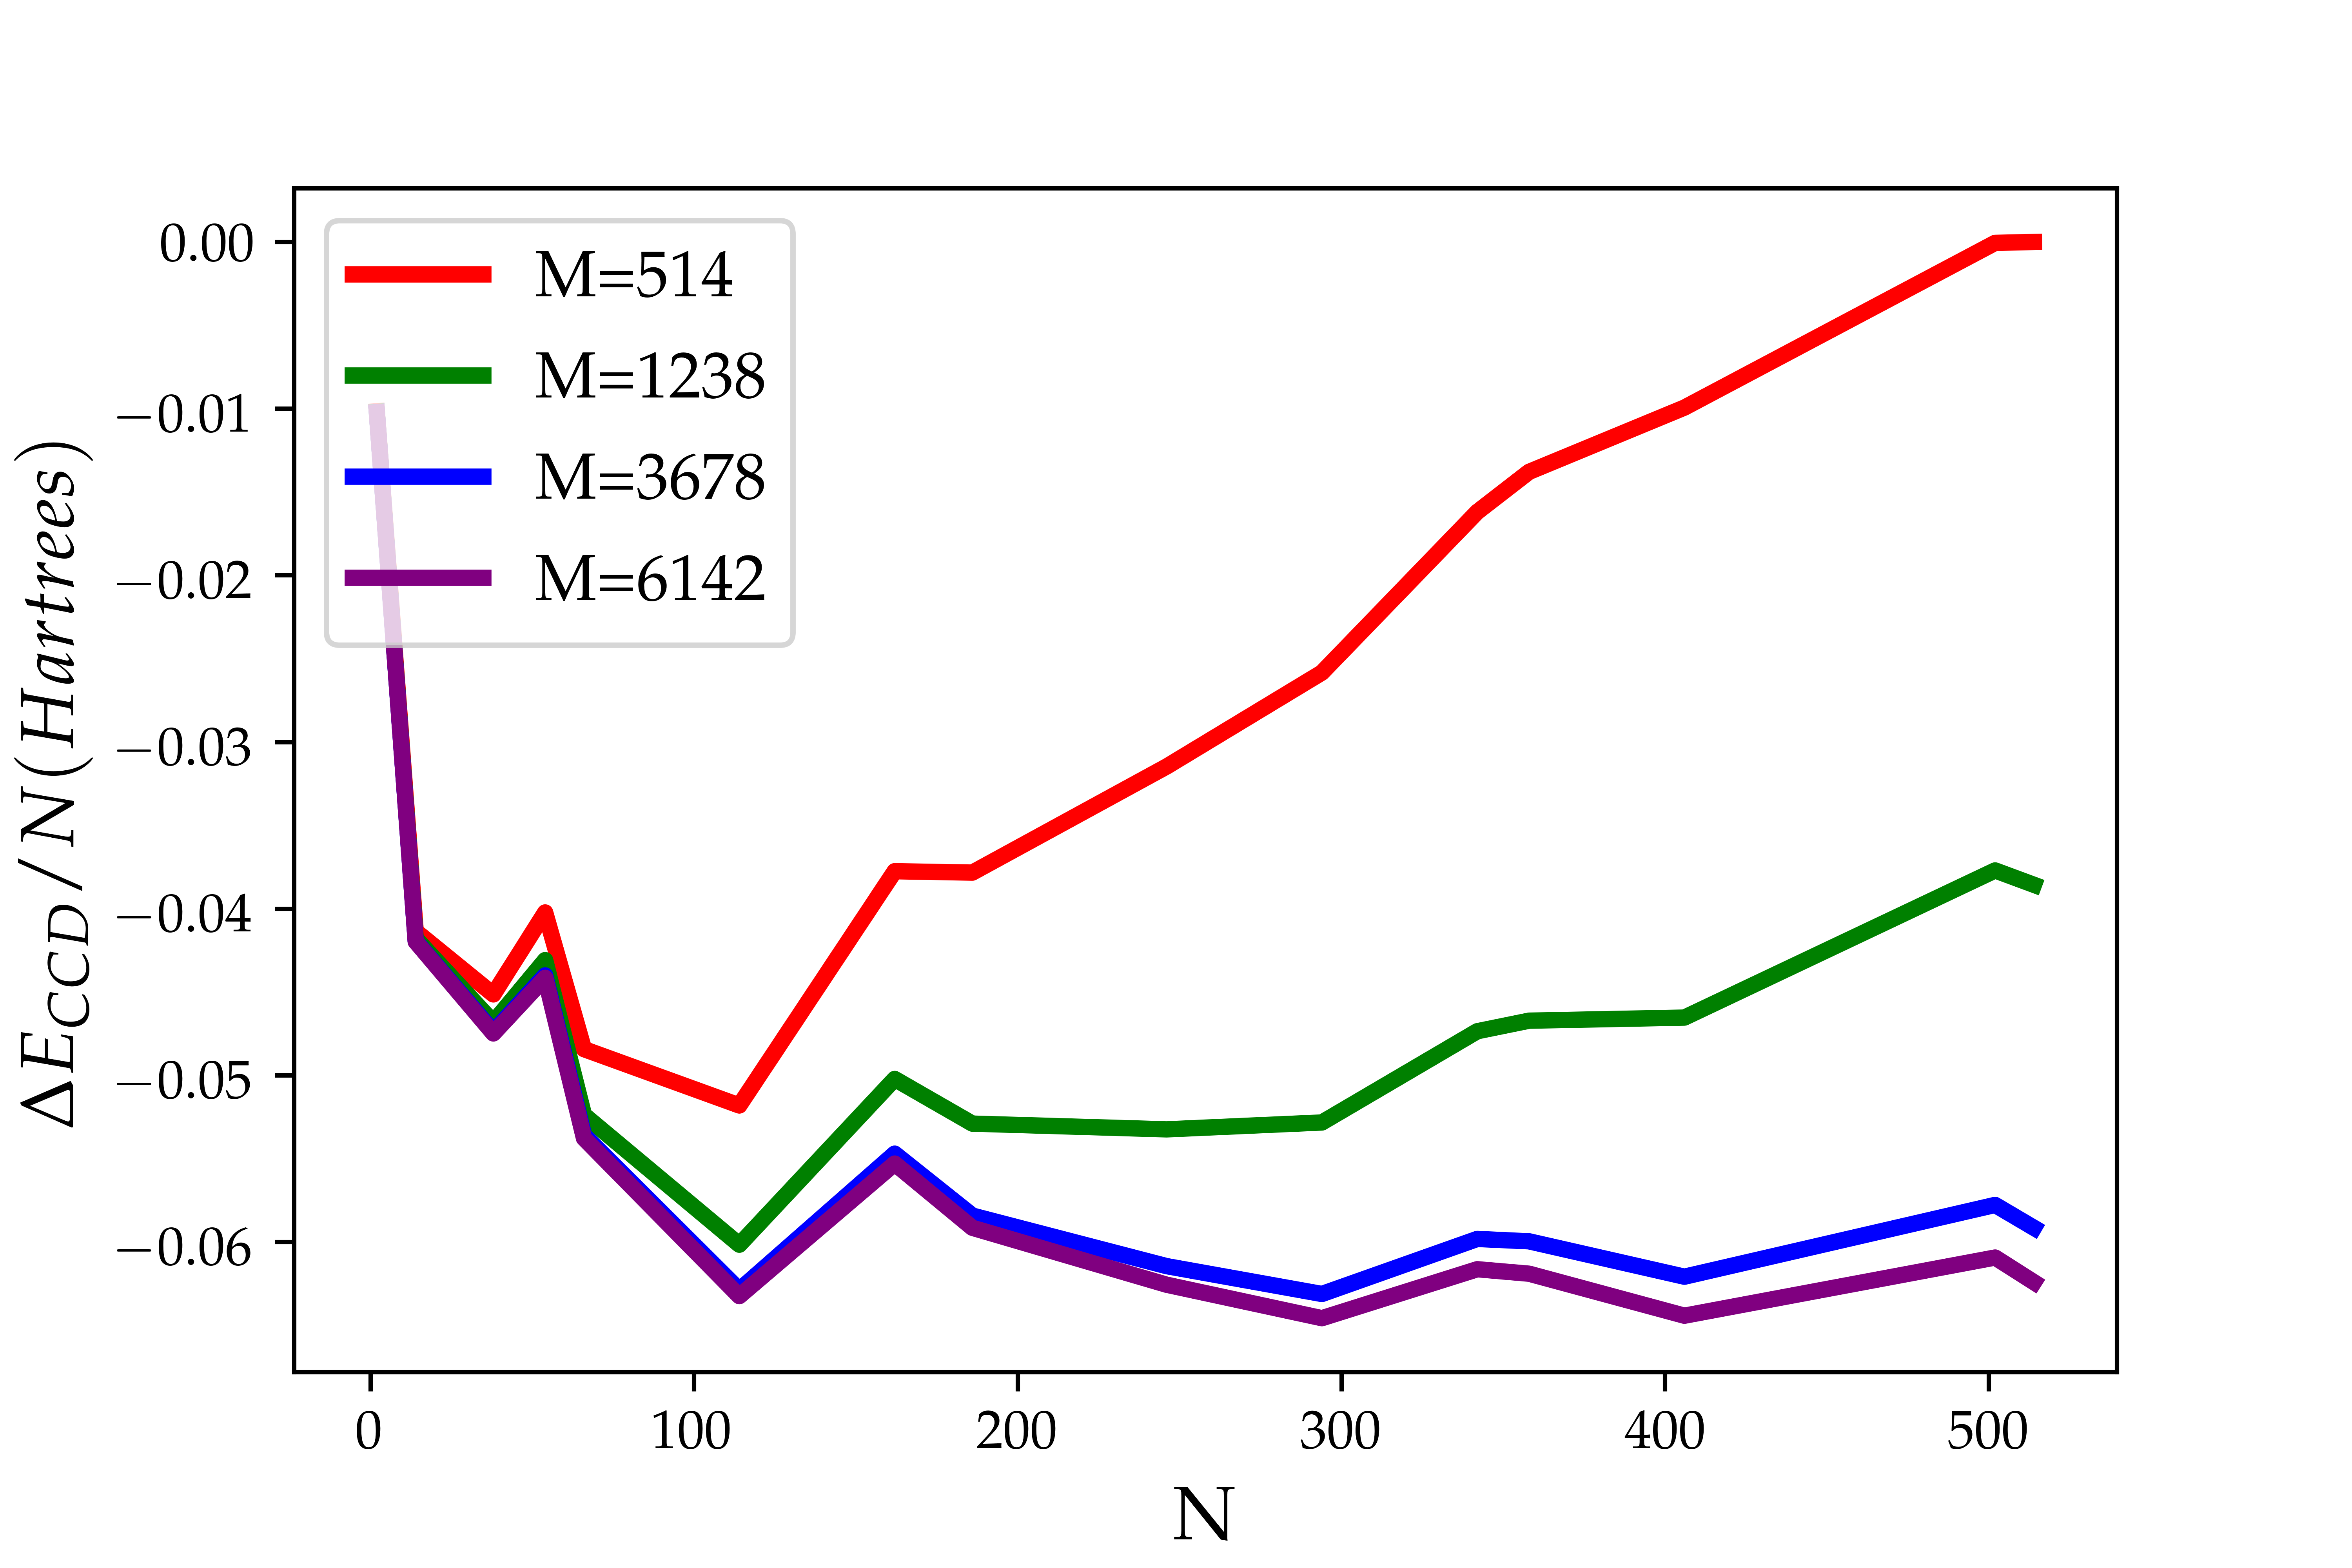
\includegraphics[scale=0.75]{Images/Chapter7/ElectronGas/Increase_M.png}
    \captionof{figure}{$\Delta E_{CC}$ per electron plotted against N with calculations performed at four different values of M. As M increases, the error in the calculation decreases, but the run time drastically increases.}
    \label{increase_m}
\end{figure}

Fig. \ref{fig:EG_times} shows the total run time in node seconds for CCD calculations of the HEG with $r_s$ = 0.5, N = 66, 294, or 514, and at various numbers of single-particle states. Node seconds will be used to report computational run times in this thesis such that run times generated with different numbers of MPI nodes can be compared. A \textit{node second} is defined as the run time of the coupled cluster program (in seconds) times the number of MPI nodes used in the calculation. For the HEG, all calculations were performed using nodes from Michigan State University's high-performance computing center. Each node is an Intel Xeon processor with a reported clock speed of 2.4 GHz. Each coupled cluster program was run with four MPI nodes and 28 OpenMP threads. The specifications of the coupled cluster code used to perform the HEG and neutron matter calculations with the Minnesota potential shown in the section are described in Ref. \cite{Ref5}.

In Fig. \ref{fig:EG_times}, there is a consistent pattern in the data where more electrons and more single-particle states in a calculation require a longer run time. This is an obvious and expected result, and in fact, the CCD run times should scale polynomially with the number of particles and single particle states allowed in the calculation. For example, a CCD calculation of the HEG should scale as $O(N^4M^6)$, where typically M >> N \cite{Ref2}. If we look at the results for N = 66 and assume that the converged CCD correlation energy occurs at M = 6,142 single-particle states (see Fig. \ref{increase_m}), the total run time for the CCD program is 653.88 node seconds (10.89 node minutes). However, generating the converged CCD correlation energy for N = 514 and M = 6,142 takes 42791.75 node seconds (11.88 \textbf{node hours}). Thus while generating the converged CCD correlation energies at a smaller number of particles results in possible computational run times, performing the same calculation at a large number of electrons is not feasible in most studies.

\begin{figure}
    \centering
    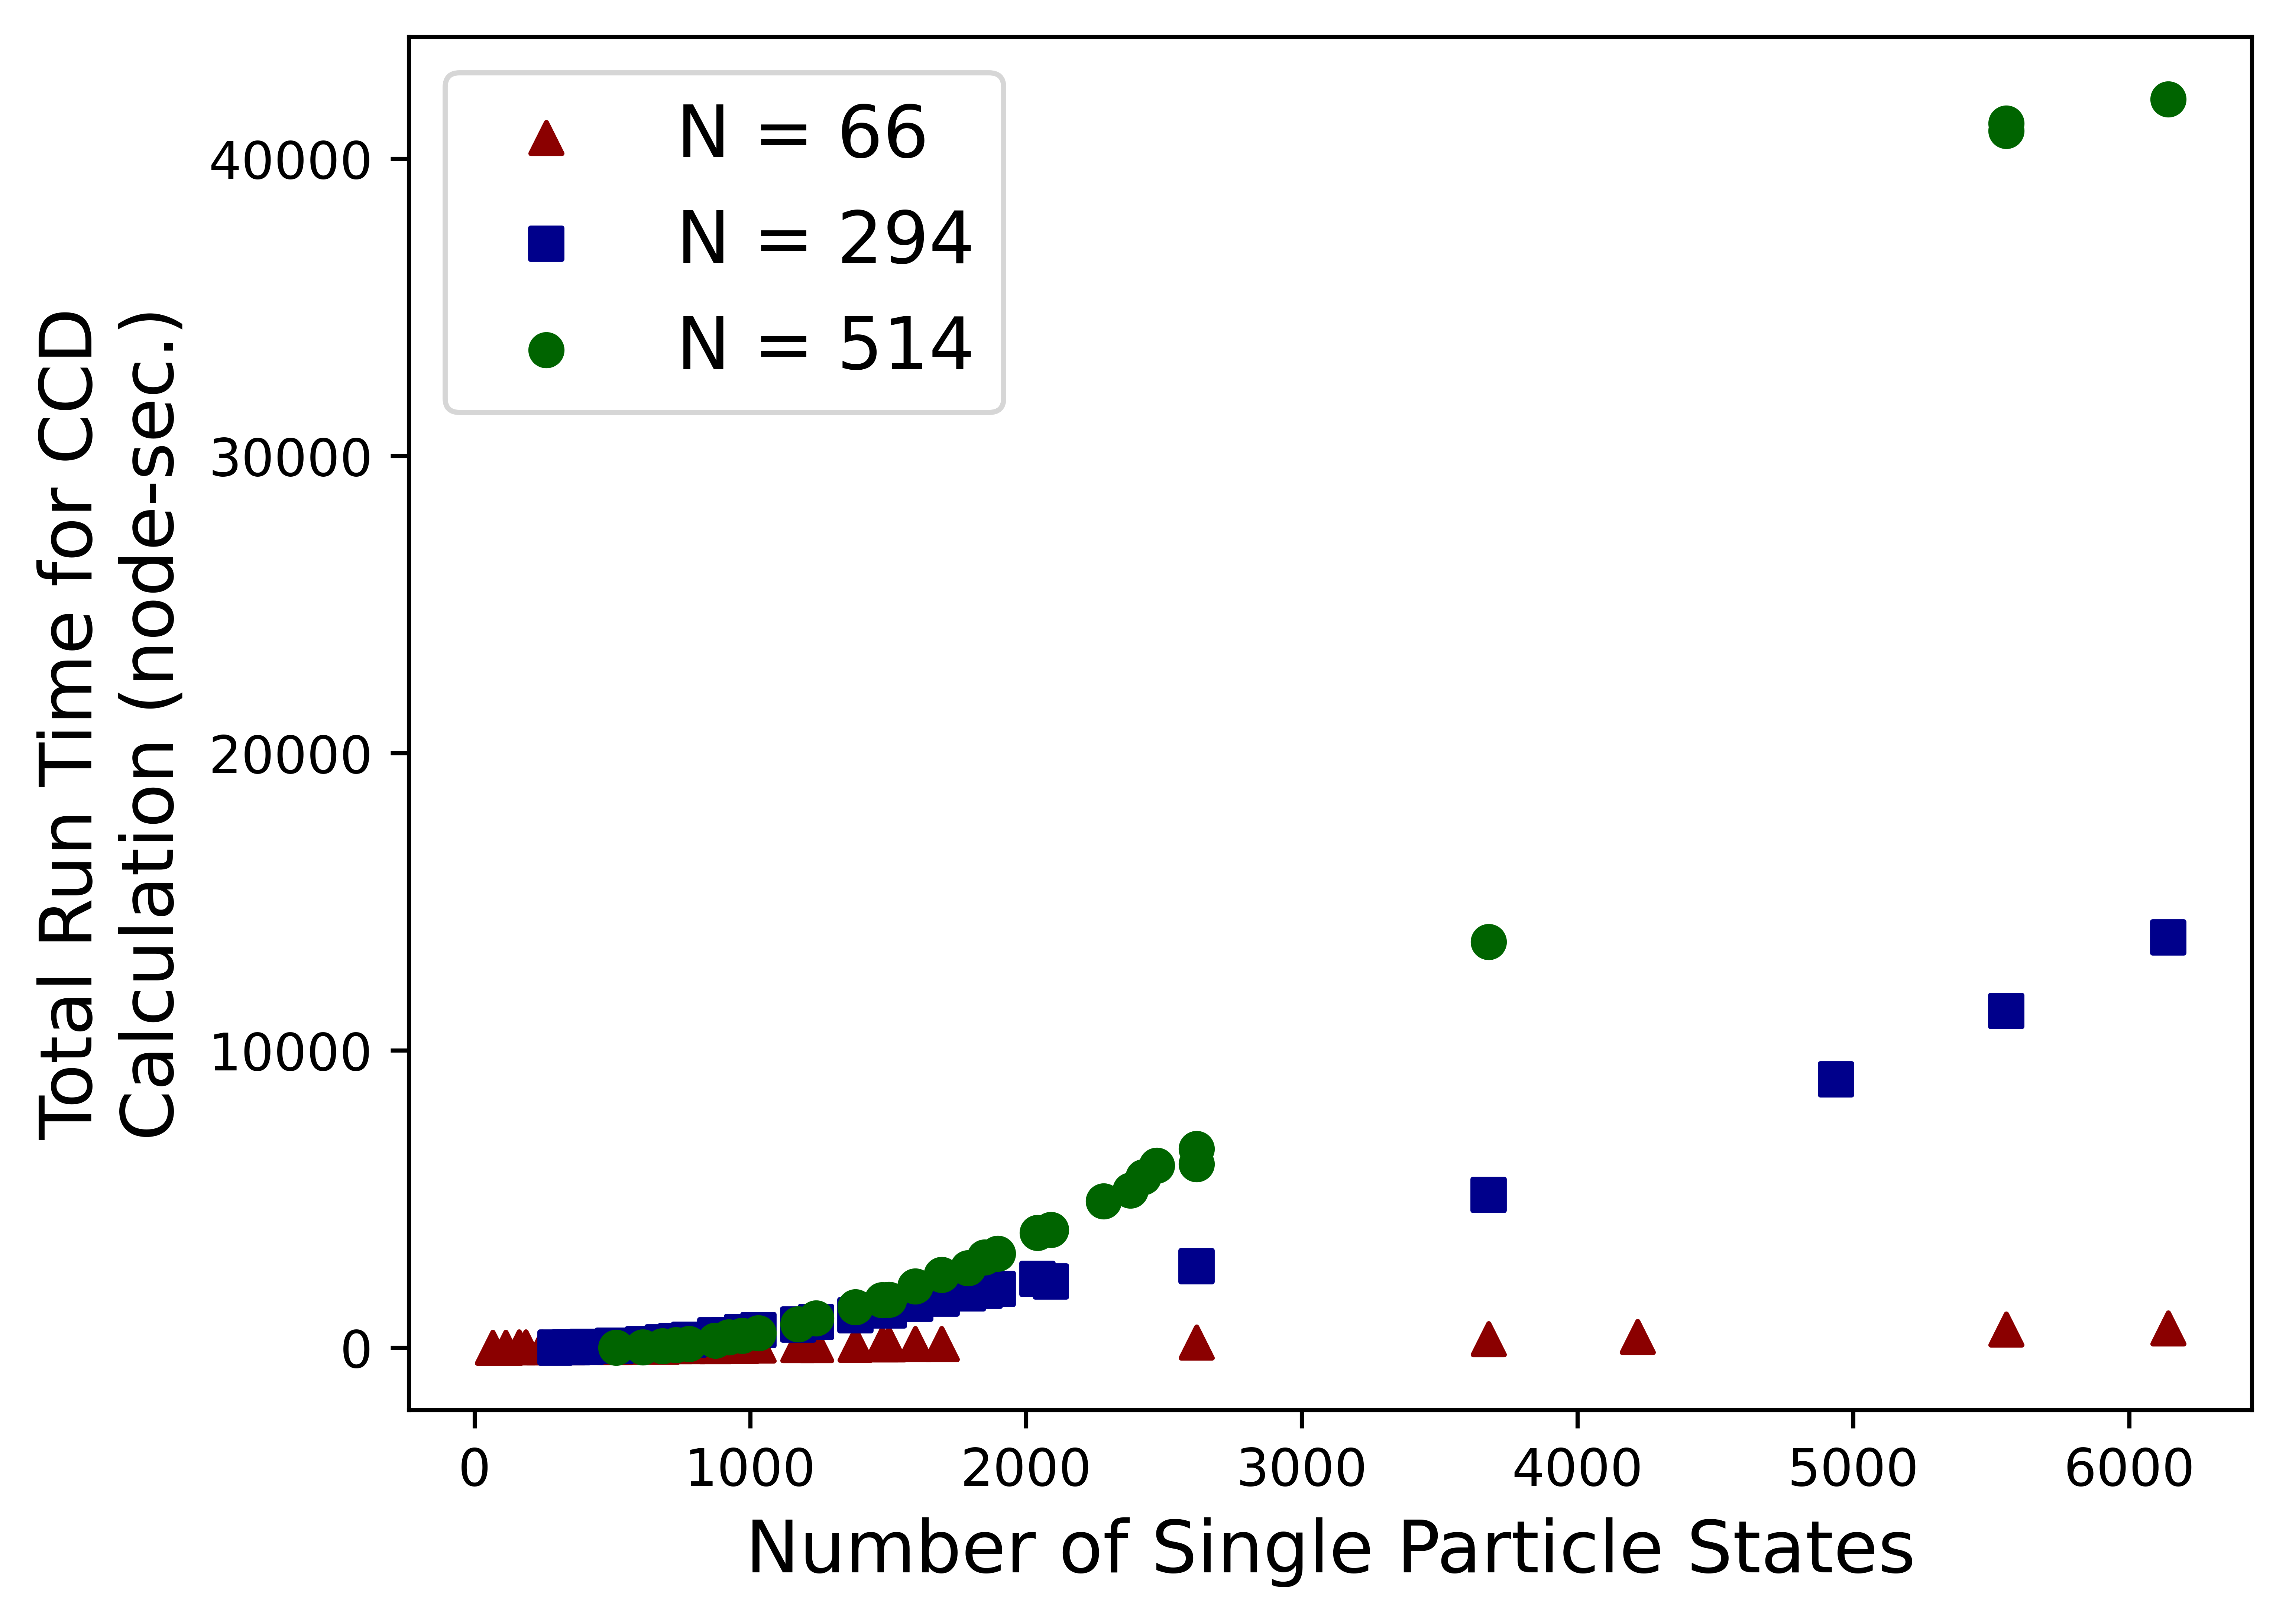
\includegraphics[scale=0.75]{Images/Chapter7/ElectronGas/EG_timing_graph_node_sec.png}
    \caption{The total run time needed, in node seconds, to perform a CCD calculation on the HEG with $r_s$ = 0.5 and at N = 66, 294, and 514. The CCD calculations are performed at many values of M, as shown on the x-axis. A node second is defined as the total run time of the program times the number of nodes used to run the program. Four nodes from Michigan State University's high-performance supercomputer were utilized in this case. These nodes have Intel Xeon processes with a clock speed of 2.4 GHz.}
    \label{fig:EG_times}
\end{figure}

Another factor we can look at is the amount of RAM needed to perform the CCD calculations at various numbers of electrons and single-particle states. The amount of RAM needed to perform the calculations should increase as both N and M increase as, naively, the Hamilton for the system should be ${MN}\choose{N}$ on each side. However, modern advancements limit the number of matrix elements that must be computed and stored. Fig. \ref{fig:eg_ram} shows the total amount of RAM (in gigabytes) needed to perform CCD calculations for the HEG at $r_s$ = 0.5. There are three different numbers of electrons represented in the figure: N = 66 (red triangles), N = 294 (blue squares), and N = 514 (green circles). These numbers of electrons span the range of interest for this work. The number of single-particle states varied from less than 1,000 to over 6,000. We see a consistent pattern in the data where the amount of RAM needed for the calculation increases as the number of electrons and single-particle states changes. The converged CCD correlation energy for 514 electrons (the highest amount of electrons in this thesis) and at 6,142 single particle states takes a startling 283.79 GB of RAM to run. However, the converged CCD correlation energy at 66 electrons and 6,142 single particle states still takes 106.49 GB of RAM, a very moderate number of particles to have in a calculation. Therefore, not only is computing the converged CCD correlation energies expensive in the amount of computational time required, but the converged correlation energies also take a considerable amount of computational resources, requiring a supercomputer for these calculations to be feasible.

\begin{figure}
    \centering
    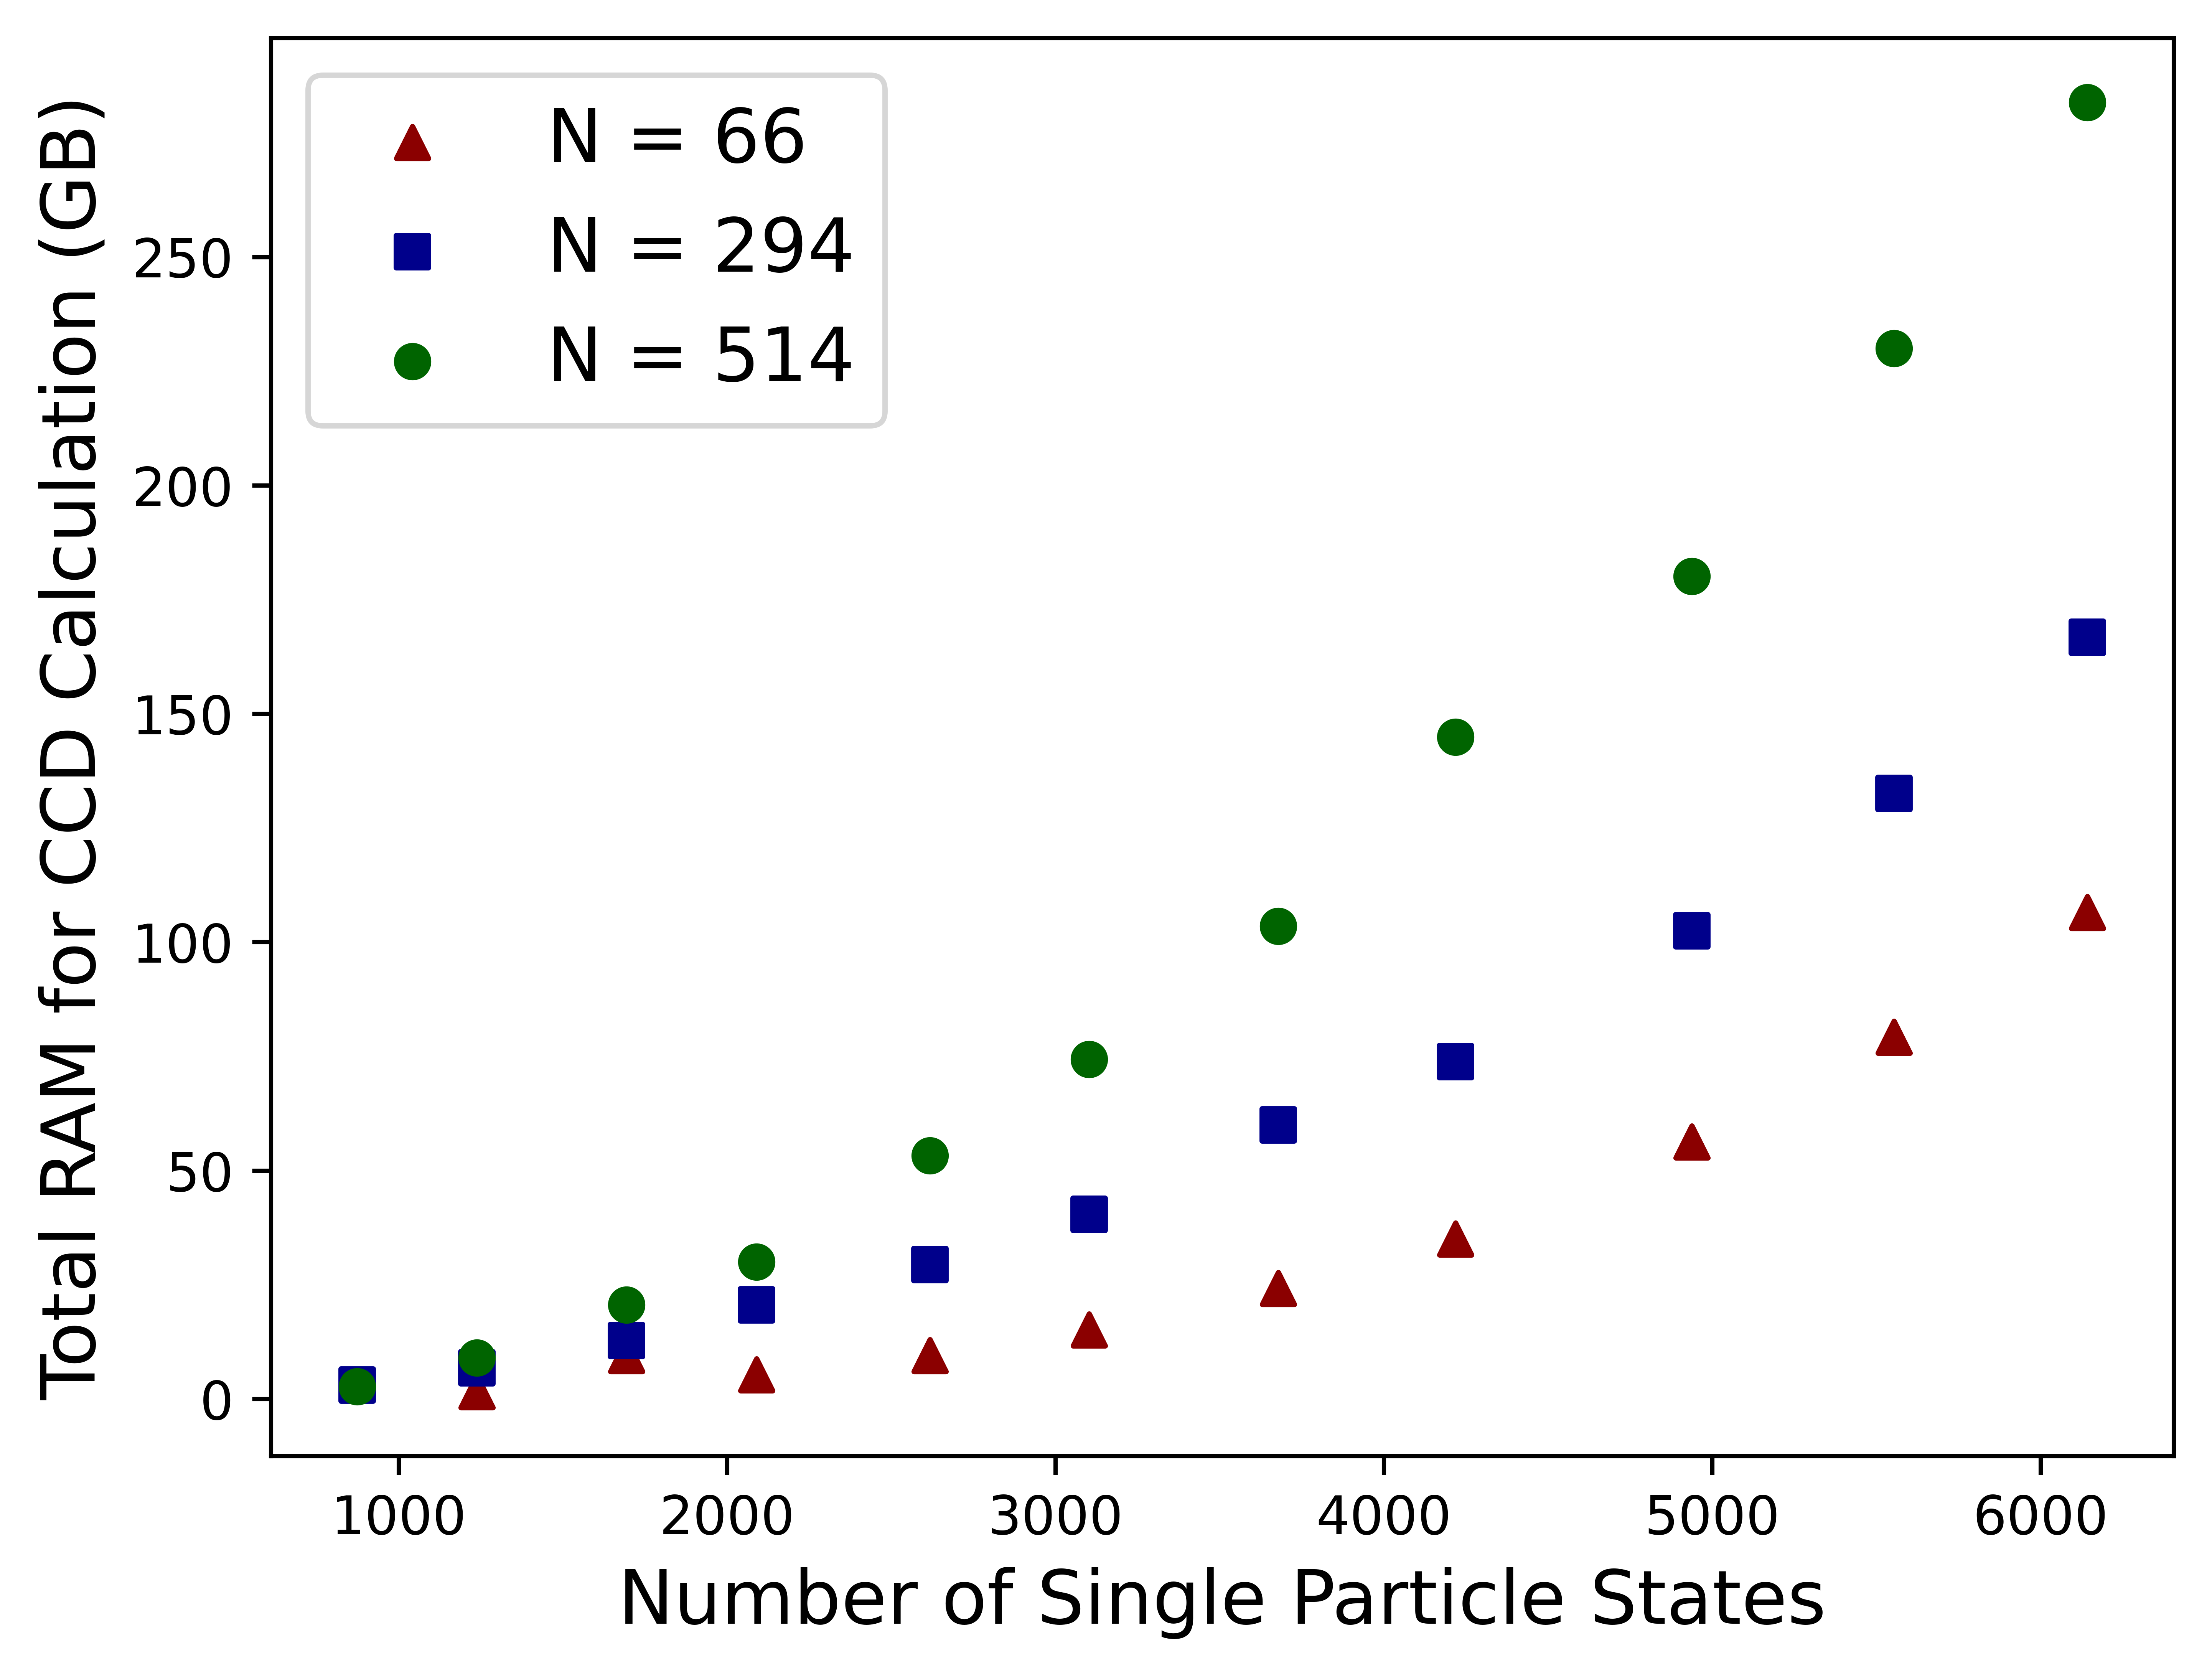
\includegraphics[scale=0.75]{Images/Chapter7/EG_RAM.png}
    \caption{The total amount of RAM in gigabytes needed to perform CCD calculations on the HEG with $r_s$ = 0.5 and with 66, 294, or 514 electrons.  Calculations were performed at various numbers of single-particle states (x-axis).}
    \label{fig:eg_ram}
\end{figure}

%% COMPLETE THE MOTIVATION HERE 
Thus, though increasing the number of single-particle states in a CCD calculation of the HEG increases the accuracy of the CCD correlation energy, it comes with high computational time and resource considerations that can make these calculations infeasible. Therefore, we are motivated to develop a method by which the CCD correlation energies at a high number of single-particle states can be recreated using only calculations performed at a lower number of single-particle states, where the computational resource and time requirements are significantly more reasonable.

In Fig. \ref{mbpt_and_cc}, $\Delta E_{CCD}$ and $\Delta E_{MBPT2}$ is plotted as a function of the number of single-particle states in the calculation for a HEG system with $r_s$ = 0.5 and 342 electrons. The CCD results are plotted in red, and the MBPT results are in blue. The calculations up to 2,090 single-particle states are plotted with the solid lines, and then the converged correlation energies are plotted with the dashed lines. It is much easier in this figure to see that the correlation energies converge as the number of single-particle states increases and that even at around 2,000 single-particle states, the correlation energies are not close to their converged values. However, the ranges of single-particle states shown in this figure with the solid lines are the calculations we wish to use to predict the converged CCD correlation energy, as at these ranges, the computational time and resource requirements are reasonable.

There are a few important things to note in Fig. \ref{mbpt_and_cc}.  First, there is a significant difference between the converged correlation energies, meaning that even though it is easier to generate $\Delta E_{MBPT}$ compared to $\Delta E_{CC}$, $\Delta E_{MBPT}$ is not a good approximation to the true correlation energy. Second, though it takes 21,735.10 node seconds (6.03 node hours) to calculate $\Delta E_{CC,6142}^{342}$ it only takes 5.12 node seconds to generate $\Delta E_{MBPT,6142}^{342}$.  Thus generating the converged MBPT2 correlation energies is significantly faster than generating the converged CCD correlation energies. The MBPT2 calculations are faster by four orders of magnitude. Finally, note that though the MBPT2 and CCD calculations converge to different values, they converge at roughly the same rate and display similar patterns in their convergence. This similarity in convergence was the inspiration for the SRE method.

\begin{figure}
    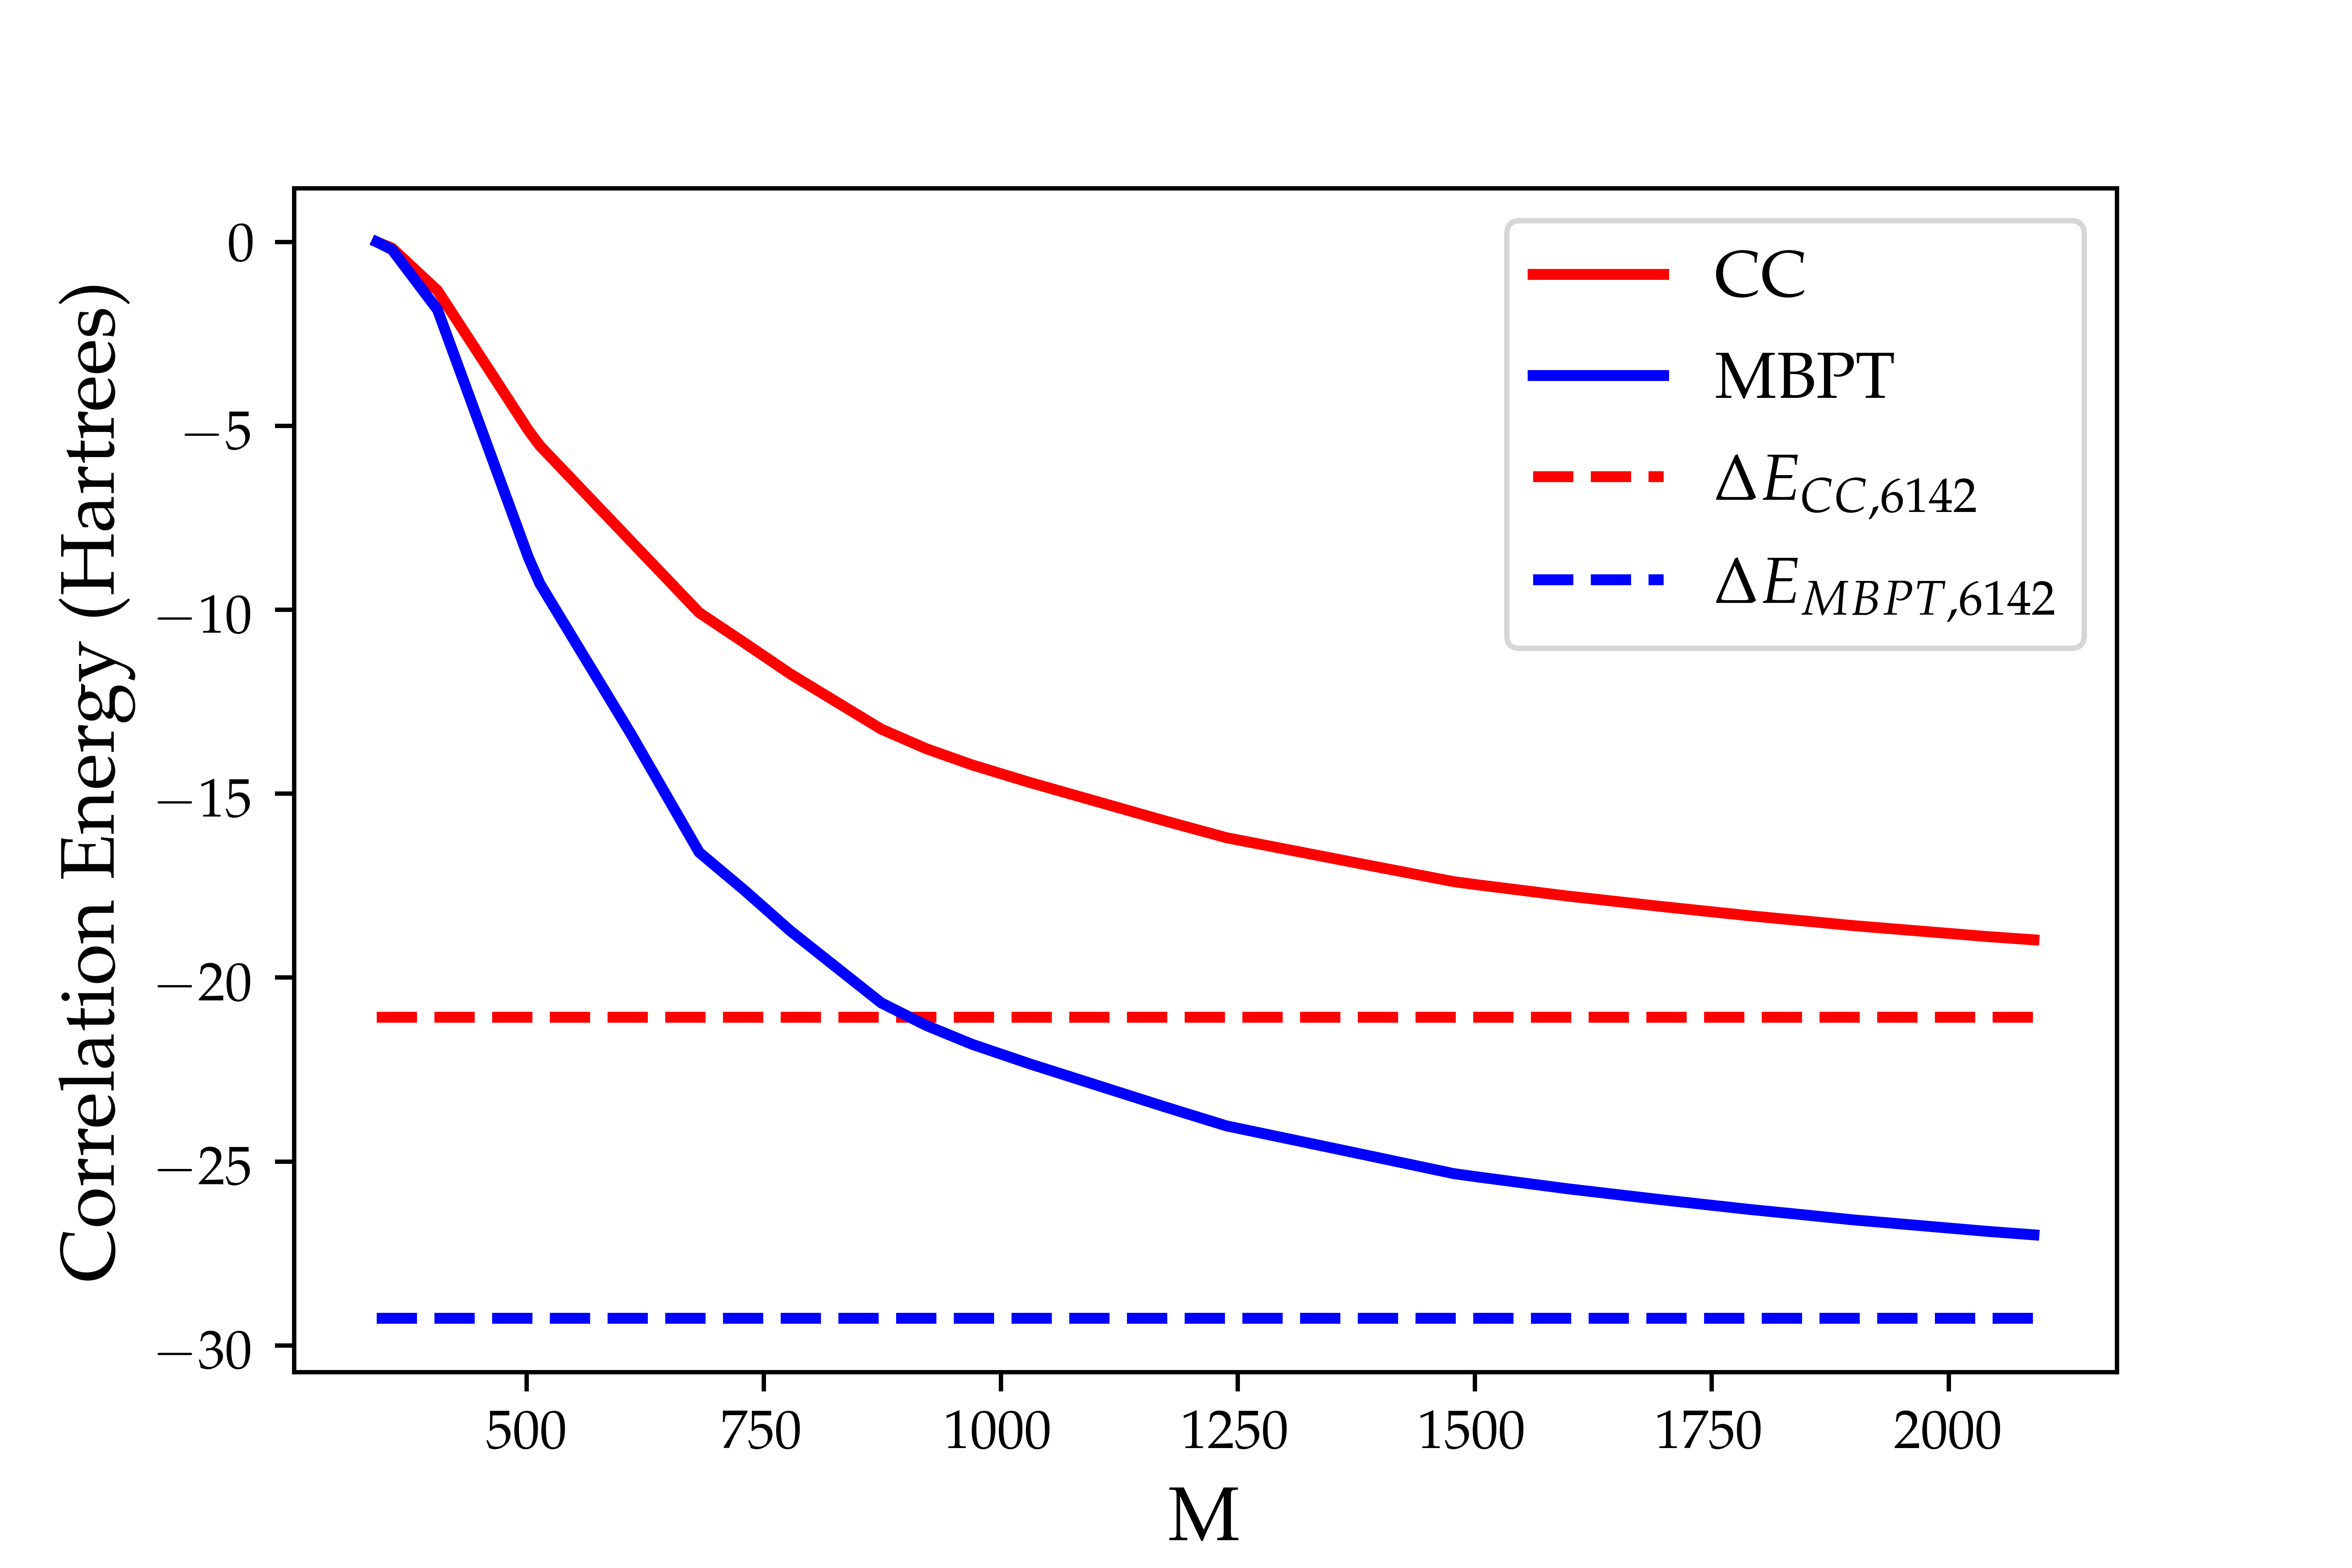
\includegraphics[scale=0.75]{Images/Chapter7/ElectronGas/MBPT_and_CC.png}
    \captionof{figure}{A plot of $\Delta E_{CC}$ and $\Delta E_{MBPT}$ versus M for a HEG system with N=342 and r$_s$=0.5.  The converged correlation energies calculated at M=6142 are shown with dashed lines.}
    \label{mbpt_and_cc}
\end{figure}

Next, we will take Fig. \ref{mbpt_and_cc} and reformat it such that $\Delta E_{CC}$ is plotted as a function of $\Delta E_{MBPT}$ (Fig. \ref{mbpt_vs_cc}).  Each point is at a constant value of M in this format, and M increases from the right to the left. In Fig. \ref{mbpt_vs_cc}, note that the graph is relatively linear, and in fact, it becomes more linear from right to left. Put another way, the graph of $\Delta E_{CC}$ versus $\Delta E_{MBPT}$ becomes more linear as M increases because as M increases, both correlation energies converge. We can check this using Fig. \ref{slopes}

\begin{figure}
    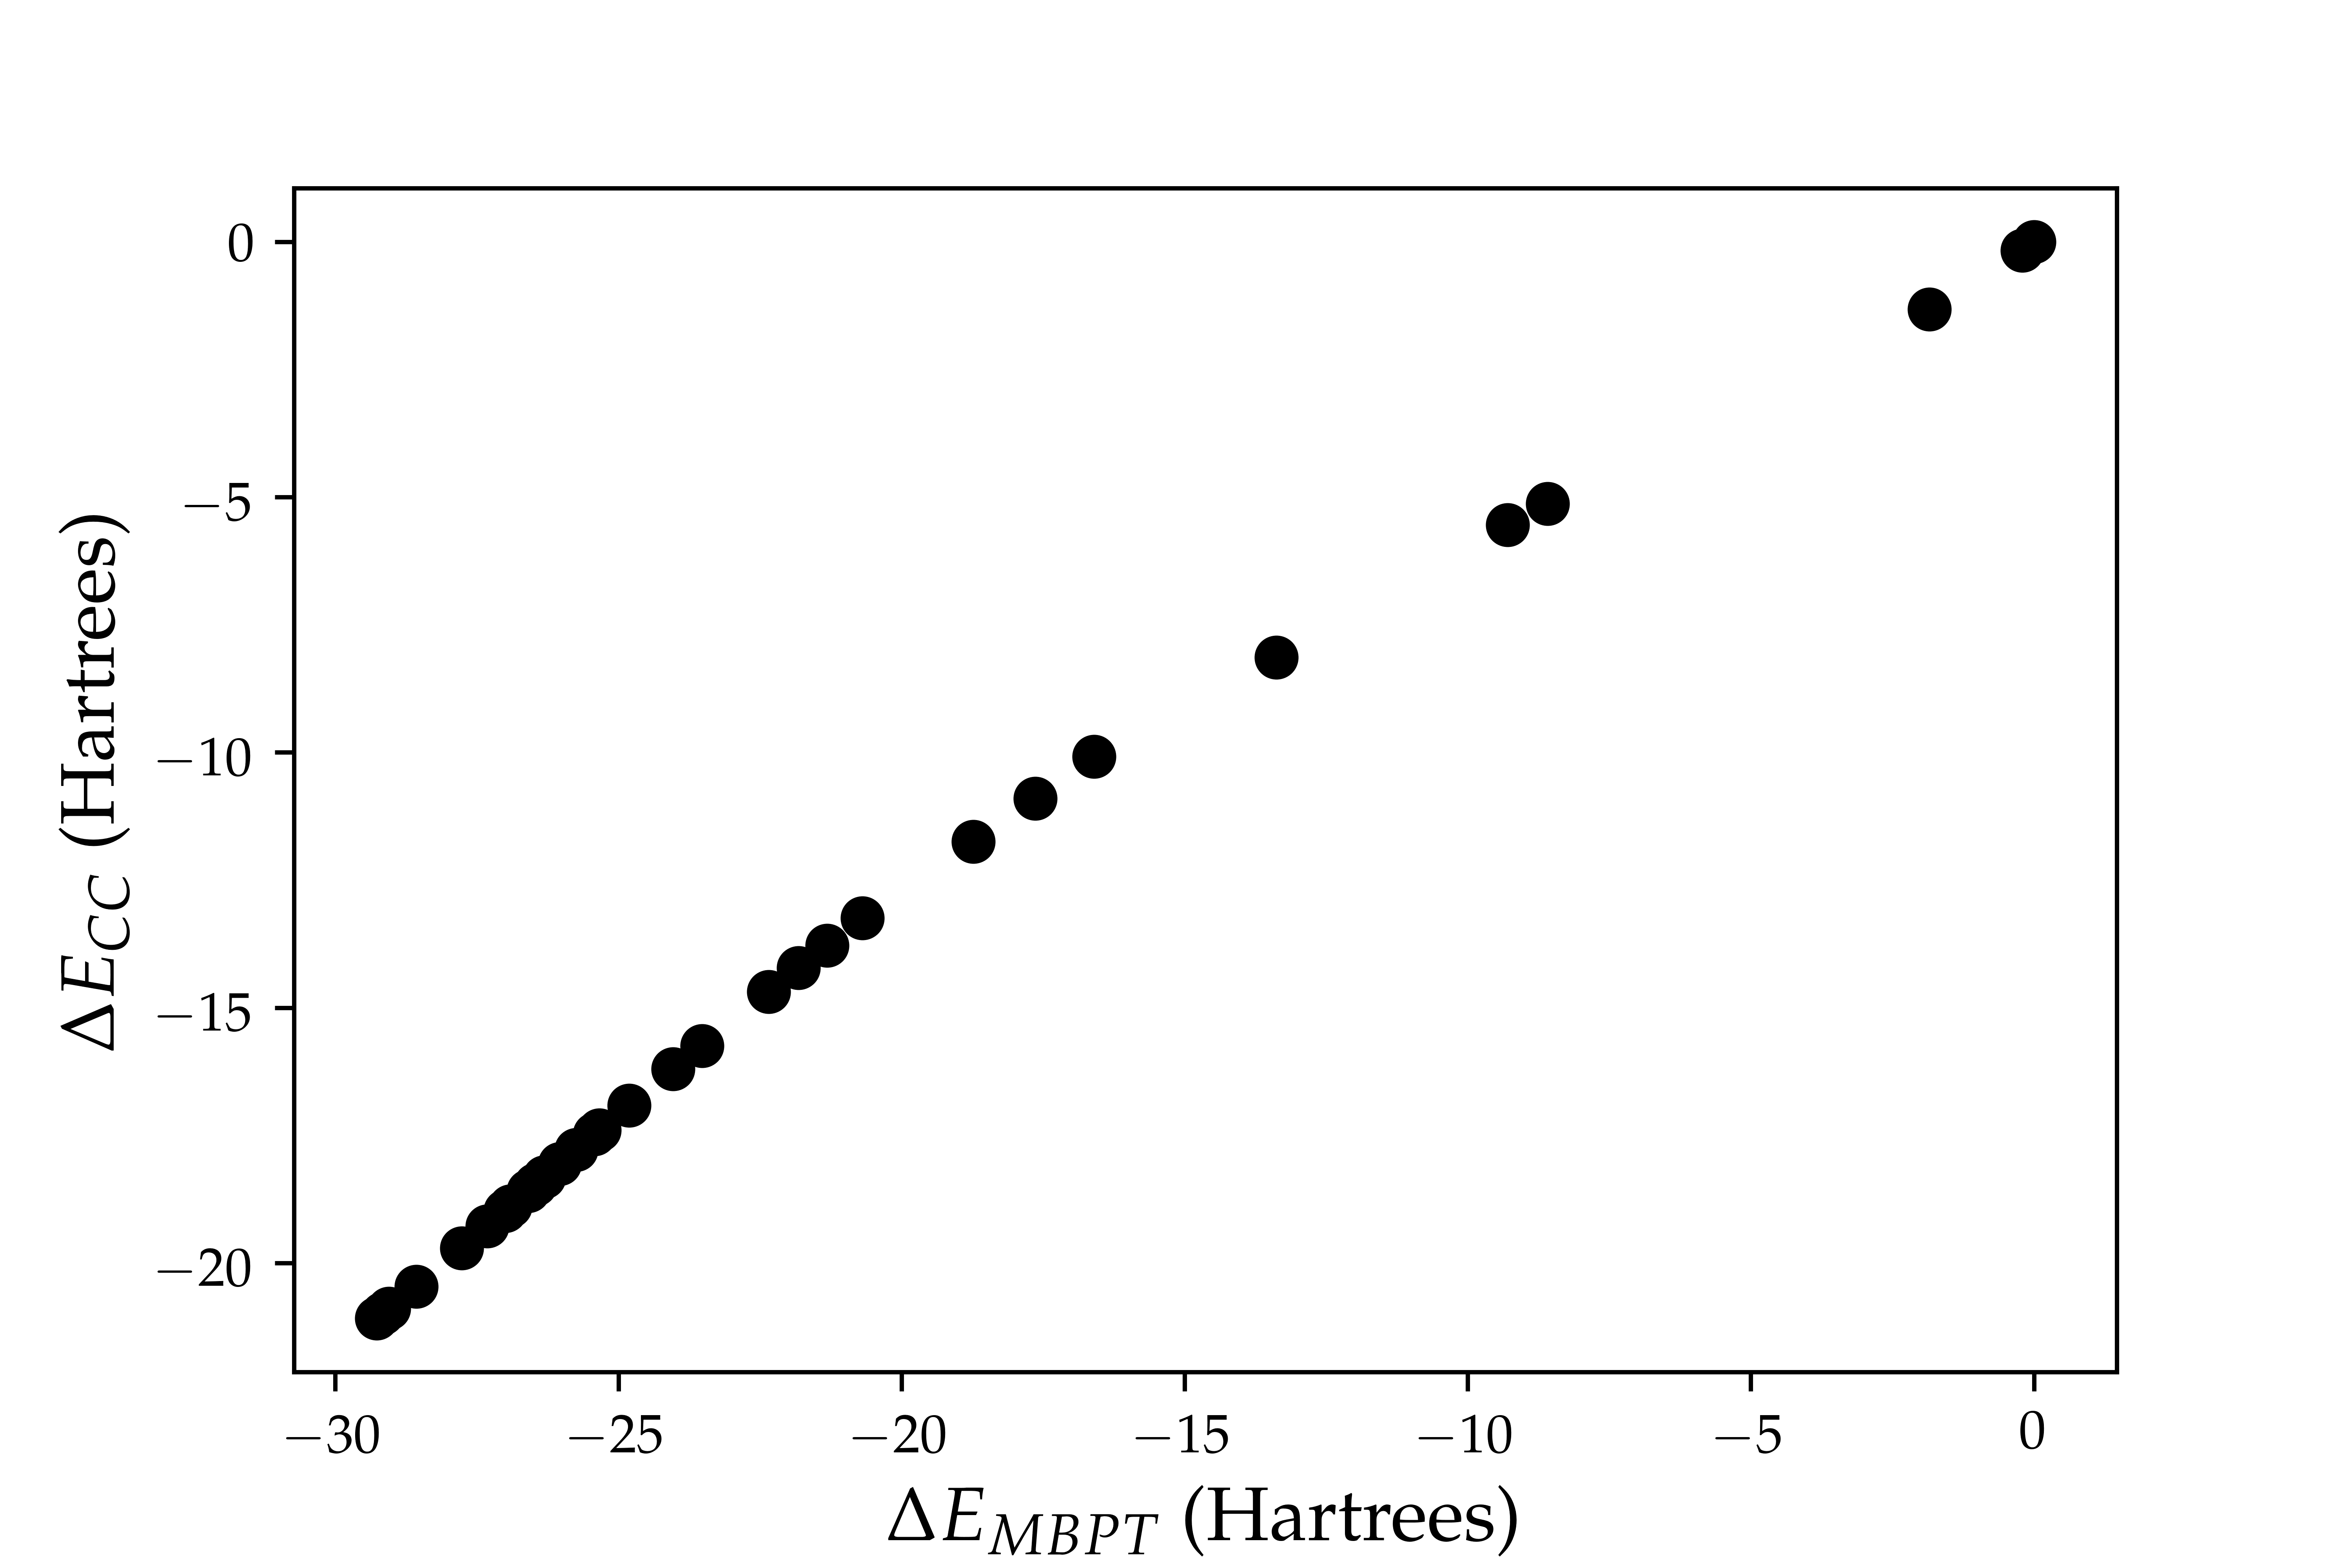
\includegraphics[scale=0.75]{Images/Chapter7/ElectronGas/MBPT_vs_CC.png}
    \captionof{figure}{Figure \ref{mbpt_and_cc} is transformed such that $\Delta E_{CC}$ are plotted as a function of t$\Delta E_{MBPT}$ (such that each point has the same M). The resulting plot has a linear relationship that becomes stronger to the left (as M increases).}
    \label{mbpt_vs_cc}
\end{figure}

Fig. \ref{slopes} shows the ratio of $\Delta E_{CC}$/$\Delta E_{MBPT}$ as a function of the number of single-particle states in the calculations for three different numbers of electrons for calculations of the HEG at $r_s$ = 0.5. The ratio $\Delta E_{CC}$/$\Delta E_{MBPT}$ is the slope of the line in Fig. \ref{mbpt_vs_cc}. While the slopes are rapidly changing at lower values of M, by the end of the graph, all of the slopes are constant, though the slopes at higher numbers of electrons converge slower than the slopes at lower numbers of electrons. However, this graph does verify that the slopes will become constant, and the SRE method should work if we can accurately predict this slope.

\begin{center}
    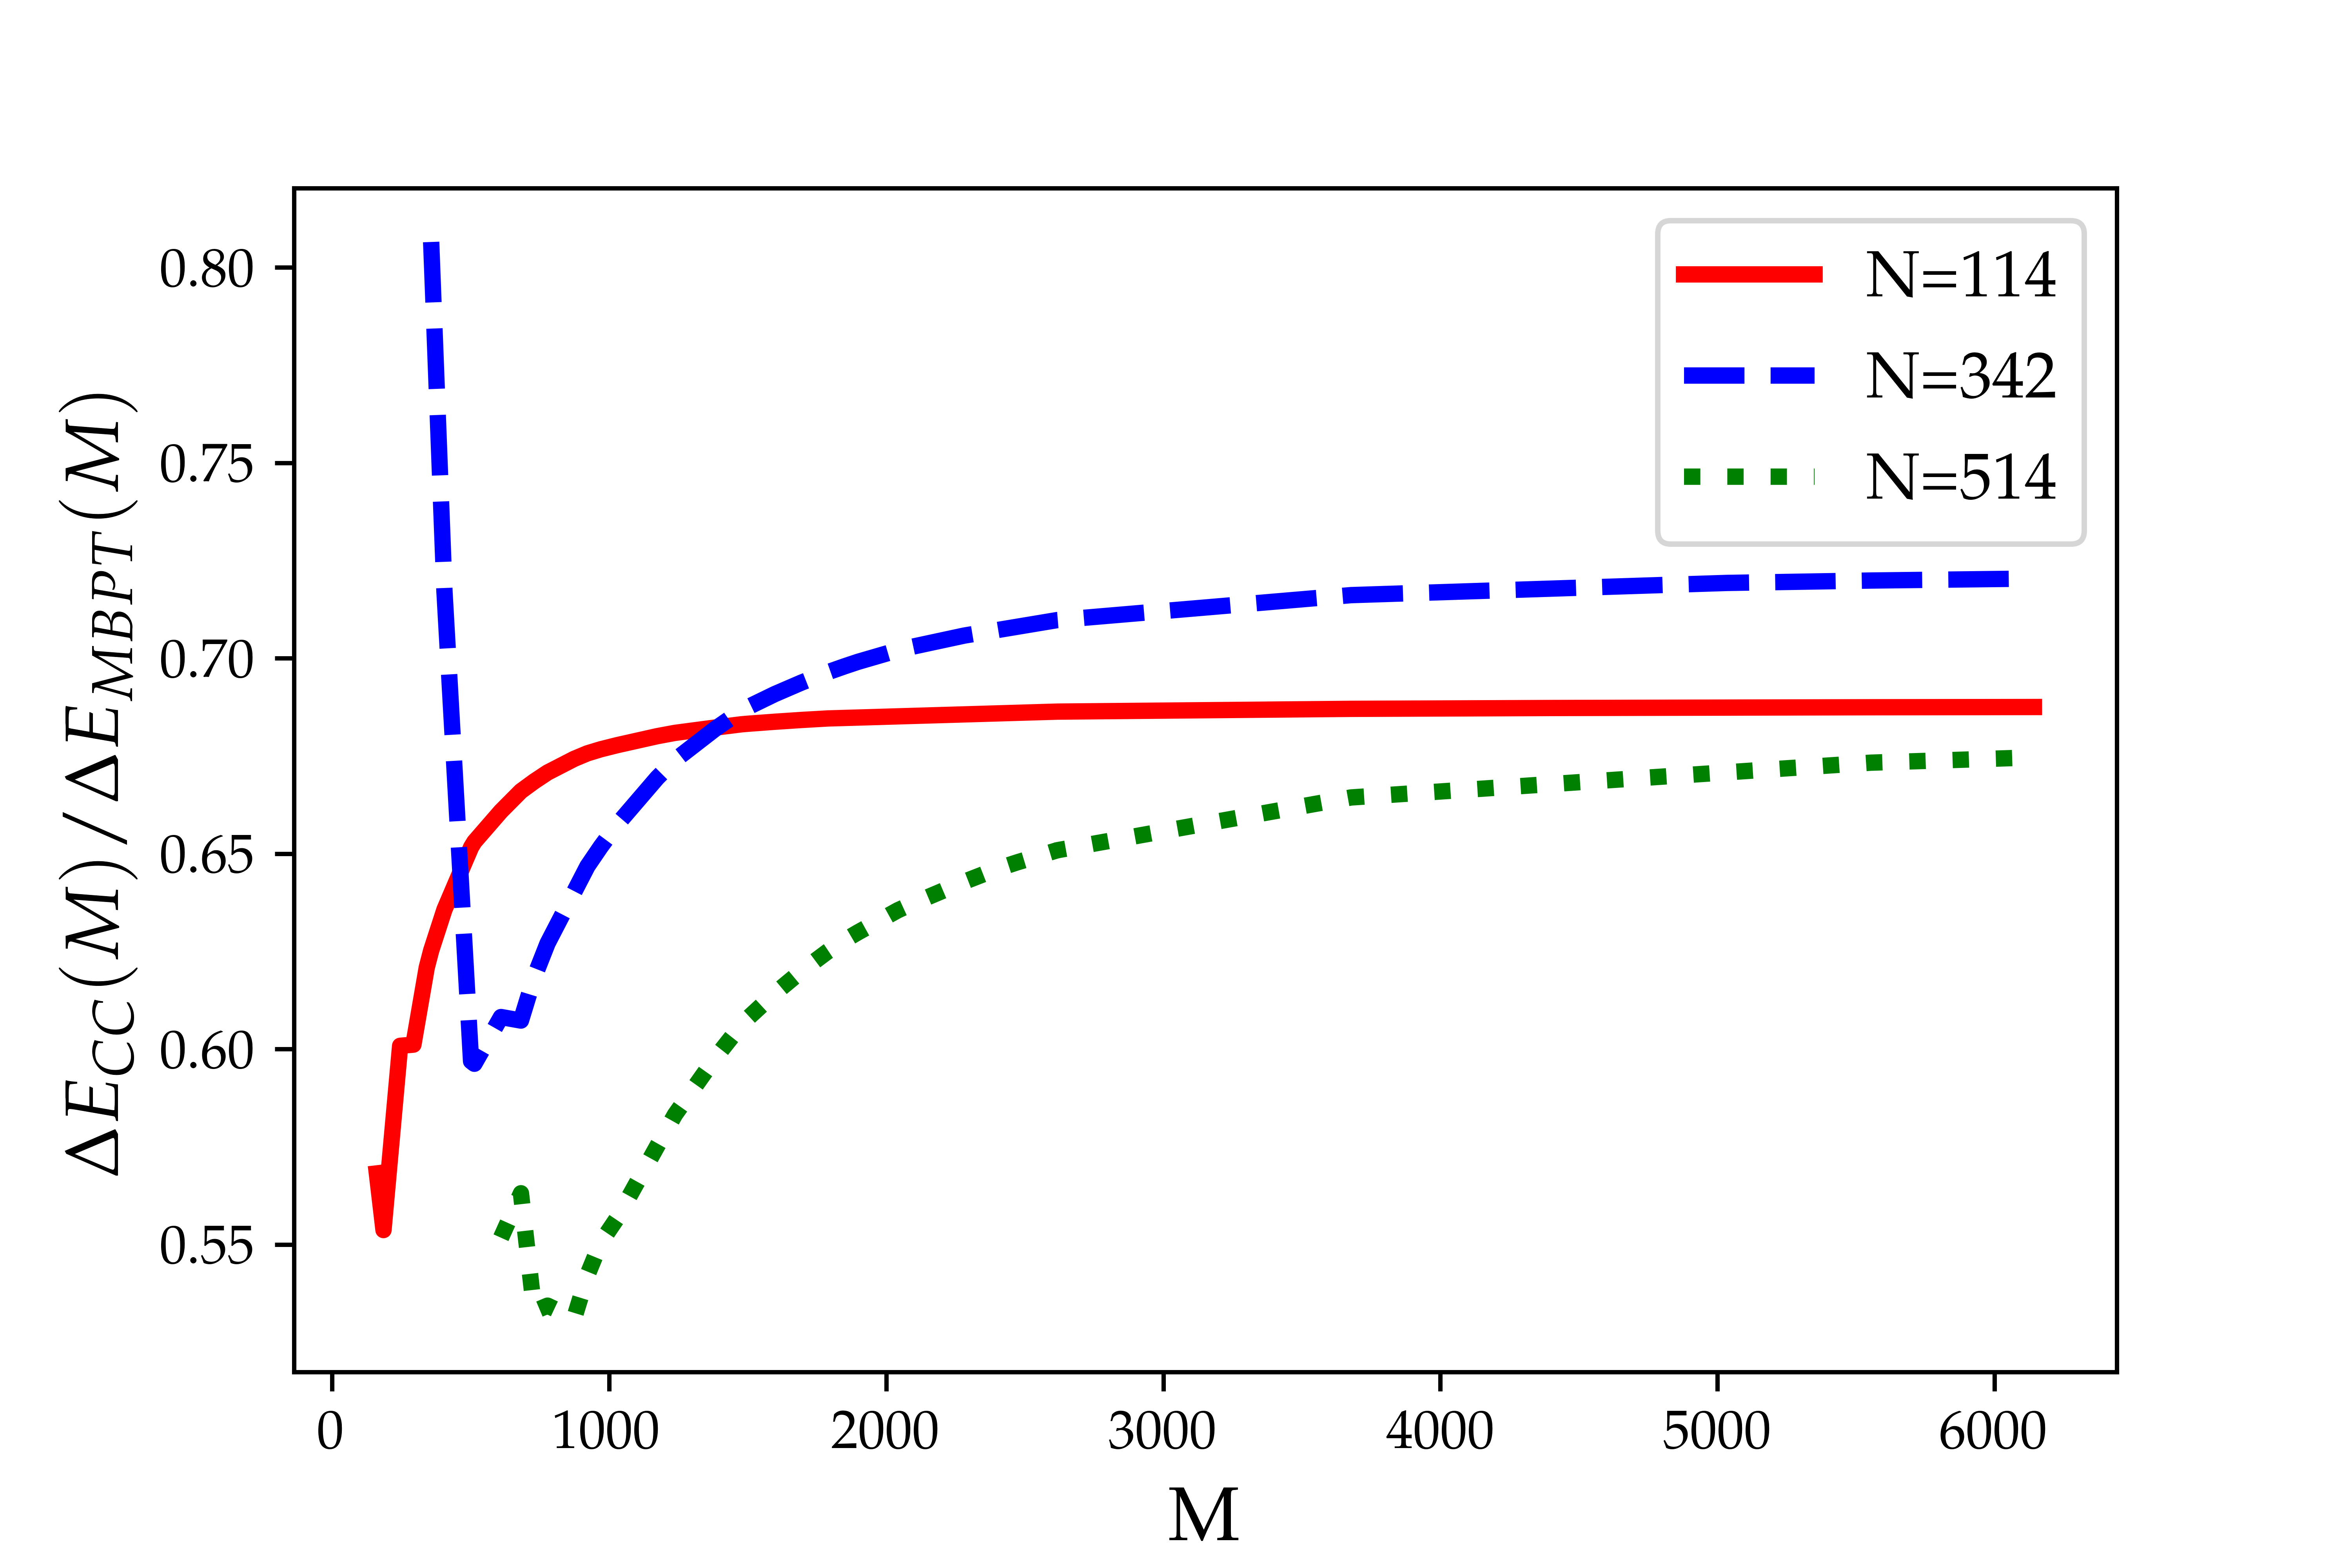
\includegraphics[scale=0.75]{Images/Chapter7/ElectronGas/Slopes.png}
    \captionof{figure}{A plot of the ratio of $\Delta E_{CC}$ to $\Delta E_{MBPT}$ as a function of M for N=114, 342, and 514 and r$_s$=0.5.  As M increases, the ratio (or the slope of the line in Figure FIGURE NUMBER) becomes increasingly constant. However, it is important to note that the run time increases drastically as M increases.}
    \label{slopes}
\end{center}
    \subsection*{Traditional Extrapolation Methods}
Before we begin to develop in full the SRE method for determining the converged CCD correlation energies with respect to the number of single-particle states in the calculation, let us look at two traditional methods for removing the basis incompleteness error and two methods that may work based on the analysis from the last section.

%% TRUNCATE
The most common way to deal with a basis incompleteness error is to truncate the number of single-particle states at some high number. Fig. \ref{fig:compare_no_sre} displays the results of truncating the calculations at 20 open shells, corresponding to between 922 and 2,090 single particle states depending on the number of electrons in the calculation for a HEG with $r_s$ = 0.5. This graph, plotted in orange, is compared to the correlation energy calculation performed at 70 total energy shells (M = 6,142) in black, which are the fully converged results where the basis incompleteness error is eliminated. Of course, one way to negate the basis incompleteness error is to perform calculations at very high numbers of single-particle states. However, as we saw in the last section, this is not necessarily feasible due to the high computational time and resource requirements, and, therefore, simply increasing the number of single-particle states in the system is not an attractive option for removing the basis incompleteness error.

%% POWER LAW
Another common method is to find the correlation energy in the complete basis limit by using a power law of the form:

\begin{equation}
    \Delta E_{CCD}(M) = E_{CCD,\infty} + AM^{-\alpha},
\end{equation}

where $E_{CCD,\infty}$ (the correlation energy in the complete basis limit) and A are fit to data from correlation energy calculations at several different values of M. The value of $\alpha$ is typically fixed to 1, so this method is generally referred to as a 1/M power law (REFERENCE HERE). The results of performing this power law fit on a HEG system with $r_s$ = 0.5 and using 16 data points per number of electrons (from 5 open shells to 20 open shells) are shown in Fig. \ref{fig:compare_no_sre} in blue.  We can see that this power law fit overestimates the HEG correlation energies by about the same margin that the truncation at 20 open shells underestimated them. This indicates that for the data available, neither of these traditional methods of removing the basis incompleteness error are attractive option. The power law does not provide a good fit and overestimates the correlation energies; while truncating the basis at a large number of single-particle states can provide an accurate result, the computational time and resource requirements make this option not feasible for many systems.

%% SLOPE at SET SHELL NUMBER
Next, we can look at two methods inspired by the analysis performed in the previous section. In Fig. \ref{mbpt_vs_cc}, the graph is reasonably linear if we plot the CCD correlation energies as a function of the MBPT2 correlation energies. The first approach to calculating the converged CCD correlation energies from this plot may be to take the CCD and MBPT2 calculation at a relatively high number of single-particle states, create the ratio $m = \Delta E_{CCD}/\Delta E_{MBPT2}$, and then take m and multiply it by the MBPT2 correlation energy at a very high number of single-particle states to approximate the CCD correlation energy at that same high number of single-particle states (here M = 6,142): $\Delta E_{CCD, 6142} \approx m\Delta E_{MBPT2, 6142}$. For this investigation, we derived the slope from calculations performed at 20 open energy shells (the same truncation level we used earlier), then calculated the slope and generated a prediction for the CCD correlation energy at 6,142 single-particle states. This analysis's results are shown in green in Fig. \ref{fig:compare_pnm_all_no_sre}. We can see that this is a much better approximation of the converged CCD correlation energies than the previous two attempts. However, there are still significant deviations at higher numbers of electrons. Therefore, while this is an improvement, we will seek a better method to accurately predict the converged correlation energies at all numbers of electrons, including the high values.

%% LINEAR REGRESSION
As a final method, we will use linear regression to fit a subset of the data shown in Fig. \ref{mbpt_vs_cc}.  It should be noted that even though machine learning is quite a simple machine learning algorithm, this is our first machine learning approach to remove the basis incompleteness error from these calculations.

For training the linear regression algorithm, we will use 16 sets of MBPT2 and CCD correlation energies drawn from calculations between 5 and 20 open shells (the exact number of single-particle states depends on the number of electrons). First, the linear regression algorithm will be trained and then asked to predict $\Delta E_{CCD, 6142}$ by giving $\Delta E_{MBPT2,6142}$. It is important to remember that generating MBPT2 correlation energies is a fast computation.

The results of performing this analysis are shown in red in Fig. \ref{fig:compare_no_sre}. These results are similar to the previous slope analysis, where the correlation energies at lower numbers of electrons are well matched, but there are deviations at higher numbers. We could improve this result by using training data drawn from higher M values. However, like the other methods shown here, that is an unattractive solution due to the increased computational time and resource requirements.

%% ERROR COMPARISON AND CONCLUSION

Thus the two traditional extrapolation methods we have looked at and the two new methods fail to satisfactorily remove the basis incompleteness errors without requiring data drawn from calculations with a much higher number of single-particle states. Thus, we need to be in a position to begin fully developing the SRE method.

\begin{figure}
    \centering
    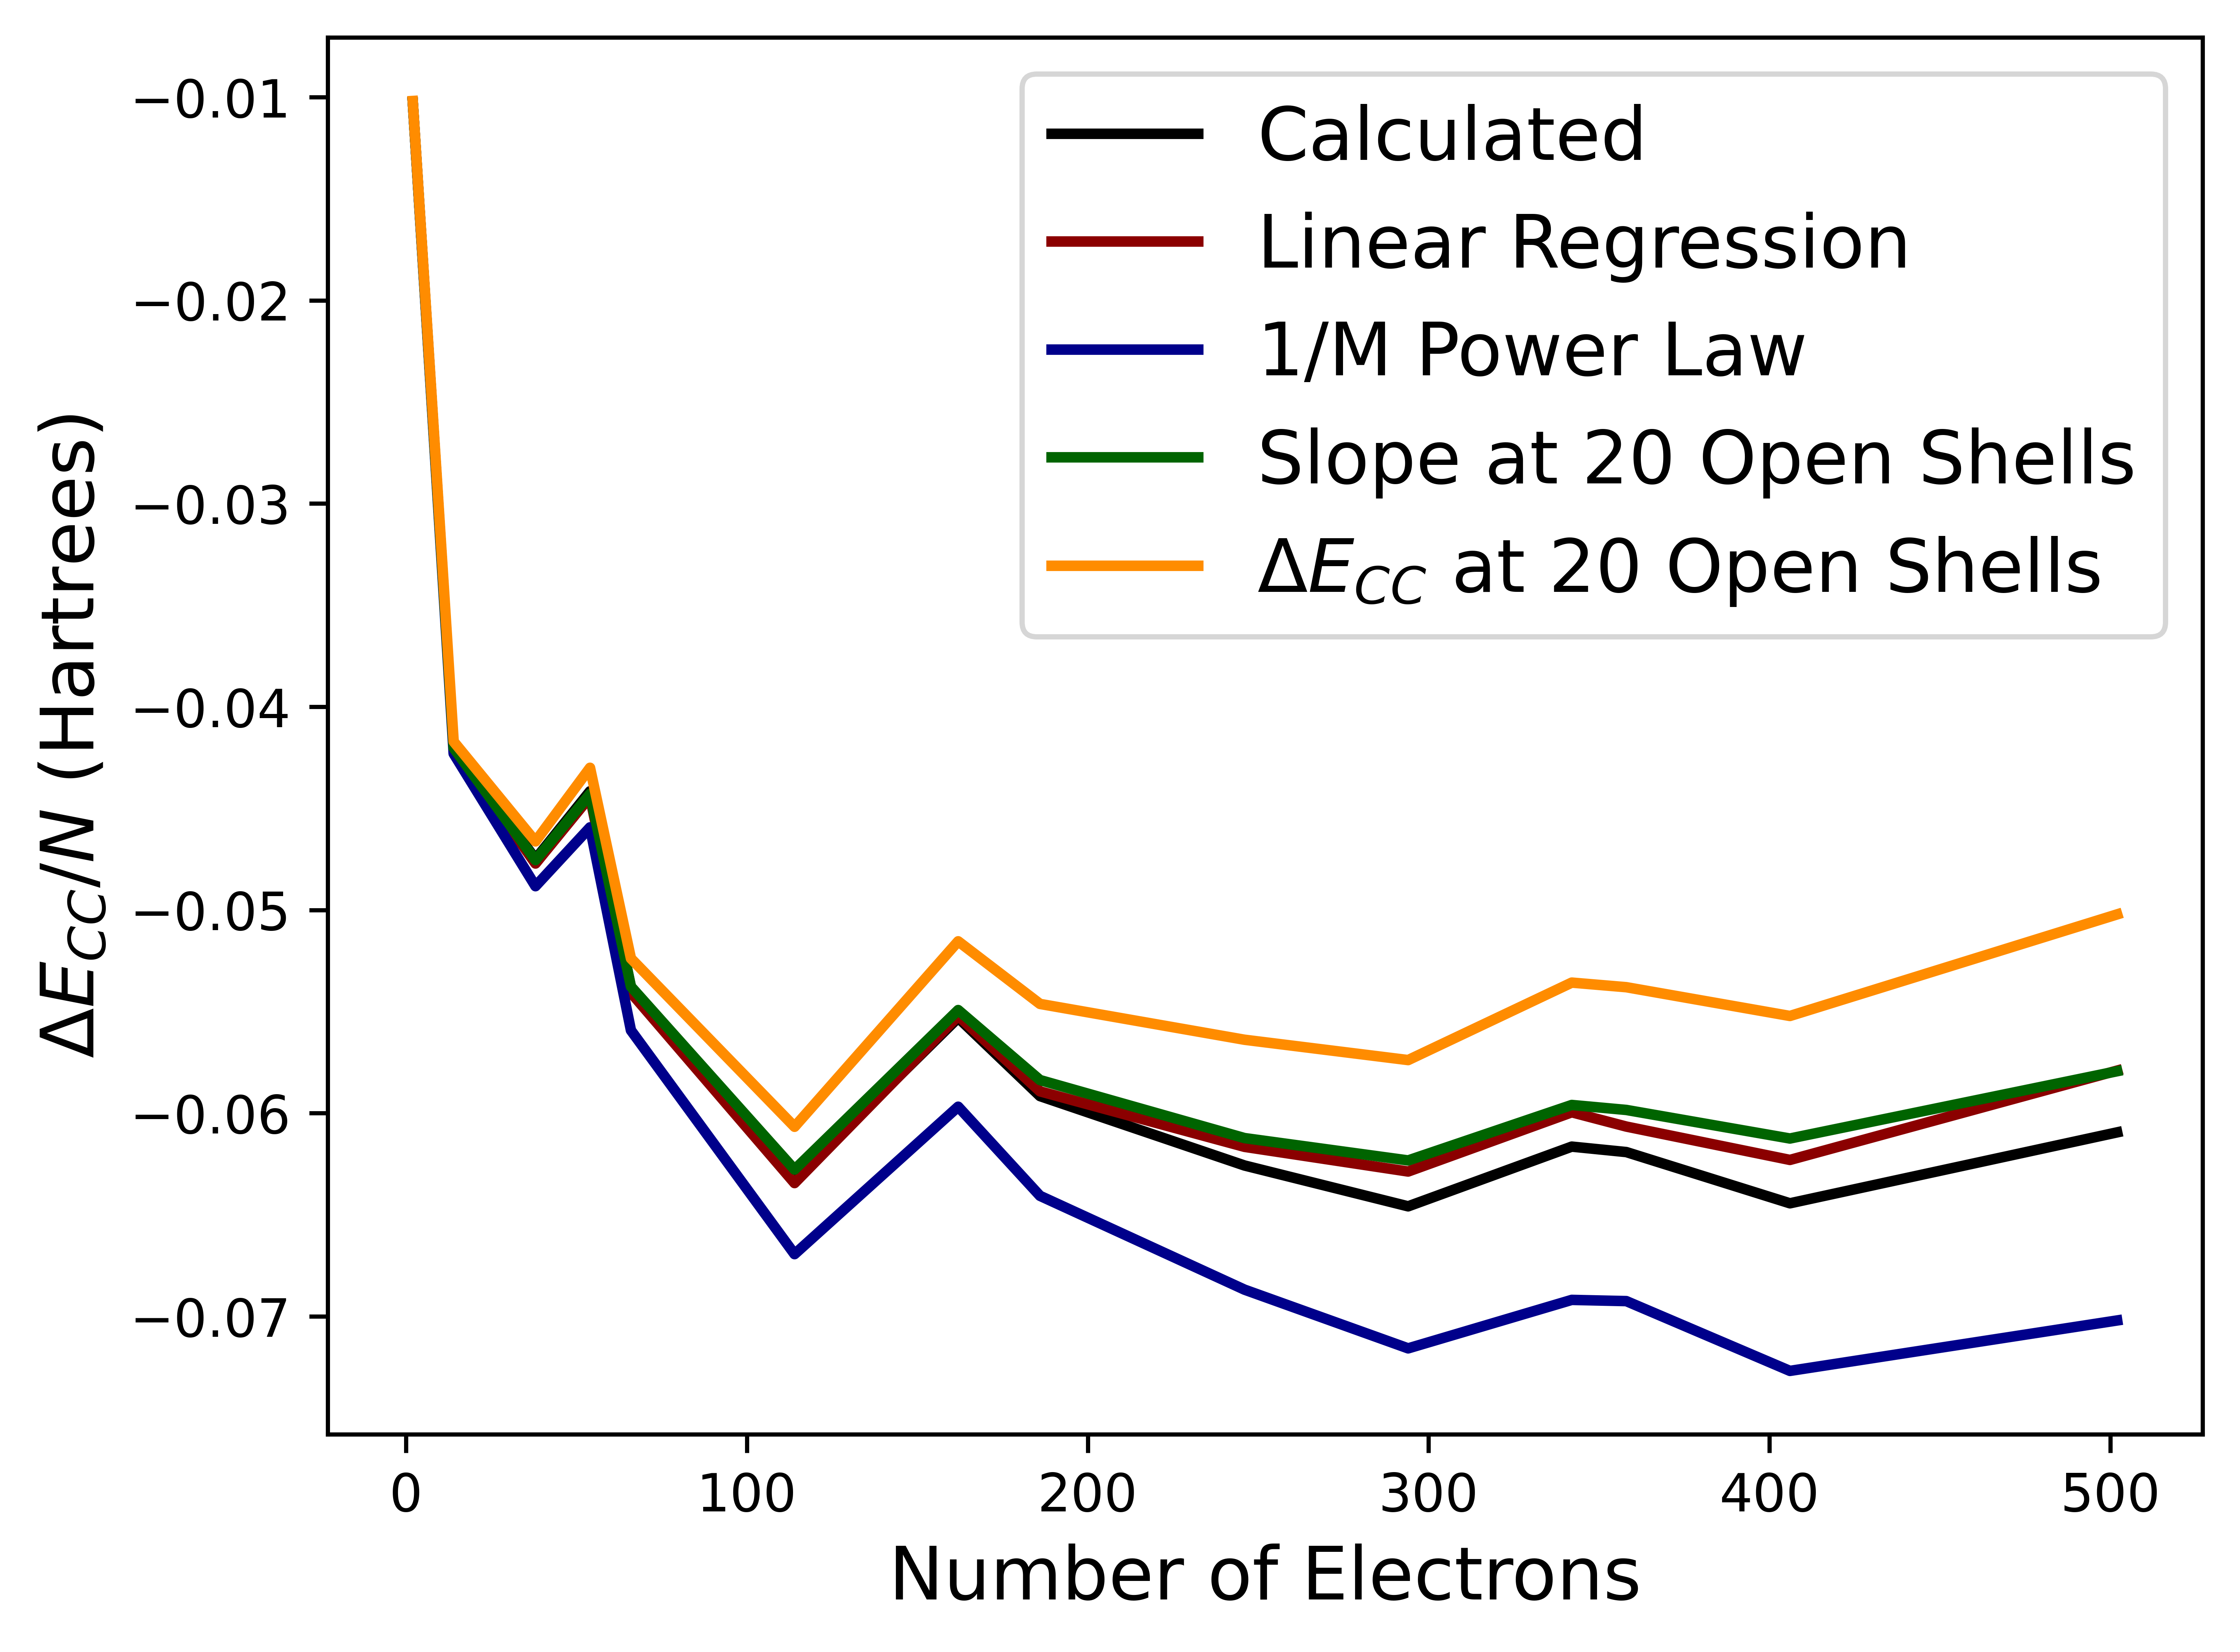
\includegraphics[scale=0.75]{Images/Chapter7/ElectronGas/EG_extrapolation_compare_no_sre.png}
    \caption{The converged CCD correlation energies (black) calculated at M = 6,142 for an HEG with $r_s$ = 0.5.  Also displayed are the results of predicting the converged correlation energies with a truncation at 20 open shells (yellow) which has a percent error of 6.87$\%$, using a 1/M power law (blue) which has an average percent error of 7.00$\%$, using the CCD to MBPT2 slope calculated at 20 open shells (green) which have an average percent error of 1/16$\%$, and using linear regression to model the graph from Fig. \ref{mbpt_vs_cc} (red) which has an average percent error of 0.95$\%$.}
    \label{fig:compare_no_sre}
\end{figure}
    \subsection*{Ridge Regression}

Now that we have looked at performing the basis completeness extrapolations with traditional methods, we can develop a machine learning-based approach. A good machine learning algorithm will have a small number of hyperparameters to tune and give reproducible and accurate results for the extrapolation. Ridge regression only has one hyperparameter and a closed-form solution for its optimized weights. Therefore, it will always train the same way when given the same training data, making it a much more attractive alternative than neural networks, with their many hyperparameters and unrepeatable results.

The ridge regression algorithm contains one hyperparameter, $\alpha$, which is the strength of the regularization. Since this is a hyperparameter, the user must set its value before training the ridge regression algorithm. However, its value can significantly impact the results of the ridge regression. For example, figure \ref{fig:vary_alpha} shows the results of using the SRE algorithm with ridge regression and various $\alpha$ values to predict the converged $\Delta E_{CC}$ energies of the HEG with $r_s$ = 0.5.

\begin{figure}
    \centering
    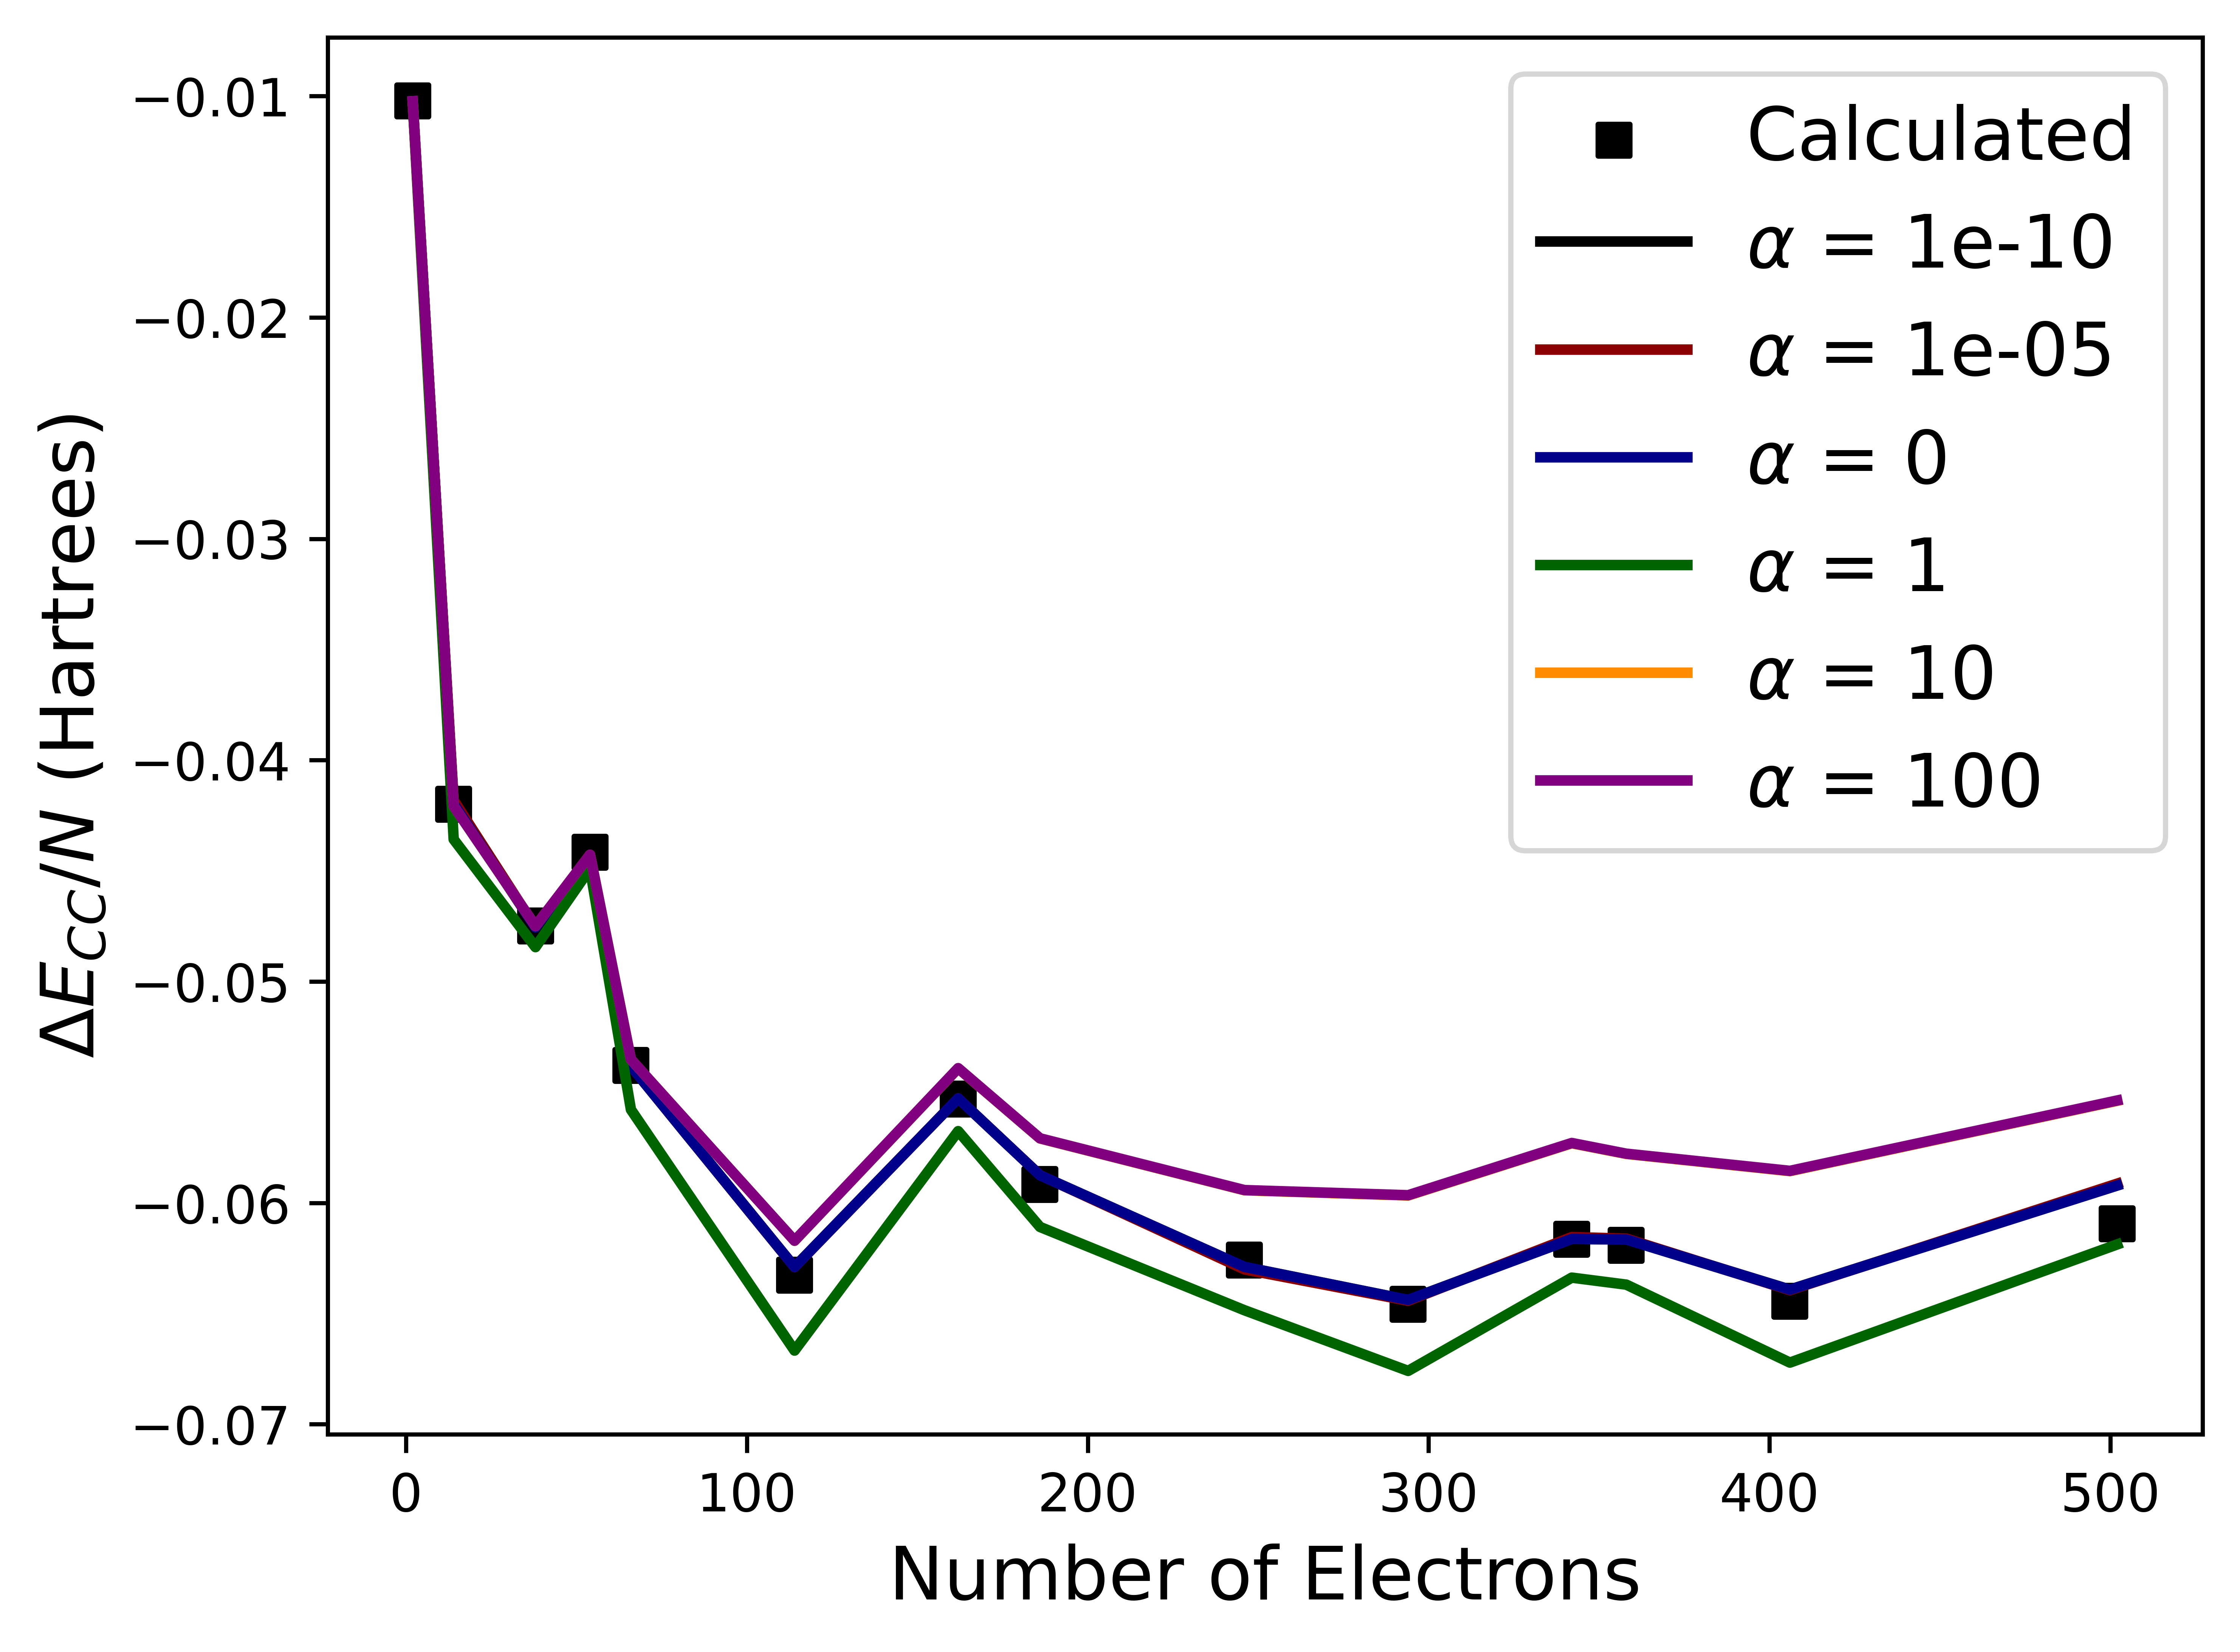
\includegraphics[scale=0.75]{Images/Chapter7/ElectronGas/vary_alpha.png}
    \caption{This figure shows the extrapolations' dependence on the hyperparameter $\alpha$. The results of performing an SRE analysis on the HEG with $r_s$ = 0.5 and at various numbers of electrons. The machine learning algorithm used for the SRE algorithm is ridge regression.}
    \label{fig:vary_alpha}
\end{figure}

For Fig. \ref{fig:vary_alpha}, the training data was chosen to be between 5 and 20 open shells (inclusive) or 2 $\leq$ M $\leq$ 2,090 (exact values of M depend on N). The sequence length for the SRE algorithm was set to 3, and the data set was extrapolated until there were 50 total points and the convergence was confirmed. The value of $\Delta E_{CC}$ we get from this process is considered converged. Therefore we will compare it to converged calculations of the HEG at M = 6,142, where the correlation energy convergence has converged. In Fig. \ref{fig:vary_alpha} $\Delta E_{CC, 6142}$ are plotted with scattered square points. These are considered to be the "true" or most accurate results. The solid lines show the results of performing the SRE algorithm to converge the correlation energy with respect to the number of single-particle states using the SRE algorithm with a variety of values for the hyperparameter $\alpha$.   Note that several of the values of $\alpha$ produce essentially equivalent results, so there are not six distinct lines. For $\alpha$ = 1x10$^{-10}$ and 1x10$^{-5}$ (which provide nearly identical results), the results are very close to the fully calculated converged correlation energies, with the average percent error overall numbers of electrons of 0.49$\%$. However, on the other hand, $\alpha$ = 1 and $\alpha$ = 100 provide results that visually appear to be suitable matches for the expected pattern in the data but do not match the converged calculations. However, if the fully converged calculations were not available for comparison, these could be considered reasonable predictions. For $\alpha$ = 1, the average percent error overall numbers of electrons is 3.09$\%$, and for $\alpha$ = 100, the average percent error is 3.87$\%$. Not shown in Fig. \ref{fig:vary_alpha} are the predictions for $\alpha$ = 1x10$^{-2}$ because the average percent error for the SRE algorithm's predictions and the actual data for this $\alpha$ value is 3.45x10$^{6}$$\%$. While this produces an undeniably incorrect result even if the actual data was not available for comparison, this shows the variation that can happen with the SRE predictions as $\alpha$ varies, and $\alpha$ values both larger and smaller than 1x10$^{-2}$ provide reasonable predictions, but $\alpha$ = 1x10$^{-2}$ provides predictions that do not converge.

A hyperparameter is typically set through a process known as hyperparameter tuning. In hyperparameter tuning, many different values are tested for the hyperparameters to find the best ones. First, the algorithm is defined using a given set of hyperparameters and trained using the training data; then, its accuracy is tested using a validation data set. The validation data set can be a subset of the training data, the test data, or a new data set altogether. This define-train-test cycle is repeated with many combinations of hyperparameters, and the hyperparameters that produce the lowest error on the validation data set are kept for future use.

For the HEG, we have data at five different values of $r_s$, so it was decided to choose one value of $r_s$ for hyperparameter tuning. Therefore, for the chosen value of $r_s$, not only does the SRE training data need to be generated, but the converged correlations energies at M = 6,142 also need to be generated will be a time-consuming process. When performing the hyperparameter tuning process on $\alpha$, 1,000 different values were tested, evenly spaced on a log scale between 1x10$^{-10}$ and 100 (inclusive). For each value, a ridge regression algorithm was defined with that value for $\alpha$. The ridge regression algorithm was used for an SRE analysis using the same training process described above. The predicted values for $\Delta E_{CC}$ were then compared to the fully converged calculations. The value for $\alpha$ that produced the lowest average percent error overall numbers of electrons was kept. This process was performed independently with all five different $r_s$ data sets to see how the results compare. 

When the hyperparameter tuning is performed using the data sets 0.1 $\leq$ $r_s$ $\leq$ 0.75, the optimal alpha value found was 1x10$^{-10}$. However, the hyperparameter tuning is performed on the data set at $r_s$ = 0.05, and the optimal alpha value was found to be 4.27x10$^{-4}$. When $\alpha$ = 1x10$^{-10}$ the average percent error for all $r_s$ values was 0.45$\%$, which is quite good and is a very acceptable error on the actual data for a prediction made with unconverted data. However, when $\alpha$ = 4.27x1-$^{-3}$ the average percent error for all $r_s$ values is 7.5x10$^{11}$$\%$, because some of the predictions do not converge.  When analyzing the results, this would be a wrong prediction, but as seen in Fig. \ref{fig:vary_alpha}, values of $\alpha$ could be chosen that provide seemingly good but incorrect answers. Moving forward with the ridge regression analysis, we will use $\alpha$ = 1x10$^{-10}$.

\begin{figure}
    \centering
    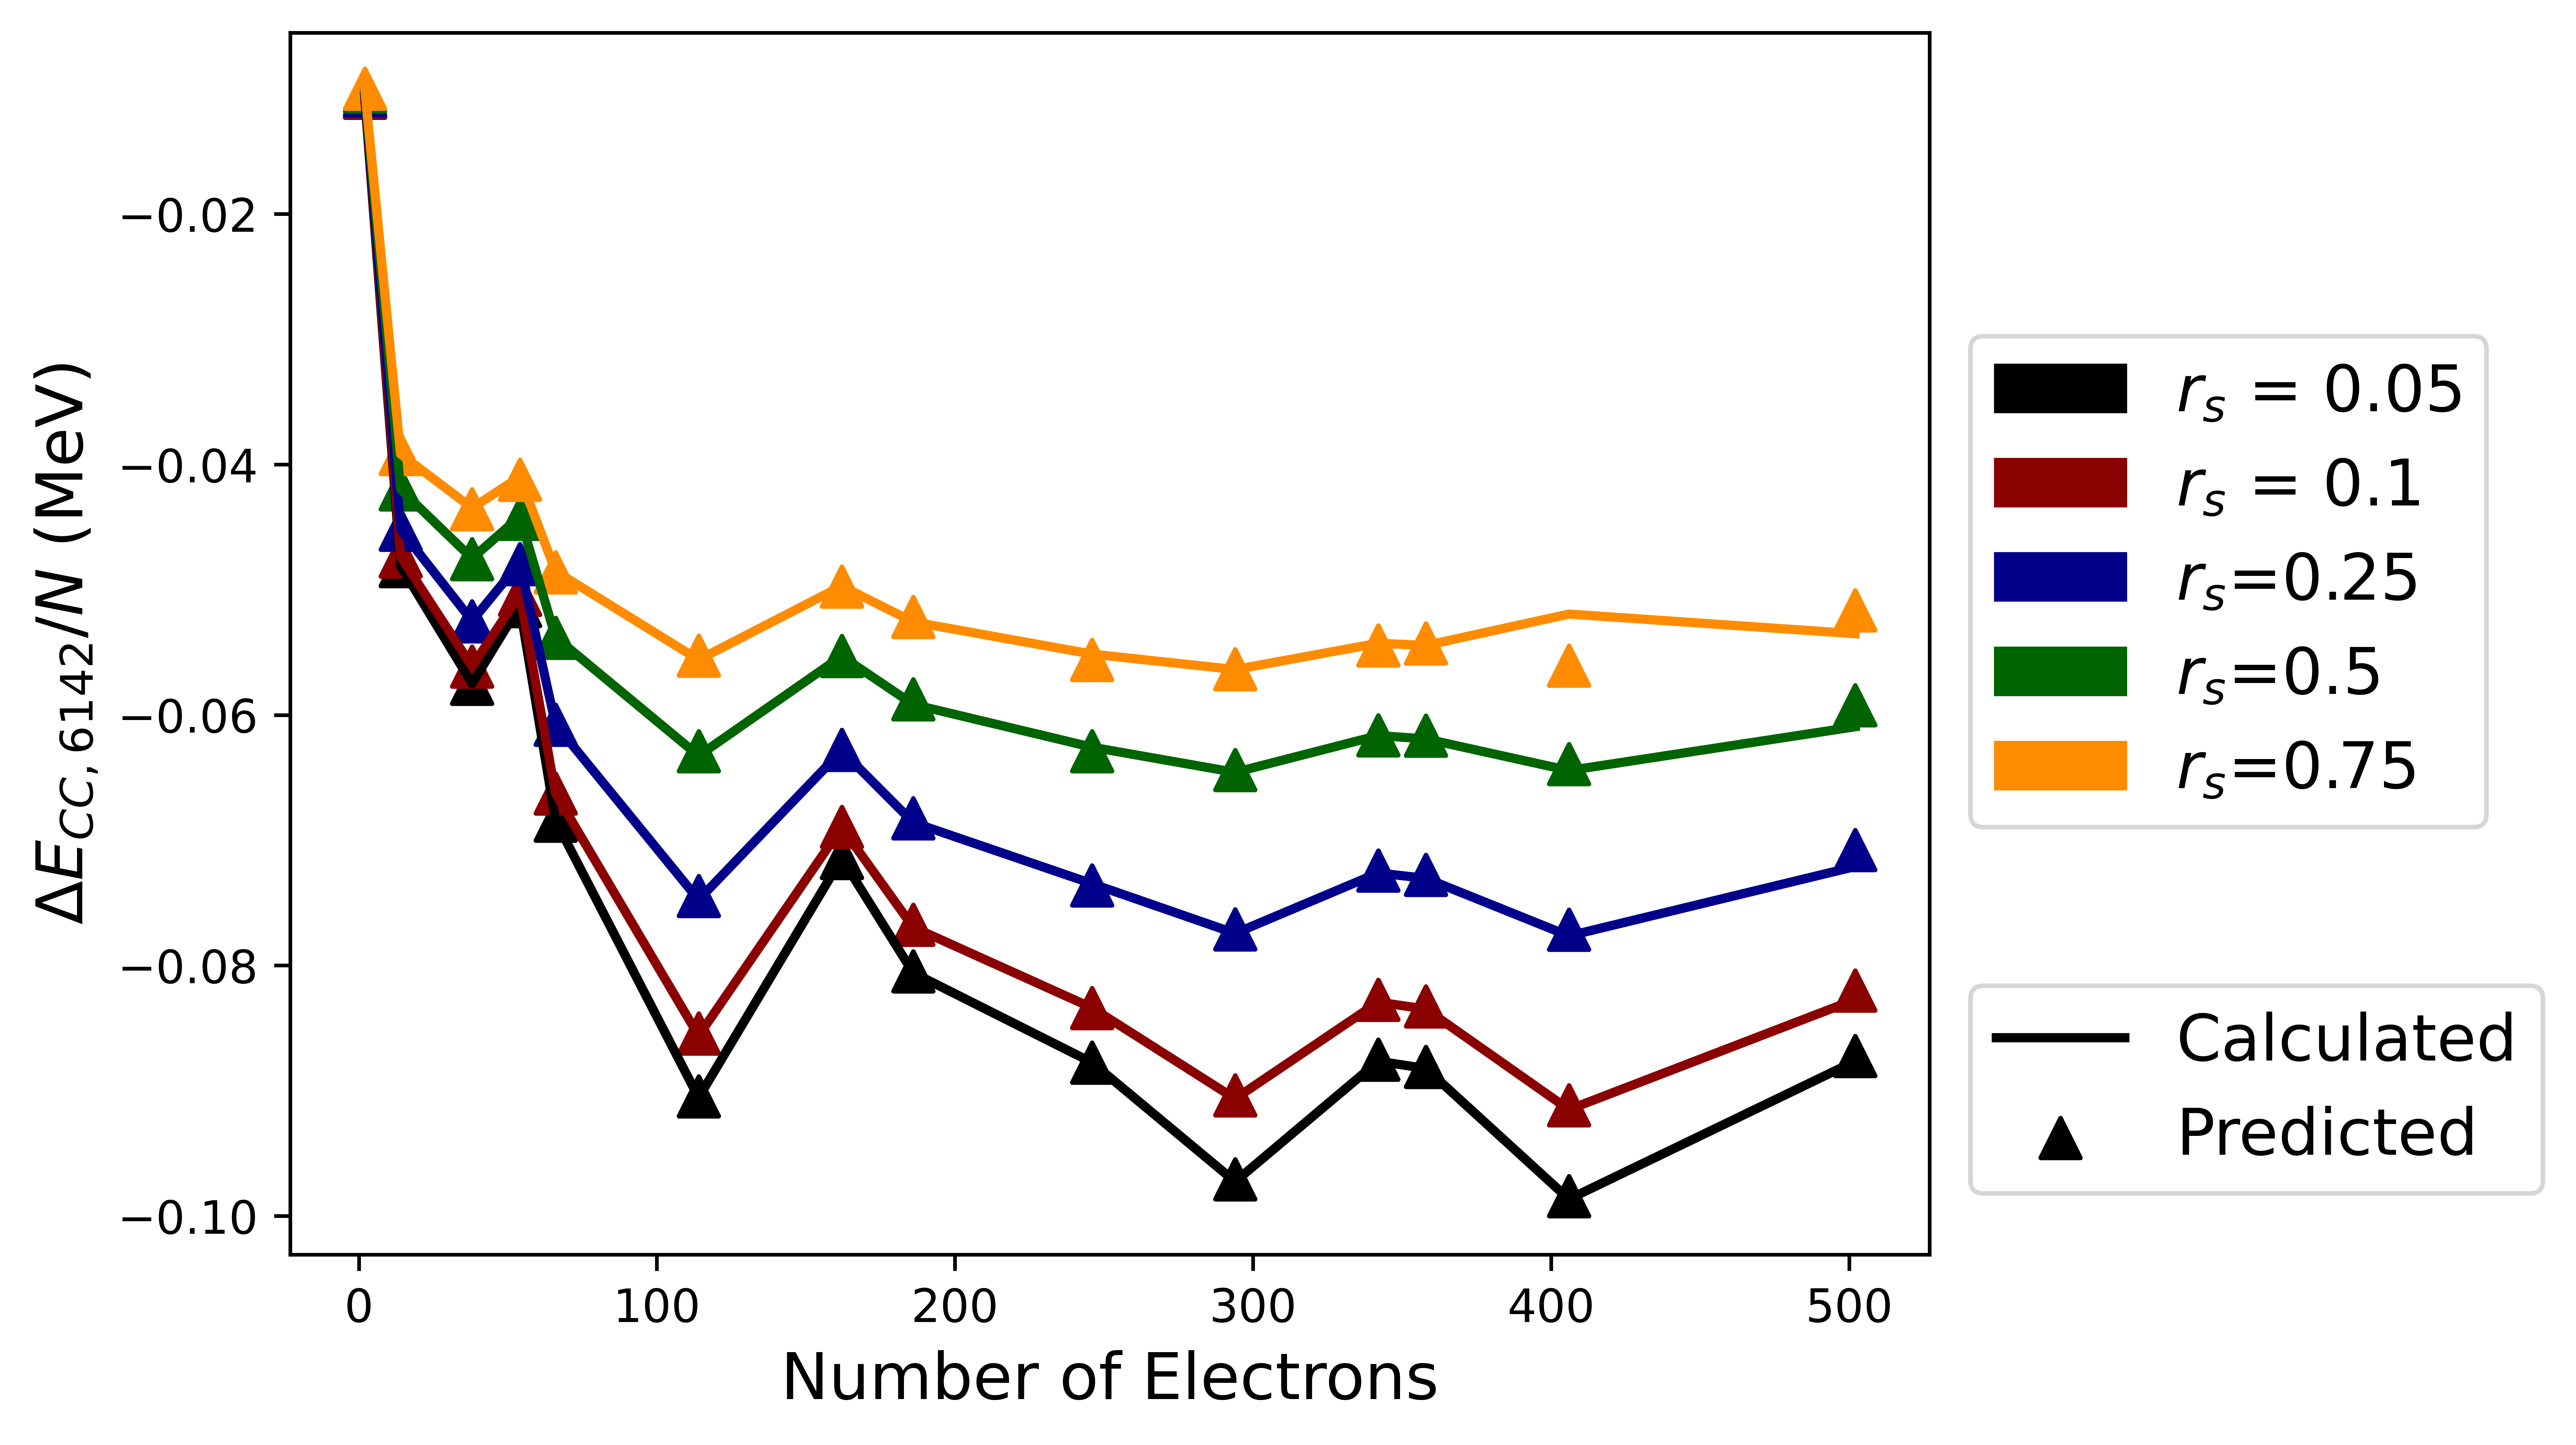
\includegraphics[scale=0.75]{Images/Chapter7/ElectronGas/rs_0_5_EG_Ridge.png}
    \caption{The results of performing an SRE analysis on the HEG to predict the converged CCD correlation energies for 14 different numbers of electrons and five different values of $r_s$.  The SRE predictions, made using a ridge regression algorithm with $\alpha$ = 1x10$^{-10}$, are shown with the triangular markers and the solid lines representing the full correlation energy calculations at M = 6,142. The average percent error between the SRE predictions and the full calculations is 0.45$\%$.}
    \label{fig:rr_tune}
\end{figure}

%% explain rr_tune figure
% 6.88978626138889 10.658995645555557
% 38.32024664305556 54.86648150916667

Fig. \ref{fig:rr_tune} shows the results of performing an SRE analysis on the HEG data set using a ridge regression algorithm with $\alpha$ = 1x10$^{-10}$. This value was chosen because it produces the smallest validation error when performing hyperparameter tuning with the $r_s$ = 0.5 data set. The SRE training procedure was the same as described earlier in this section. The average percent error across all data points in Fig. \ref{fig:rr_tune} is 0.45$\%$, which is tiny. This error is an acceptable level of accuracy of the machine learning predictions, especially considering the potential computational time and resource savings. 

The time needed to generate the training data for the hyperparameter tuning process (i.e., the correlation energies from 5 to 20 open shells for $r_s$ = 0.5) was 6.88 hours. However, the time needed to generate the validation data set (i.e., the correlation energies at M = 6,142 for $r_s$ = 0.5) was 10.65 hours, meaning that the total time needed to generate the data needed for the hyperparameter tuning was 17.53 hours sp there is considerable time to find the optimal value of $\alpha$. If we consider performing the SRE analysis on all five HEG data sets, the time needed to generate all training data is 38.32 hours. Compared to the time needed to generate all $\Delta E_{CC,6142}$ at 54.86 hours, this leads to a time savings for the SRE method of 16.54 hours, or over half a day of computational time saved using the SRE method over doing the complete calculations with no loss of relevant accuracy as the average percent error is less than 0.5$\%$. However, when we add the time needed to generate the validation data set to tune $\alpha$, the time savings drops to only 5.89 hours, which is a much less attractive savings.

%% computational resources discussion

%% Explain the motivation for Bayesian algorithms
Though the SRE algorithm with ridge regression can accurately recreate the converged $\Delta E_{CC}$ for the electron gas at various high densities, the results also display a significant dependence on the hyperparameter $\alpha$ value. Because of this dependence, the fully calculated converged $\Delta E_{CC}$ are not also available, as they are in this work; for comparison, it could be easy to choose a value of $\alpha$ which created a set of converged $\Delta E_{CC}$ which visually look feasible but are not accurate (see Fig. \ref{fig:vary_alpha} for examples). Furthermore, the high computational time and resource requirements needed to generate the validation data set for the hyperparameter tuning process are unattractive. Therefore, we wish to develop a method that can provide the accuracy displayed in Fig. \ref{fig:rr_tune} without dependence and reliance on hyperparameters. Thus, we will start to investigate the Bayesian machine learning implementation of ridge regression: Bayesian ridge regression.

    \subsection*{Bayesian Ridge Regression}

Bayesian ridge regression, the Bayesian machine learning implementation of ridge regression, should be a better choice for the machine learning algorithm for this SRE analysis. Since it is a Bayesian algorithm, it uses Bayesian statistics to find a good value for the hyperparameter, $\alpha$. This means that we do not need to perform hyperparameter tuning or generate a validation data set. Therefore, using Bayesian ridge regression, the only CCD calculations that need to be performed are those for the training data, meaning this method should result in significant time savings between the SRE results and the computing fully converged energies. Additionally, since this is a Bayesian algorithm, it will give us an error in its predictions. Hence, we can get an uncertainty on our converged CCD correlation energy prediction.

This section attempts to predict the CCD correlation energy at M = 6,142 single-particle states (the converged correlation energy) using only the CCD and MBPT2 correlation energies from 5-20 opens shells and the MBPT2 correlation energy at M = 6,142. The exact values of M used in calculating the training data depend on the number of particles in the system but will range from 66 to 2,090 single-particle states. At each of these calculations, the number of single-particle states is not enough to converge the CCD correlation energy, so thus, all of the training data suffers from basis incompleteness errors. Here we will be looking at calculations performed at five different values of $r_s$, so these systems are of a high-density electron gas.

%% SEE DETAILS
Then we used the implementation provided by the Python library Scikit-Learn for Bayesian ridge regression. The SRE sequence length was 2, meaning the Bayesian ridge regression algorithm took two inputs (the previous two ratios of CCD correlation energy to MBPT2 correlation energy). Once the algorithm was trained using the 16 training points, the SRE algorithm was used to extrapolate the ratio until it was converged (resulting in a data set of 50 total points). The final ratio was extracted and multiplied by $\Delta E_{MBPT2, 6142}$ to approximate $\Delta E_{CCD, 6142}$. The analysis results on 14 numbers of electrons and five different $r_s$ values are shown in Fig. \ref{brr_eg}.

%% EXPLAIN THE GRAPH
Fig. \ref{brr_eg} plots the converged CCD correlation energies calculated at M = 6,142 with solid lines. Calculations were performed at 14 different numbers of electrons and five values of $r_s$. Each color in the figure represents a different value of $r_s$. The SRE predictions for each correlation energy are shown with the triangular markers, and the shaded regions represent the uncertainty in the predictions, which comes from the Bayesian ridge regression algorithm. The average percent error for the entire graph is 0.47$\%$.  It should be noted that this is essentially the same result we achieve from the ridge regression analysis with the best value of $\alpha$.

Furthermore, the time needed to generate the SRE training data for all predictions was 289.43 node hours, while the total time needed to generate all energies at M = 6,142 is 200.44 node hours. This leads to a time savings of 88.99 node hours or over 3.5 days of computational time saved with no loss of relevant accuracy. So not only can the SRE method with Bayesian ridge regression accurately predict the converged CCD correlation energies for the HEG across a variety of values of N and $r_s$, but it can also produce uncertainties on its predictions and results in considerable time savings over performing the complete calculations.


\begin{center}
    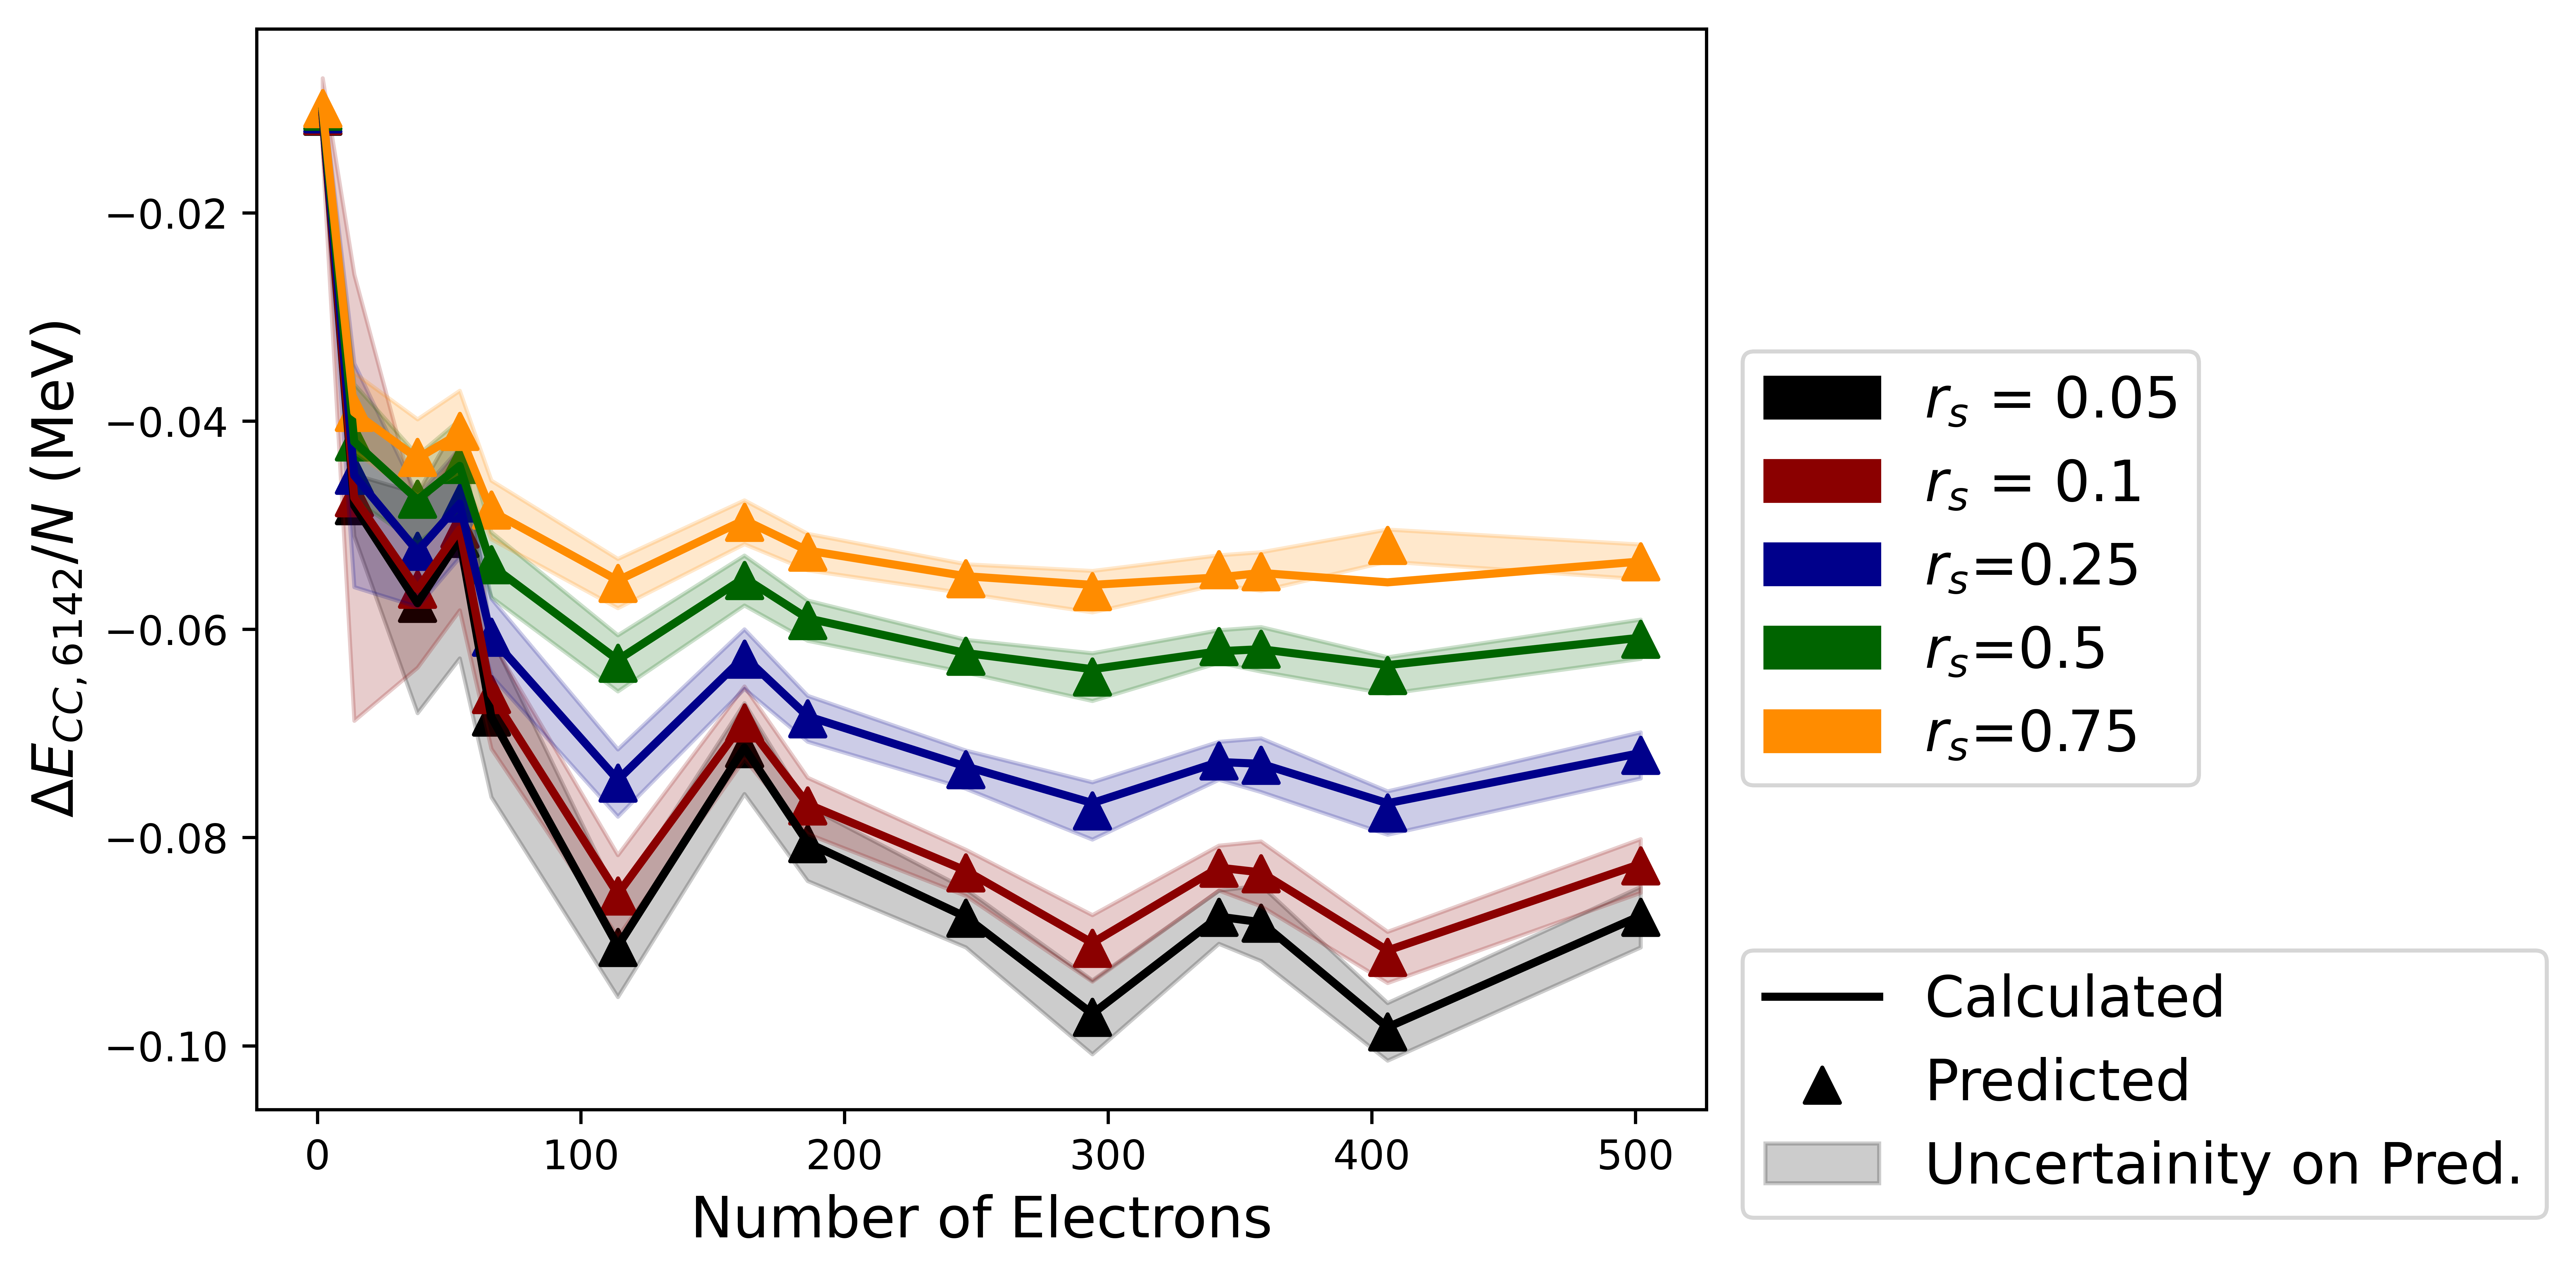
\includegraphics[scale=0.75]{Images/Chapter7/ElectronGas/BRR_EG_MSU_uncertainities.png}
    \captionof{figure}{The results from performing an SRE extrapolation in terms of M for various numbers of electrons and values of r$_s$.  Results are plotted against $\Delta E_{CC,6142}$.}
    \label{brr_eg}
\end{center}


%% ADD SRE TO OTHER EXTRAPOLATIONS
Finally, we can compare the performance of the SRE algorithm to the traditional extrapolation methods we analyzed in Fig. \ref{fig:compare_no_sre}.  For the HEG at $r_s$ = 0.5, if we add the SRE predictions to the others, we get Fig. \ref{fig:compare_sre}.  We can see that the SRE predictions are much closer than any other methods and provide a reasonable approximation to the converged correlation energies, even at high numbers of electrons.

\begin{figure}
    \centering
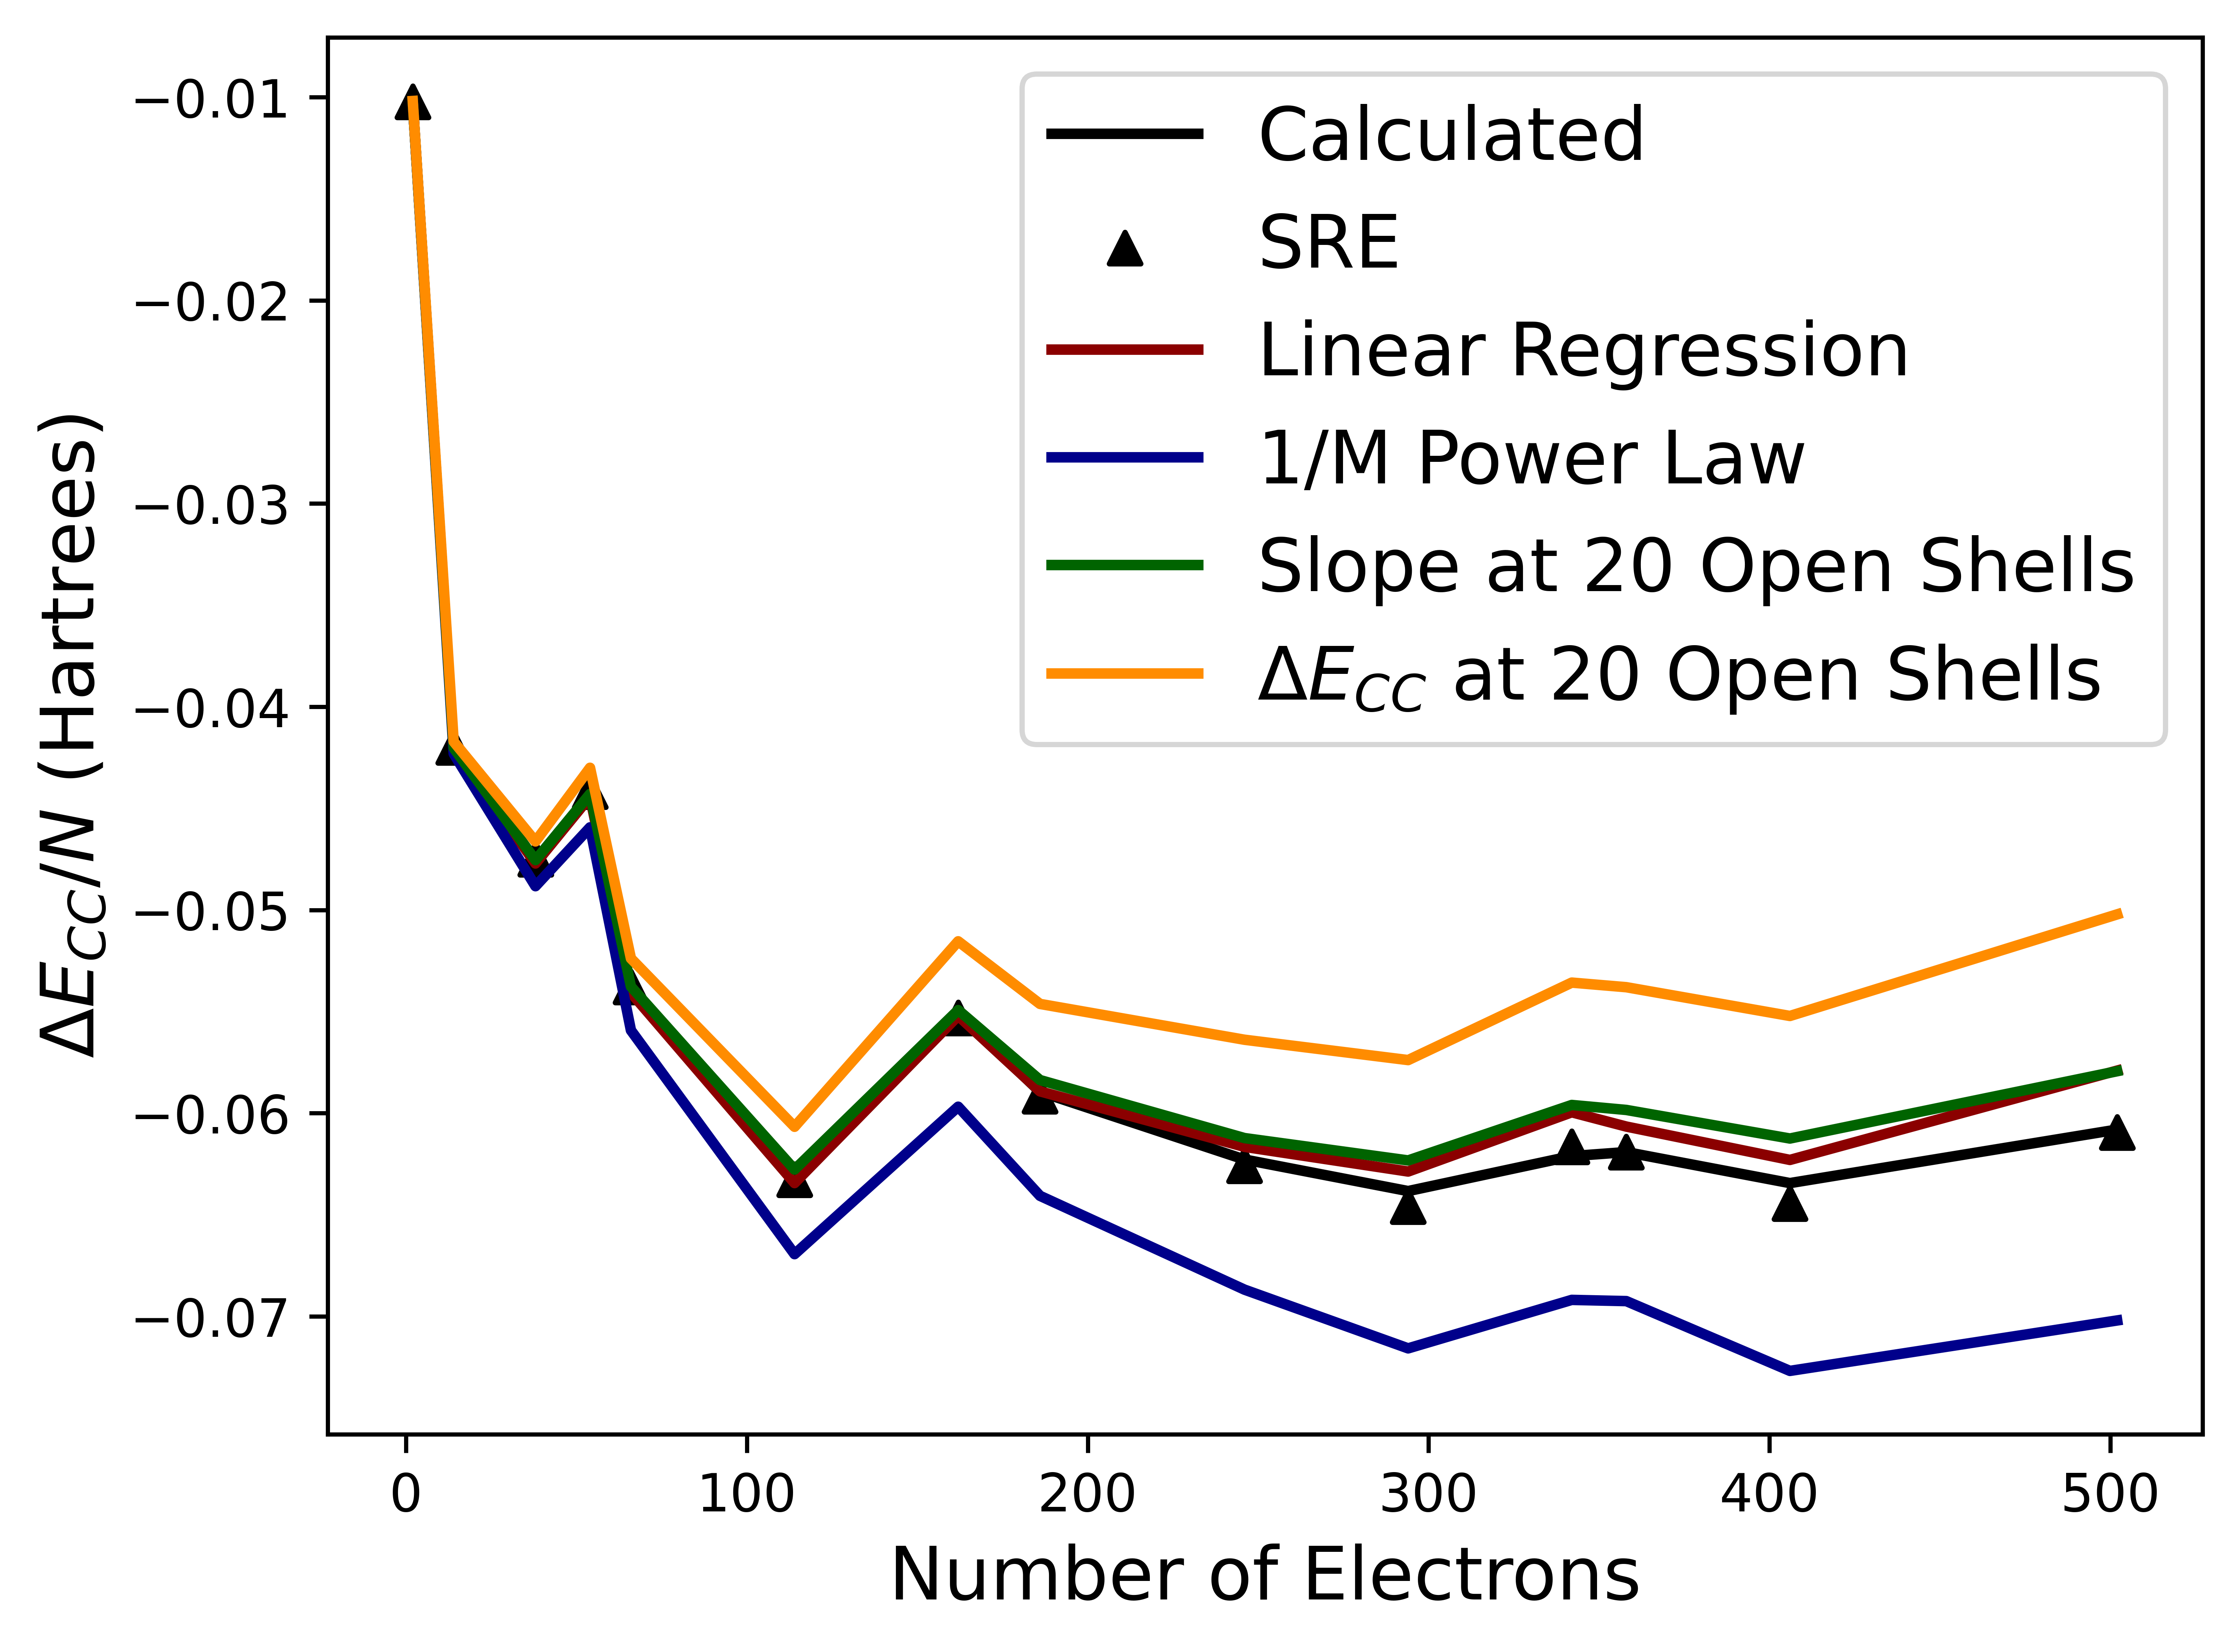
\includegraphics[scale=0.75]{Images/Chapter7/ElectronGas/EG_extrapolation_compare.png}
    \caption{Here, with have recreated Fig. \ref{fig:compare_no_sre}, but have added the SRE results, which have an average percent error of 0.31$\%$.}
    \label{fig:compare_sre}
\end{figure}

%% CONCLUDE
In this section, we have developed the first Bayesian implementation of the SRE method. It has the accuracy of the ridge regression implementation developed in the previous section but without the ambiguity of choosing the algorithm's hyperparameters. Additionally, Bayesian ridge regression provides uncertainties in its predictions, which are helpful in a scientific context. Overall, the SRE method with Bayesian ridge regression is the most promising of the methods attempted so far to remove the basis incompleteness errors.
    \subsection*{Gaussian Process with Rational Quadratic Kernel}

As a final study for the HEG, let us use the Gaussian process (GP) algorithm, another Bayesian machine learning algorithm, as the machine learning component in an SRE analysis. Here we will be using Gaussian processes as the machine learning component of the SRE algorithm. The kernel function will be a modified rational quadratic kernel consisting of a constant kernel multiplied by a rational quadratic kernel and then added to a white kernel. All kernels and the GP algorithm are implemented using the Python library Scikit-Learn.  

As a first study, we will use the same training data set as before, 16 training points taken from between 5 and 20 open shells. We will use an SRE sequence length of three for this training. The only other parameter we set is the $\alpha$ value of the GP algorithm, which we set to $\delta y_{train}^4$, where $\delta y_{train}$ is the standard deviation y component of the training data set. Using the standard deviation when setting $\alpha$ seems to keep the resulting uncertainties small but has little effect on the prediction results.

Fig. \ref{fig:gp_16_points} shows the analysis results on the same data set used in the Bayesian ridge regression section. The average percent error between the SRE predictions for the converged correlation energies and the fully calculated correlation energies at M = 6,142 is 0.73$\%$. While this is larger than the error resulting from the Bayesian ridge regression analysis, it is still tiny and acceptable. Furthermore, it is essential to note that the uncertainties on this, represented by the shaded regions, are significantly smaller than those on the Bayesian ridge regression plot. This is because they are so small in places hidden entirely by the lines!

\begin{figure}
    \centering
    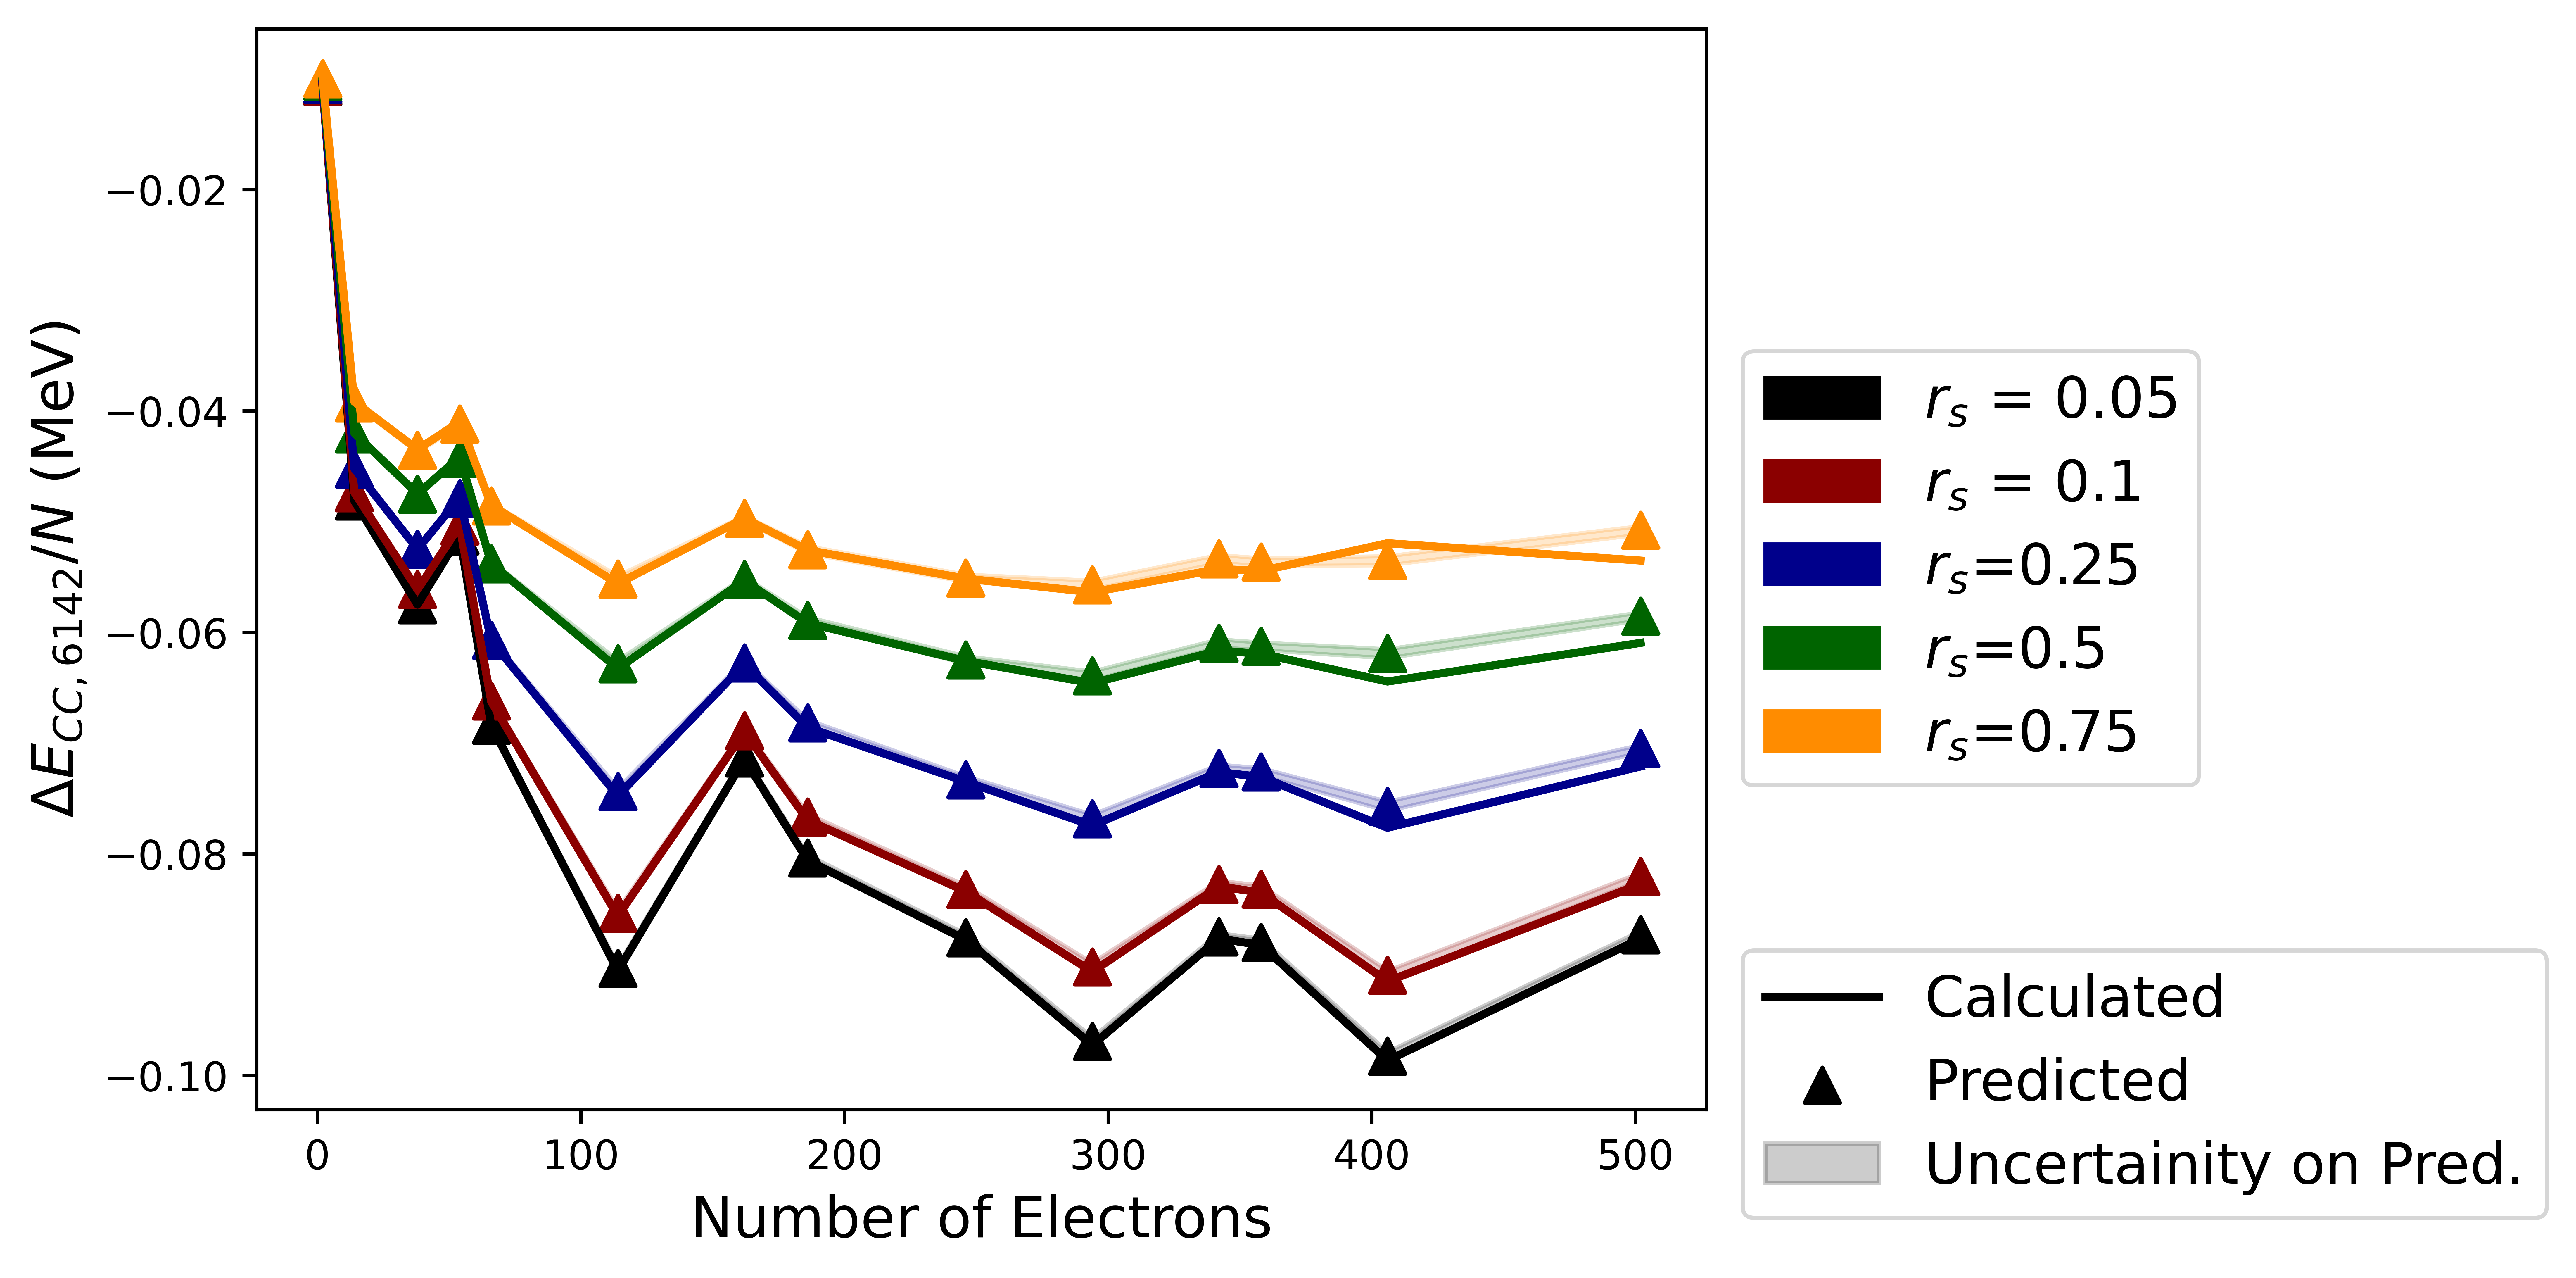
\includegraphics[scale=0.75]{Images/Chapter7/ElectronGas/BRR_EG_MSU_uncertainities-GP.png}
    \caption{The results of performing an SRE analysis with Gaussian processes to predict the converged correlation energies for the HEG at different values of N and $r_s$.  The correlation energies calculated at M = 6,142 are plotted with a solid line and are taken to be the true results, the SRE predictions are plotted with triangular markers, and the shaded region represents the uncertainty on the SRE predictions.}
    \label{fig:gp_16_points}
\end{figure}


As a final analysis with the SRE method on the HEG, we will again use GP as the machine learning algorithm but will reduce the number of training points from 16 to only 10. Here we will use data collected from 5 to 14 open shells, thus removing the six training points with the highest number of single-particle states (and thus the highest computational costs). Here we have also reduced the SRE sequence length to 1 as there are a few training points.

The results of performing this analysis are shown in Fig. \ref{fig:gp_10_points}, using the same plotting scheme as \ref{fig:gp_16_points}. The lower number of training points does lead to a higher average percent error of 1.16$\%$, but this is still a relatively low error, and it does appear, based on the results graph, that most of that error is concentrated in the last two points of the $r_s$ = 0.75 data set.

Next, we must point out the time savings we have gained by reducing the number of training points. When using 16 training points, the time savings is 88.99 node hours, which is not an insignificant amount of time saved. However, with only ten training points, and since the six training points we have removed have the most significant computational time, with this analysis, the amount of computational time saved is 224.43 node hours. That is equivalent to over a week in computational time saved for an error of only 1.16$\%$!

Finally, we justify using the Gaussian processes as the machine learning algorithm over Bayesian ridge regression when there is a small amount of training data. For example, suppose we were to perform this same analysis with Bayesian ridge regression, using ten training points and a sequence length of 1. In that case, the average percent error across all the correlation energies is 6.05$\%$, much higher than the 1.16$\%$ we see with GP. Thus, the GP algorithm works better with smaller data sets and will be the primary algorithm we will use in the next chapter to analyze the infinite nuclear matter, as no training set in that chapter will contain more than 10 points.

\begin{figure}
    \centering
    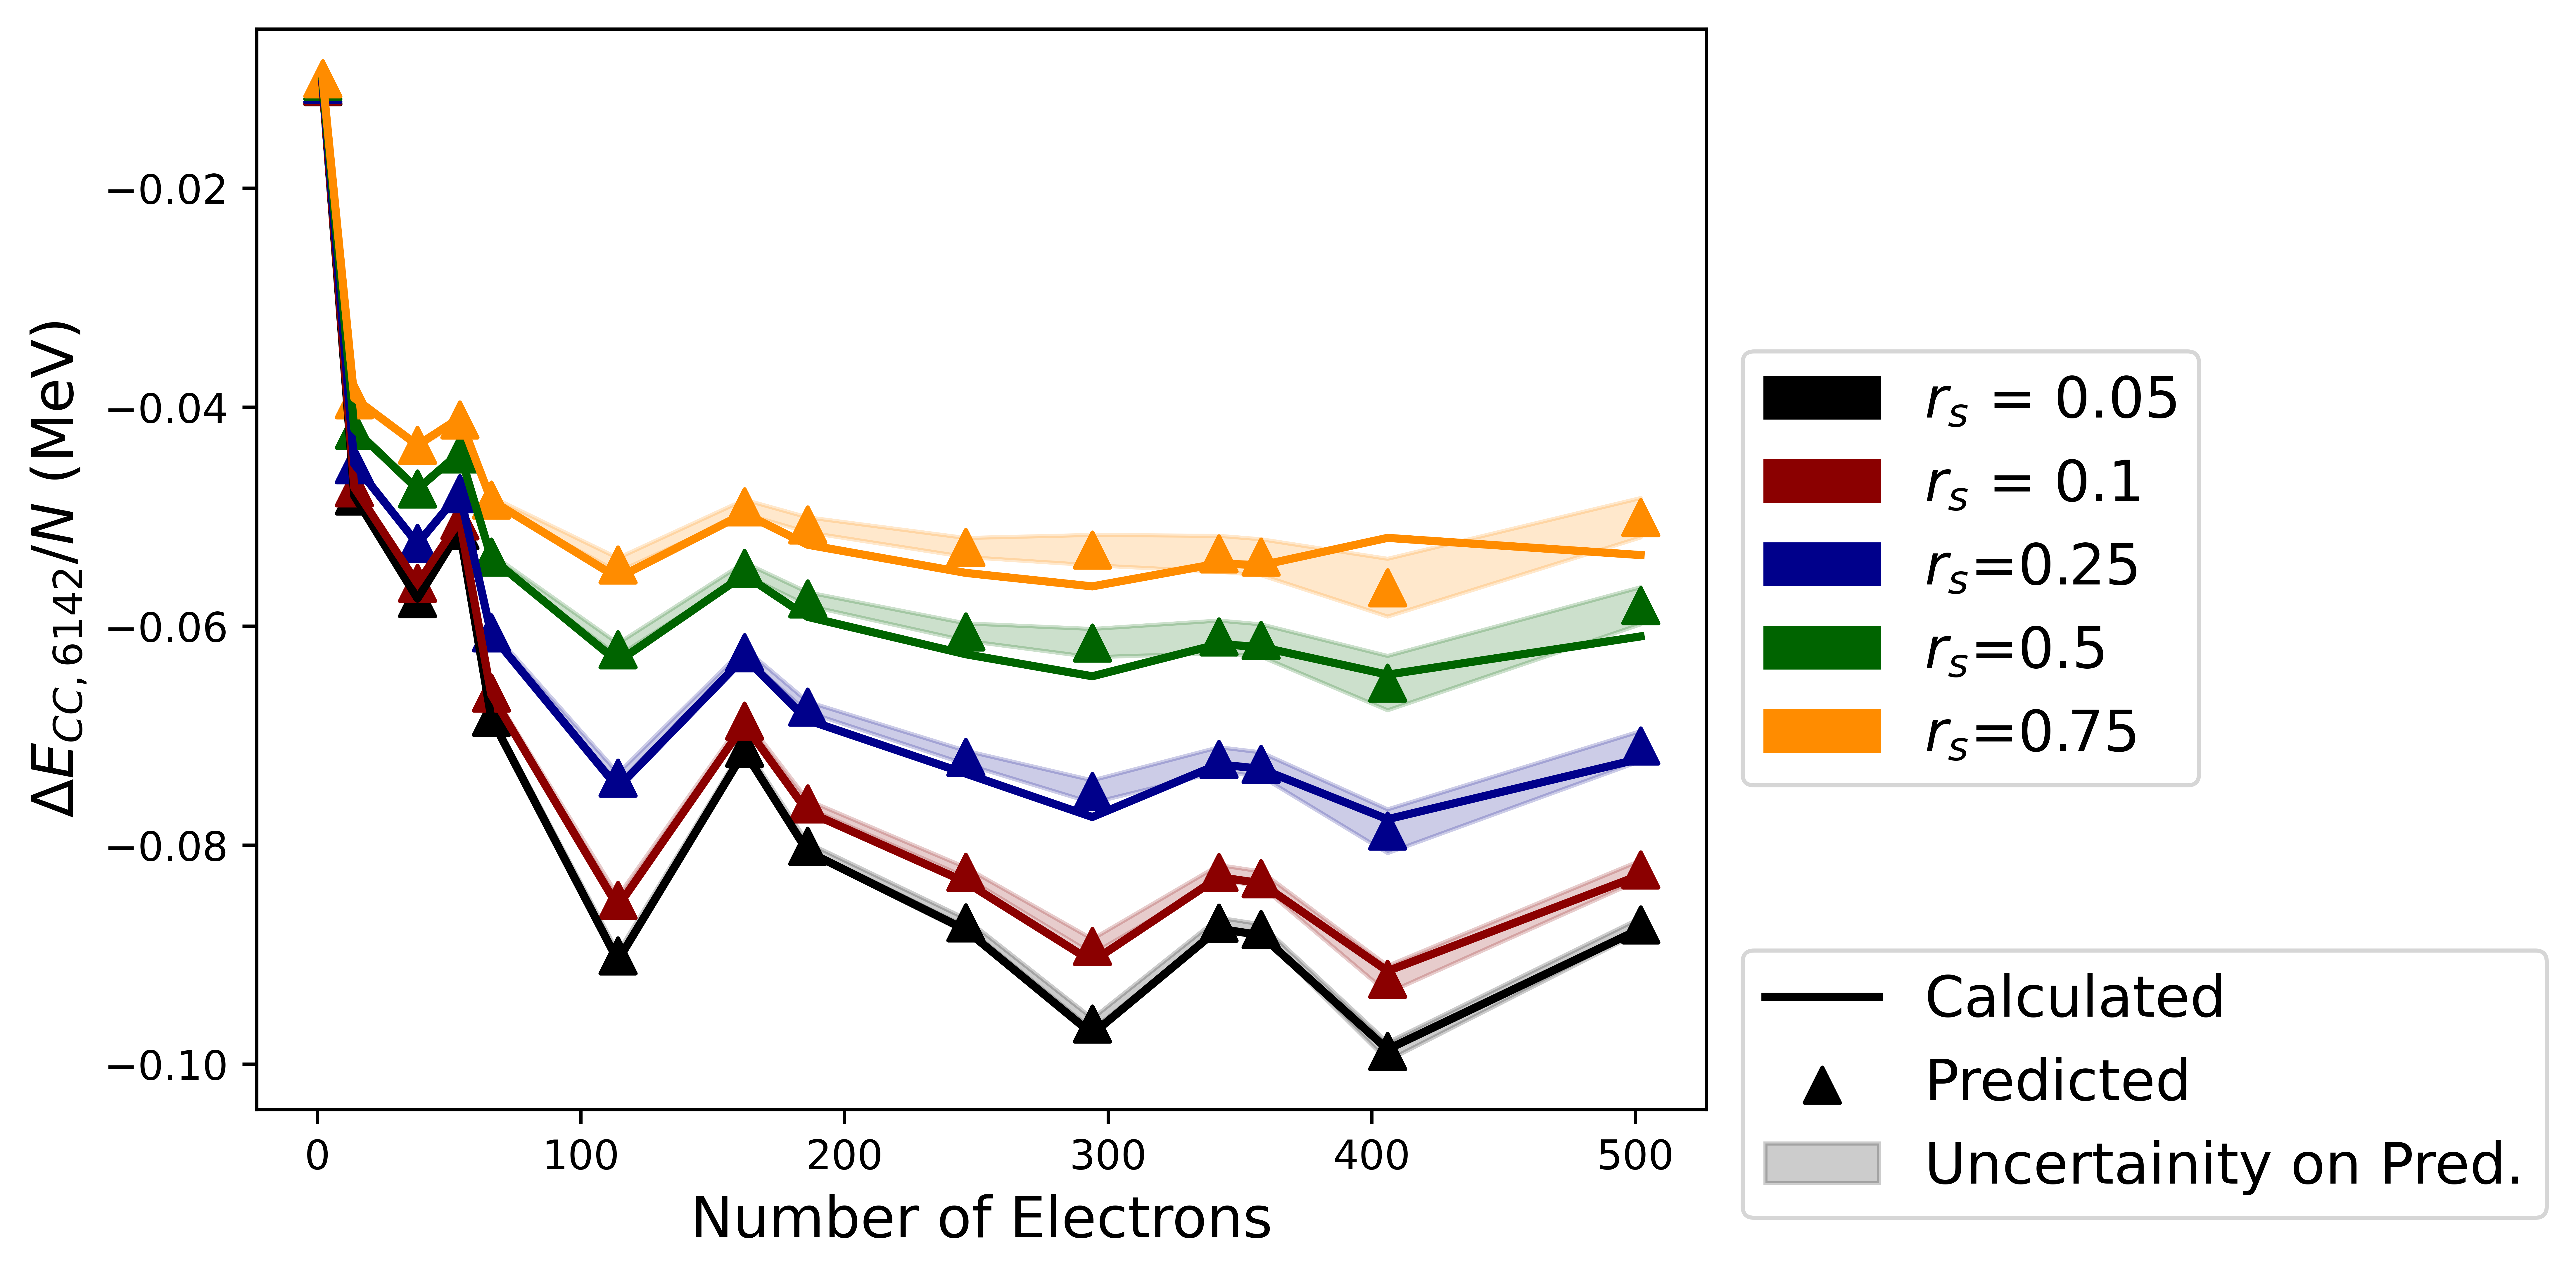
\includegraphics[scale=0.75]{Images/Chapter7/ElectronGas/BRR_EG_MSU_uncertainities_GP_2.png}
    \caption{The results of performing an SRE analysis with Gaussian processes to predict the converged correlation energies for the HEG at different values of N and $r_s$ and only ten training points.  The correlation energies calculated at M = 6,142 are plotted with a solid line and are taken to be the true results, the SRE predictions are plotted with triangular markers, and the shaded region represents the uncertainty on the SRE predictions.}
    \label{fig:gp_10_points}
\end{figure}
    As a final look at the HEG, we can attempt to calculate the correlation energy per electron in the thermodynamic limit using the formalism developed in the previous chapter. We have used 14 training points, from N = 2 to N = 502, and an SRE sequence length of 3. Again, the machine learning algorithm used to make these predictions is the Bayesian Ridge regression algorithm. We attempted this extrapolation using the correlation energies, which have been fully calculated at M = 6,142, and the correlation energies, which have been predicted by the SRE method and are shown in Fig. \ref{brr_eg}.  However, these two extrapolations result in identical correlation energies, with a percent error between the two extrapolated data sets being 0.0$\%$. Thus, there is no reason to use the fully calculated data to predict the TDL correlation energies when the SRE predictions result in the same answer and yield significant time savings.

Fig. \ref{fig:TDL_all} shows the correlation energies per particle for the HEG at a variety of values for N and $r_s$ with solid lines. The horizontal dashed lines show the correlation energy at the TDL as predicted by the SRE algorithm. Even though the correlation energies show significant oscillations with respect to the number of electrons in the system (likely due to the periodic boundary conditions), the SRE predictions seem to provide a suitable match for where the oscillations will converge.

\begin{figure}
    \centering
    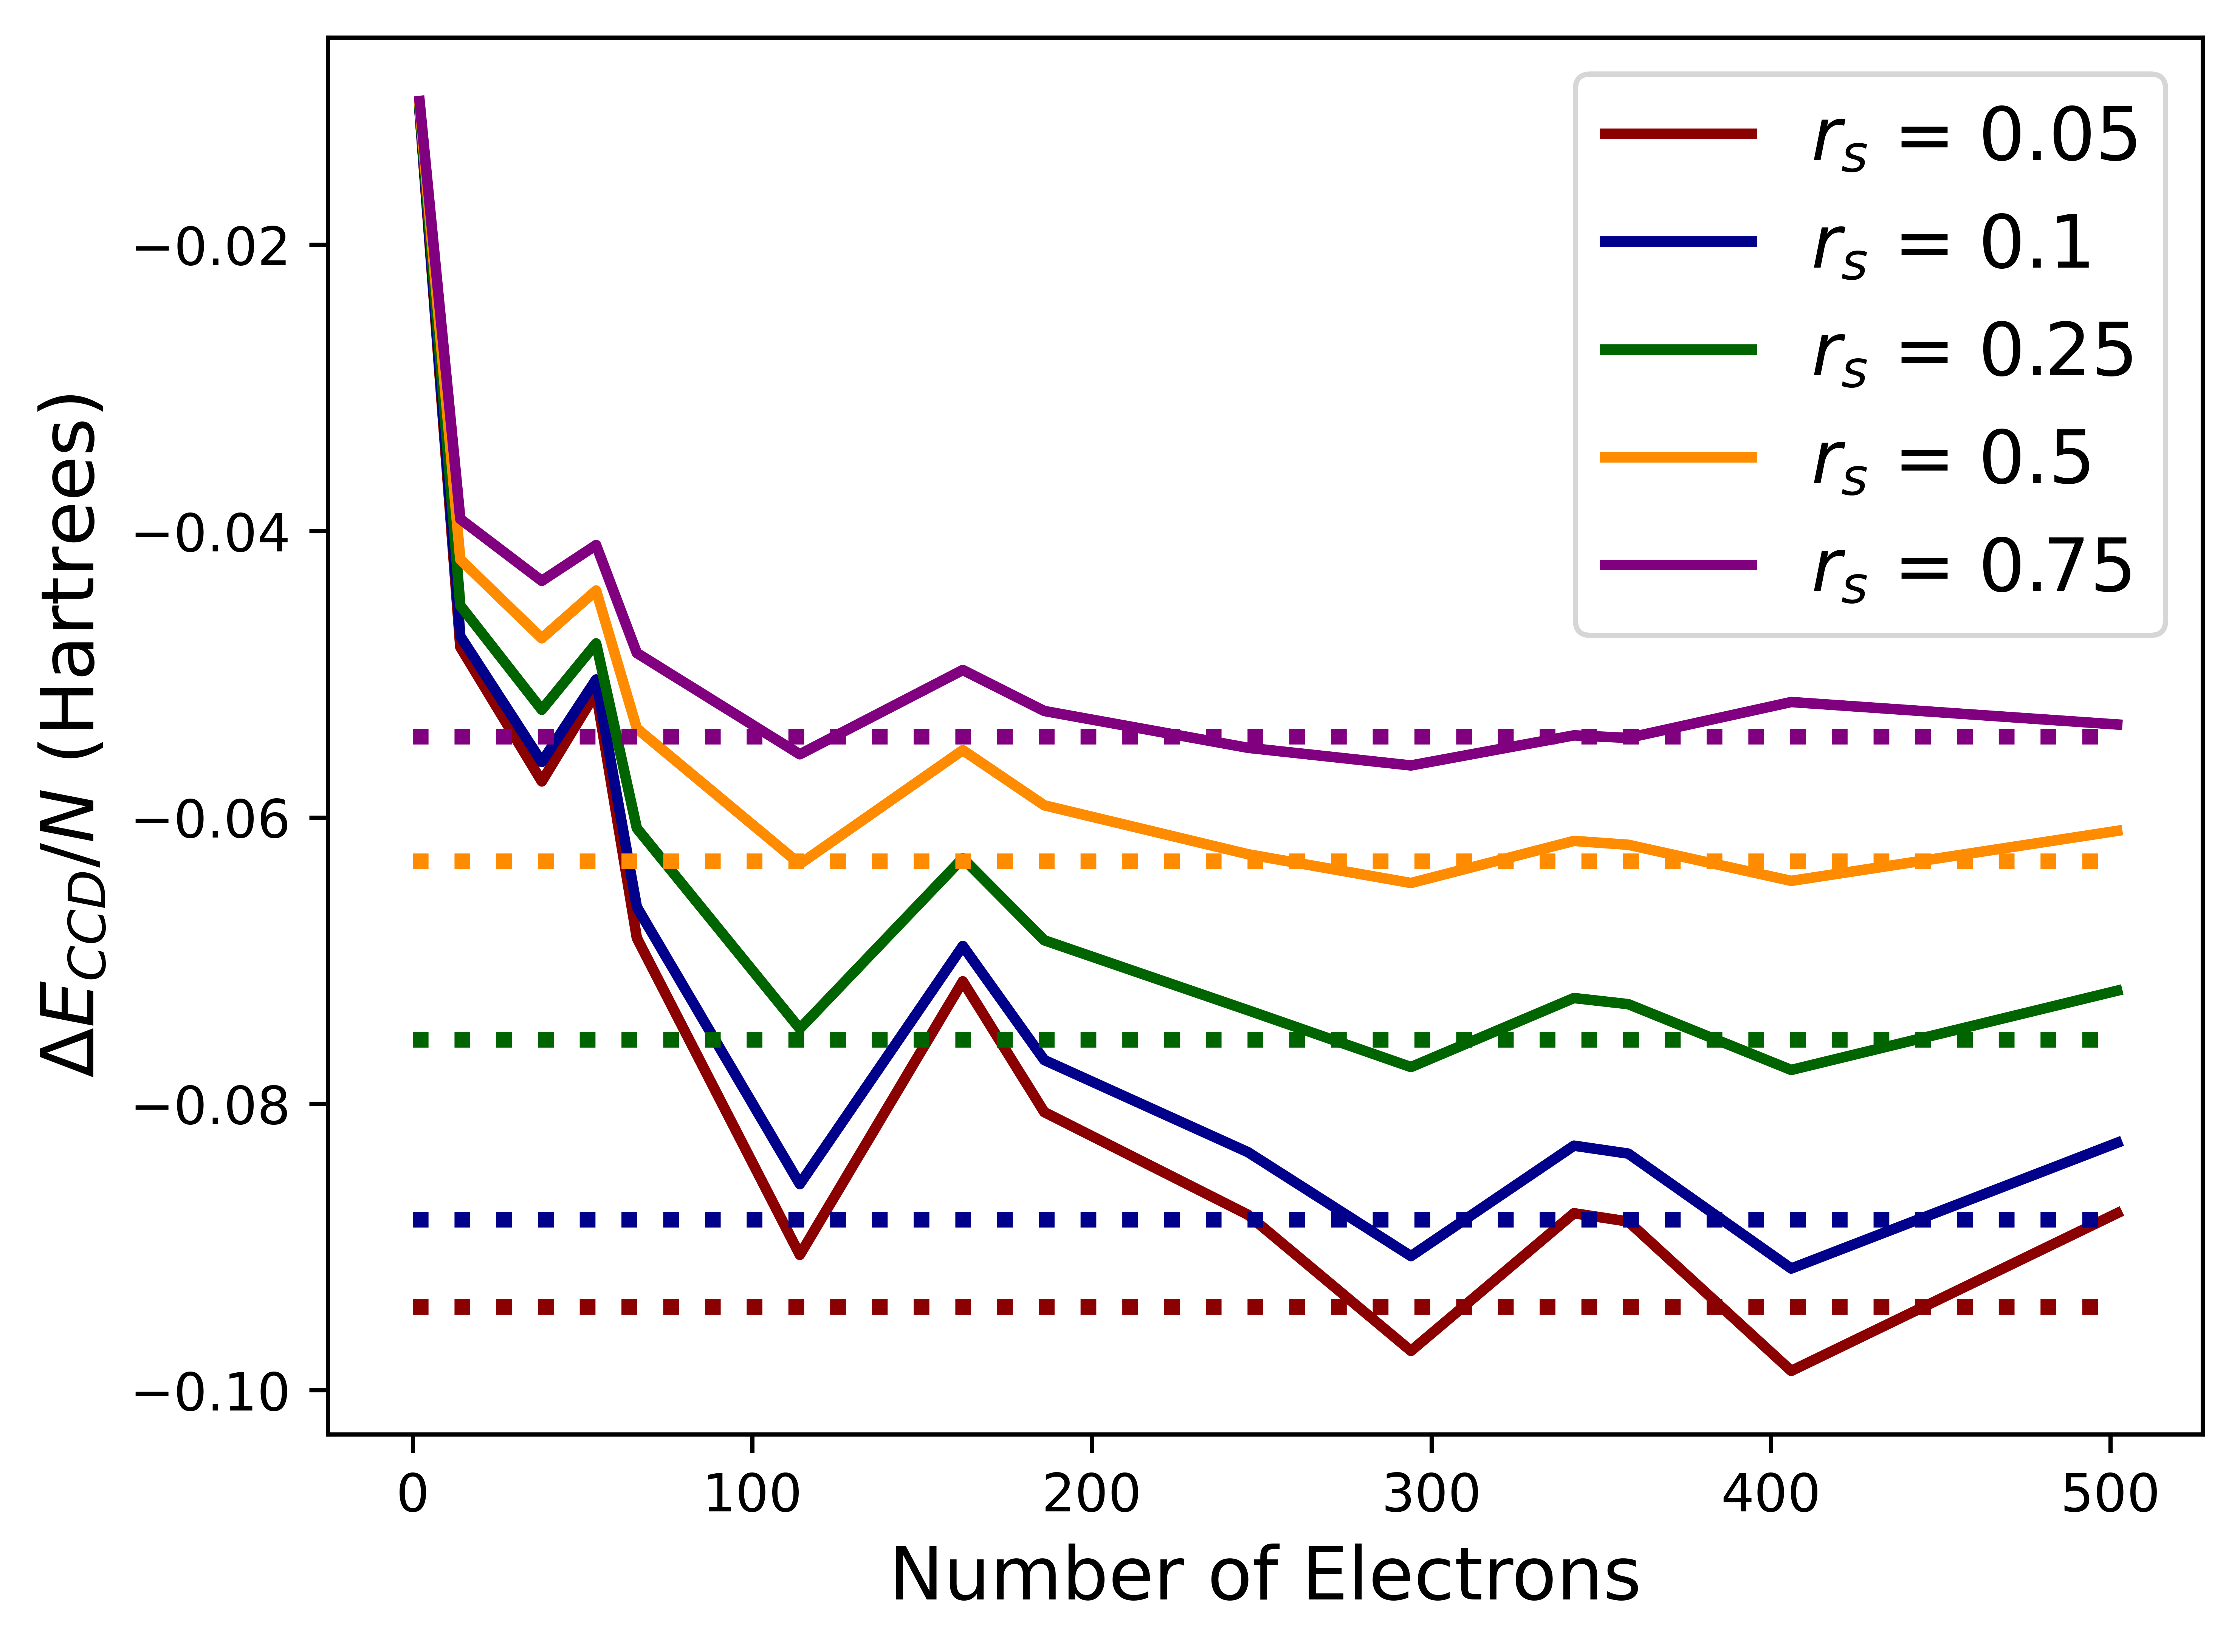
\includegraphics[scale=0.75]{Images/Chapter7/ElectronGas/TDL_all.png}
    \caption{The converged CCD correlation energies for the HEG calculated at M = 6,142 (solid) and the TDL predictions for the correlation energy per particle calculated through the SRE method (dashed).}
    \label{fig:TDL_all}
\end{figure}

While there do exist literature values for the HEG in the TDL (for example, see the work by Bishop et al. in \cite{Ref71} and \cite{Ref72}), the results are highly dependent on the many-body method used, the values of $r_s$ studies, and the specifications of the HEG system. Thus we could not find any currently published literature results to compare our predictions for the exact specifications we have reported. However, we can use a power law, a standard method to find the TDL energies (see Ref. REFERENCE HERE). Therefore, we will use a power law of the form:

\begin{equation}
    \Delta E_{CCD}(N) = \Delta E_{CCD}^\infty + AN^{-\alpha},
\end{equation}

where $\Delta E_{CCD}^\infty$, A, and $\alpha$ are parameters that are fit using data generated at finite numbers of electrons and $\Delta E_{CCD}^\infty$ the is correlation energy at the thermodynamic limit. Usually, $\alpha$ is fixed to 1, which is used when calculating the correlation energy for the system at the TDL. We, however, are interested in calculating the correlation energy in the TDL per electron and thus will leave $\alpha$ unfixed. The results for performing this power law fit are shown in Fig. \ref{fig:TDL_0_5} for a HEG with $r_s$ = 0.5 and are also plotted with the SRE predictions for the correlation energy at the TDL from complete calculations and the SRE predictions. Also shown are the complete calculations for the finite numbers of electrons shown at M = 6,142. While it is impossible to say which of these results is the most accurate, it does appear that the SRE predictions visually provide a better matching for the convergence of the correlation energies in the TDL. However, the best method of predicting the correlation energies in the TDL and the error in the predictions is still a topic of ongoing research.


\begin{figure}
    \centering
    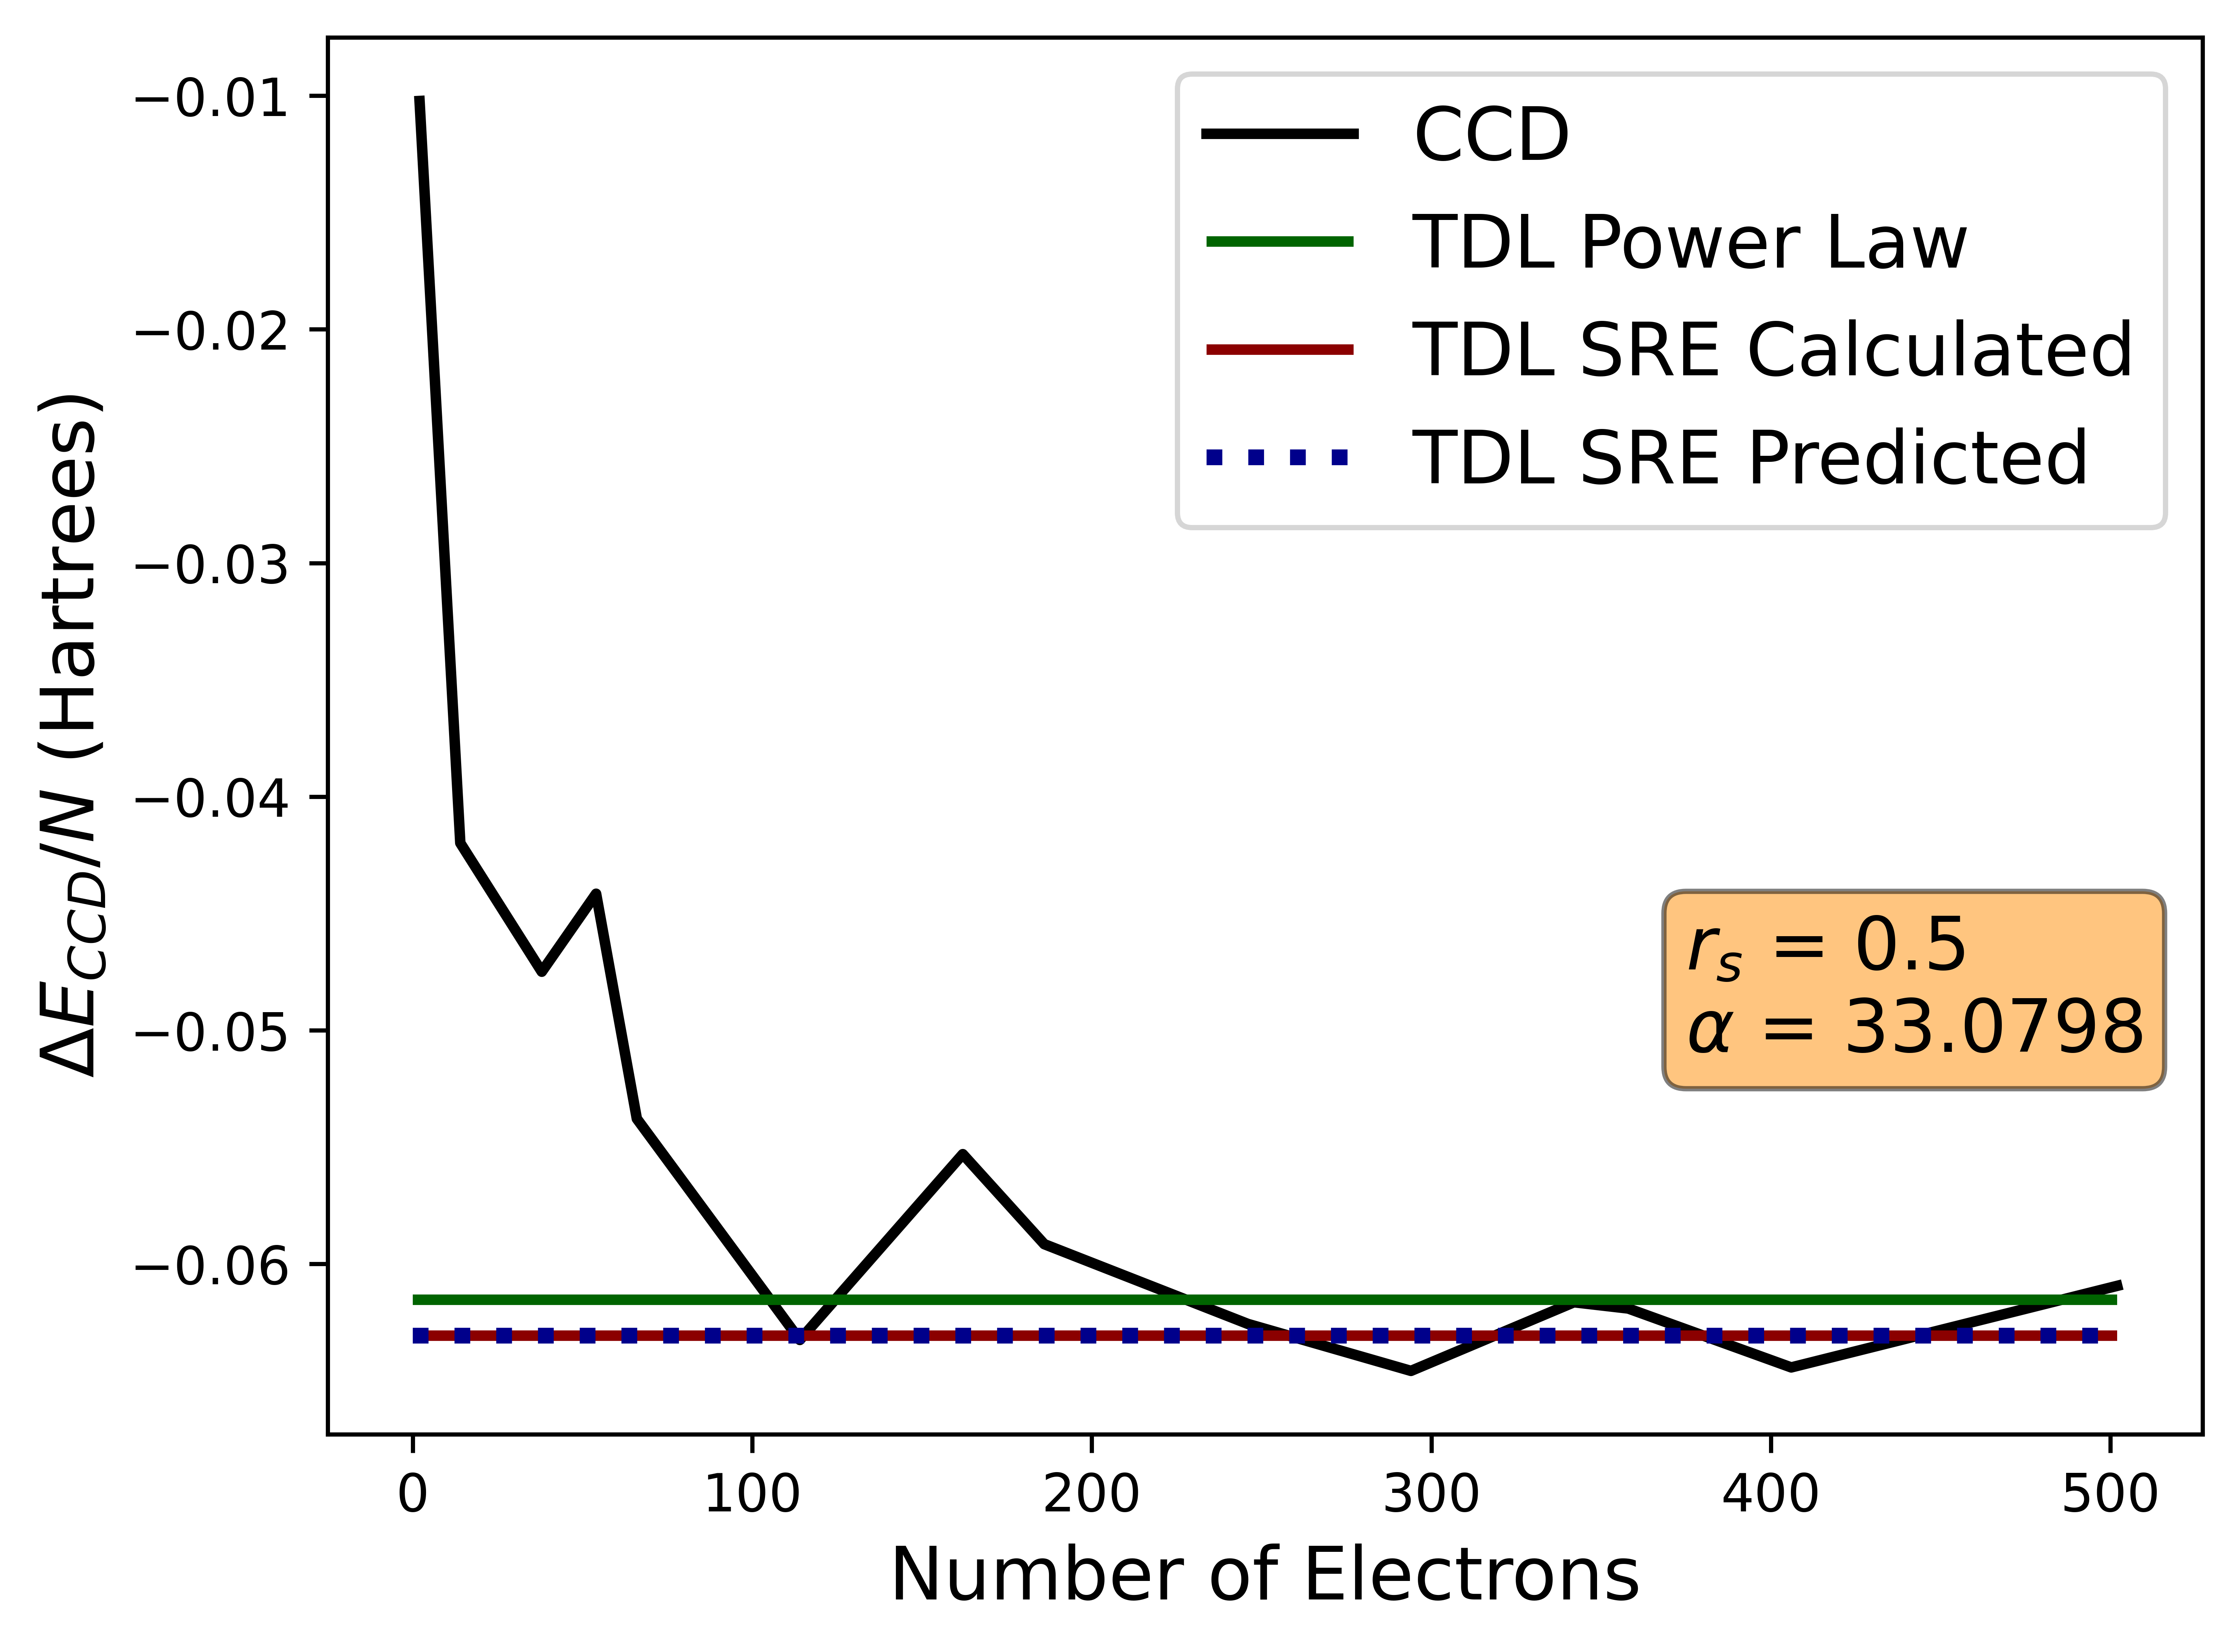
\includegraphics[scale=0.5]{Images/Chapter7/TDL_0.5.png}
    \caption{The CCD correlation energy per electron for an HEG with $r_s$ = 0.5 and calculated at M = 6,142 (black).  The power law prediction for the TDL correlation energy per electron is shown in green, and the SRE predictions for the TDL correlation energy per electron extrapolated from calculated and predicted energies are shown in red and blue, respectively.}
    \label{fig:TDL_0_5}
\end{figure}

%%% THESIS CONCLUSIONS %%%

% SRE as a valid extrapolation method
The sequential regression extrapolation (SRE) method developed here based on Bayesian regression algorithms is an accurate and valuable extrapolator for removing basis incompleteness errors from coupled cluster calculations of infinite matter systems. Furthermore, when the infinite matter system needs to be taken to the thermodynamic limit, it is possible to use SRE to perform this task. Since the SRE algorithm uses training data taken from calculations at small numbers of single-particle states to predict the correlation energy at many single-particle states, the SRE algorithm can offer significant time savings over performing fully converged correlation energy calculations. As shown in this thesis, using the SRE algorithm to save over 100 node hours in the calculations of just one correlation energy is possible. Furthermore, this huge time savings does come with a loss in the accuracy of performing the whole savings. However, the average percent error between the SRE prediction and the fully calculated result was typically less than 1$\%$, making it quite a slight difference compared to the large amount of computational time that has been saved.

% From the CCD vs. CCDT side
Furthermore, besides developing the SRE method, we also compared different methods of performing coupled cluster calculations of systems of infinite nuclear matter. First, we compared the results from two different interactions: the Minnesota potential, a toy interaction, and chiral NNLO potentials, which are much more realistic. By comparing these two, we learned that they differ quite significantly around densities of infinite nuclear matter that are similar to nuclear densities and that calculations containing NNLO potentials do take much longer to compute compared to a Minnesota potential applied to the same system. Furthermore, we could also compare the difference between the coupled cluster approximations CCD, CCDT-1, and CCD(T) on calculations of infinite matter systems. We found that the triples approximations give significant results when compared to the CCD approximation, so they are worth performing even though they provide an increase in computational time.

%% SIZE OF MACHINE LEARNING SYSTEM
Though it has been mentioned throughout this thesis, it is essential to emphasize the size of the training data sets used in this work. This work's most extensive training data set used only 16 training points, and the smallest training set used only 3 points. Some areas of physics could be faster to adopt machine learning because of the vast amount of training data that some machine learning algorithms require. However, this work has shown that accurate machine learning predictions can be made with very few training points, thus encouraging using machine learning as a tool in fields with small data sets.

%%% FUTURE WORKS %%%

\subsection*{Possible Future Works}
% Full triples and different proton fractions
A few notable future works stem directly from the work presented here. First, while we showed results from both the CCD< CCDT-1, and CCD(T) approximations, we did not have the capabilities to produce coupled cluster correlation energies using a complete CCDT calculation. This is mainly due to the high computational costs of a complete triple calculation ($O(M^8)$), but advancements, such as those made in Refs. Furthermore, ADD REFERENCES HERE are making this a much more achievable goal for the near future.

Additionally, while we only looked at pure neutron matter and symmetric nuclear matter here, there are other proton fractions of interest. If we want to model the equation of the state of nuclear matter thoroughly, then we need to be able to accurately predict the properties of neutron matter at proton fractions beyond just 0.0 and 0.5.

% PARAGRAPH ABOUT NOT BEING LIMITED TO INFINITE SYSTEMS
While truncating the number of particles in a calculation is limited to infinite matter and other large systems, truncations occur in every \textit{ab initio} many-body calculation. Basis truncation is especially common and occurs in almost every calculation except some simple toy models. The last part of this thesis will be dedicated to exploring some possible future applications of the SRE methodology which has been developed.

% PARAGRAPH ABOUT CC CALCULATIONS OF THE NUCLEUS
An extension of the work presented in this thesis is to apply the SRE method to remove basis incompleteness errors from coupled cluster calculations of nuclei. Though nuclei are finite systems and the number of nucleons in the system generally does not need to be truncated, the number of single-particle states is still truncated, leading to a need to extrapolate to an infinite model space \cite{Ref6}. This is especially true for heavy nuclei and nuclei that are weakly bound \cite{Ref6}. There are methods to perform these extrapolations on nuclei calculations, but when using the harmonic oscillator basis, which mixes the ultraviolet and infrared cutoffs, these extrapolation methods can fail \cite{Ref6}. Machine learning has been used to perform similar extrapolations (see Ref. \cite{Ref6}, \cite{Ref22}, \cite{Ref23}, for example), but these were performed with neural networks and thus incurred all of the problems that were experienced with neural networks in this thesis.

%% MBPT CALCULATIONS AND HIGHER ORDERS
Additionally, the SRE method has no reason to be restricted to only predicting CC energies using MBPT2 energies. Extending the SRE method to other many-body methods should also be possible. 

% PARAGRAPH ABOUT FCI
One of the most accurate yet restricted \textit{ab initio} many-body methods is full configuration interaction theory (FCI), which uses a variationally optimized linear combination of the full set of Slater determinants. FCI is used in nuclear physics and electronic-structure theory, but its complexity limits it to only the smallest of systems. The ground state energy, which FCI finds, is the lowest (variationally) and most accurate that can be achieved. If an infinite single particle basis is used, FCI produces the solutions to the Schr\"{o}dinger equation. However, due to computational limitations, FCI calculations must be performed with a finite basis, meaning they will fail to retrieve the total energy \cite{Ref1}. However, it is possible that SRE could be applied to FCI calculations using, for example, Hartree Fock calculations as the "fast method" to quickly and accurately extrapolate FCI results to the infinite basis limit, thus recovering the Schr\"{o}dinger equation results.

 % APPLICATIONS OUTSIDE OF NUCLEAR PHYSICS
While most of this thesis, except for the sections on the electron gas, have been devoted to nuclear physics applications, \textit{ab initio} many-body methods occur in many other fields besides nuclear physics. For example, coupled cluster theory, and other many-body methods, are prevalent in other fields of physics and quantum chemistry. Therefore, the development of the SRE method should improve calculations outside of the realm in which it was developed.

%%%%%%%%%%%%%%%%%%%%%%%%%%%%%%
%% CHAPTER: INFINITE NUCLEAR MATTER RESULTS
%%%%%%%%%%%%%%%%%%%%%%%%%%%%%%
\chapter{Infinite Nuclear Matter Results}
    %% ADD SOMEH+THING HERE ABOUT USING ELECTRON GAS AS A TEST BED TO DEVELOP METHODS BUT NOW ARE GOING TO FOCUS ON GPs AND APPLY IT TO 


We have explored and developed the SRE method by applying it in various ways to the infinite electron gas.  The electron gas, with its shorter computational times and more straightforward interactions, makes it an excellent test bed to develop methods that can be applied to other infinite matter systems. This chapter studies one of these more complicated systems: infinite nuclear matter.  Therefore, we will be using SRE methods perfected on the electron gas. For this chapter, all SRE algorithms use Gaussian processes with a modified rational quadratic kernel that was developed in the last section of the previous chapter.  We will start our studies in this chapter with pure neutron matter with both toy and realistic nuclear interactions and then move on to symmetric nuclear matter with realistic interactions before concluding with a brief study of the symmetry energy of infinite nuclear matter.
    %%%%%%%%%%%%%%%%%%%%%%%%%%%%%%
    %% Pure Neutron Matter
    %%%%%%%%%%%%%%%%%%%%%%%%%%%%%%
    \section{Pure Neutron Matter}

        \subsection*{Coupled Cluster Doubles and the Minnesota Potential}
As a toy nuclear interaction, the Minnesota potential will provide us with approximations to the energies for a pure neutron matter system, but without a high degree of accuracy. However, the Minnesota potential is less computationally taxing than the more realistic chiral potentials and only includes two-body forces; the Minnesota potential, like the HEG, is a valuable test bed for further developing our SRE method before we apply it to the more realistic nuclear matter calculations with the chiral potentials.

\subsubsection*{Gaussian Processes}
The training data for each combination of density and the number of neutrons was taken to be the CCD and MBPT2 correlation energies between 5 open energy shells and 14 open energy shells (inclusive). This data was formatted using the process described in Chapter 6. The machine learning algorithm used to analyze these data sets was Gaussian Process (GP). For each data set, the alpha value of the GP algorithm was set to be the standard deviation of the training data set. The kernel for the GP algorithm was chosen to be a white kernel multiplied by a rational quadratic kernel, added to a white kernel (all kernels are Scikit-Learn's implementation). The hyperparameters of the kernels were set by the GP algorithm during the training process. Once each GP was trained, it was asked to predict 100 data points, leading to a converged ratio of correlation energies. The final point in this data set was taken to be m and was multiplied by $\Delta E_{MBPT,6142}$ to give an approximation for $\Delta E_{CC,6142}$. Additionally, the GP algorithms produced their uncertainties on all of the plotted predictions and the results in Figure \label{pnm_mp_all}.

\begin{center}
    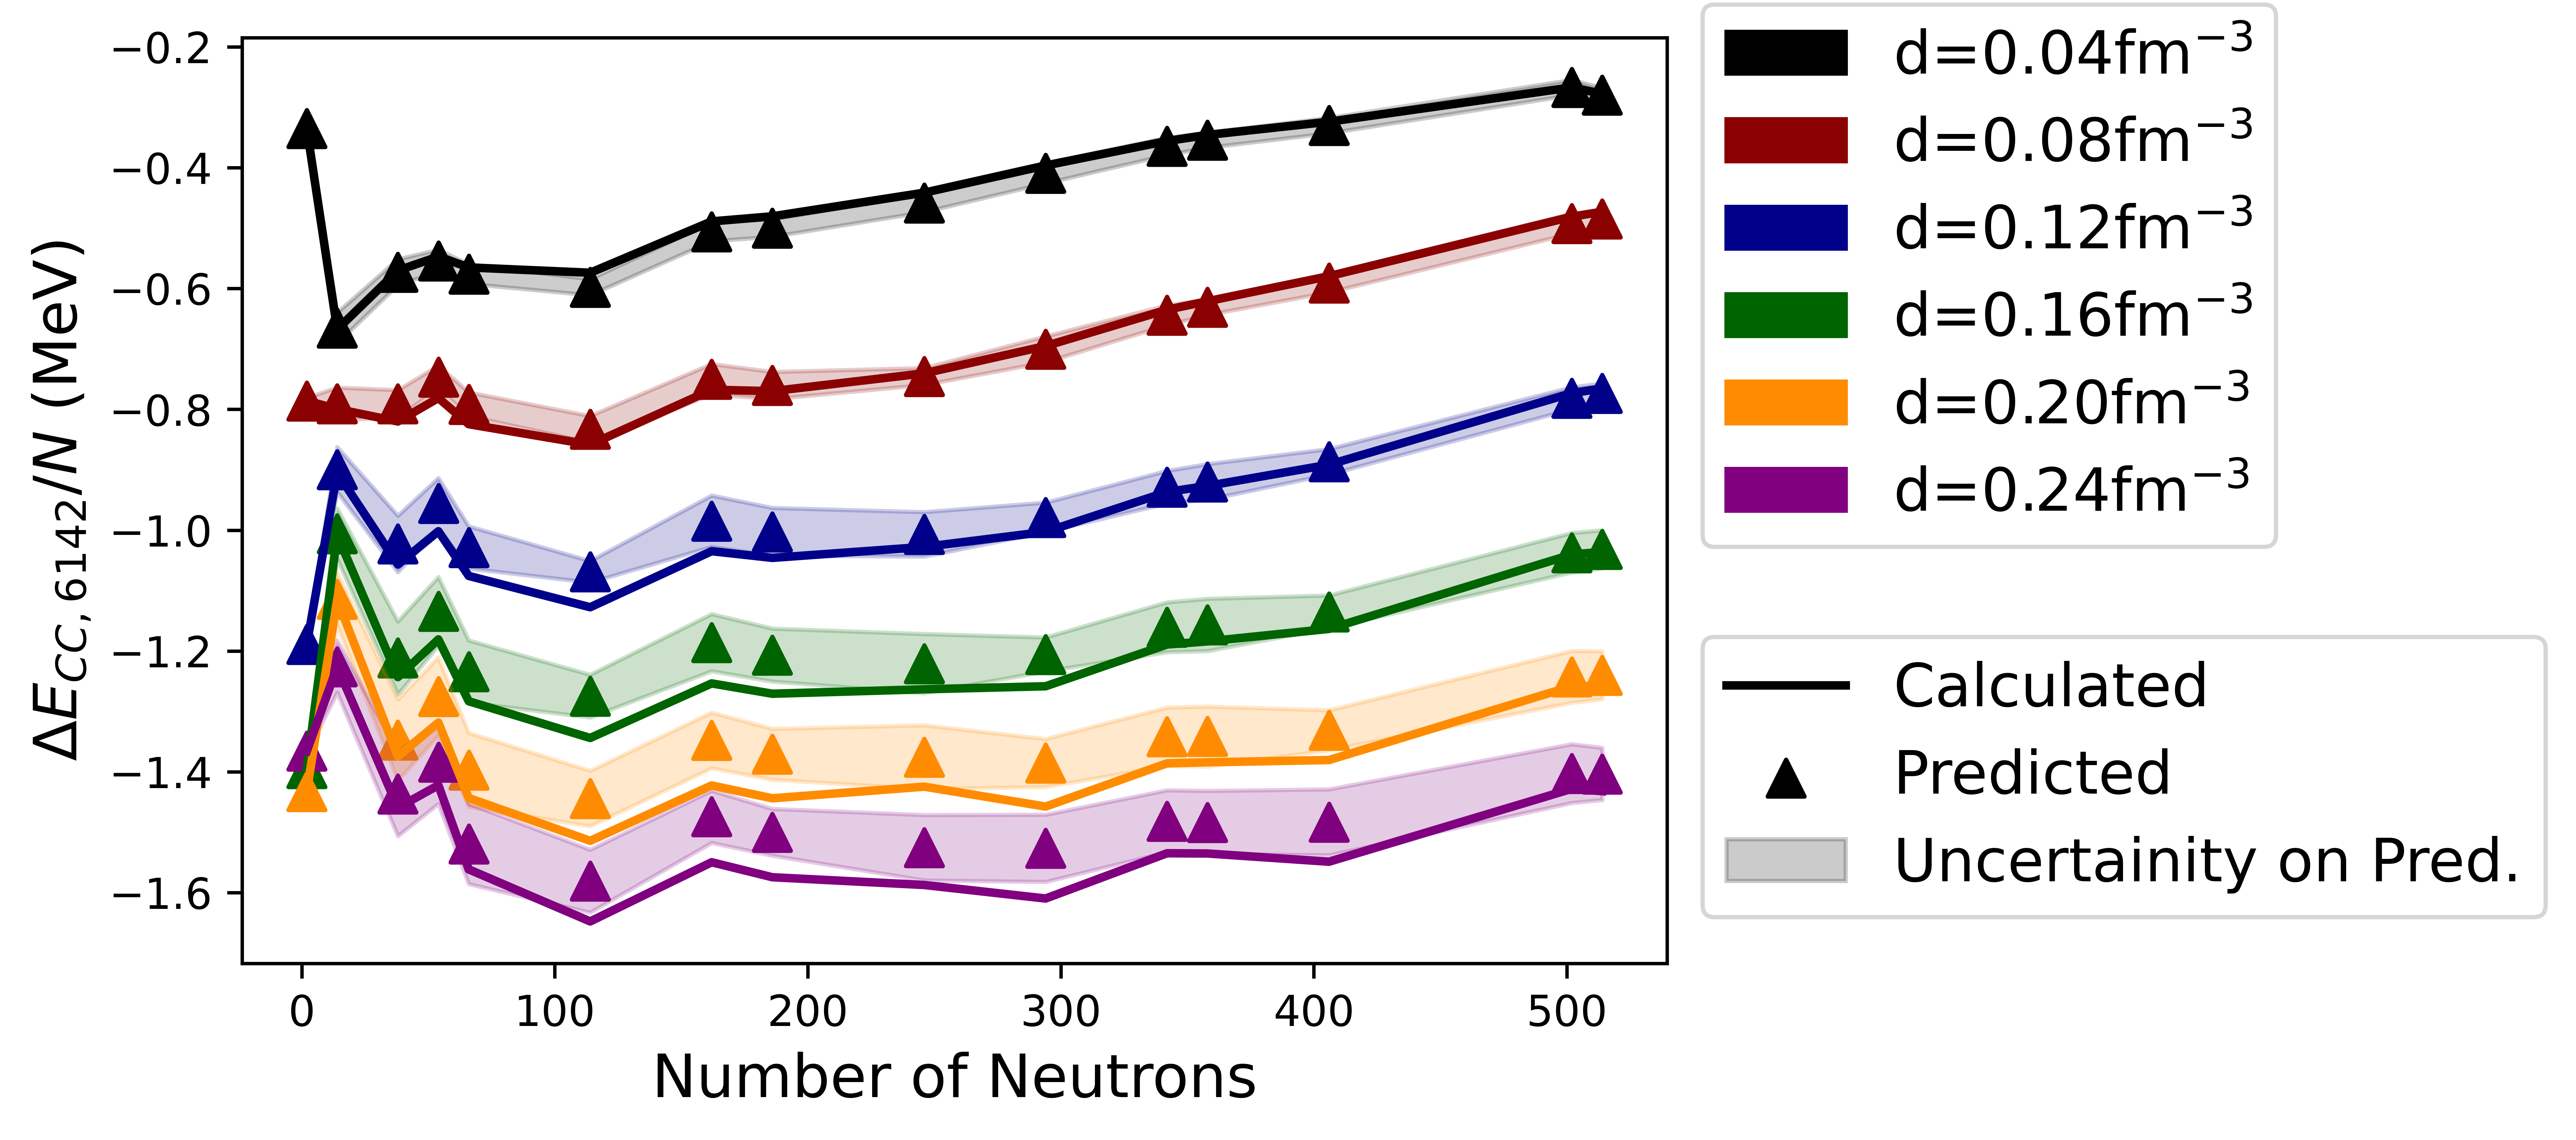
\includegraphics[scale=0.75]{Images/Chapter7/NeutronMatter/GP_PNM_MSU_n_1_uncertainity.png}
    \captionof{figure}{The CCD correlation energy per neutron as a function of the number of neutrons in the system for pure neutron matter with the Minnesota potential. All calculations are performed at 6,142 single particle states and with periodic boundary conditions. The full calculations, shown with the solid lines, were performed on MSU's ICER supercomputer. The SRE predictions, shown with the triangular data points, were predicted using only ten training data points from 5-14 open shells. The shaded region shows the Gaussian process uncertainty in predicting the converged correlation energy per neutron. The overall RMSE error between the full calculated and the predicted CCD correlation energies per neutron is 0.037 MeV.}
    \label{pnm_mp_all}
\end{center}

When looking at these results, it is also essential to consider the errors associated with other approximation schemes that do not involve machine learning—truncating the number of single-particle states in the system to some set number of energy shells. For example, if we limit the calculation to 14 open energy shells (15 to 30 shells), the error from the CCD correlation energies at 70 shells (M = 6,142) is 0.56 MeV, much larger than the GP result of 0.037 MeV. Furthermore, we can place include more energy shells before truncating. For example, if 40 total shells are included in the calculation, then the RMSE error from the results at 70 shells is 0.26 MeV; for truncating at 50 total shells, it is 0.15 MeV, and for truncating at 65 total shells, it is 0.045 MeV.  Therefore, even when exerting significant computational time and resources to raise the truncation level of the calculations, the GP prediction made with very little training data collected at a low number of energy shells is still the most accurate.

Accuracy is not the only metric we must consider; we must also consider the computational time and resources needed to generate the training data and perform the ML analysis versus just performing the complete calculation. The timing data presented in this paragraph was collected on Michigan State University's HPCC supercomputer on Intel Xeon processors with 2.40 GHz and 240 GB of RAM. The coupled cluster code was memory-optimized using the diagonal block structure developed in Ref. \cite{Ref5} and was parallelized using four compute nodes and 28 threads per node. Fig. \ref{pnm_mp_all} contains 90 points, each of which has to be individually calculated or predicted with the machine learning algorithm. Since each machine learning process has 15 points, 1,350 training points are needed to produce Fig. \ref{pnm_mp_all}.  However, their run times are comparatively short since they are from 5-14 open energy shells. Generating all 1,350 training data points takes 34.12 hours. It takes about 20 seconds to perform all 90 ML analyses, thus adding a negligible amount of time to the total ML analysis run time, which will be dominated by the time to generate the training data. To generate all 90 data points in Fig. \ref{pnm_mp_all} at 70 energy shells each, the total run time is 121.74 hours, meaning that by using the ML extrapolation method instead, 87.61 hours of computational run time is saved. That is equivalent to over 3.5 days of computational time saved and a resulting error of only 0.037 MeV!

It is possible to achieve better accuracy with this prediction method by changing the alpha hyperparameter of the Gaussian process algorithm. Instead of using the standard deviation of the training data as the alpha parameter (as used to generate Fig. \ref{pnm_mp_all}), instead we will use the fourth root of the standard deviation of the training data ($\alpha = \delta y_{train}^{1/4}$). However, while doing this increases the accuracy (the RMSE drops from 0.37 MeV to 0.25 MeV), the uncertainty drastically increases. As mentioned earlier, when working with these Bayesian algorithms, there seems to be a trade-off between the accuracy of the predictions and the size of the standard deviation of the prediction. The results for performing this extrapolation are shown in Fig. \ref{pnm_mp_all_n_0_25}, where the uncertainties are shown in (a) but are removed in (b) for clarity.

\begin{figure}[H]
\centering
\begin{subfigure}{0.48\textwidth}%
  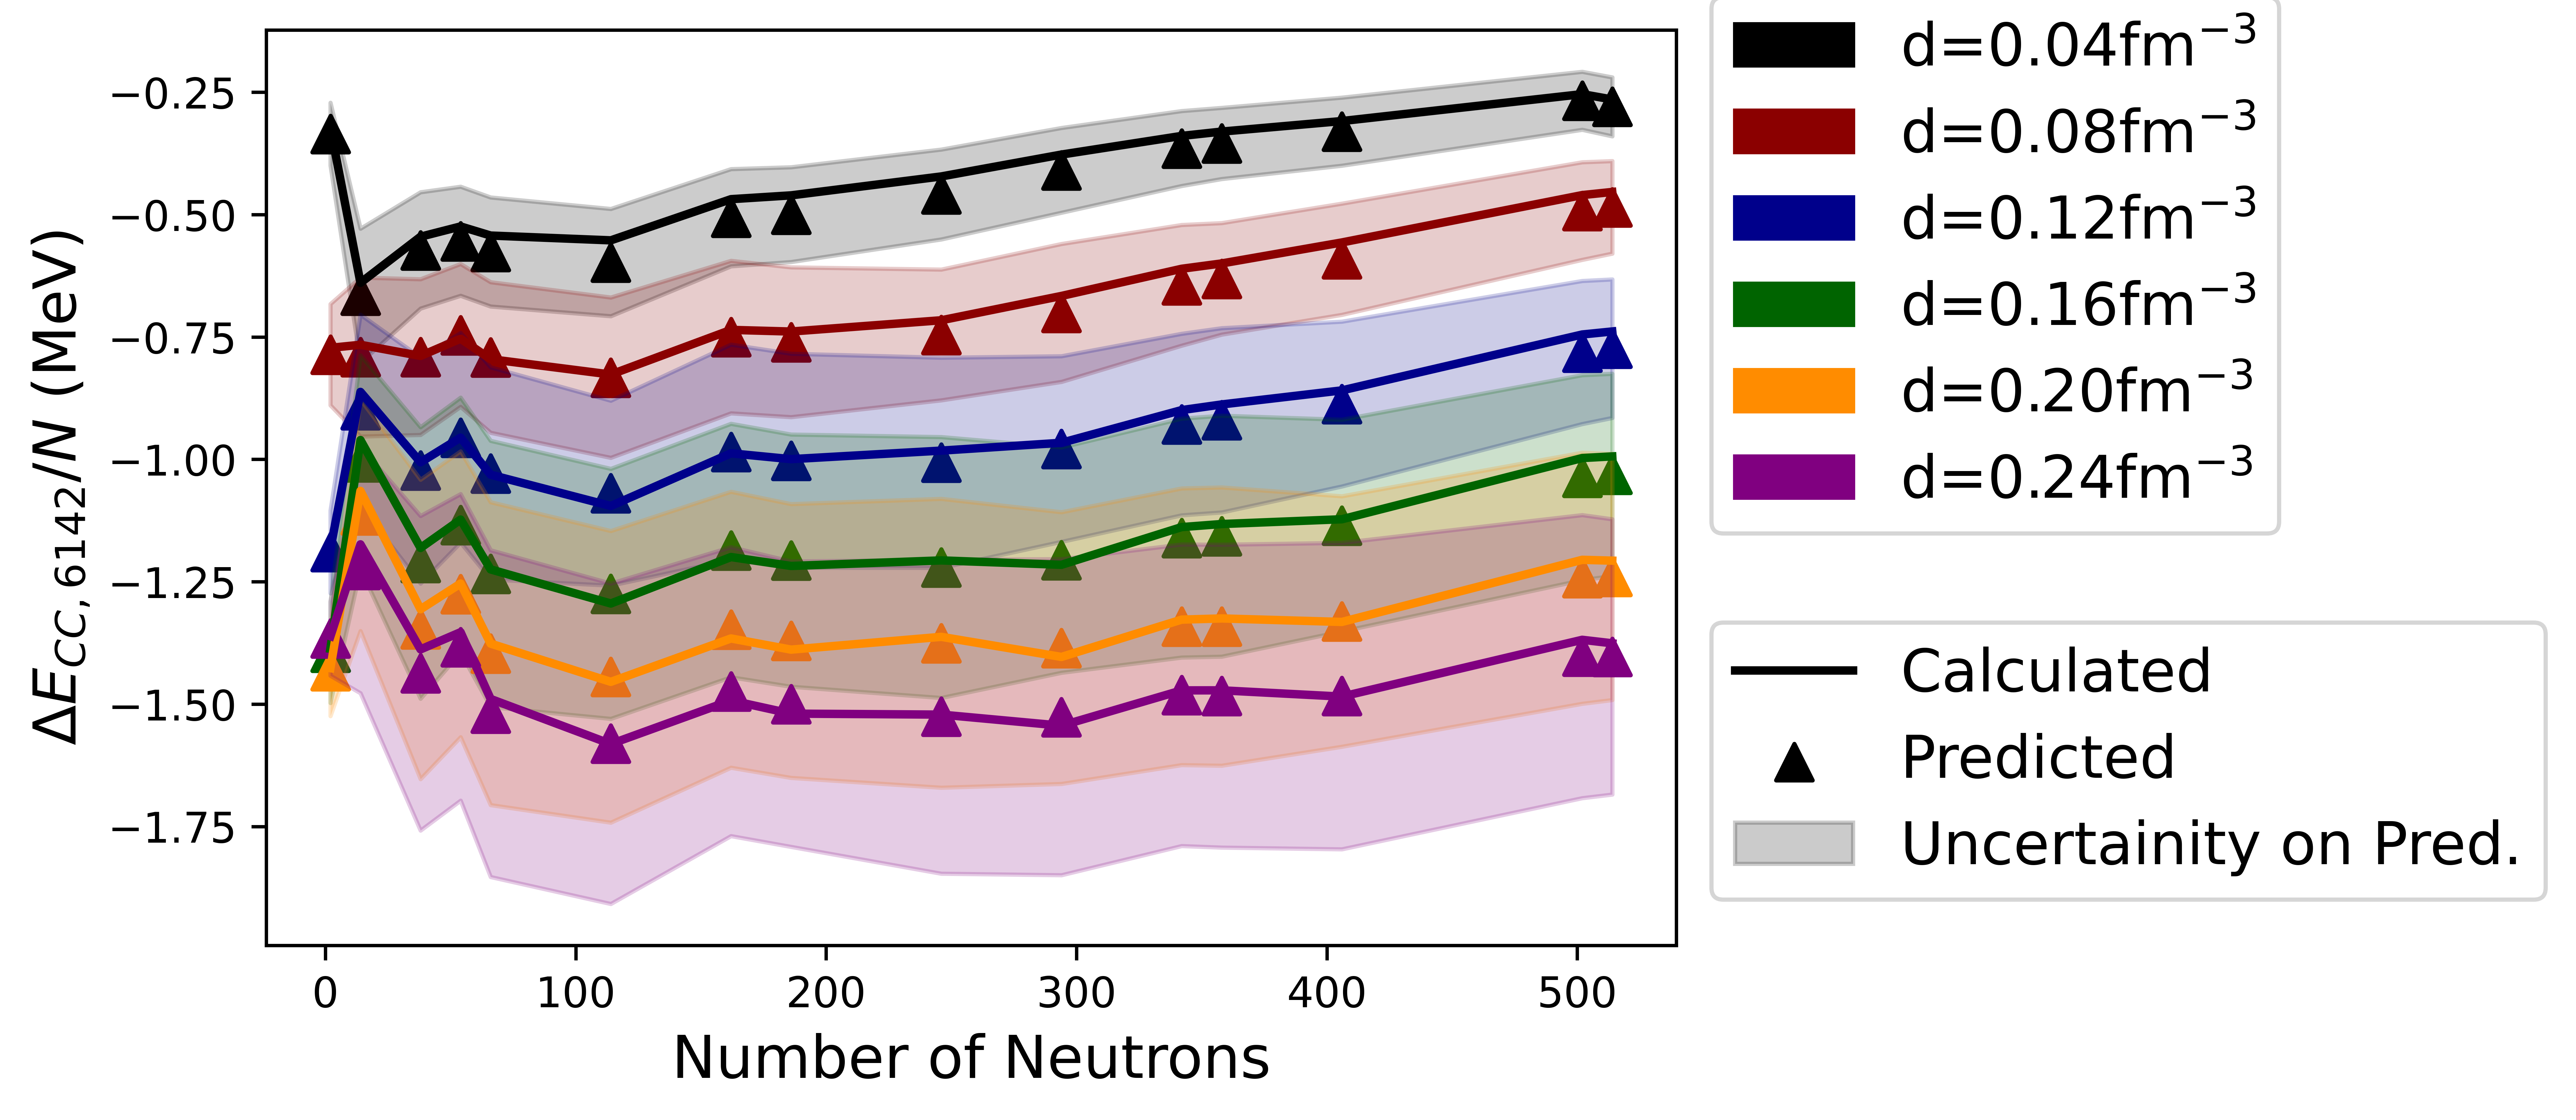
\includegraphics[width=\textwidth]{Images/Chapter7/NeutronMatter/GP_PNM_MSU_n_0_25_uncertainity.png}%
  \caption{A subfigure}
  \label{fig:sub1}
\end{subfigure}~%
\begin{subfigure}{0.48\textwidth}%
  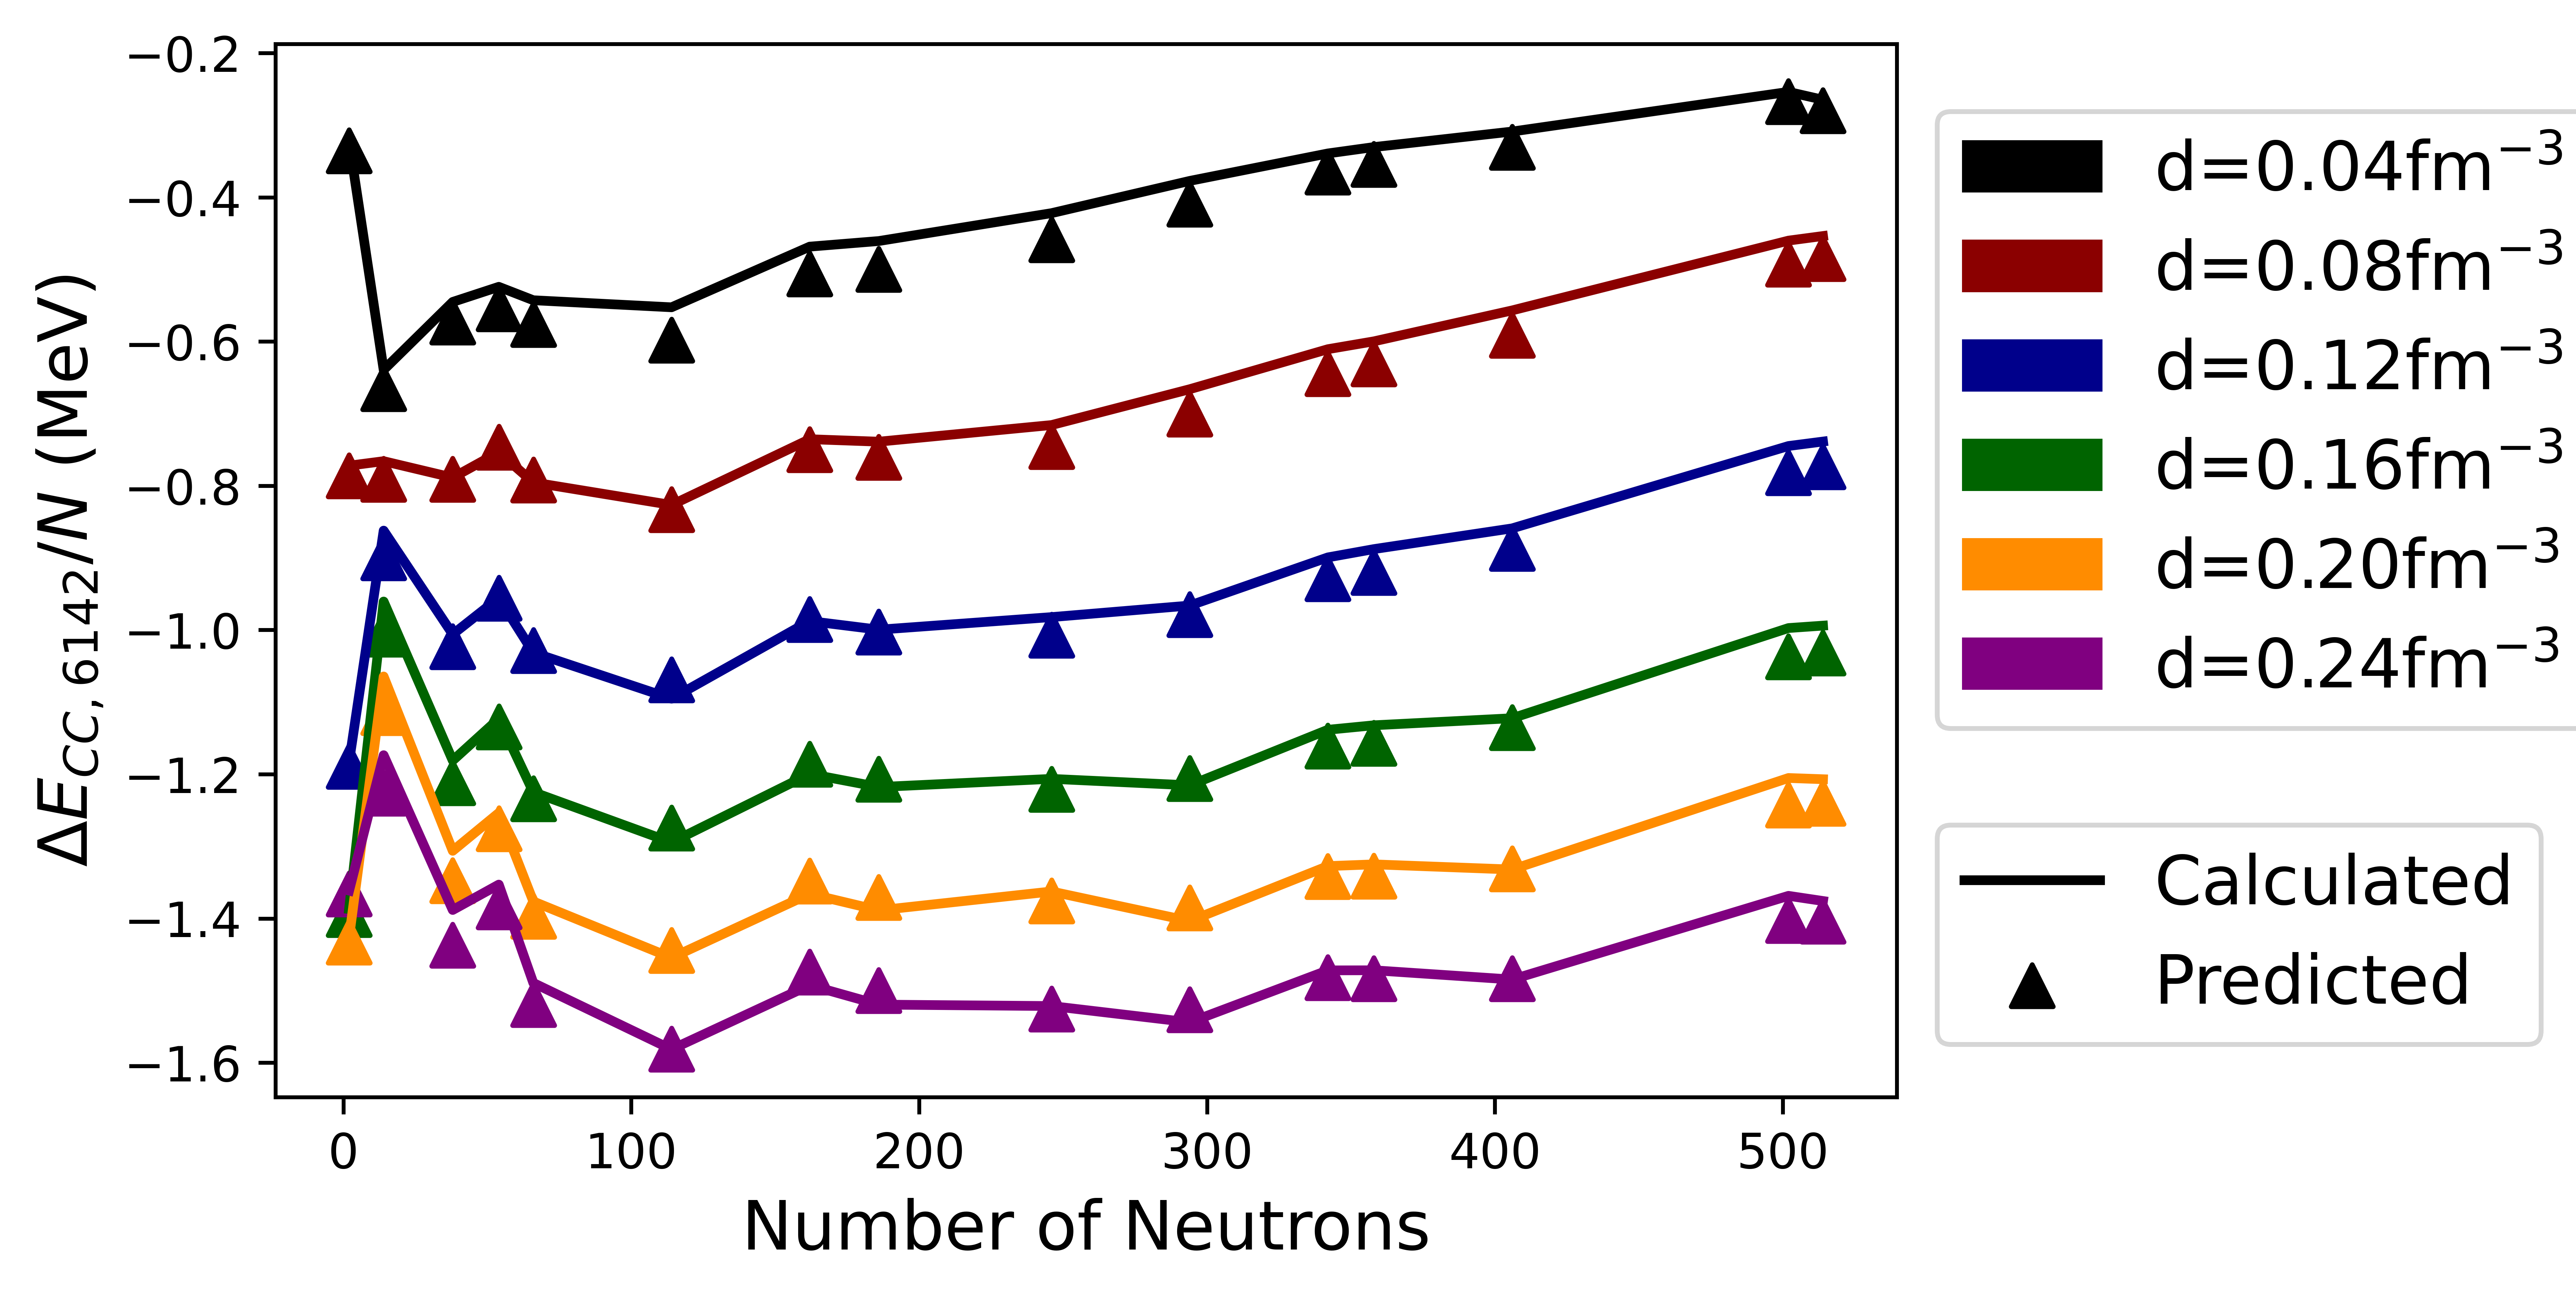
\includegraphics[width=\textwidth]{Images/Chapter7/NeutronMatter/GP_PNM_MSU_n_0_25.png}%
  \caption{Another subfigure}
  \label{fig:sub2}
\end{subfigure}
\caption{A figure with two subfigures}
\label{pnm_mp_all_n_0_25}
\end{figure}
        \subsection*{Coupled Cluster Doubles and Realistic Potentials}

In this section, we will perform CCD correlation energy calculations on a pure neutron matter system, using chiral potentials derived from effective field theory (EFT) to model the nuclear interaction. These potential more realistically models the nuclear interaction when compared to the Minnesota potential, so these results are expected to be more accurate than the Minnesota potential results from the previous section. Specifically, we use next-to-next-to-leading order (NNLO) chiral potentials in this section.

We will limit our calculations to a 66 neutron system for the chiral potential. This is done for two reasons. Ref. \cite{Ref8} and \cite{Ref9} show that, especially for pure neutron matter, calculations for a system of 66 neutrons are nearly indistinguishable from calculations performed at the infinite matter limit. So for 66 neutrons, the finite size error in a pure neutron matter calculation is minimized. Therefore, we do not need to perform extrapolations at higher values of N to perform an N$=\longrightarrow$ $\infty$ extrapolation.

Secondly, the CCD correlation energy calculations for pure neutron matter with chiral potential are very time intensive, much more so than pure neutron matter calculations with the Minnesota potential. For the Minnesota potential, the average time to generate converged CCD correlation energies across all densities in Figure \ref{pnm_mp_all} for 66 neutrons is 5.87 minutes. These calculations were all performed at 70 total energy shells or 6,142 single-particle states. However, when we perform the same calculations with the realistic chiral potentials from EFT, the average run time across all densities shown in Figure \ref{fig:ornl_pnm_ccd} is 2.32 hours per calculation. Moreover, these calculations converge at a much lower number of single-particle states, so these calculations were performed at 1,478 single-particle states or 27 total energy shells. Note that these calculations were performed with different codes, written in different languages, and performed with different high-performance computing set-ups. Hence, the run times are not directly comparable. However, it is sufficient to say that performing these calculations with realistic chiral potentials is much more computationally challenging than using the Minnesota potential.

As a further motivation for applying the SRE method to this system, let us examine the computational time and resources needed to perform calculations on a pure neutron matter system with 66 neutrons, a density of 0.16 fm$^{-3}$, and chiral NNLO potentials. Fig. \ref{fig:nnlo_ccd_times} shows the computational time in node seconds needed to perform the CCD correlation energy calculations as the number of single-particle states increases.

\begin{figure}
    \centering
    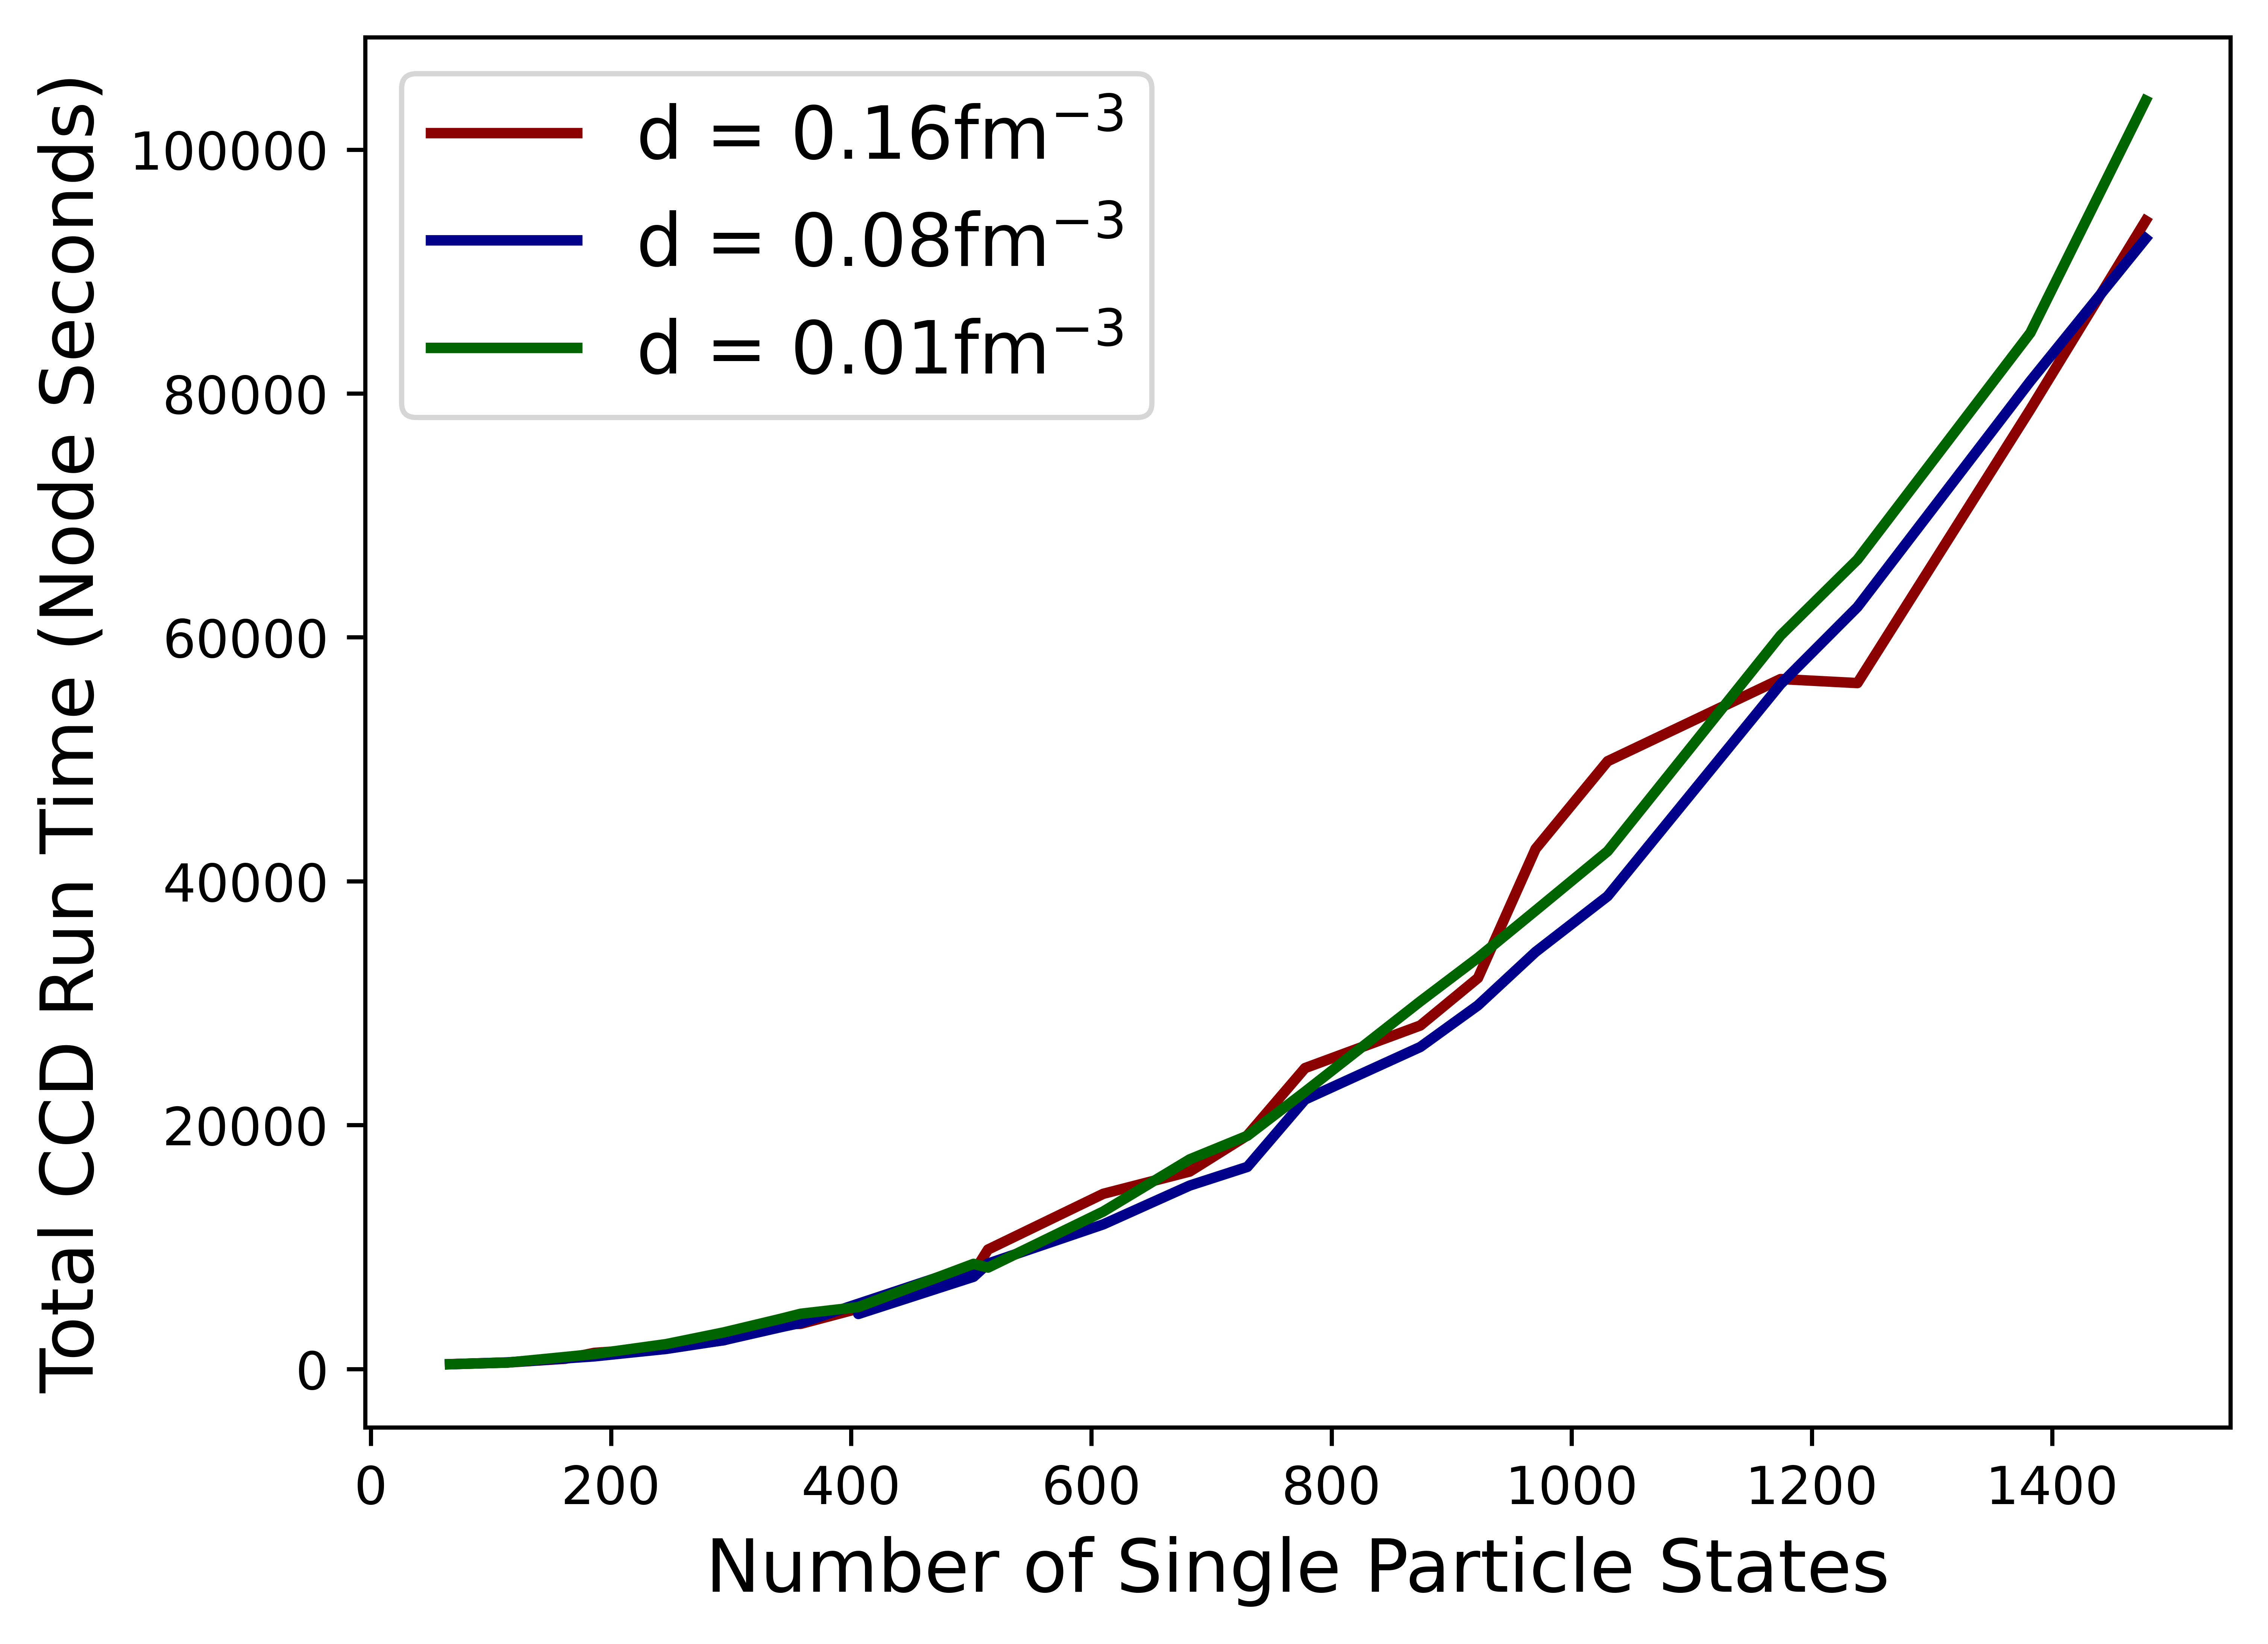
\includegraphics{Images/Chapter7/ORNL/pnm_times.png}
    \caption{Caption}
    \label{fig:nnlo_ccd_times}
\end{figure}


Figure \ref{fig:ornl_pnm_ccd} shows CCD calculations and ML predictions for pure neutron matter at 66 neutrons at two different density ranges. Figure \ref{fig:pnm_ccd_nuclear} shows a density range around nuclear density (which nuclear density being $\approx$ 0.16 fm$^{-3}$), and Figure \ref{fig:ornl_pnm_ccd_low} shows a low-density range. Densities around nuclear density are essential for studies of nuclei. The outer layers of a neutron star are thought to have densities around nuclear density (\cite{Ref3} \cite{Ref9} \cite{Ref16}), while the matter at the center of a neutron star is thought to be a low density (CITATION NEEDED). The ML specifications for the plots in Figure \ref{fig:ornl_pnm_ccd} are as follows. For \ref{fig:pnm_ccd_nuclear}, each ML prediction was made using only three training data points, MBPT2 and CCD correlation energy calculations between 114 and 186 single-particle states (or between 1 and 3 open shells). We were able to use such a small number of training points here because the correlation energies converge rather quickly. The SRE sequence length was chosen to be one here since there are only three training points. The converged CCD calculations in the figure were calculated at M=1,478 single particle states or 27 total energy shells (22 open energy shells). This number of single-particle states was chosen as the converged values because it is similar to the number of single-particle states used to calculate converged values in similar studies (Refs. \cite{Ref8}, \cite{Ref9}, and \cite{Ref20}). The same Gaussian Process algorithm and kernel as the Minnesota potential analysis was also used here, but the variance of the algorithm was chosen to be the standard deviation of the training data to the fourth power ($\alpha = \delta y_{train}^{4}$). For Figure \ref{fig:ornl_pnm_ccd_low}, the GP specifications are the same, but for the training data, seven training points were used from 186 to 502 single-particle states (3 to 9 open energy shells). This change was made because the correlation energy converges slower at lower densities. The SRE sequence length was also increased to three since more training data is available. The CCD correlation energy at M = 1,478 was still used at the fully converged value, though, and its convergence was confirmed.

\begin{figure}
\centering
\begin{subfigure}{.45\linewidth}
  \centering
  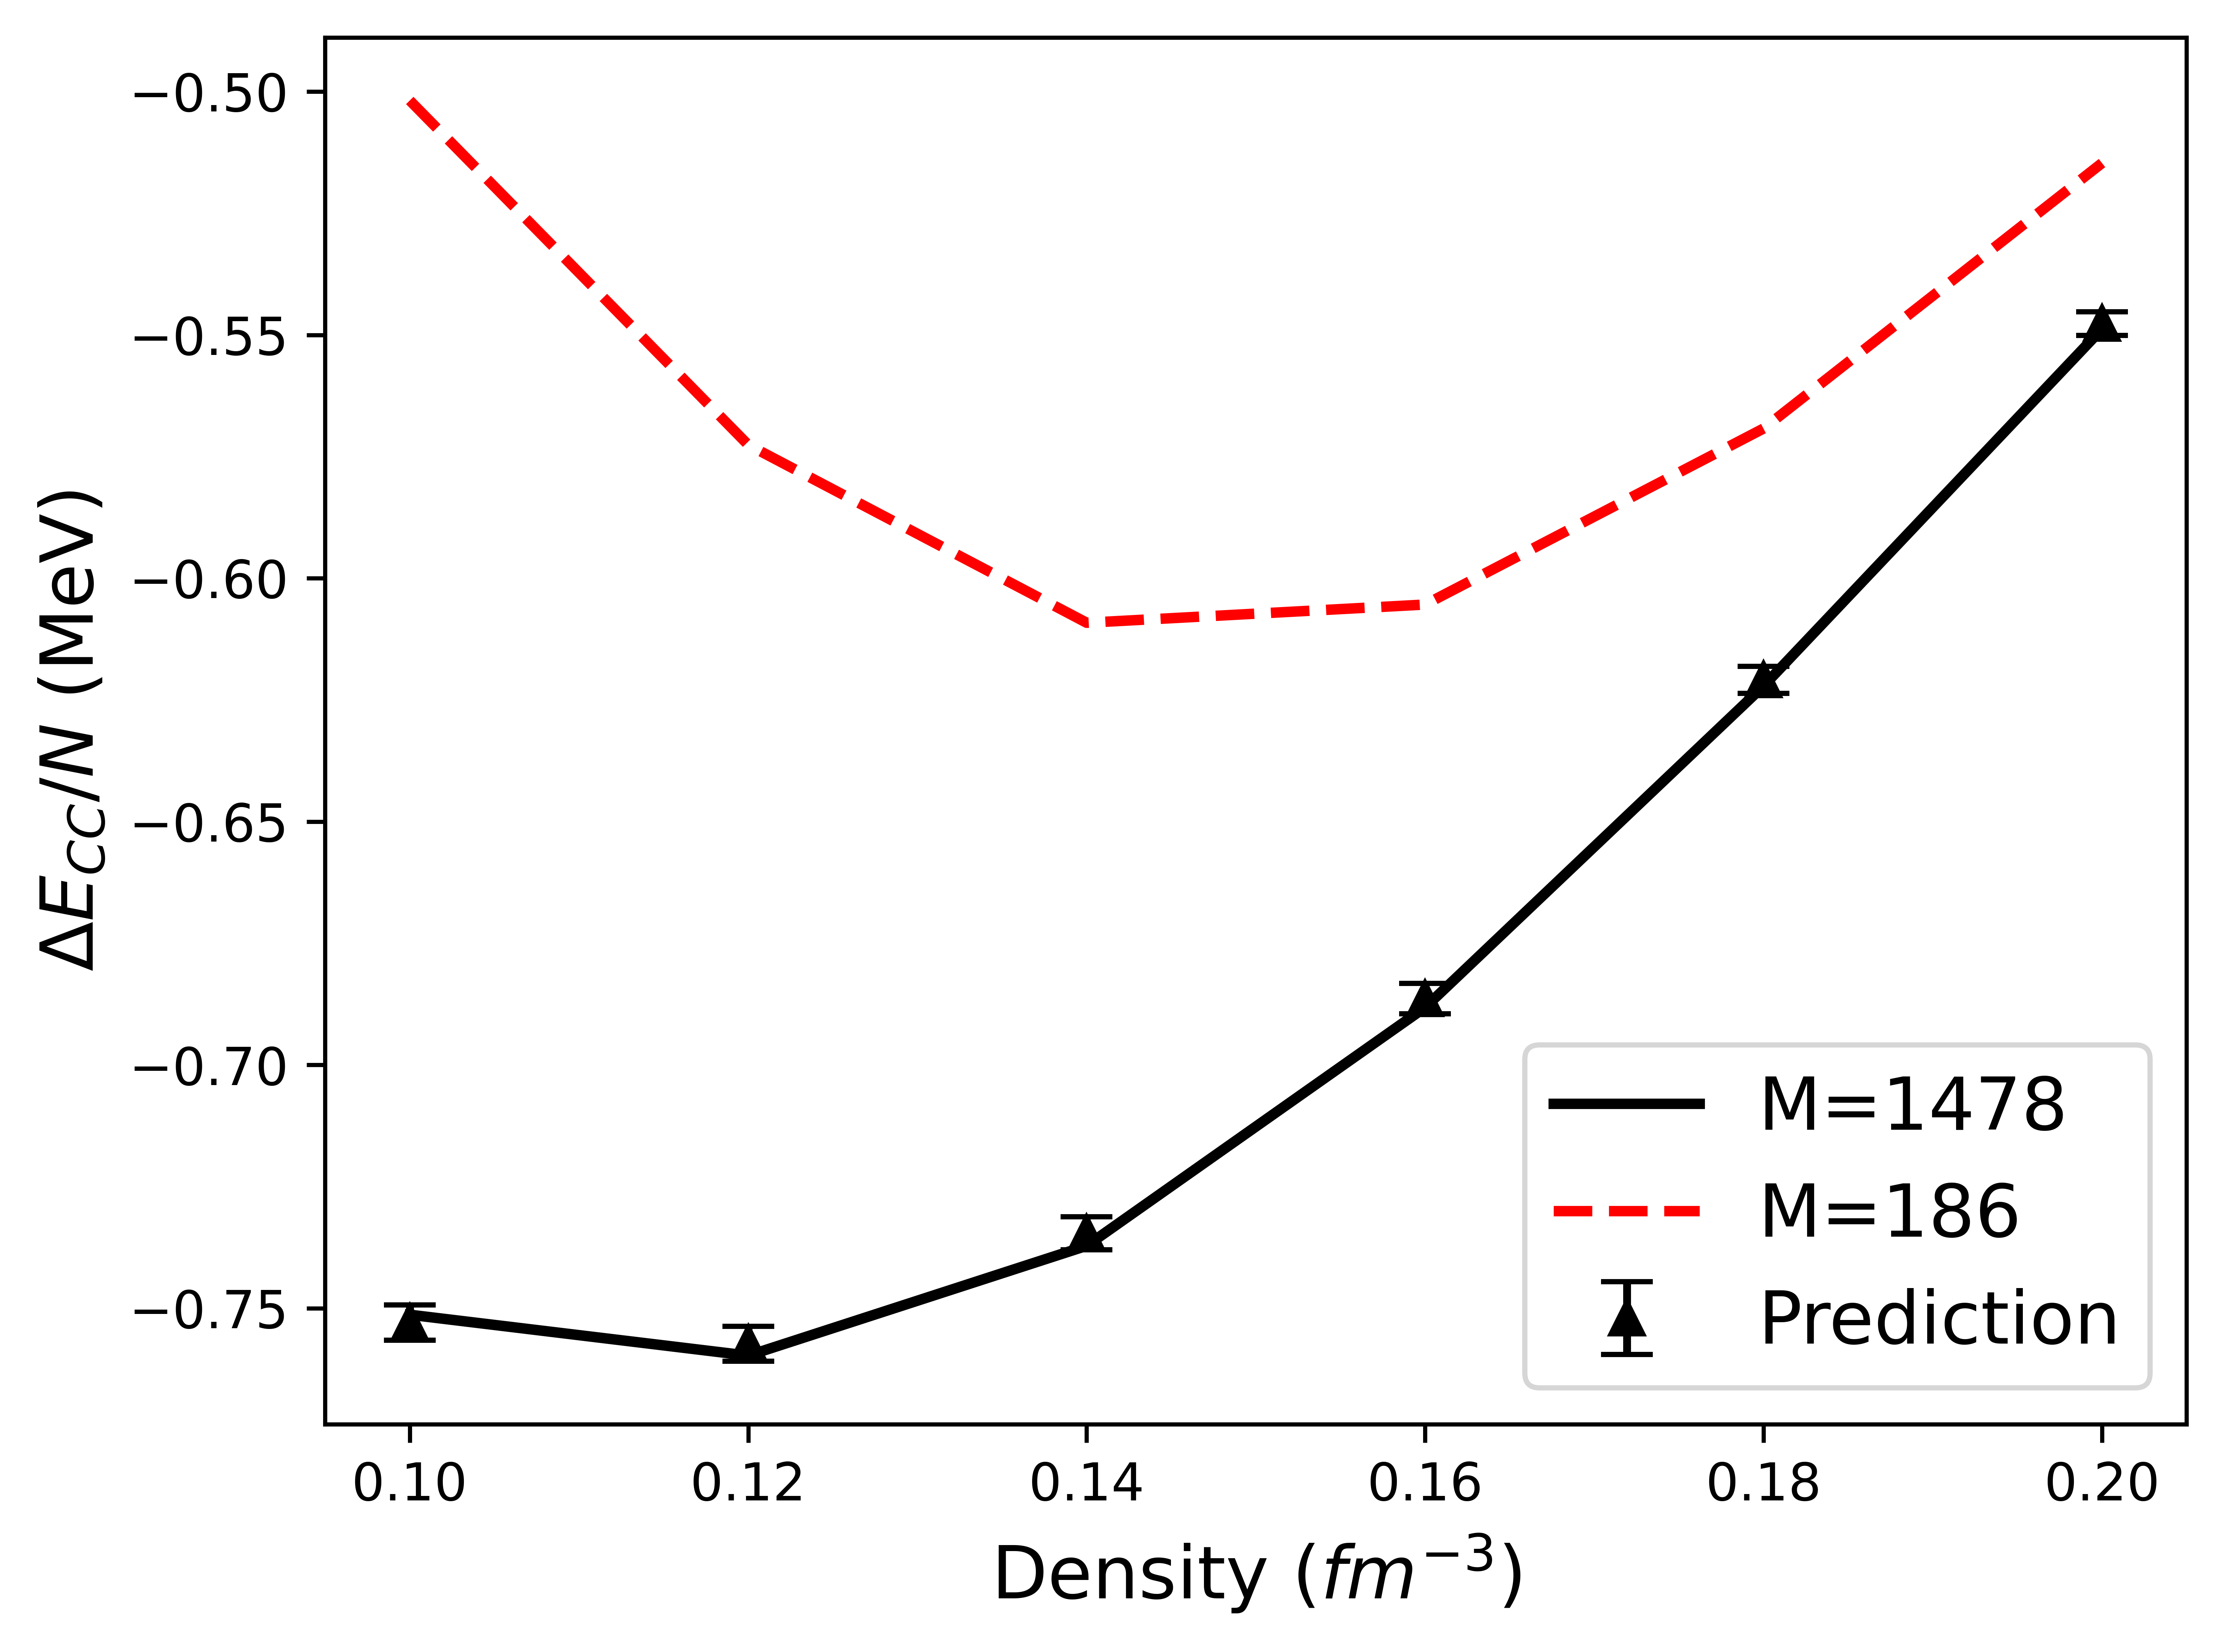
\includegraphics[scale=0.5]{Images/Chapter7/ORNL/neutron_matter-4.png}
  \caption{The results from predicting the converged $\Delta E_{CCD}/N$ for pure neutron matter at densities around nuclear density.  The average percent error across all densities is 0.25$\%$, and the time savings from generating only the training data versus the fully converged $\Delta E_{CCD}/N$ is 12.71 hours.}
  \label{fig:pnm_ccd_nuclear}
\end{subfigure}%
\begin{subfigure}{.45\linewidth}
  \centering
  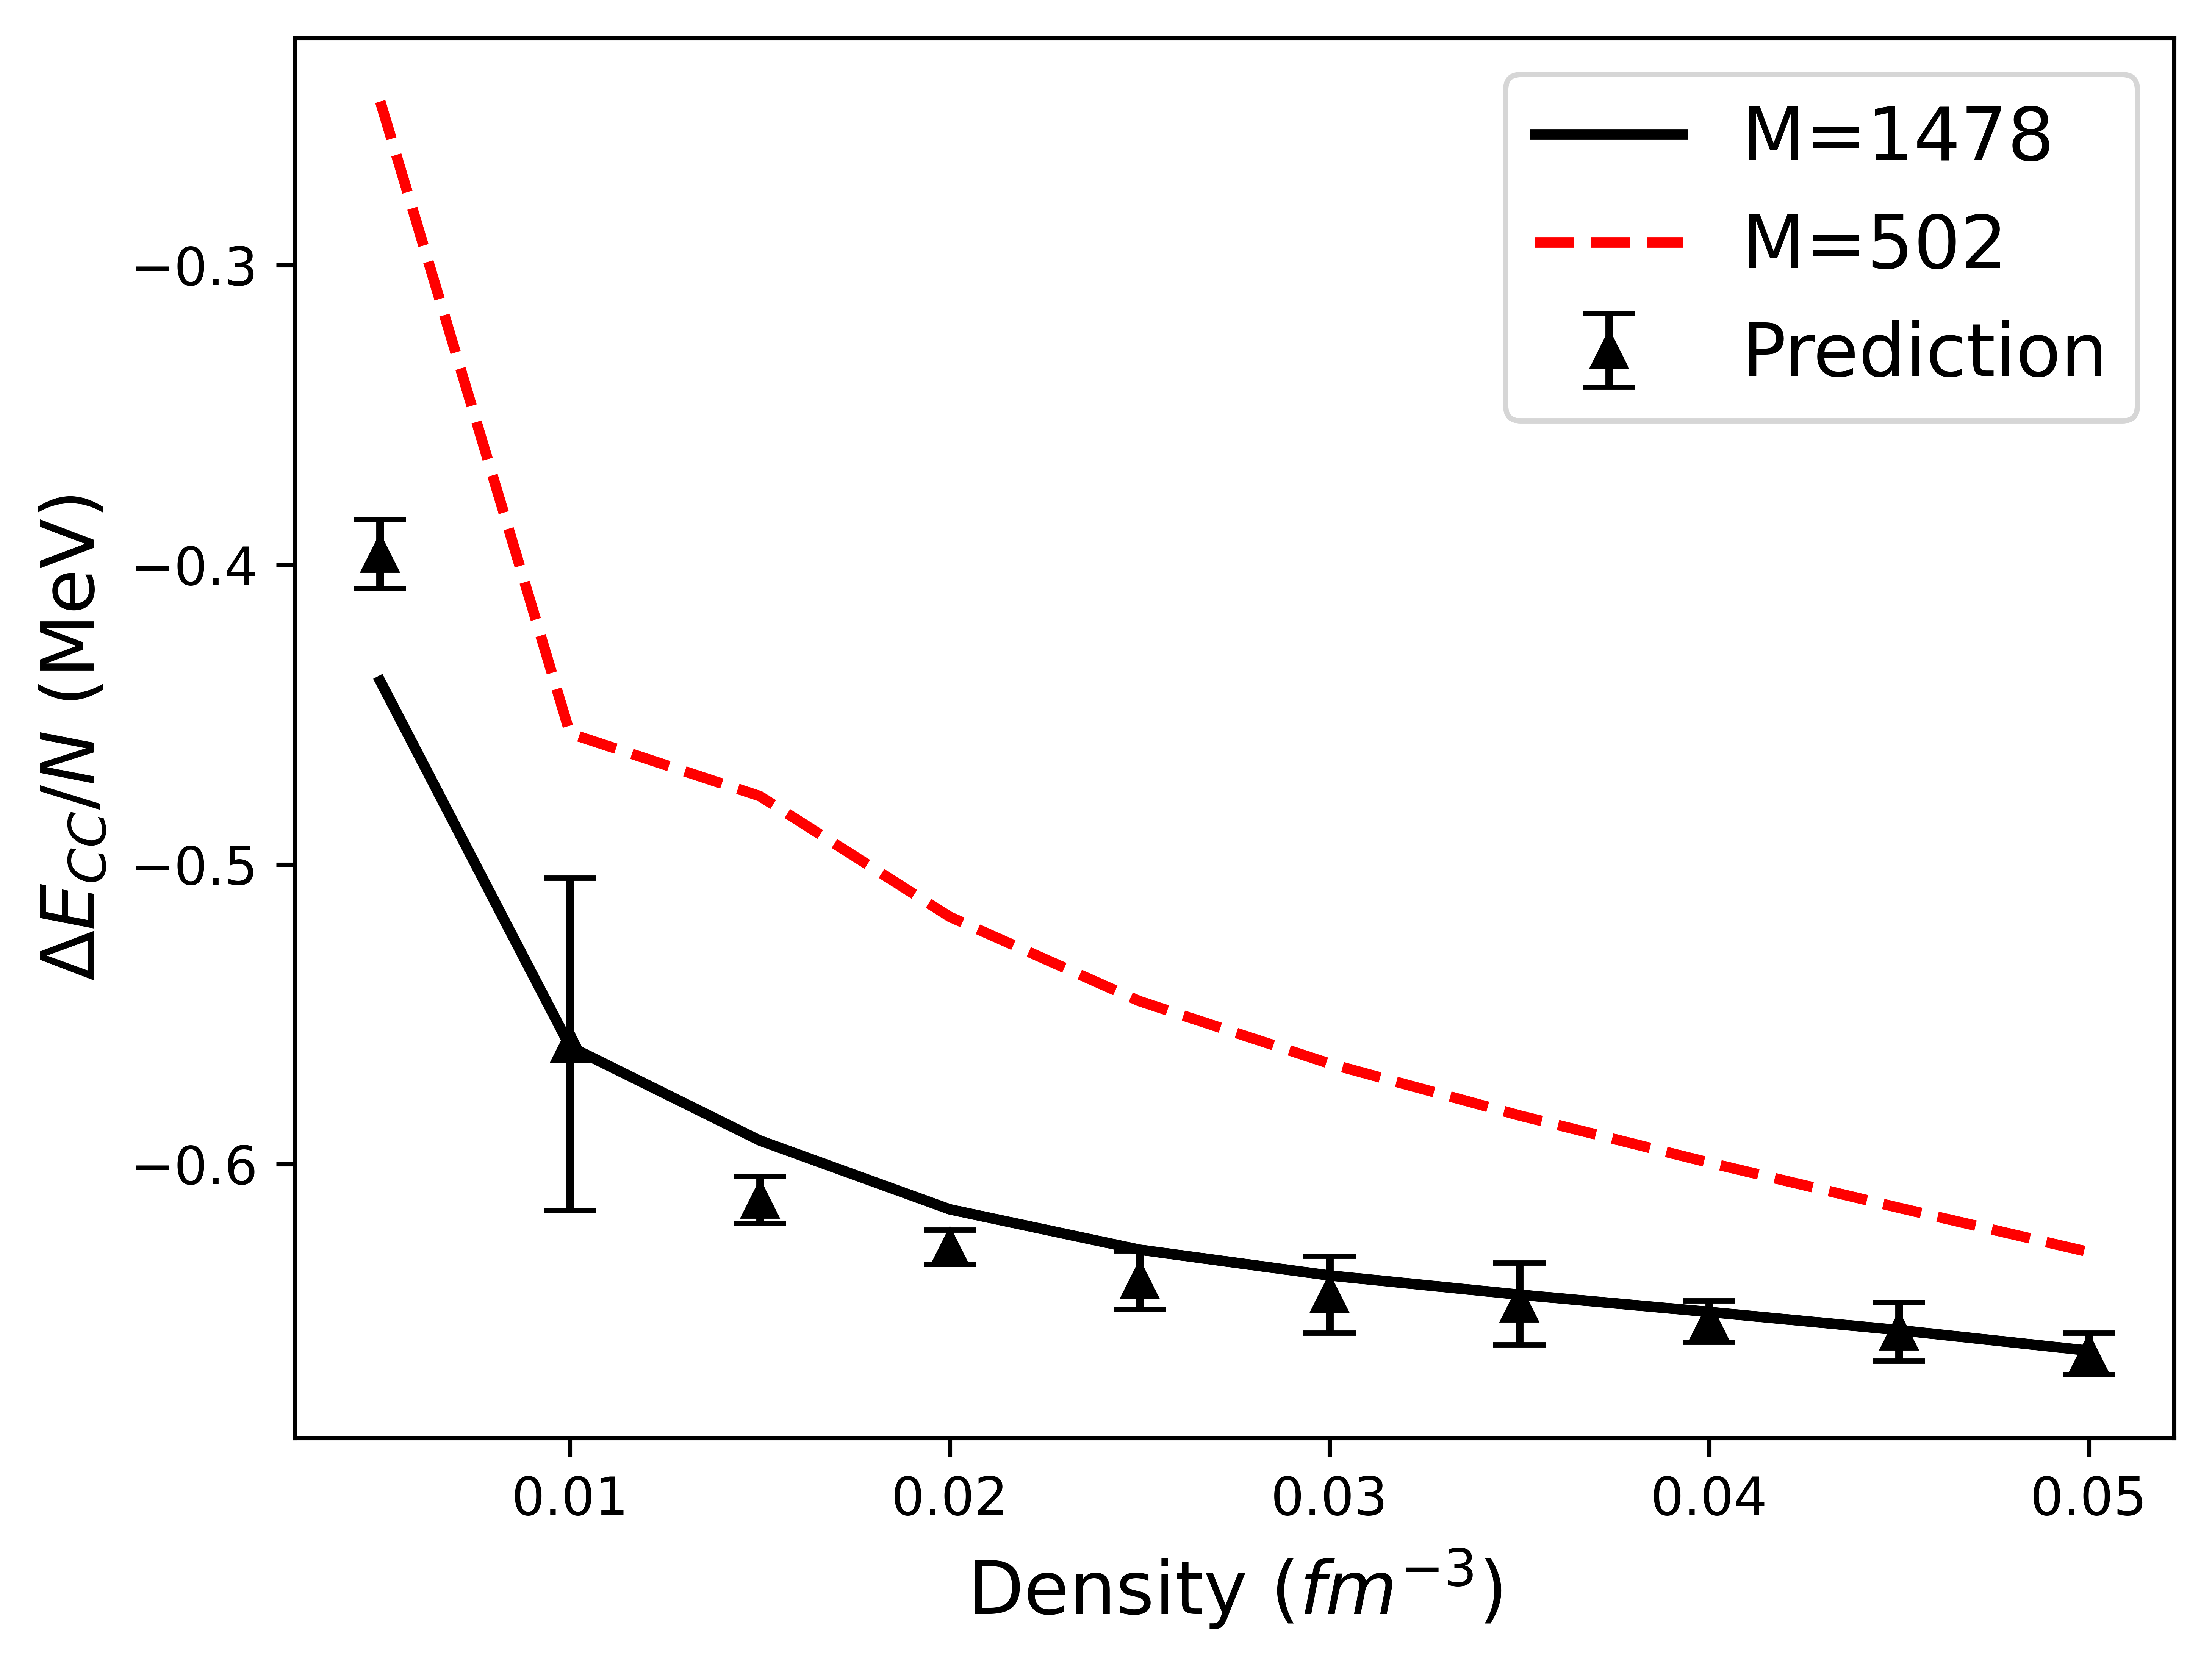
\includegraphics[scale=0.5]{Images/Chapter7/ORNL/neutron_matter_lowdensity-4.png}
  \caption{The results from predicting the converged $\Delta E_{CCD}/N$ for pure neutron matter at low densities.  The average percent error across all densities is 1.90$\%$, and the time savings from generating only the training data versus the fully converged $\Delta E_{CCD}/N$ is 18.27 hours.}
  \label{fig:ornl_pnm_ccd_low}
\end{subfigure}
\caption{The results from predicting the converged $\Delta E_{CC}/N$ for pure neutron matter using the coupled cluster doubles approximation.  Figure (a) shows pure neutron matter for a range of densities around nuclear density (0.10 $\leq$ d $\leq$ 0.20), and figure (b) shows the results for a low-density pure neutron matter (d $\leq$ 0.05). For both graphs, the solid black line plots the fully converged $\Delta E_{CCD}/N$, calculated at 1,478 single-particle states; the triangular markers represent the SRE predictions at each density of interest. The dashed red lines represent the point used to train the GP algorithms with the highest number of single-particle states (M = 186 for Fig. (a) and M = 502 for Fig. (b)) to show that the training set has not reached convergence.}
\label{fig:ornl_pnm_ccd}
\end{figure}

For Figure \ref{fig:pnm_ccd_nuclear}, the average percent error between the fully converged CCD correlation energies and the ML extrapolated CCD correlation energies is 0.25$\%$, and for Figure \ref{fig:ornl_pnm_ccd_low} it is 1.90$\%$. The slightly higher average percent error for the second figure is easily explained. The convergence of the correlation energy is slower at lower densities. Especially at d = 0.005 fm$^{-3}$ and d = 0.01 fm$^{-3}$, the correlation energies had not sufficiently converged at 1,478 single-particle states. This explains why there is a discrepancy between the ML prediction and the complete calculation at d = 0.005fm$^{-3}$. Additionally, the ML prediction at d = 0.01 fm$^{-3}$ closely matches the complete calculations, but there are pretty large error bars on the prediction when compared to the other predictions. This could also be explained by the slow convergence of the correlation energy at this point.

The timing data for \ref{fig:ornl_pnm_ccd} was collected using Michigan State University's high-performance computing center using Intel Xeon compute nodes running at 2.4 GHz and with 200GB of RAM each. For these calculations, 12 MPI nodes were used per calculation. For example, for Figure \ref{fig:pnm_ccd_nuclear}, generating the six fully converged CCD correlation energies at M = 1,478 single particle states took 13.03 hours. However, generating the training data for the six GP algorithms took only 0.32 hours, leading to a time savings of using the ML extrapolations of 12.71 hours. Additionally, for Figure \ref{fig:ornl_pnm_ccd_low}, it takes 24.16 hours to generate all ten fully converged CCD correlation energies and M = 1,478 single-particle states. However, it only takes 5.88 hours to generate the ten GP training data sets. Therefore using the ML extrapolation over doing the complete calculations saves 18.27 hours.

When considering both the accuracy and the time savings, the SRE method applied to CCD calculations of pure neutron matter with chiral potentials appears successful. The CCD correlation energies per particle can be accurately recreated for all but the smallest densities with very little training data and significant time savings.


\begin{figure}
    \centering
    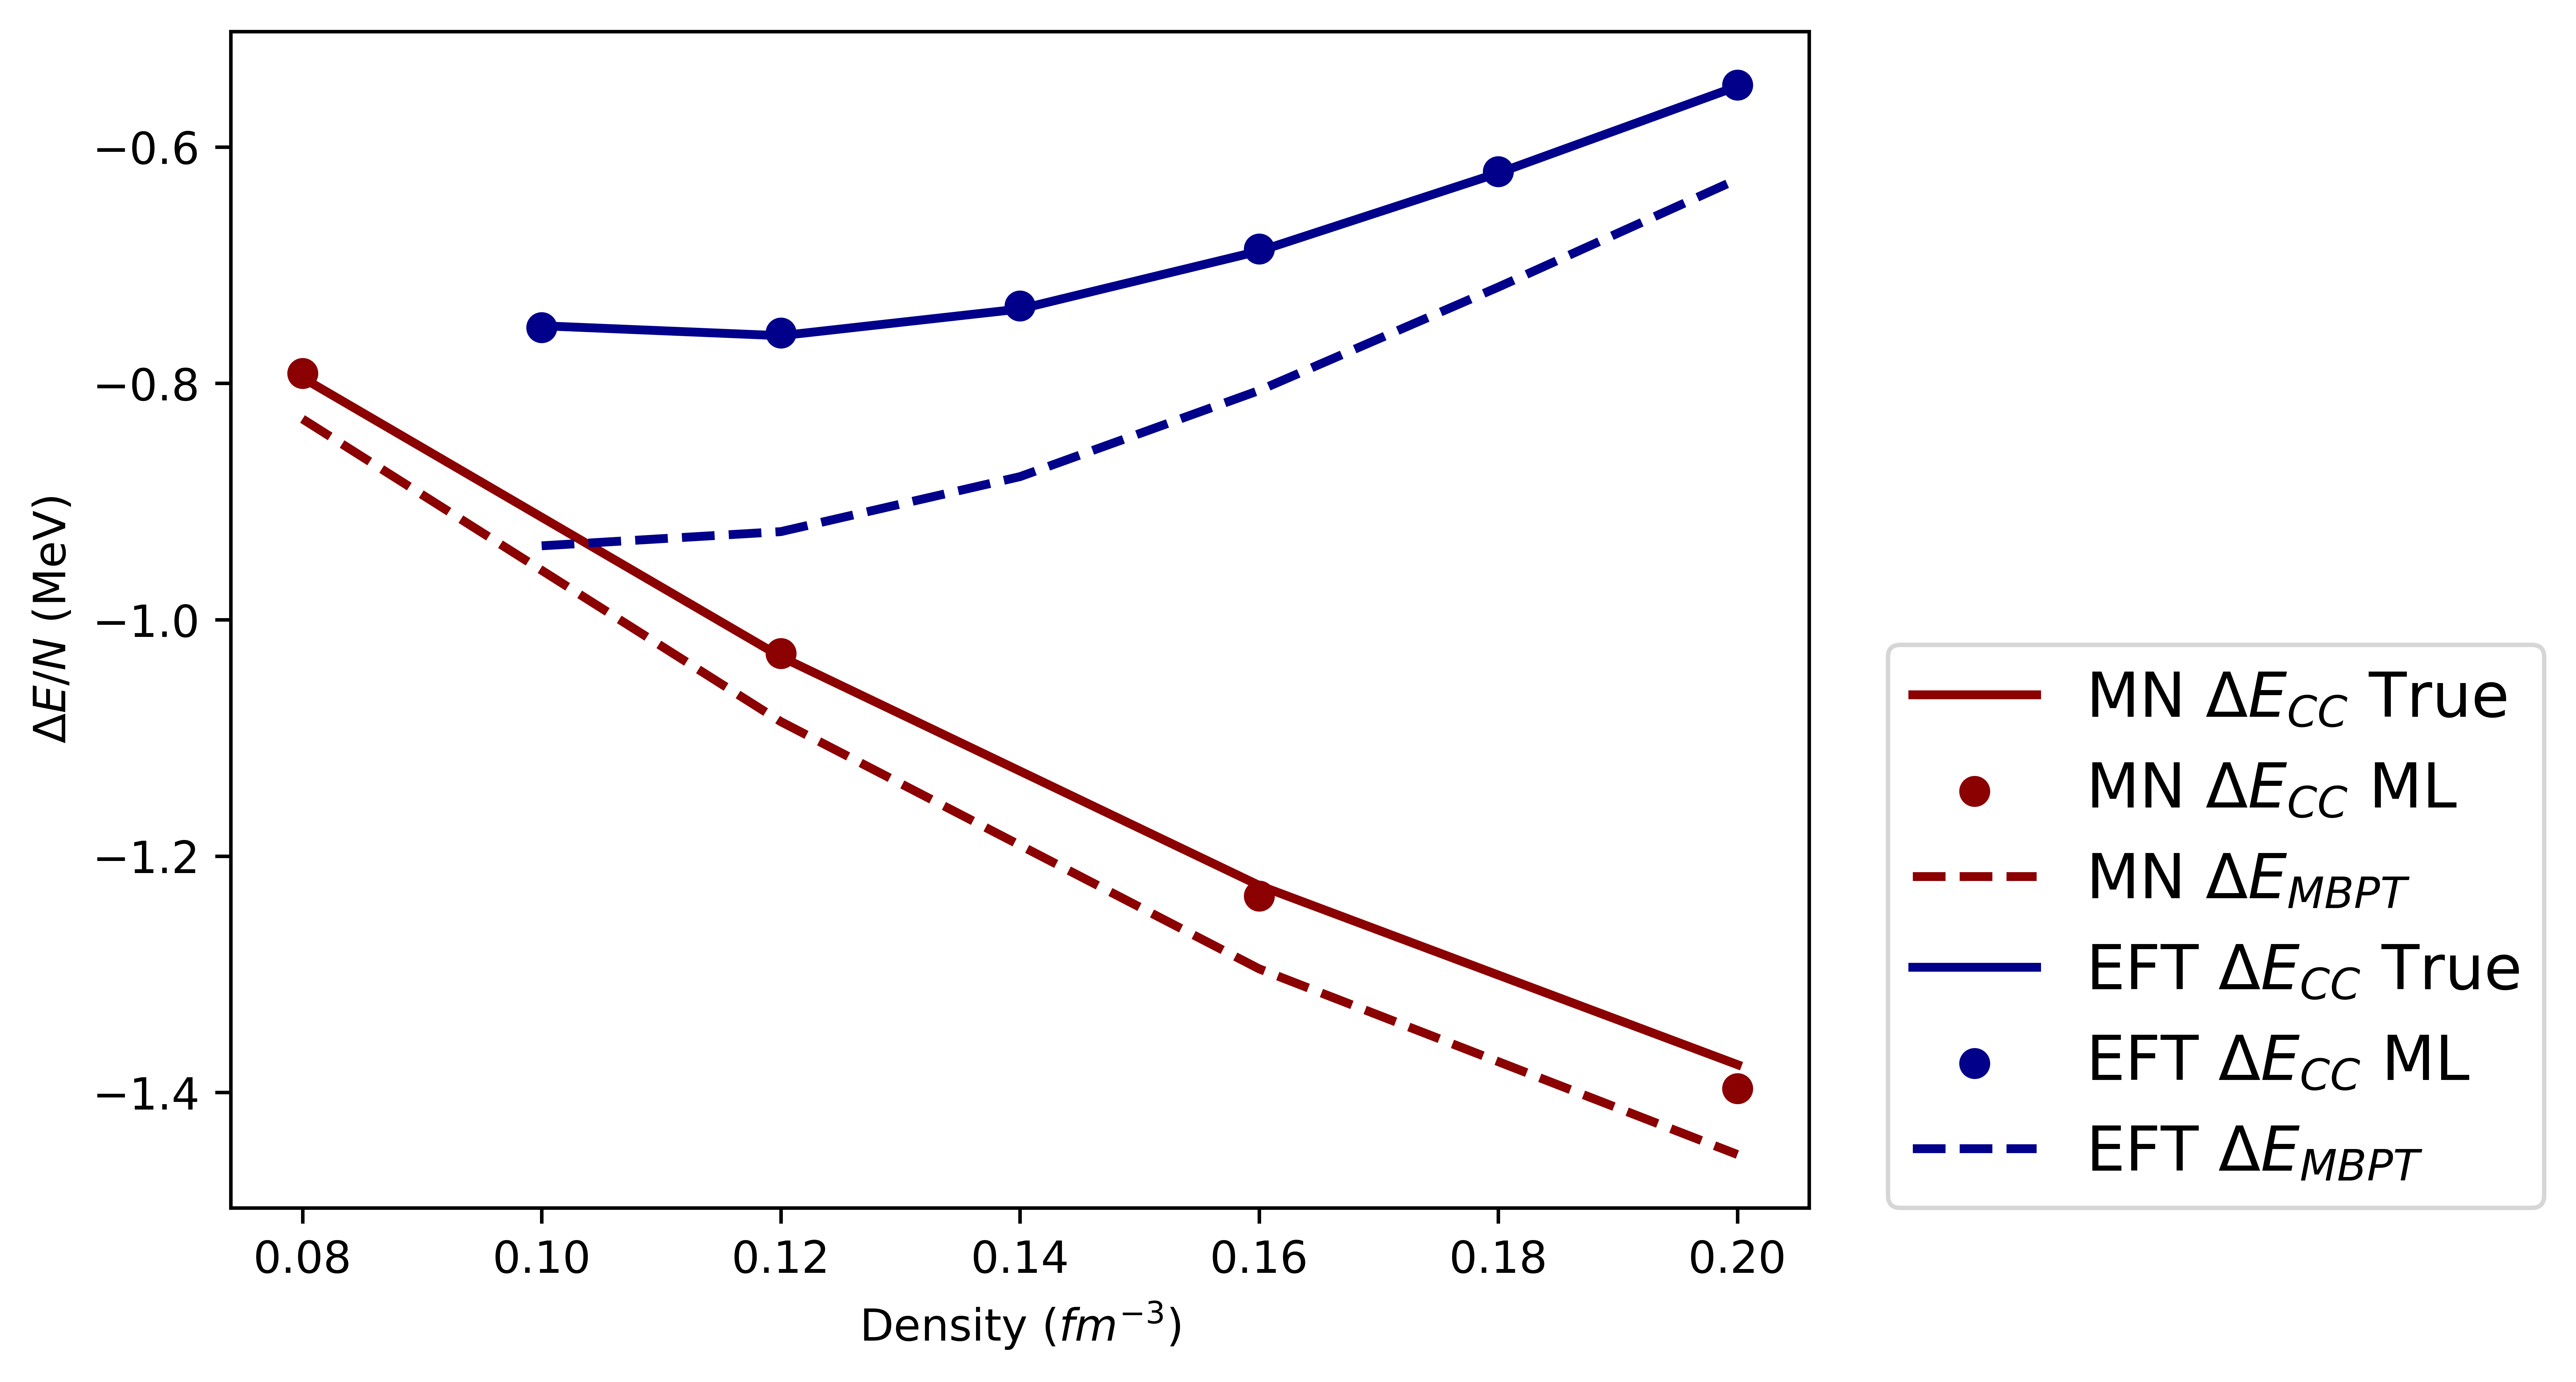
\includegraphics[scale=0.75]{Images/Chapter7/ORNL/EFT_and_MN.png}
    \caption{A comparison of correlation energy calculations for pure neutron matter near nuclear density for 66 neutrons.  The red data sets were calculated with the Minnesota potential, and the blue data sets with the chiral potentials. The dashed lines represent the converged correlation energy per particle from MBPT2, the solid lines represent the converged CCD correlation energies per particle, and the circular makers represent the ML predictions for the converged CCD correlation energies per particle.}
    \label{fig:eft_vs_mn}
\end{figure}

Figure \ref{fig:eft_vs_mn} compares pure neutron matter converged correlation energies per particle calculated with MBPT2 and CCD and for the Minnesota and chiral potentials. The Minnesota potential results are from calculations performed at 6,142 single-particle states of 70 total energy shells, and the chiral potential results are from 1,478 single-particle states or 27 energy shells. However, both the MBPT2 and CCD correlations energies have sufficiently converged. The ML predictions for the converged CCD correlation energy per particle are also shown. The results shown are for calculations involving 66 neutrons and near nuclear density. There are a few critical observations we can make from this graph. First, we know that the Minnesota and chiral potentials will produce different results as they model the nuclear interaction differently and to different levels of accuracy. The results differ significantly, with the chiral potentials yielding lower energy for both MBPT2 and CCD calculations.
Additionally, the difference in the results increases as density increases, indicating that there will be quite a significant difference between the two potentials at densities greater than nuclear density. Secondly, we can look at the difference between the MBPT2 and CCD results for the two potentials. For both potentials, the MBPT2 correlation energy per particle is lower than the CCD correlation energy per particle. However, for the Minnesota potential, the MBPT2 correlation energies are only slightly below the CCD correlation energies, and the gap between the MBPT2 correlation energies and the CCD correlation energies is roughly consistent over the entire density range shown. There is a more significant discrepancy between the MBPT2 and CCD correlation energies for the chiral potential, and this gap grows as the density decreases. Finally, it is essential to note that for each potential, the ML predictions to the converged CCD correlations energies are in good agreement with the total calculations, so the SRE method is potential independent.

        Beyond the CCD approximation, we can also look at the CCDT-1 coupled-cluster approximation, adding some aspects of the $\hat{T}_3$ excitation operator into the calculations without the full-time needed for a complete CCDT calculation. In the next section, we will also consider the CCD(T) approximation, another coupled-cluster approximation that adds some aspects of the $\hat{T}_3$ operator into the calculations using a different algorithm.

First, we should verify that the CCDT-1 approximation with the same NNLO chiral potentials gives a different (and more accurate) approximation than the CCD approximation for pure neutron matter. In Fig. \ref{fig:ccd_vs_ccdt1}, the CCD correlation energies per particle are plotted as a function of the density of the pure neutron matter system for 66 neutrons and at densities around nuclear density with the solid red line. The CCD calculations shown were performed at 1,478 single-particle states, where the calculations converged. For the CCDT-1 calculations, shown with the solid black line, the calculations were also performed with the NNLO chiral potentials for pure neutron matter and 66 neutrons and at densities around nuclear density. As a result, the correlation energy calculations using CCDT-1 converge much faster than for CCD and only need 514 single-particle states to reach convergence. Additionally, since CCDT-1 calculations scale as $O(M^7)$ compared to a CCD calculation at $O(M^6)$, performing CCDT-1 calculation at higher values of M is computationally prohibitive. As shown in Fig \ref{fig:ccd_vs_ccdt1}, the CCD and CCDT-1 approximations give significantly different predictions for the correlation energies at each density value shown.

\begin{figure}
    \centering
    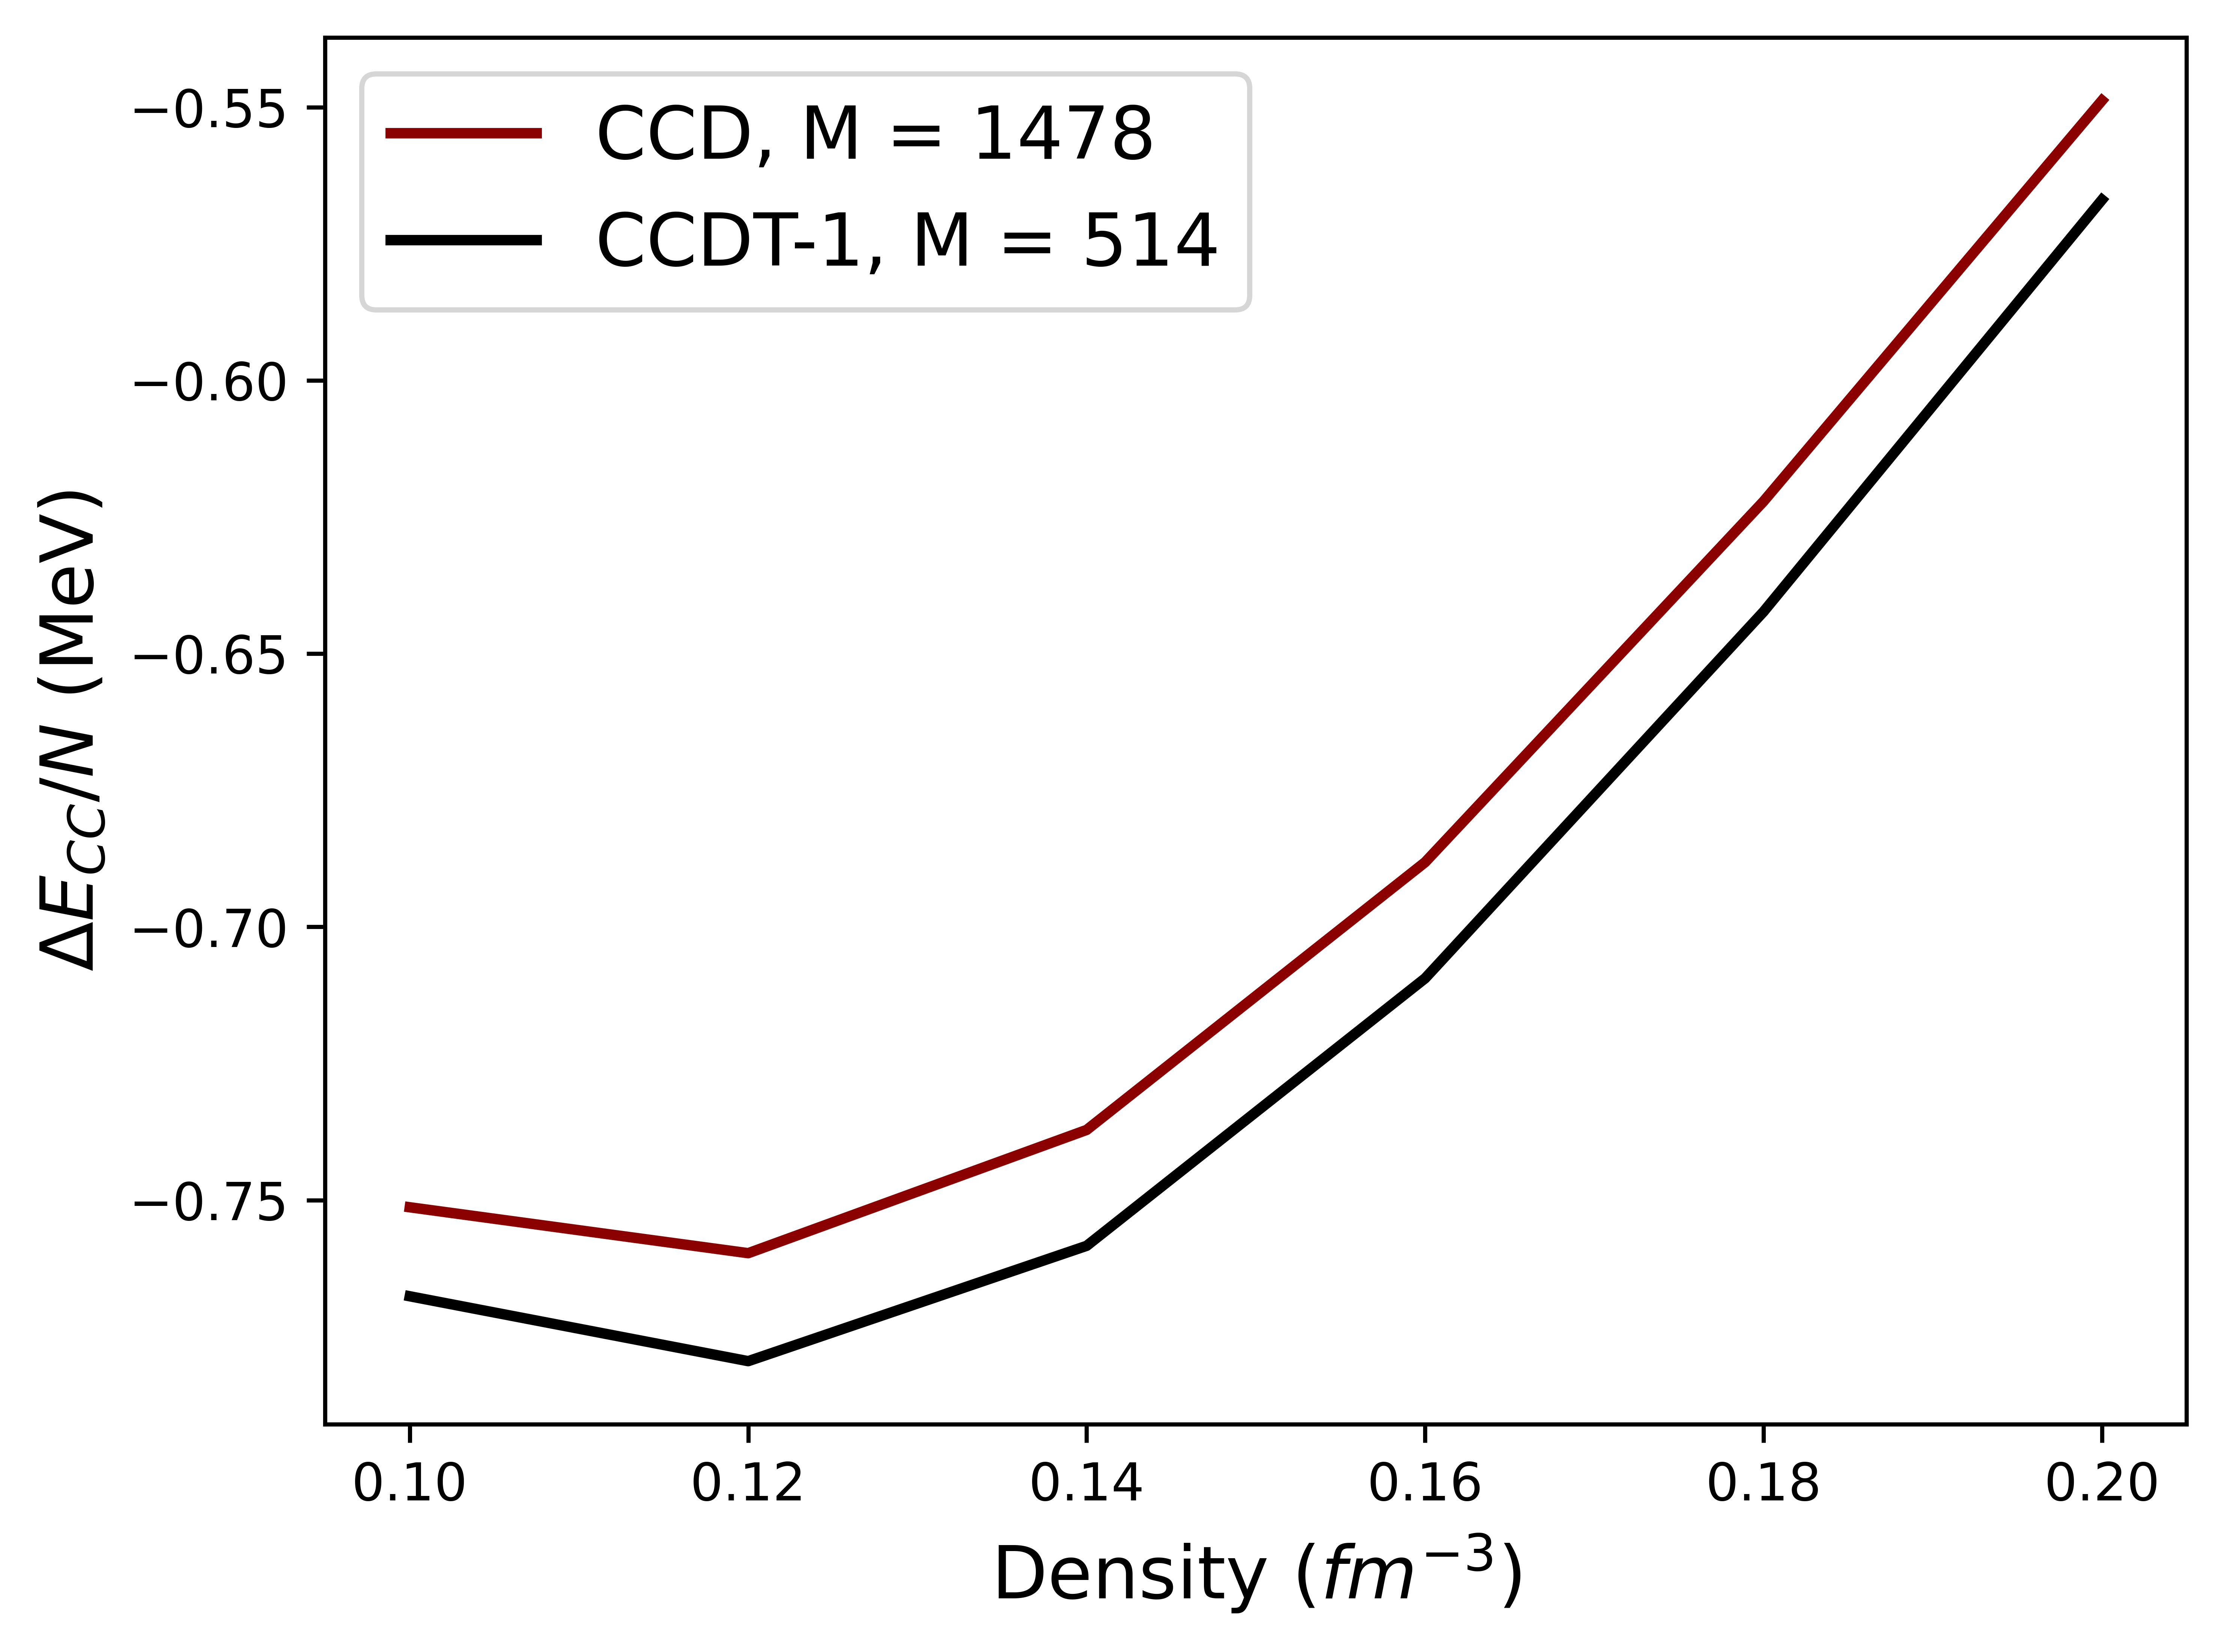
\includegraphics[scale=0.75]{Images/Chapter7/ORNL/ccdt1_nuclear_neutron_matter_no_ML.png}
    \caption{A comparison between the CCD and CCDT-1 correlation energies for a pure neutron matter system (N = 66 neutrons) with NNLO chiral potentials and for densities around nuclear density.  The CCDT-1 approximation consistently gives a lower correlation energy than CCD correlation energy at all densities in the graph.}
    \label{fig:ccd_vs_ccdt1}
\end{figure}

We can also compare the run times needed to complete a CCDT-1 calculation over a CCD calculation. Fig. \ref{fig:ccd_ccdt1_times} shows the total run time needed to complete a CCDT-1 calculation on Michigan State University's High-Performance Computing Center using Intel Xeon nodes with a clock speed of 2.4 GHz and 24 MPI nodes per run. The results in this figure were collected by performing CCDT-1 calculations on a pure neutron matter system with chiral NNLO potentials and with 66 neutrons and a density of 0.16 fm$^{-3}$. The results are reported in node hours. It is obvious that the run time increases very quickly with the number of single-particle states in the calculation. This rapid increase in run time is even more apparent if we plot the CCD and CCDT-1 run times on the same plot, as in Fig. \ref{fig:ccd_ccdt1_times}.  Though the CCDT-1 calculation converges at a smaller number of single-particle states, the total run time needed is drastically higher than that needed for the CCD calculations. At 514 single-particle states, the CCDT-1 calculation takes over 15 times longer than the CCD calculation at the same number of single-particle states. So even though we were motivated to use the SRE method to save time on the CCD calculations with the chiral NNLO potentials due to their run times, there is even more of a need for an accurate extrapolation method for the CCDT-1 calculations as their run times are an order of magnitude larger.

\begin{figure}
    \centering
    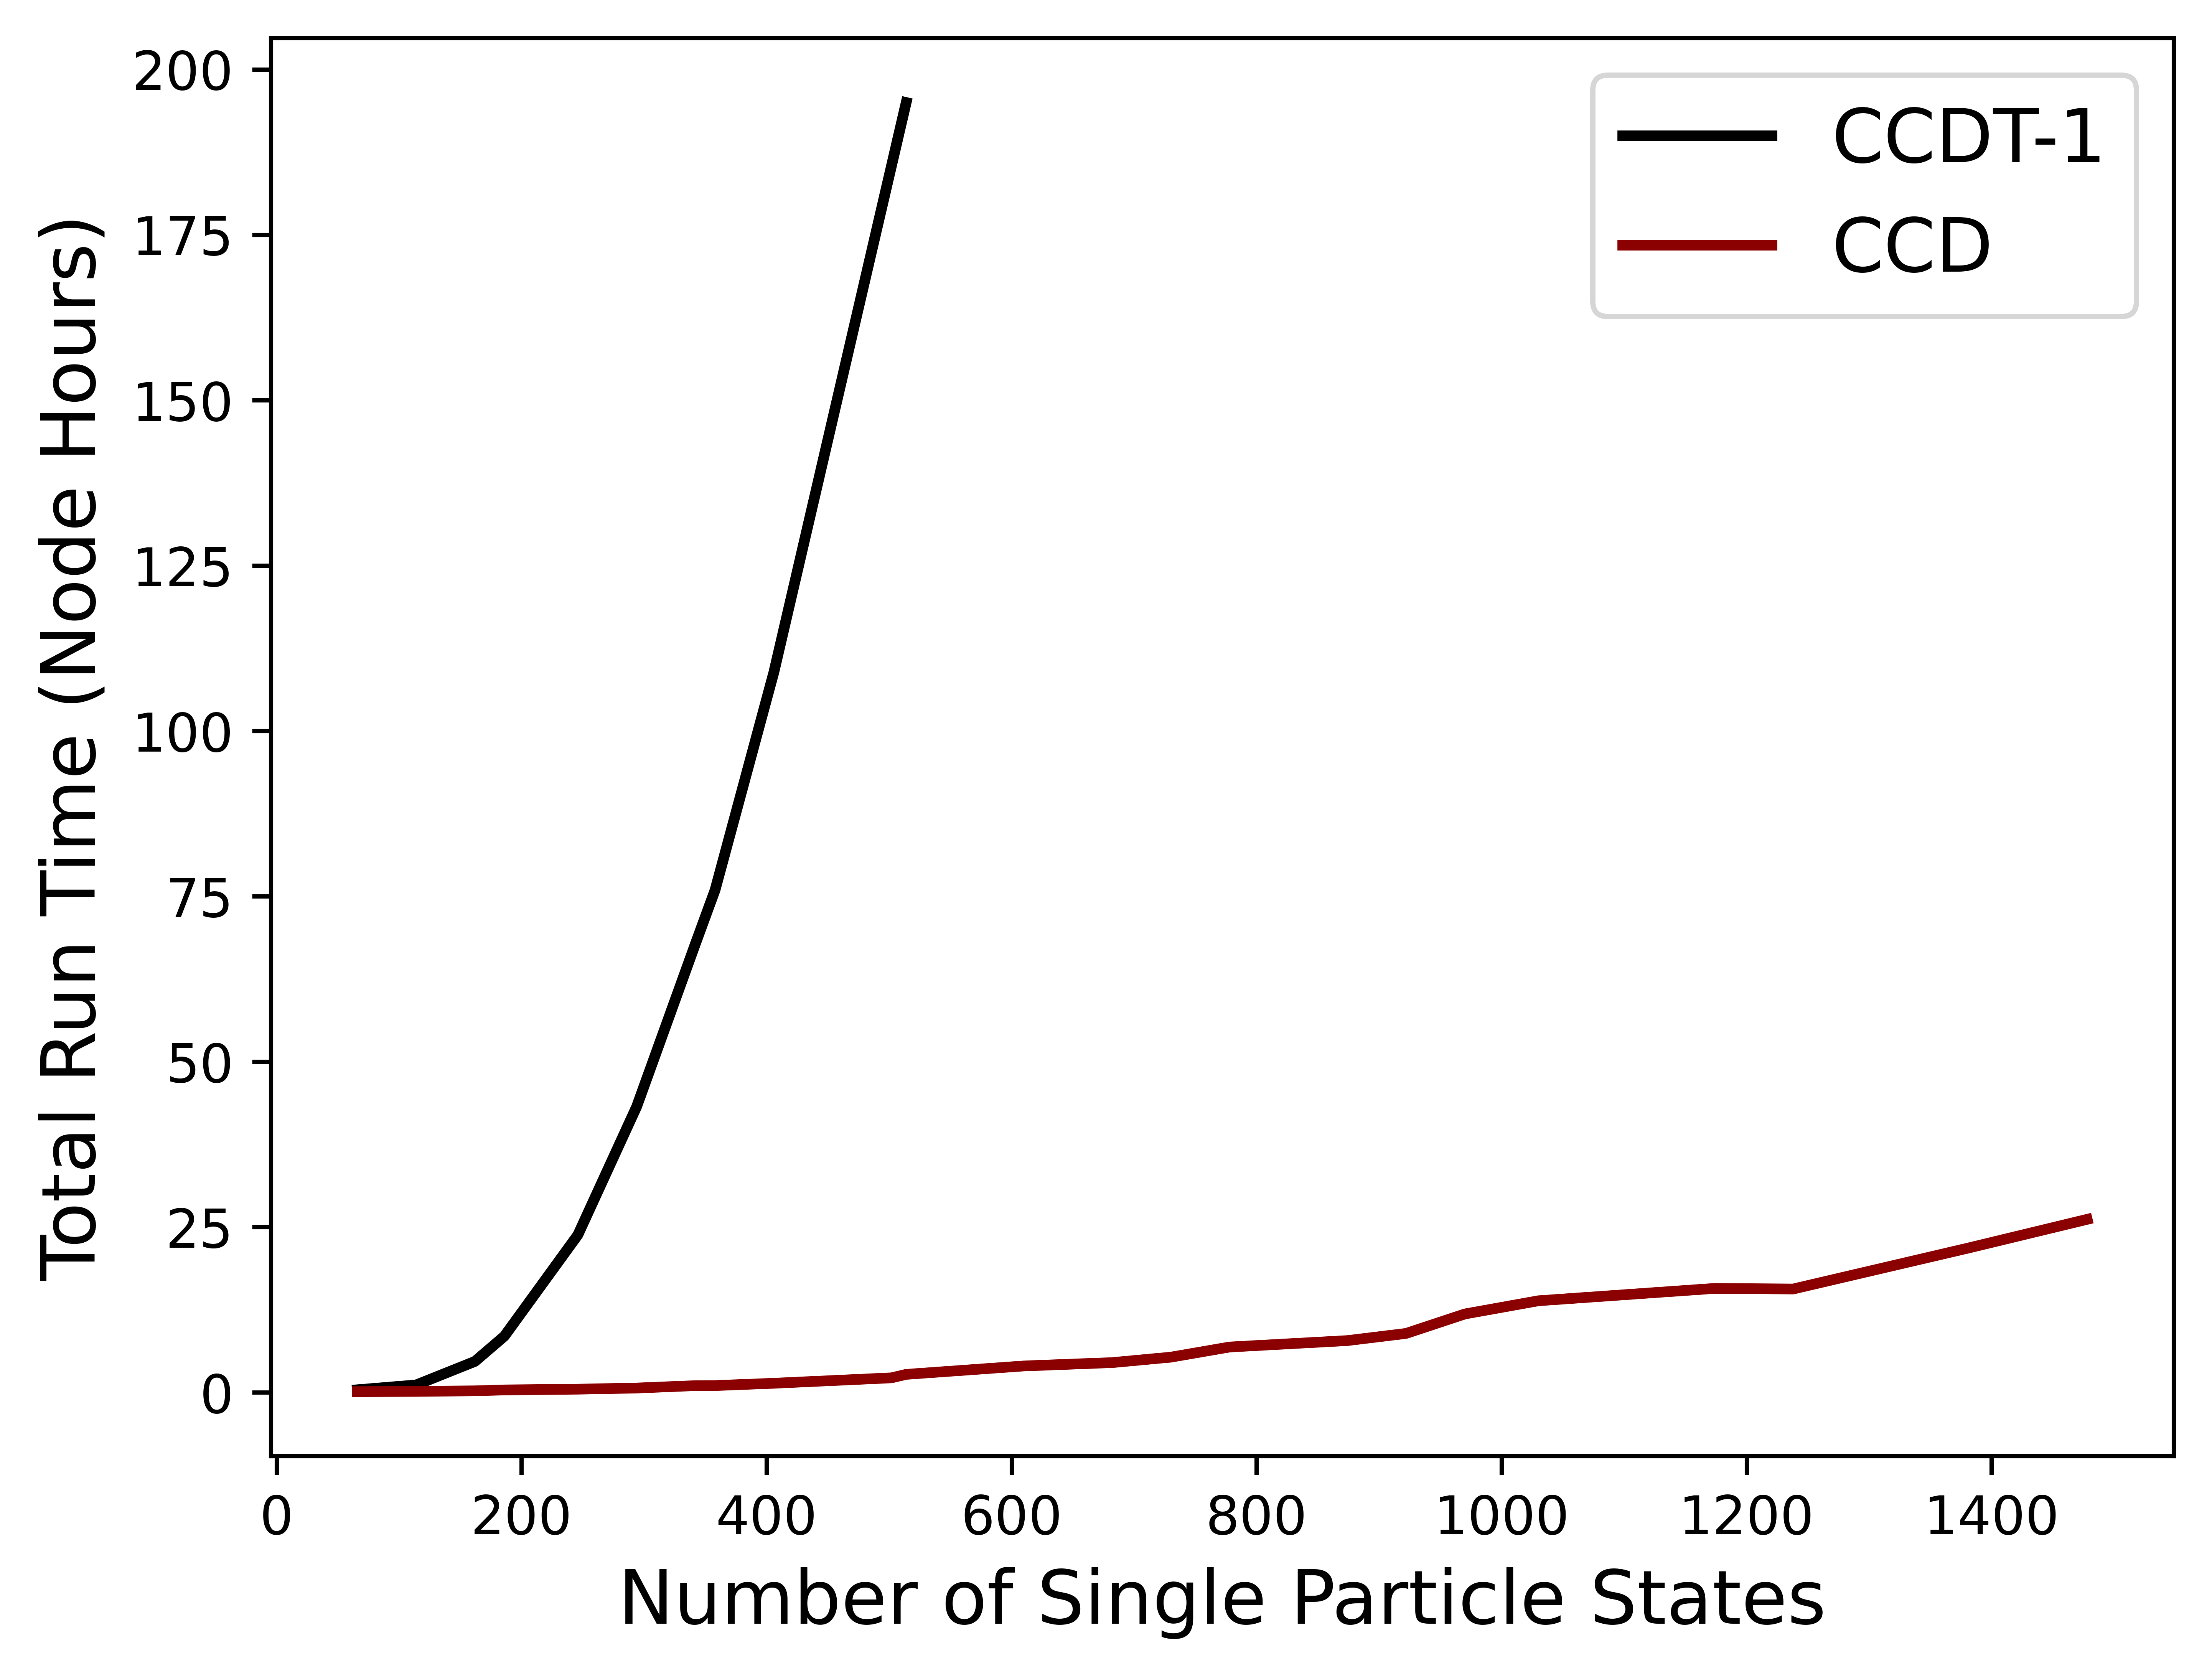
\includegraphics{Images/Chapter7/ORNL/ccdt1 and ccd times.png}
    \caption{The run times needed to complete CCD and CCDT-1 calculations for a PNM system reported in node hours.}
    \label{fig:ccd_ccdt1_times}
\end{figure}

Next, we will look at the feasibility of predicting the CCDT-1 correlation energy from the MBPT2 correlation energy using the same SRE and machine learning setup as the above doubles predictions. We will use the SRE method described in section 6.4.1 to predict the CCDT-1 correlation energies from the MBPT2 correlation energies using three training points (from one to three open shells or 114 to 186 single particle states) with a sequence length of 1 and a Gaussian process algorithm with its alpha value set to the standard deviation of the training data to the fourth power.

Fig. \ref{fig:one_ccdt1_density} shows the results of predicting the converged CCDT-1 correlation energies using the method described above for a pure neutron matter system with 66 neutrons and d = 0.16 fm$^{-3}$. For the plot, the complete calculations are shown with solid lines, the training data with points, and the SRE predicted converged correlation energy with the horizontal dashed line. The percent error between the converged $\Delta E_{CCDT1}$ that has been fully calculated at 514 single particle states and the SRE prediction is 0.51$\%$. As a comparison, the percent error between the converged $\Delta E_{CCDT1}$ that has been fully calculated at 514 single particle states and the largest point in the training data (at 186 single particle states) is 12.19$\%$. This means that in the time needed to generate the training data, which is 14.29 node hours for the three points, the accuracy of the correlation energy can be improved from 12.19$\%$ to just 0.51$\%$. Furthermore, the time needed to calculate the fully converged correlation energy at 514 single-particle states is 194.97 node hours, meaning that just for this one density, the SRE method saves 180.68 node hours while only sacrificing 0.51$\%$ in accuracy. All timing data presented in this section was collected with a Fortran code run on Michigan State University's High-Performance Computing Center on Intel Xeon processors with a 2.4 GHz clock speed and 24 MPI nodes.

\begin{figure}
    \centering
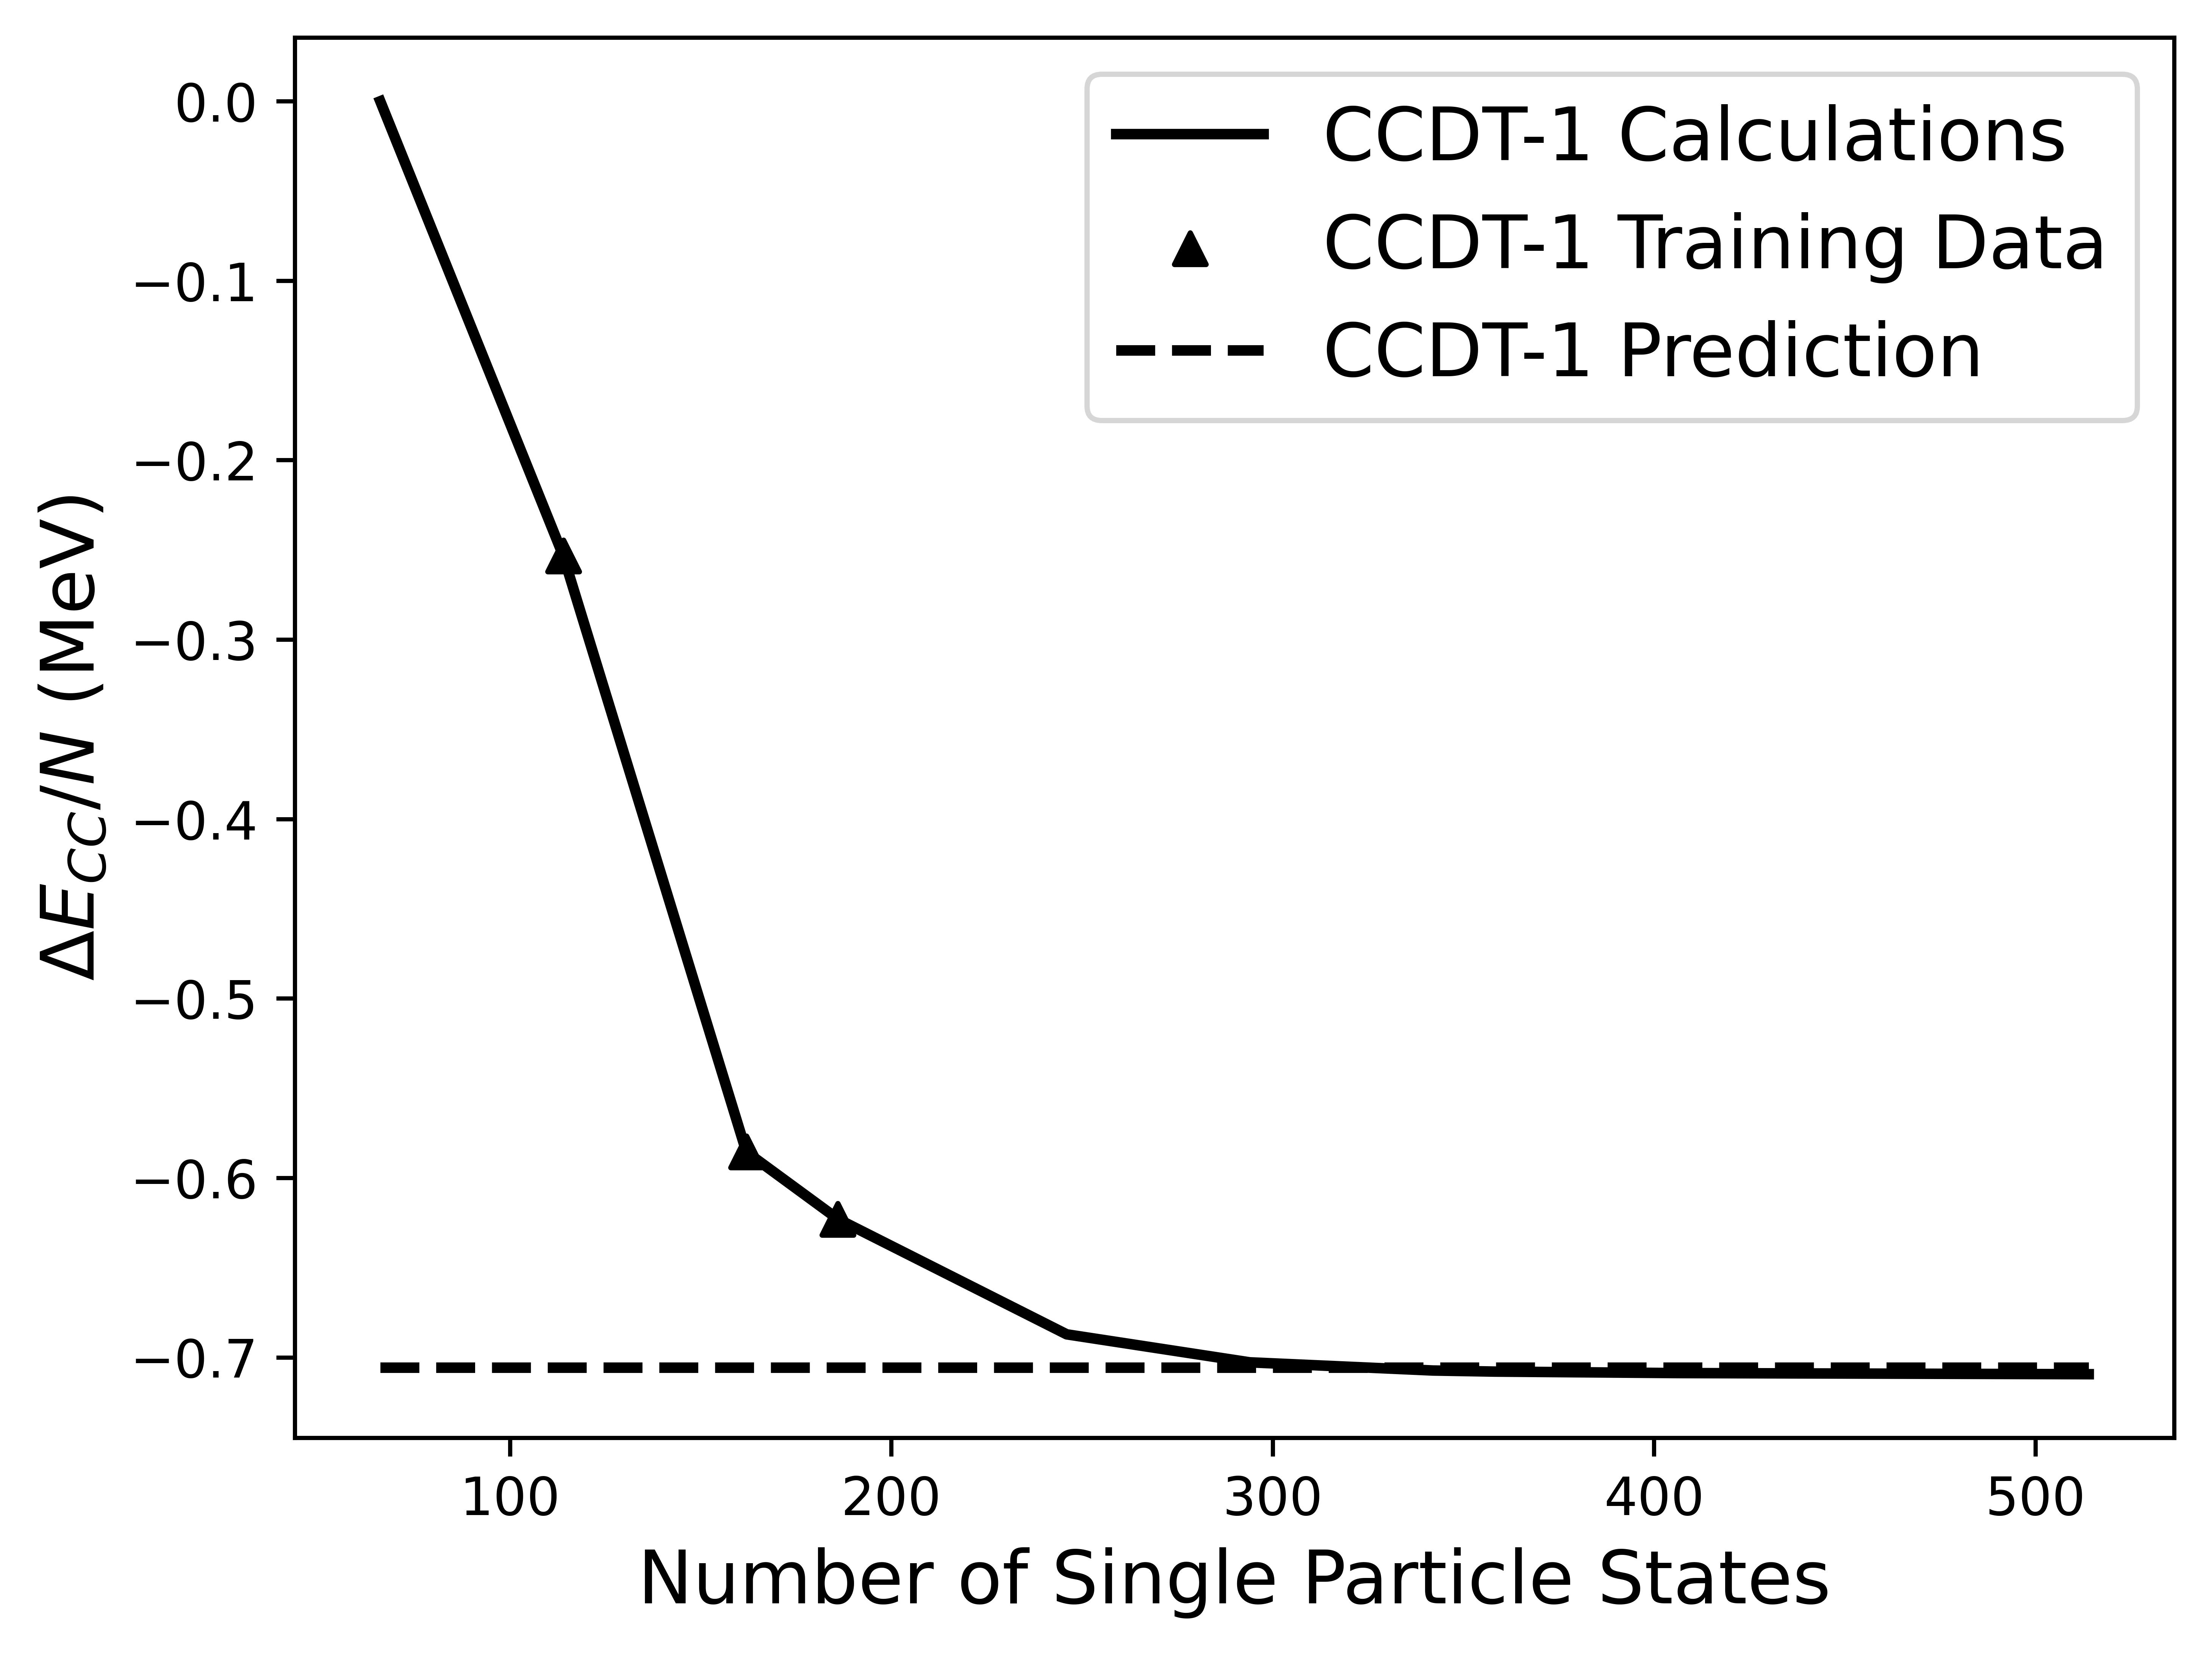
\includegraphics[scale=0.75]{Images/Chapter7/ORNL/CCDT1_Initial.png}
    \caption{The results performing coupled-cluster calculations with the CCDT-1 approximation on a pure neutron matter system with chiral NNLO potentials, 66 neutrons, and d = 0.16 fm$^{-3}$. The full calculations are shown with a solid line, the training data used for the SRE algorithm is shown with the triangular markers, and the SRE prediction for the converged correlation energy is shown with the dashed line. The percent error between the SRE prediction and the fully calculated converged correlation energy is 0.51$\%$, and the time savings for performing the SRE method is 180.68 node hours.}
    \label{fig:one_ccdt1_density}
\end{figure}

Now that we have shown that the SRE method can be feasibly applied to predict converged CCDT-1 correlation energies using only the MBPT2 energies, we can use this method to predict the correlation energies at various densities. Fig. \ref{fig:pnm_ccdt1_nuclear} compares the correlation energies from the last point in the training data at M = 186 (red dashed line), the fully calculated converged $\Delta E_{CCDT1}$ at 514 single-particle states (black line), and the SRE prediction for the converged correlation energies at densities around nuclear density. We can see that the training data is far from the converged values, and in fact, the difference between the M = 186 plot and the M = 514 plot is highest at the lower densities shown here. This is to show that the correlation energies used to train the SRE algorithm are not converged, and thus, a noticeable improvement is made over just using the training data. For Fig. \ref{fig:pnm_ccdt1_nuclear}, the average percent error between the SRE predictions and the complete calculations is 0.45$\%$. Furthermore, the total computational time saved when generating the six data points with the SRE method over fully generating them at 514 single-particle states is 917.30 node hours.

\begin{figure}
  \centering
  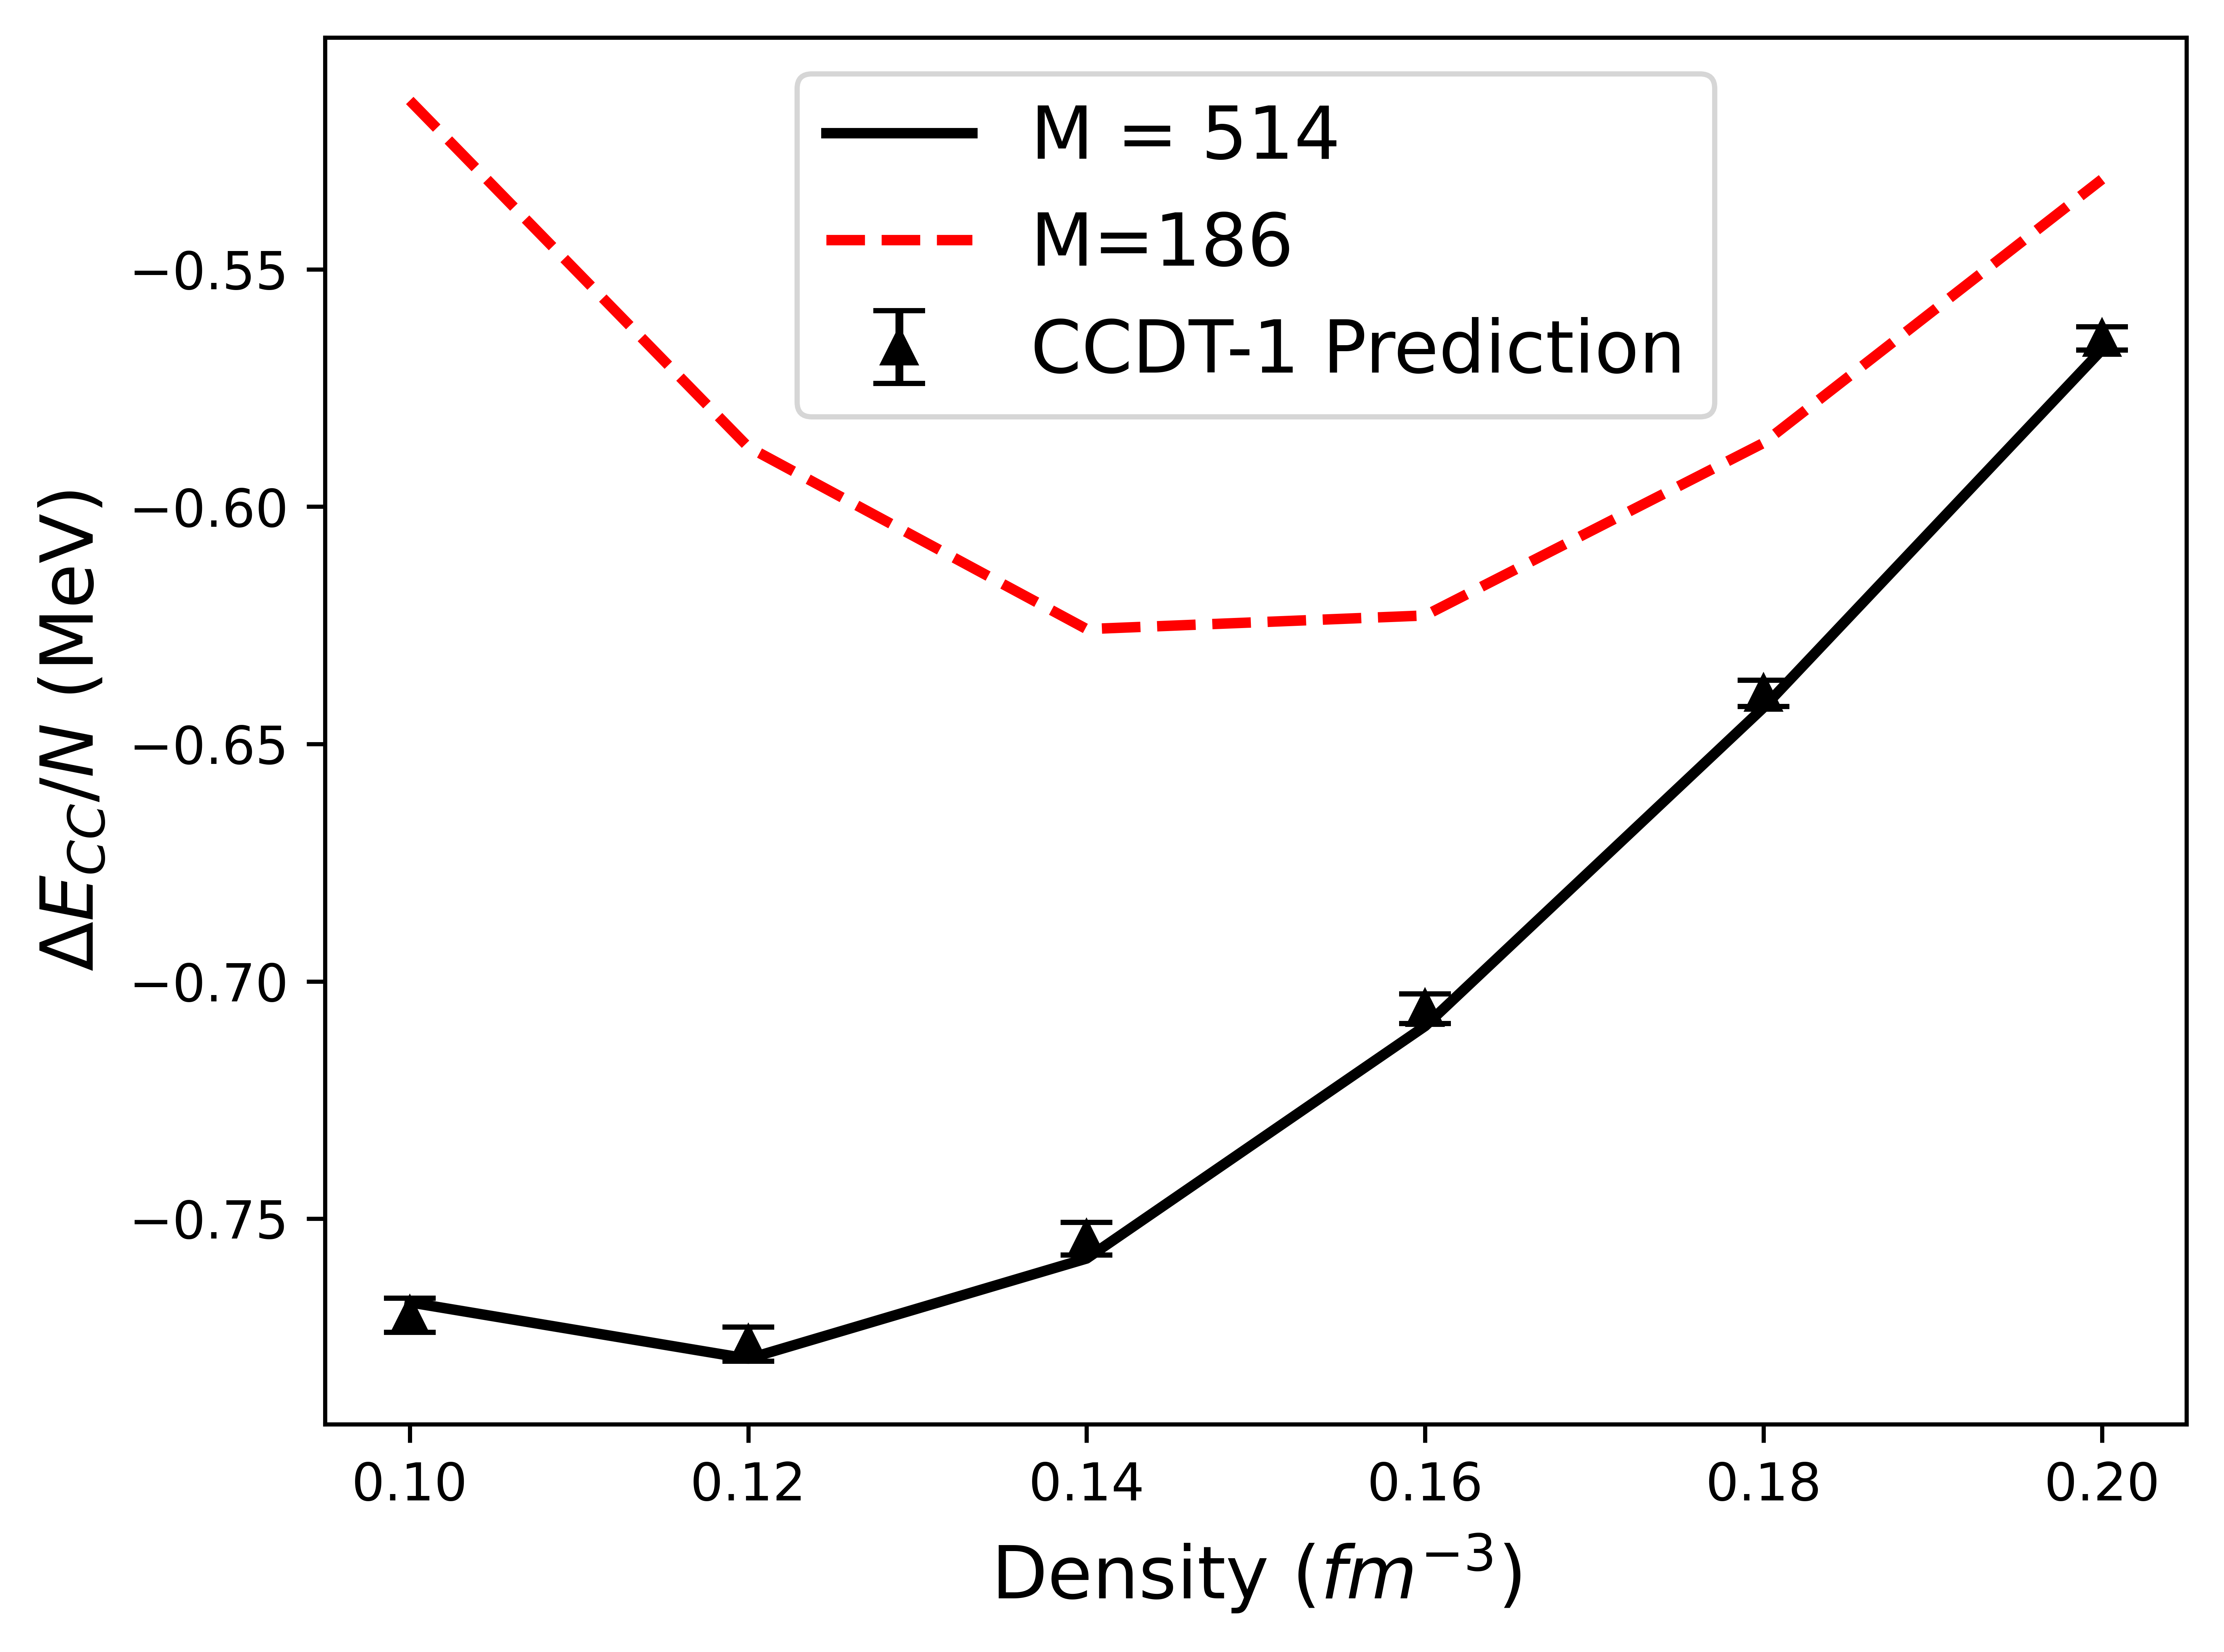
\includegraphics[scale=0.5]{Images/Chapter7/ORNL/ccdt1_nuclear_neutron_matter_with_training.png}
  \caption{The results from predicting the converged $\Delta E_{CCDT1}/N$ for pure neutron matter at densities around nuclear density.  The average percent error across all densities is 0.45$\%$, and the time savings from generating only the training data versus the fully converged $\Delta E_{CCDT1}/N$ is 917.30 node hours.}  \label{fig:ccdt1_nuclear_density}
\end{figure}

Finally, let us compare the CCDT-1 results to the CCD results for densities around nuclear density.

\begin{figure}
    \centering
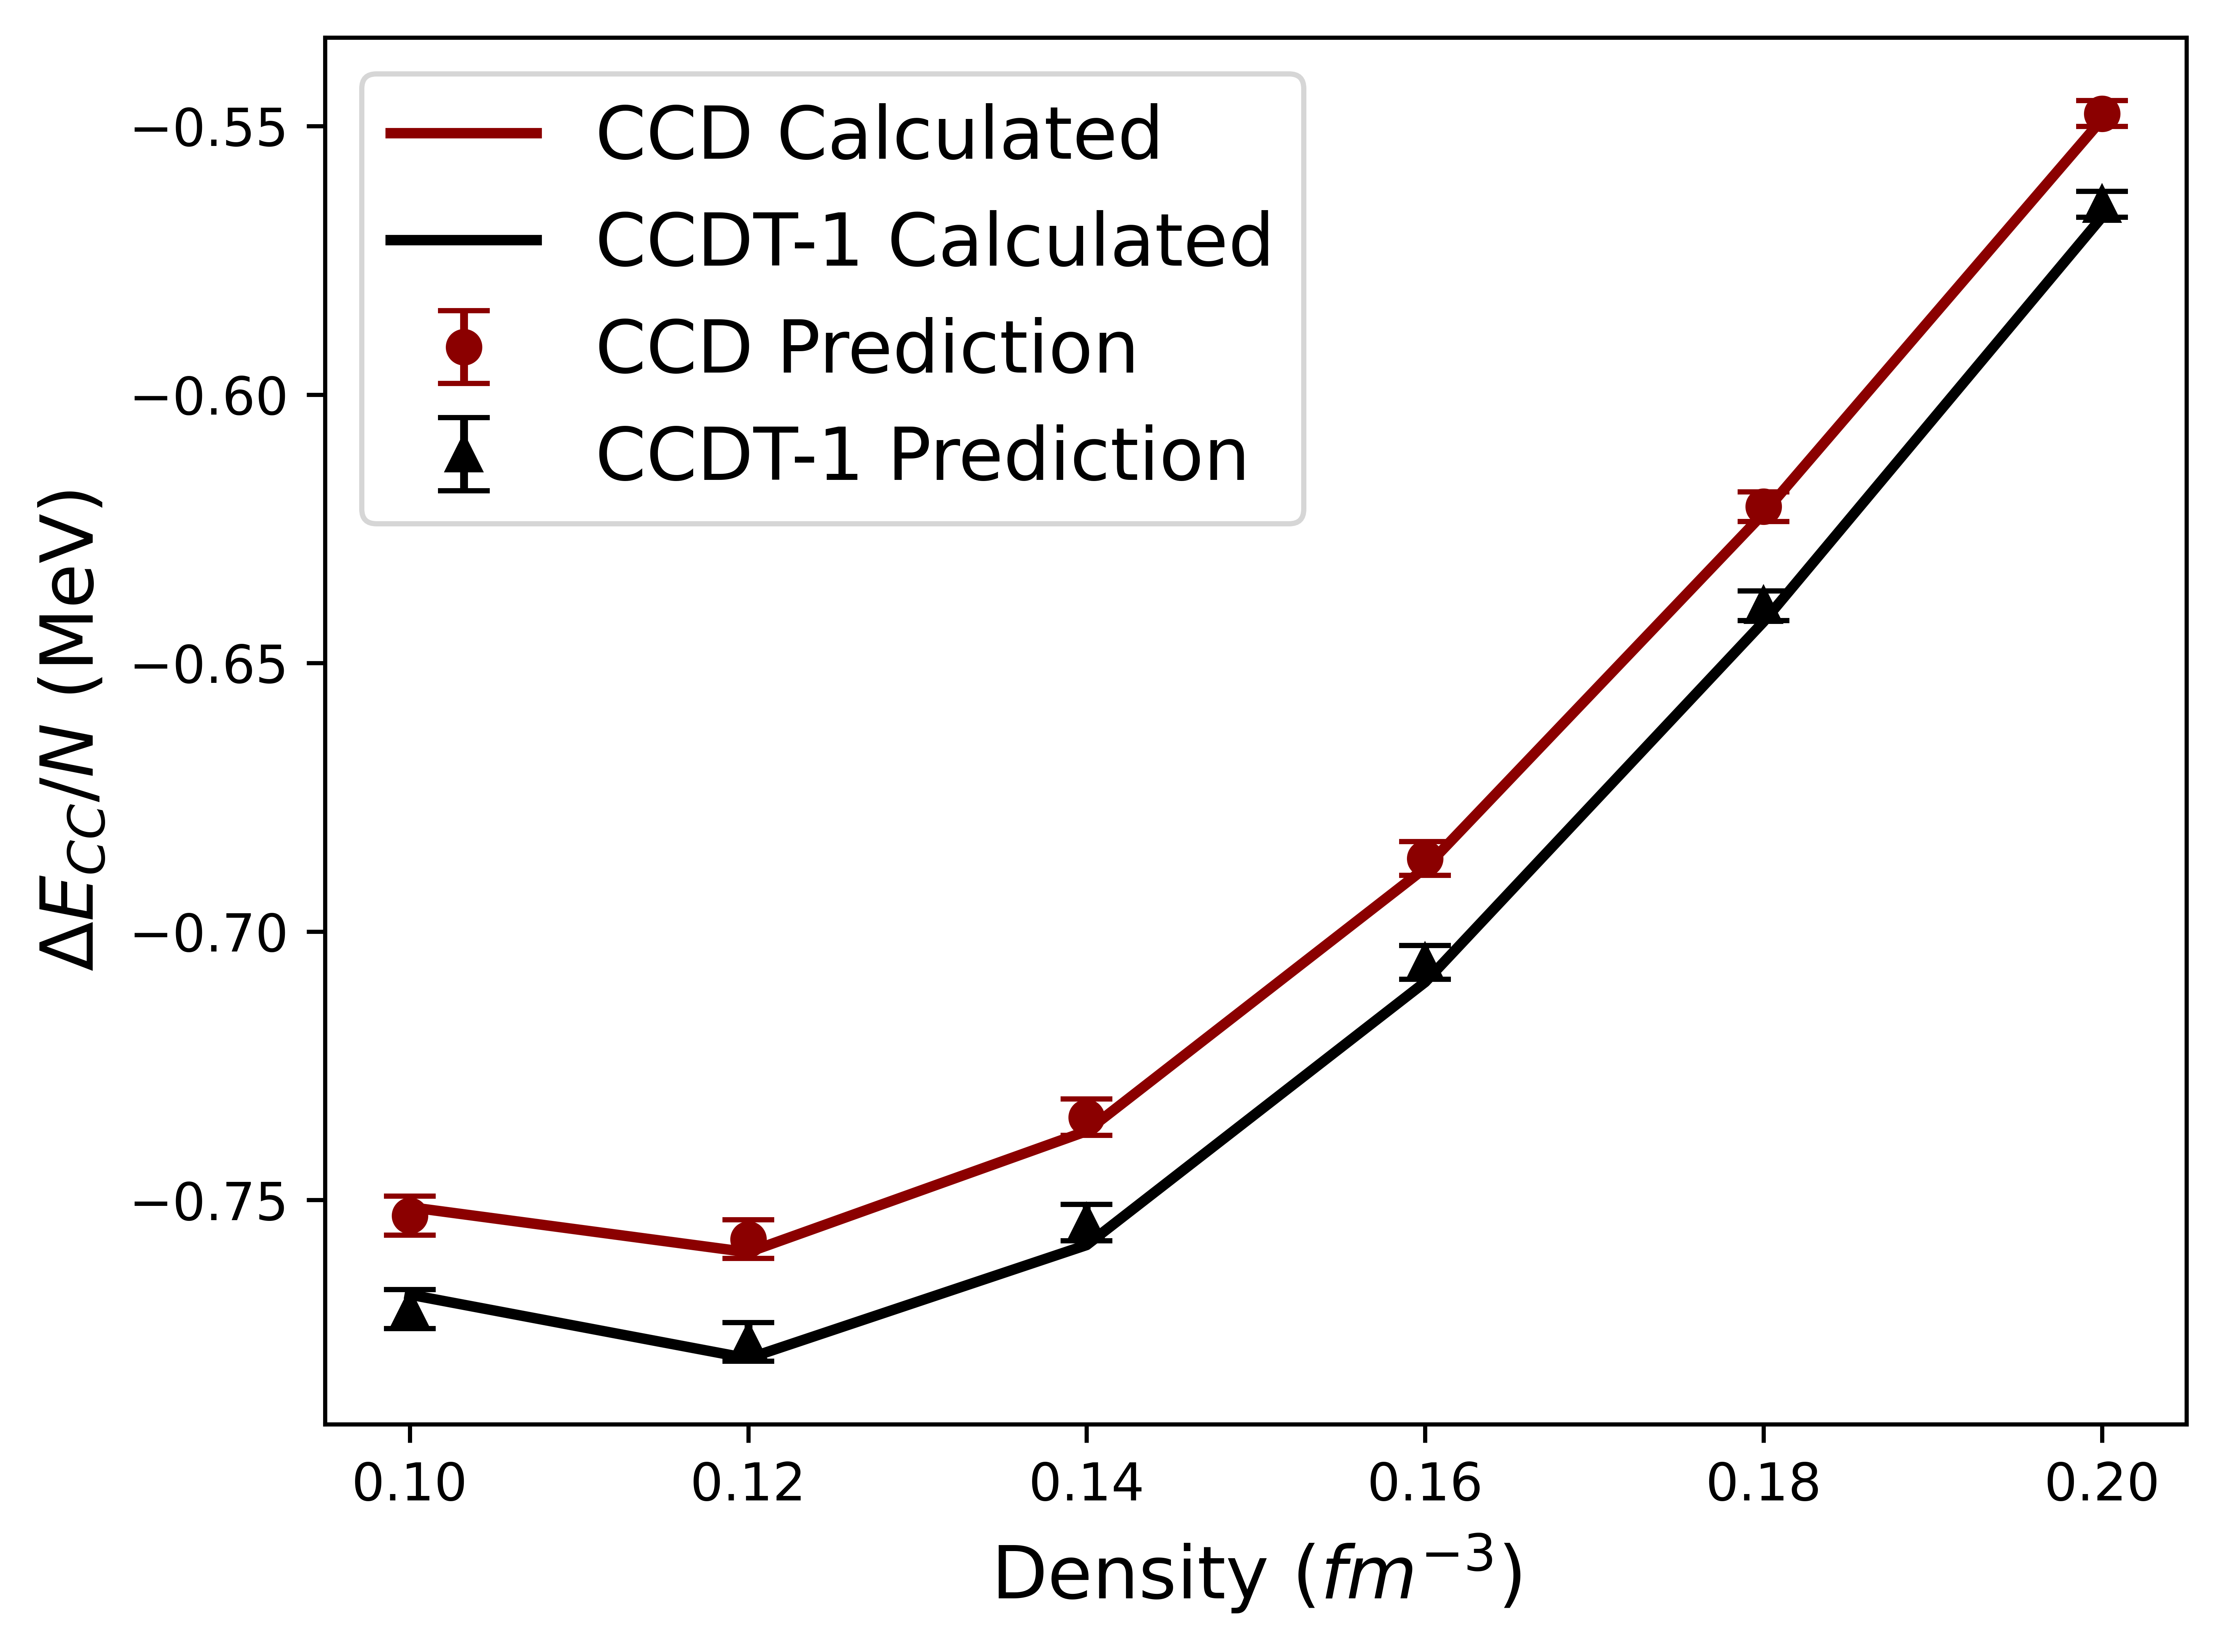
\includegraphics{Images/Chapter7/ORNL/ccdt1_nuclear_neutron_matter.png}
    \caption{CCD (red) versus CCDT-1 (black) correlation energies for a pure neutron matter system with 66 neutrons and chiral potentials. The converged correlation energies from full calculations are shown with solid lines, and the points represent the machine-learning predictions. The machine learning prediction is shown with the uncertainties from the Gaussian process algorithm.}
    \label{fig:ccd_and_ccddt1}
\end{figure}

        As a final set of calculations with pure neutron matter, we can look at performing CC calculations using the CCD(T) approximation.

%% CCD(T) DATA
First, let us compare the correlation energies of a PNM system for densities around nuclear density calculated using CCD, CCDT-1, and CCD(T).  It has already been shown that CCD and CCDT-1 give significantly different values for the correlation energies. Still, we want to ensure a significant difference between these two data sets and the CCD(T) energies. Fig. \ref{fig:compare_pnm_all_no_sre} shows the fully converged correlation energies for a PNM system calculated with the three CC approximations.  The CCD and CCD(T) were performed at M = 1,478, and the CCDT-1 calculations were performed at M = 514.  It does appear that the three methods give significantly different answers, so it will be an exciting test for the SRE method to compare its performance on all three methods.

\begin{figure}
    \centering
    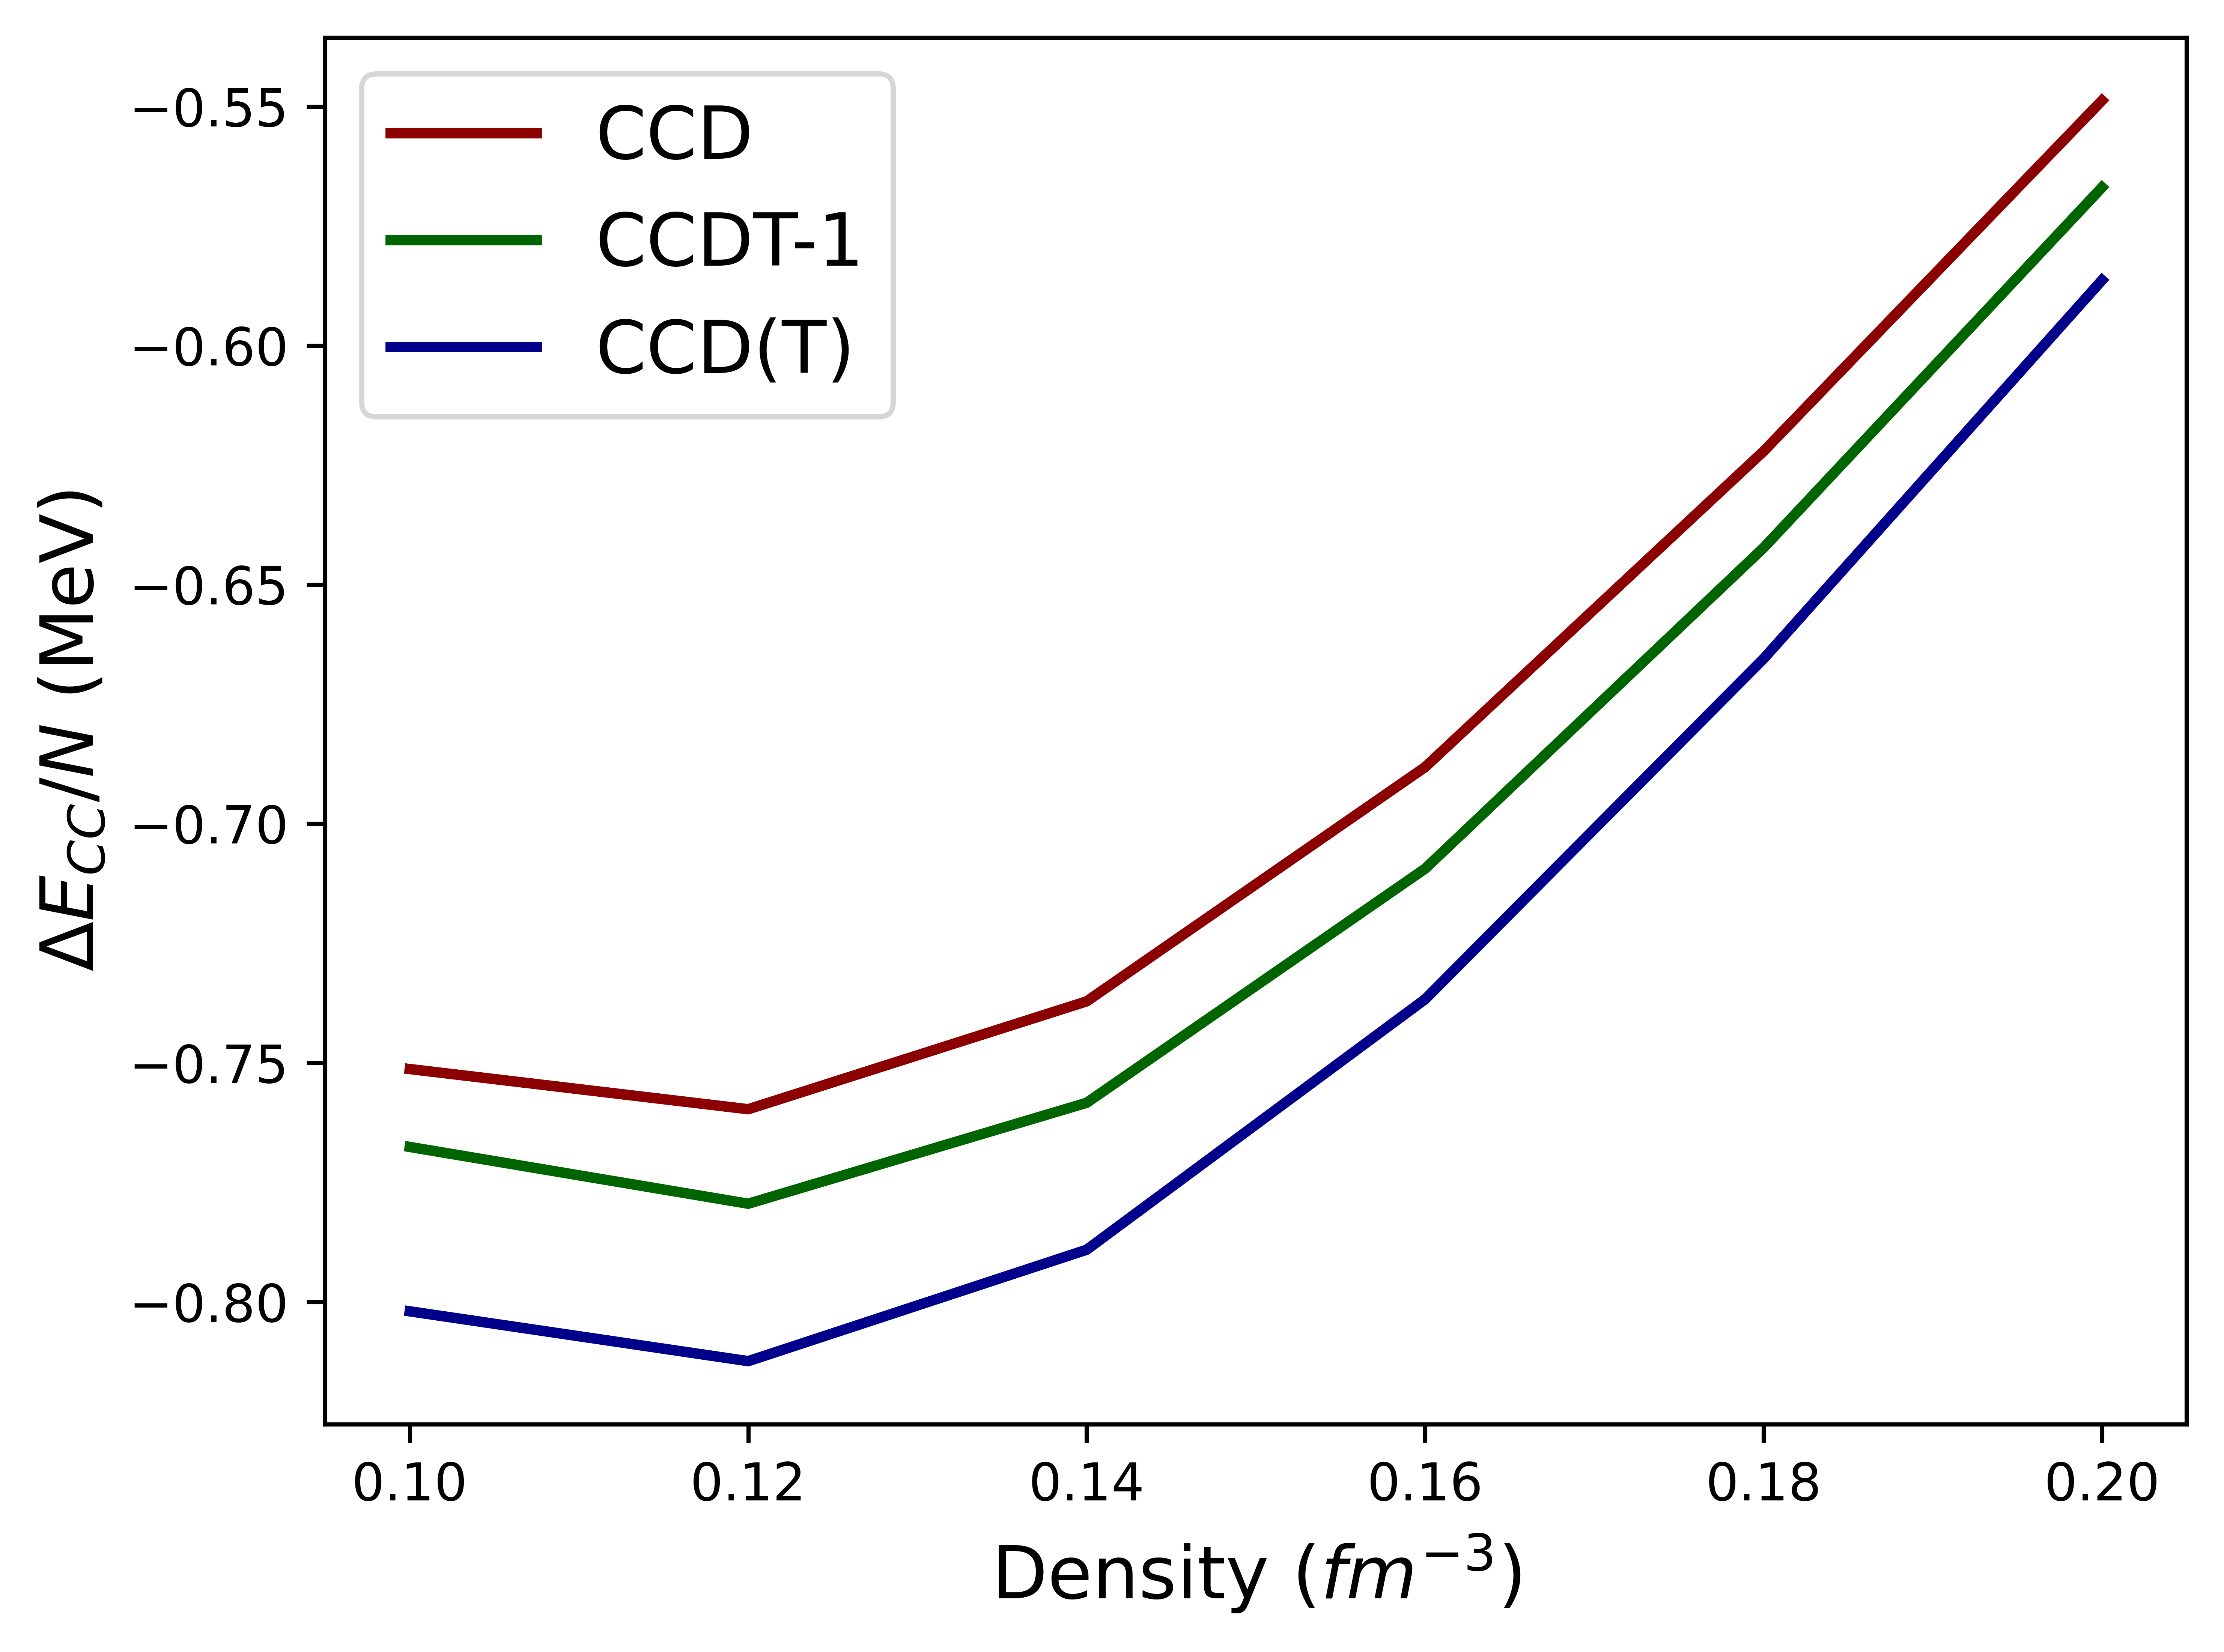
\includegraphics[scale=0.75]{Images/Chapter8/pnm_all_sre.png}
    \caption{Correlation energies of PNM calculated with CCD (red), CCDT-1 (green), and CCD(T) (blue) for densities around nuclear density.}
    \label{fig:compare_pnm_all_no_sre}
\end{figure}

Now, we can compare the run times of each method when applied to PNM.  The expected run time of a CCD calculation is an iterative $O(M^6)$, and the expected run time of a CCDT-1 calculation is an iterative $O(M^7)$.  In comparison, the expected run time of a CCD(T) calculation falls in between these two with an iterative $O(M^6)$ followed by a non-iterative step of $O(M^7)$.  And in fact, that is what we see in Fig. \ref{fig:all_times_pnm} where CCD(T) is faster than CCDT-1 but slower than CCD. Note that the times are reported here in node hours per GHz.  The CCD(T) calculations for PNM were performed on Oak Ridge National Laboratory's Andes supercomputer on Andes processors, which have a clock speed of 3.0 GHz and use 64 MPI nodes.  Just as we defined a node hour as the total run time of a calculation multiplied by the number of MPI nodes in the calculations to compare the run times computed with different numbers of MPI nodes, here we define node hours per GHz (node hours divided by the clock speed of the processors) to compare results which have been performed on different supercomputers. 

\begin{figure}
    \centering
    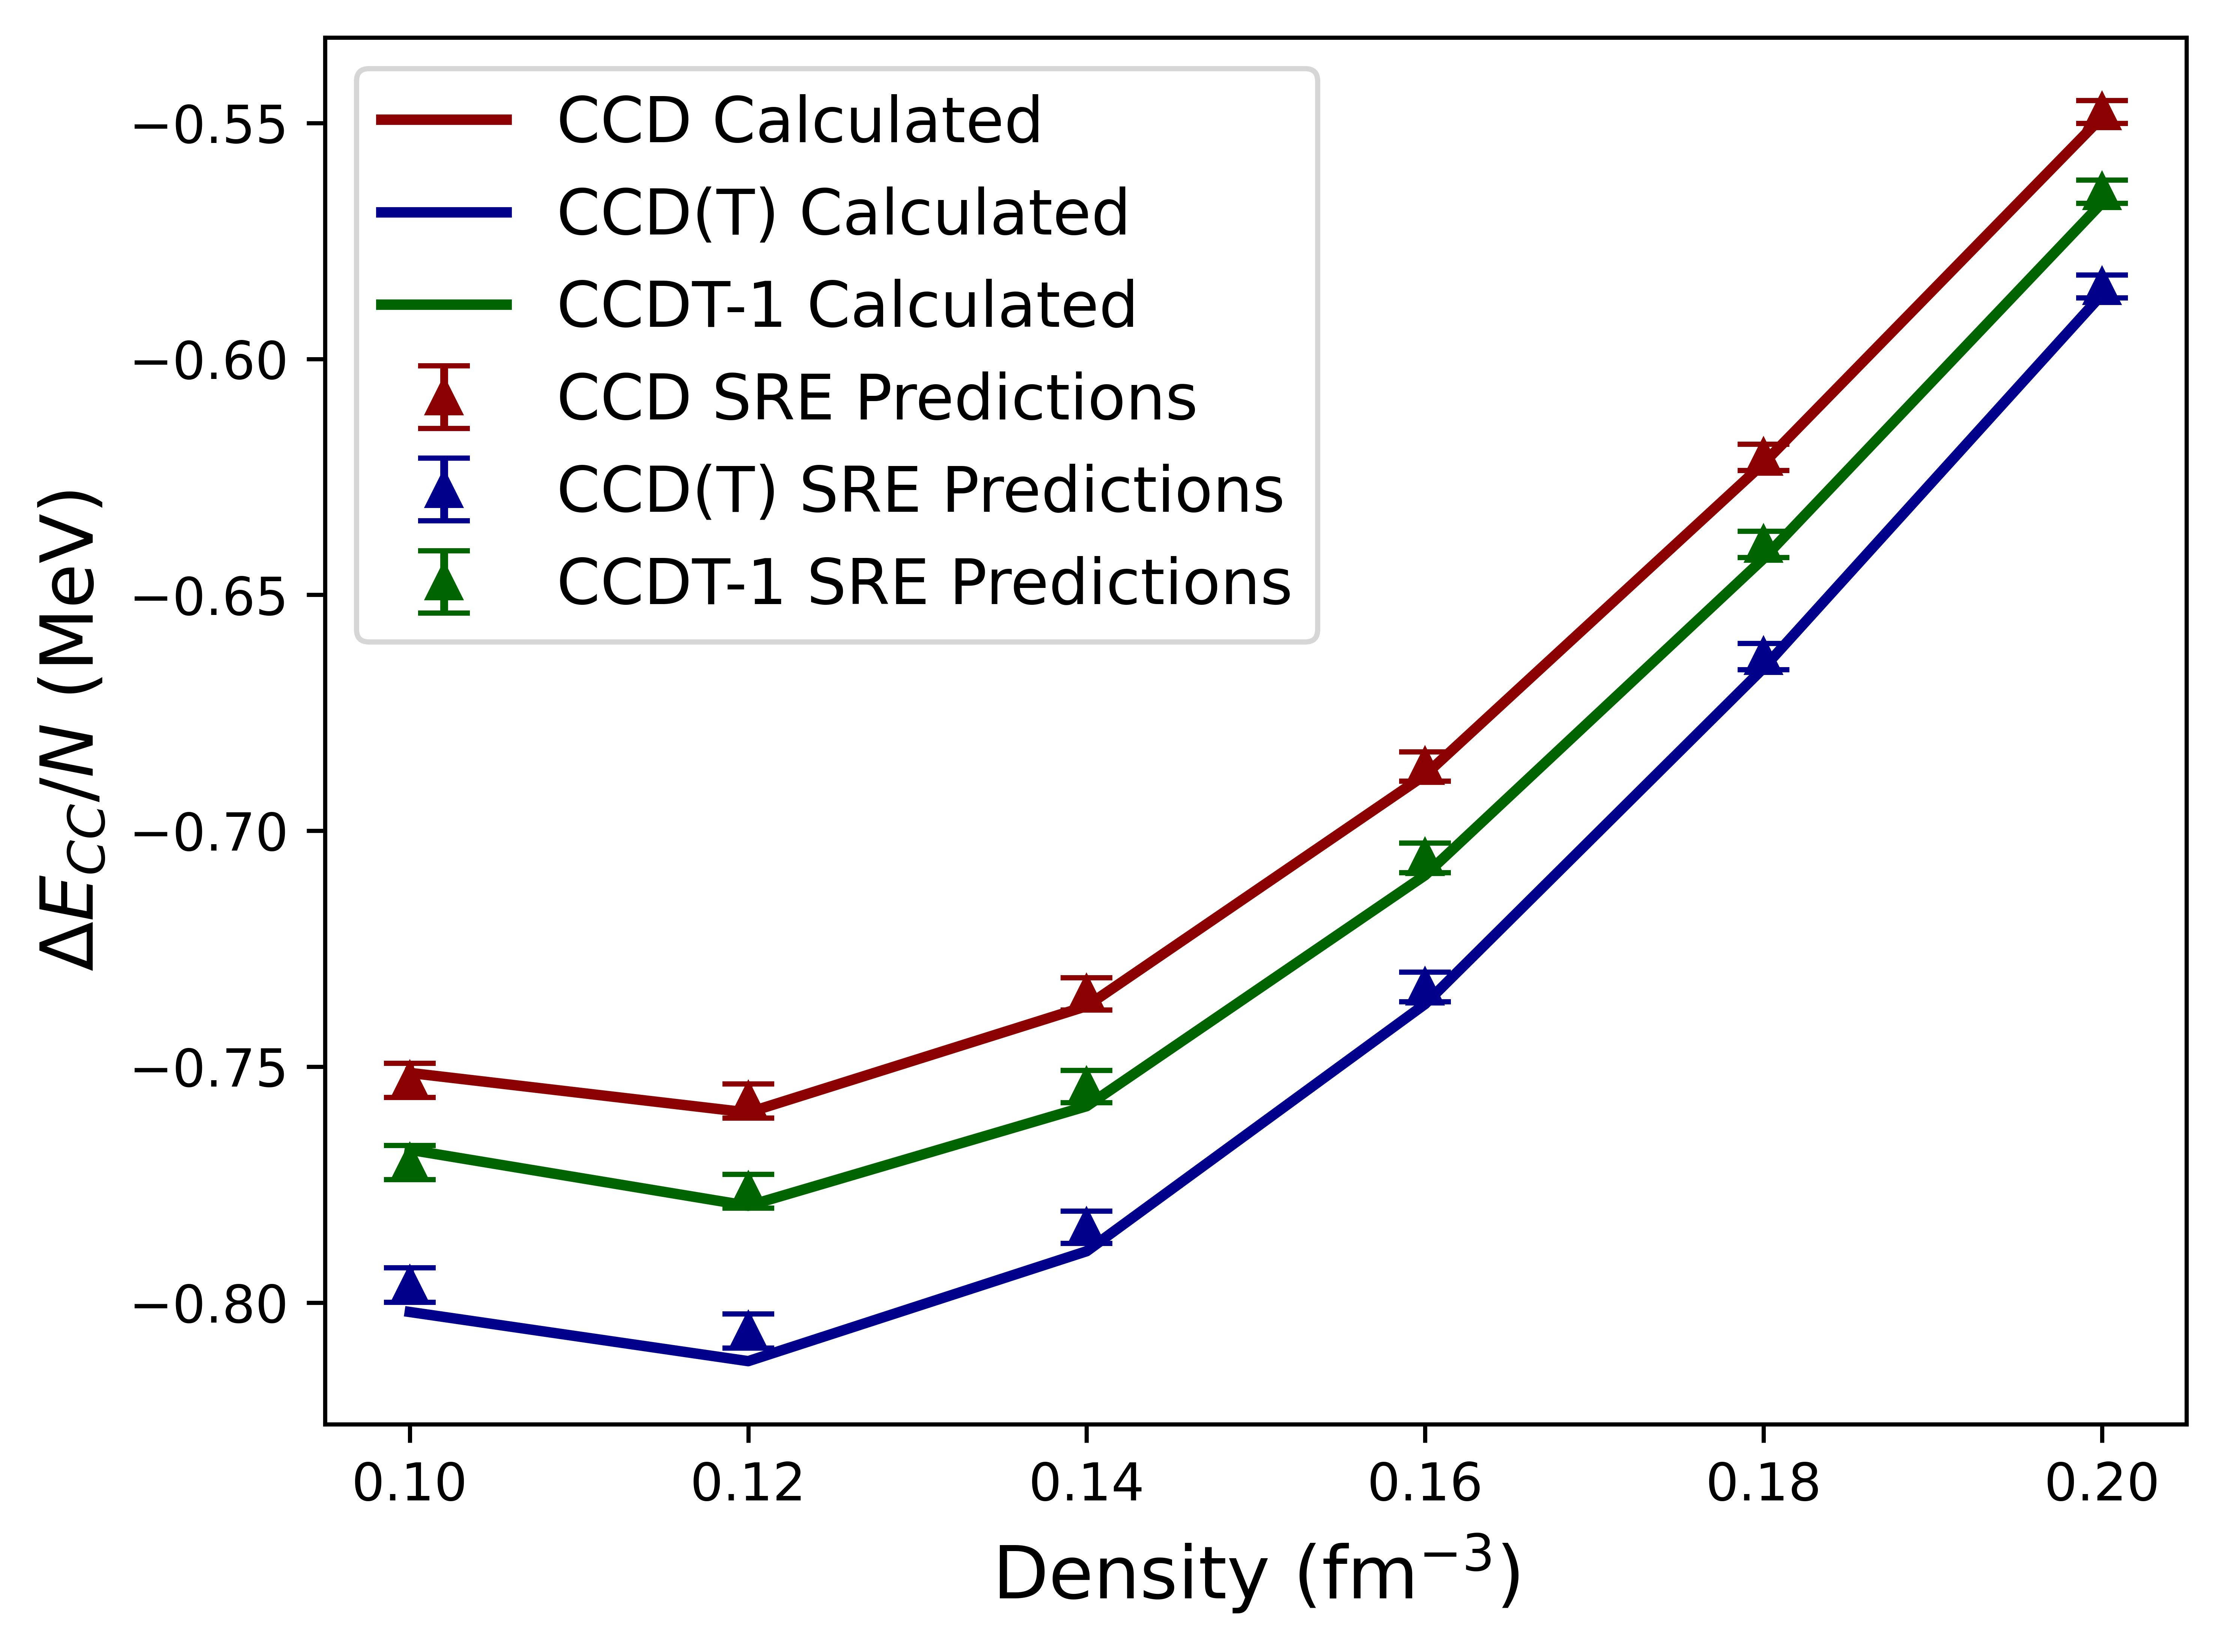
\includegraphics{Images/Chapter8/FinalReport6.png}
    \caption{The run time (in node hours per GHz) to calculate the correlation energies for a PNM system at d = 0.16fm$^{-3}$ calculated using CCD (red), CCDT-1 (green), and CCD(T) (blue) as a function of the number of single-particle states in the calculation.}
    \label{fig:all_times_pnm}
\end{figure}

Now we can apply the SRE method to attempt to predict the converged CCD(T) correlation energies for PNM.  We have used three training points, like with the other PNM and chiral potential extrapolations. Still, here we have moved the training data to slightly higher numbers of single-particle states (M = 186, 246, and 294) due to the slower convergence of the CCD(T) correlation energies with respect to the number of single-particle states.  We have kept the SRE sequence length as 1.  Fig. \ref{fig:sre_pnm_ccdt_pert} shows the results of performing this SRE analysis with the full CCD(T) correlation energy calculations performed at M = 1,478 shown with the solid line and the SRE predictions with the triangular markers.  Here the average percent error between the two data sets is 0.54$\%$.  Furthermore, the time needed to perform the six CCD(T) calculations at M = 1,478 shown in Fig. \ref{fig:sre_pnm_ccdt_pert} took 594.15 node hours, but the time needed to generate the SRE training data was only 32.16 node hours.  This leads to a time savings of 561.99 node hours or 23.41 \textit{node days}.

\begin{figure}
    \centering
    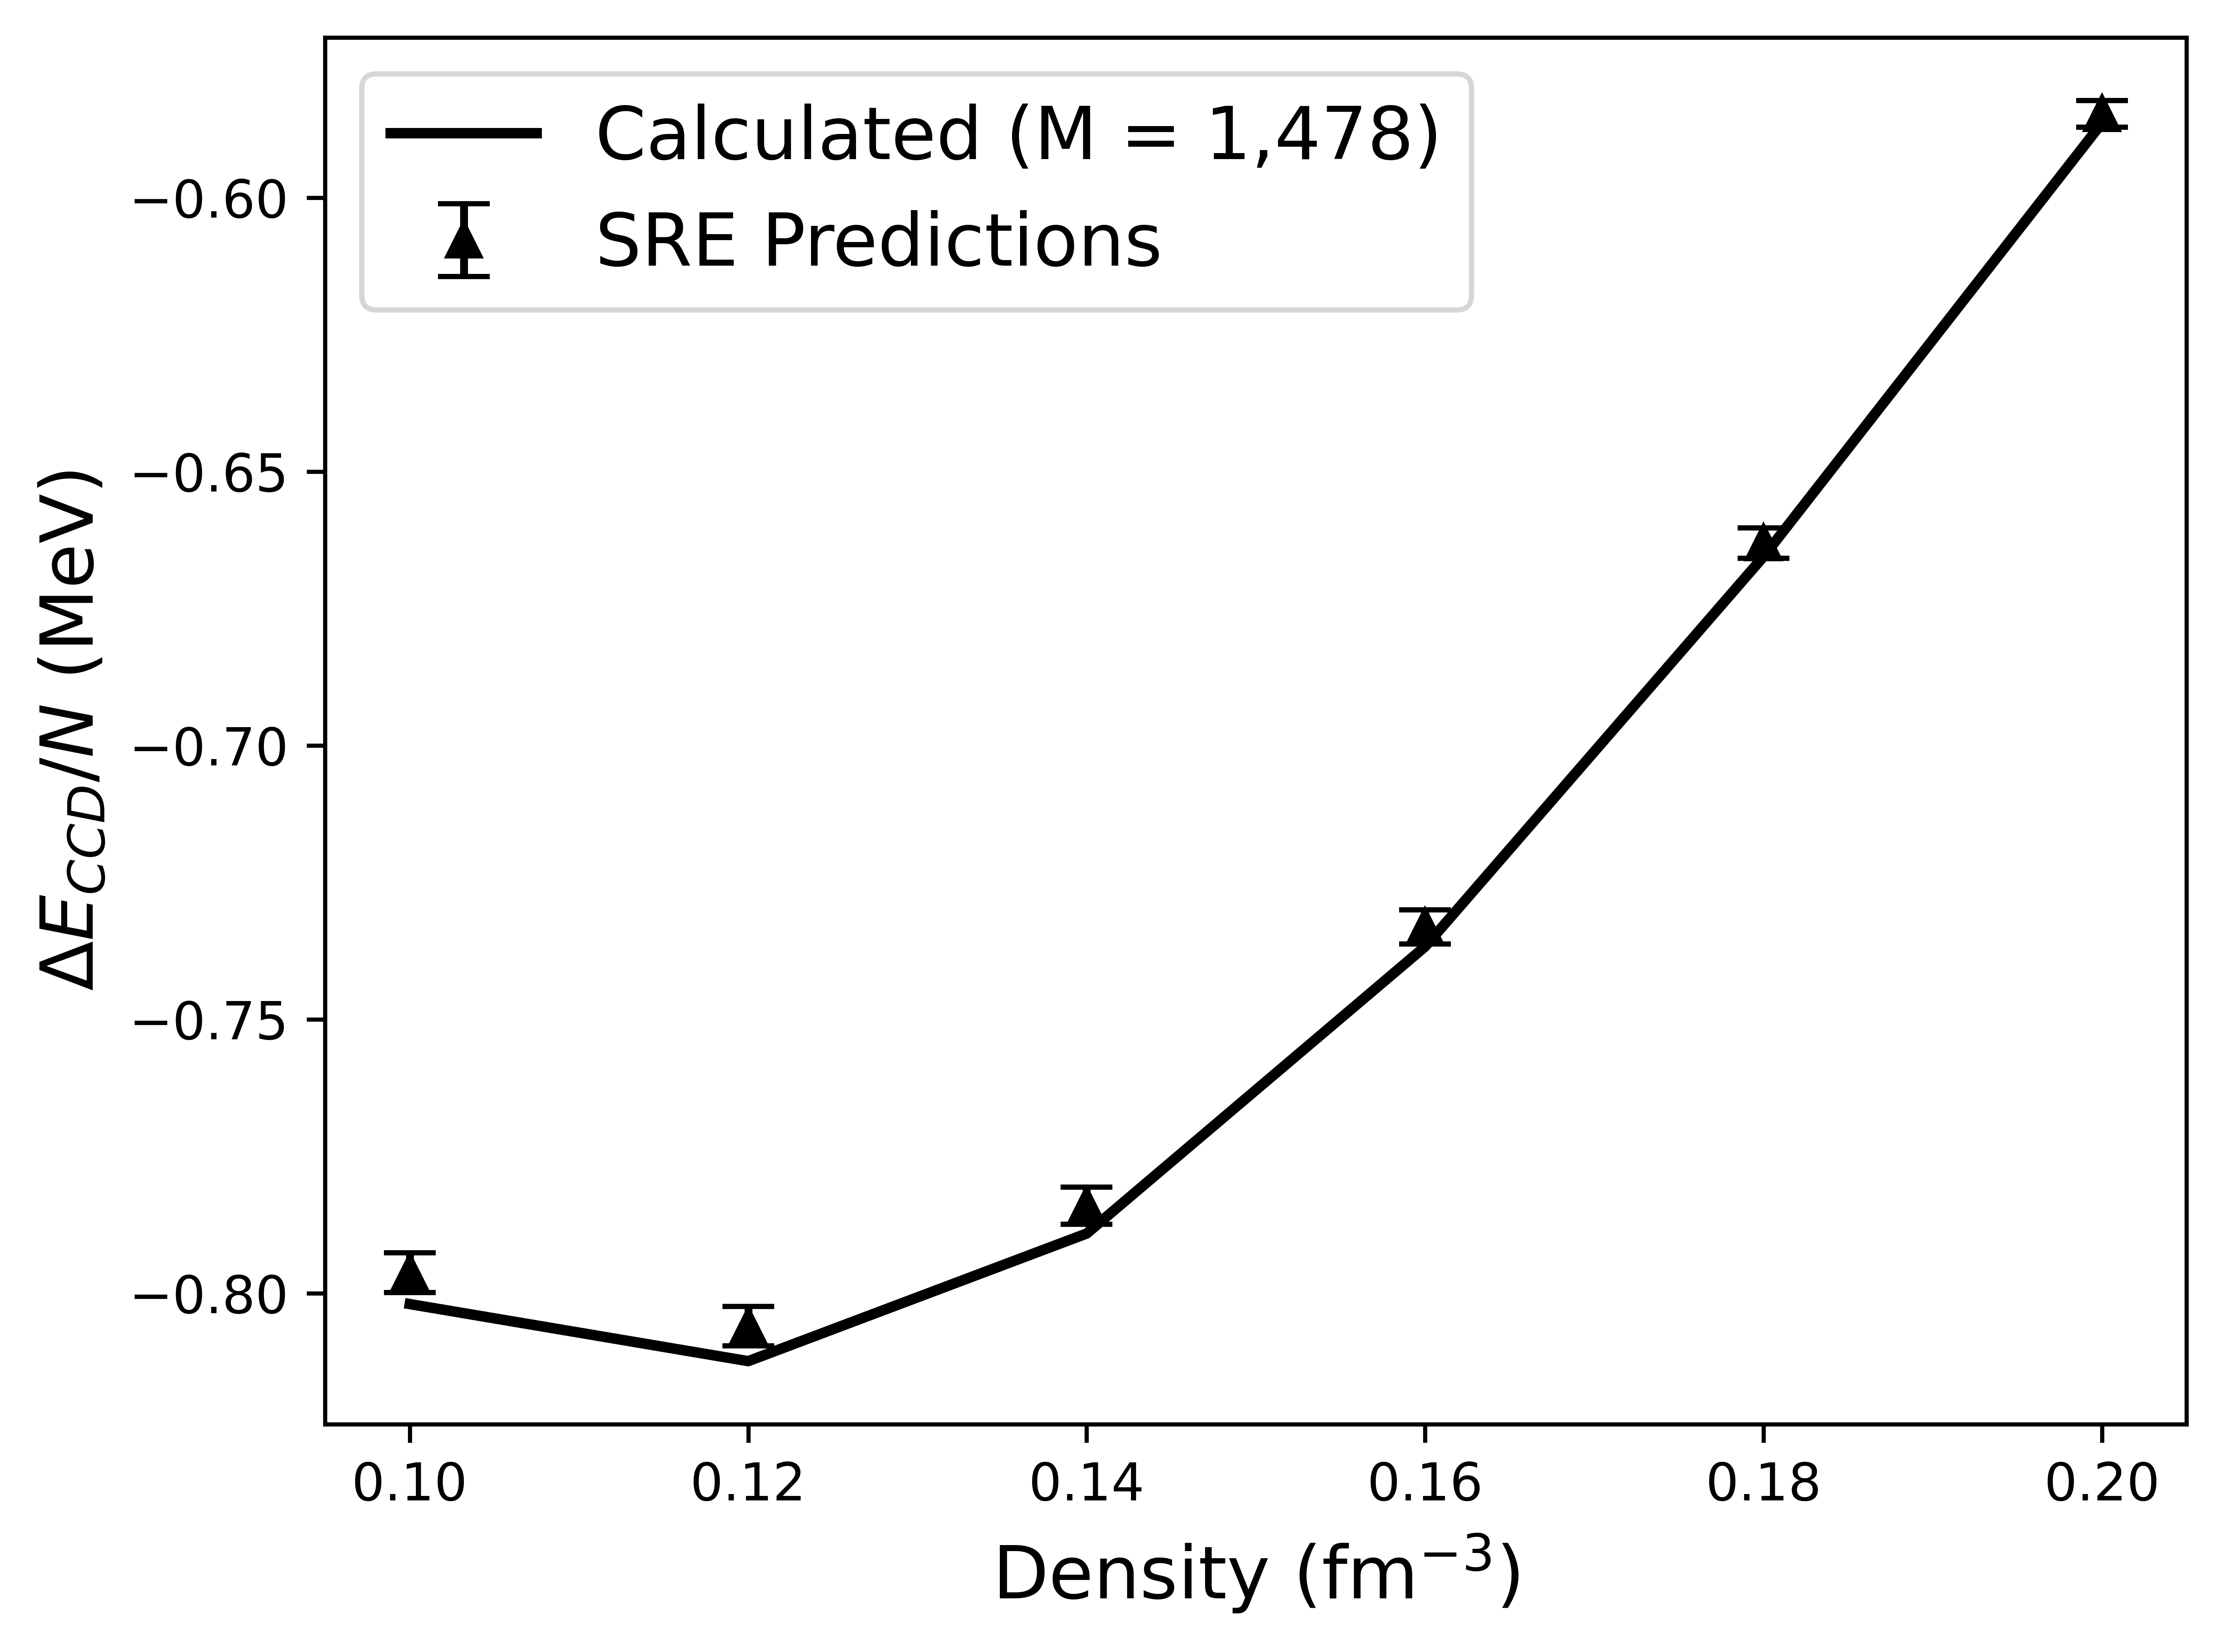
\includegraphics{Images/Chapter8/FinalReport4a.png}
    \caption{The CCD(T) correlation energies for PNM for densities around nuclear density were calculated at M = 1,478 (solid line) and predicted with the SRE method (triangular markers).  The uncertainties from the Gaussian processes algorithm are shown with error bars on the markers.}
    \label{fig:sre_pnm_ccdt_pert}
\end{figure}


Finally, we are in a position to compare the SRE predictions for CC calculations of PNM using CCD (red), CCDT-1 (green), and CCD(T) (blue), as seen in Fig \ref{fig:compare_pnm_all_sre}.  For all three CC methods, the complete calculations are shown with solid lines. The SRE predictions are shown with triangular markers with error bars, with the error bars representing the uncertainties from the Gaussian processes algorithm. For all three data sets, the SRE method appears to provide a good match for all the correlation energies across all the densities shown.  The average percent error of this figure is 0.42$\%$.  Furthermore, the entire time saved u
using the SRE method to predict the converged correlation energies rather than fully calculating them is 796.89 node hours or 33.20 \textit{node days}.  Therefore, in calculating just 18 points for the PNM system, we save over a month of computational time using the SRE method. 

\begin{figure}
    \centering
    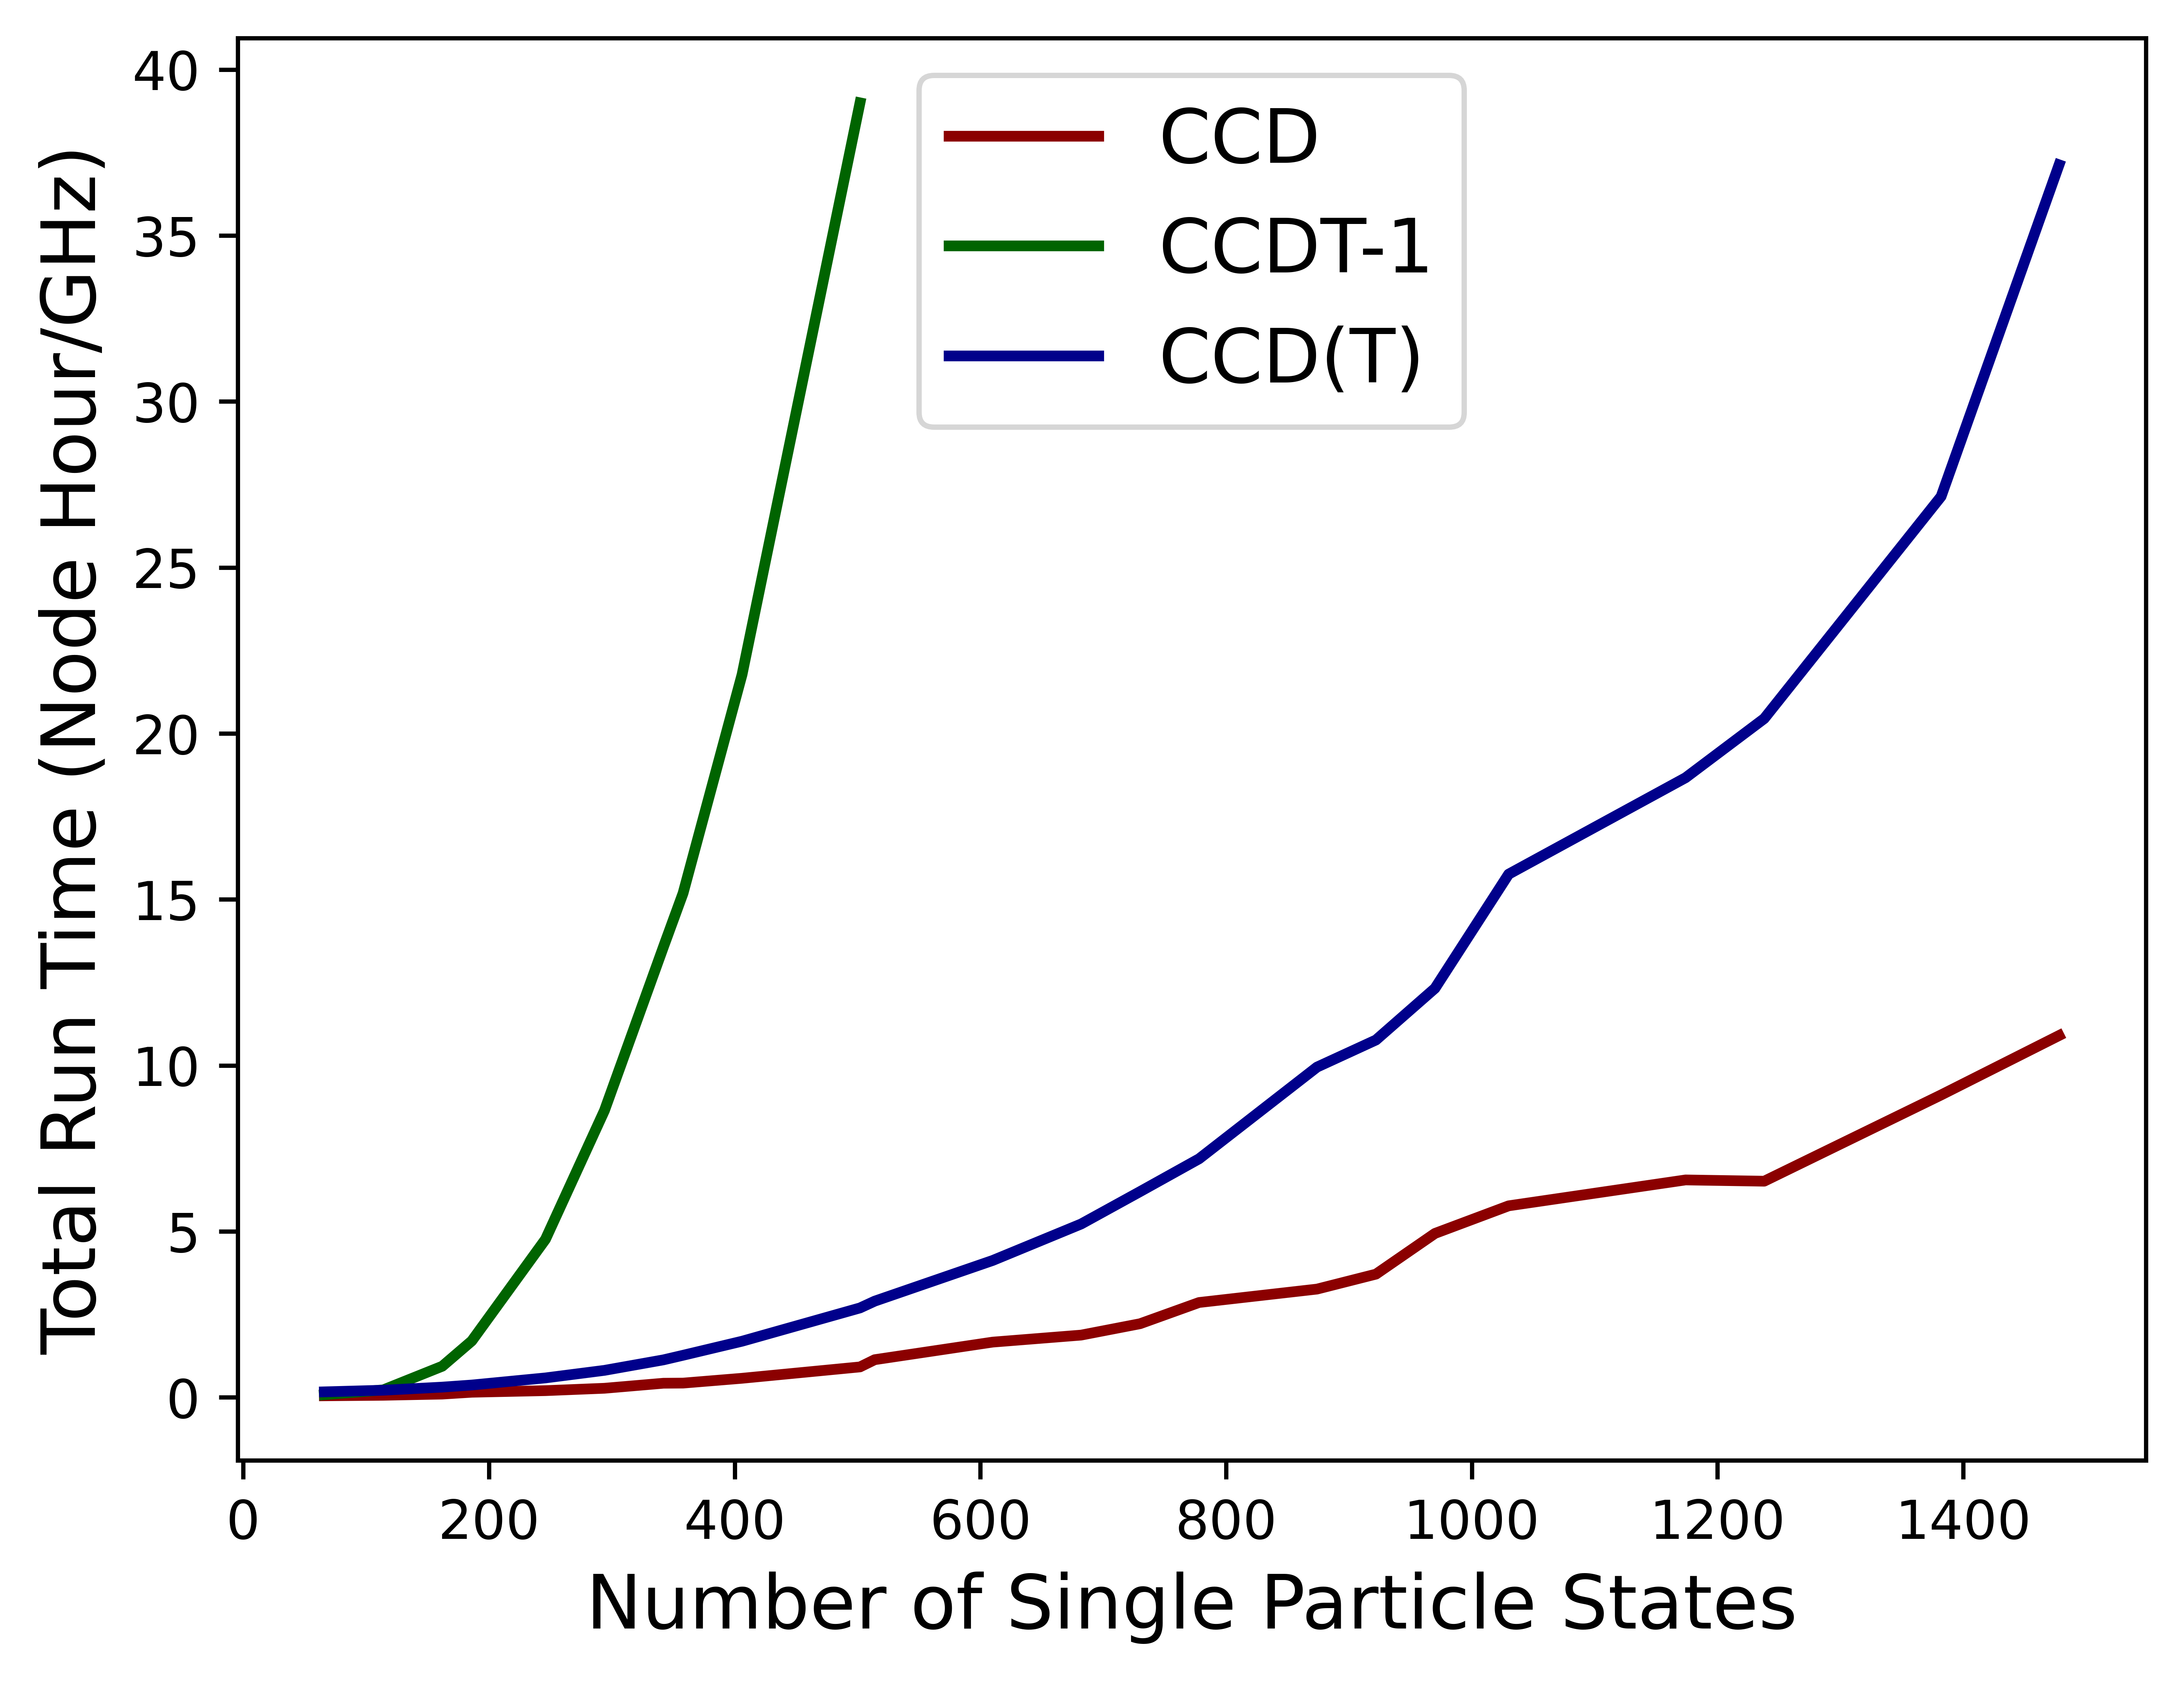
\includegraphics{Images/Chapter8/FinalReport7.png}
    \caption{The correlation energies for PNM were calculated using CCD (red), CCDT-1 (green), and CCD(T) (blue).  The fully converged calculations are shown with the solid lines, and the SRE predictions are shown with the triangular markers.}
    \label{fig:compare_pnm_all_sre}
\end{figure}

In this section, we have performed coupled cluster calculations of pure neutron matter using two different models of nuclear interaction and three different levels of coupled cluster approximations.  However, it is essential to note that the main point of this section is not to compare the effects of different coupled cluster calculations and interactions, though we have done this.  Instead, the main point of this section is to determine the performance of the SRE methods on different types of coupled cluster calculations.  As we have seen throughout this section, the SRE method can accurately extrapolate to the converged correlation energy of the pure neutron matter system, regardless of the combination of nuclear interaction and coupled cluster approximation used. Furthermore, over a month of computational time is saved in this section by using the SRE method with no loss of relevant accuracy. Finally, it is essential to note that even though we are using machine learning, the training data sets we have used range from 3 - 10 data points. These are some of the smallest training data sets found in the literature for machine learning applications in the physical sciences and emphasize an essential feature of the SRE method.  That being that the SRE method can make very accurate extrapolations using very little training data..

    %%%%%%%%%%%%%%%%%%%%%%%%%%%%%%
    %% Symmetric Nuclear Matter
    %%%%%%%%%%%%%%%%%%%%%%%%%%%%%%
    \section{Symmetric Nuclear Matter}
        \subsection{Coupled Cluster Doubles with Realistic Nuclear Interactions}

Now, we can move on from analyzing pure neutron matter and instead turn our attention to symmetric nuclear matter (SNM), which comprises an equivalent number of protons and neutrons. We will continue to use the chiral NNLO potentials. Here all SNM systems will be calculated using 132 nucleons (66 protons and 66 neutrons) since these results will be similar to the energies at the TDL \cite{Ref9}.   Furthermore, the immense computational costs of SNM calculations also prohibit studies and higher particle numbers. Compared to a PNM calculation, an SNM calculation will need to double the number of single-particle states to accommodate double the number of particles. It will need approximately three times the computational time and resources. However, it is essential to perform calculations of SNM in addition to PNM even at the higher computational costs because the addition of protons into the system causes different correlations in the system, leading to a correlation energy that converges slower with respect to the number of single-particle states. Thus SNM should be a more challenging system for the SRE method and will genuinely test its predictive abilities.
Additionally, as we think about moving towards calculations of finite nuclei in future works, accurate calculations of both PNM and SNM are essential for these studies. Fig. \ref{fig:pnm_and_snm} compares the CCD correlation energies per nucleon for PNM (red) and SNM (blue). We can see that the SNM correlation energies are significantly larger than the PNM ones.



\begin{figure}
    \centering
    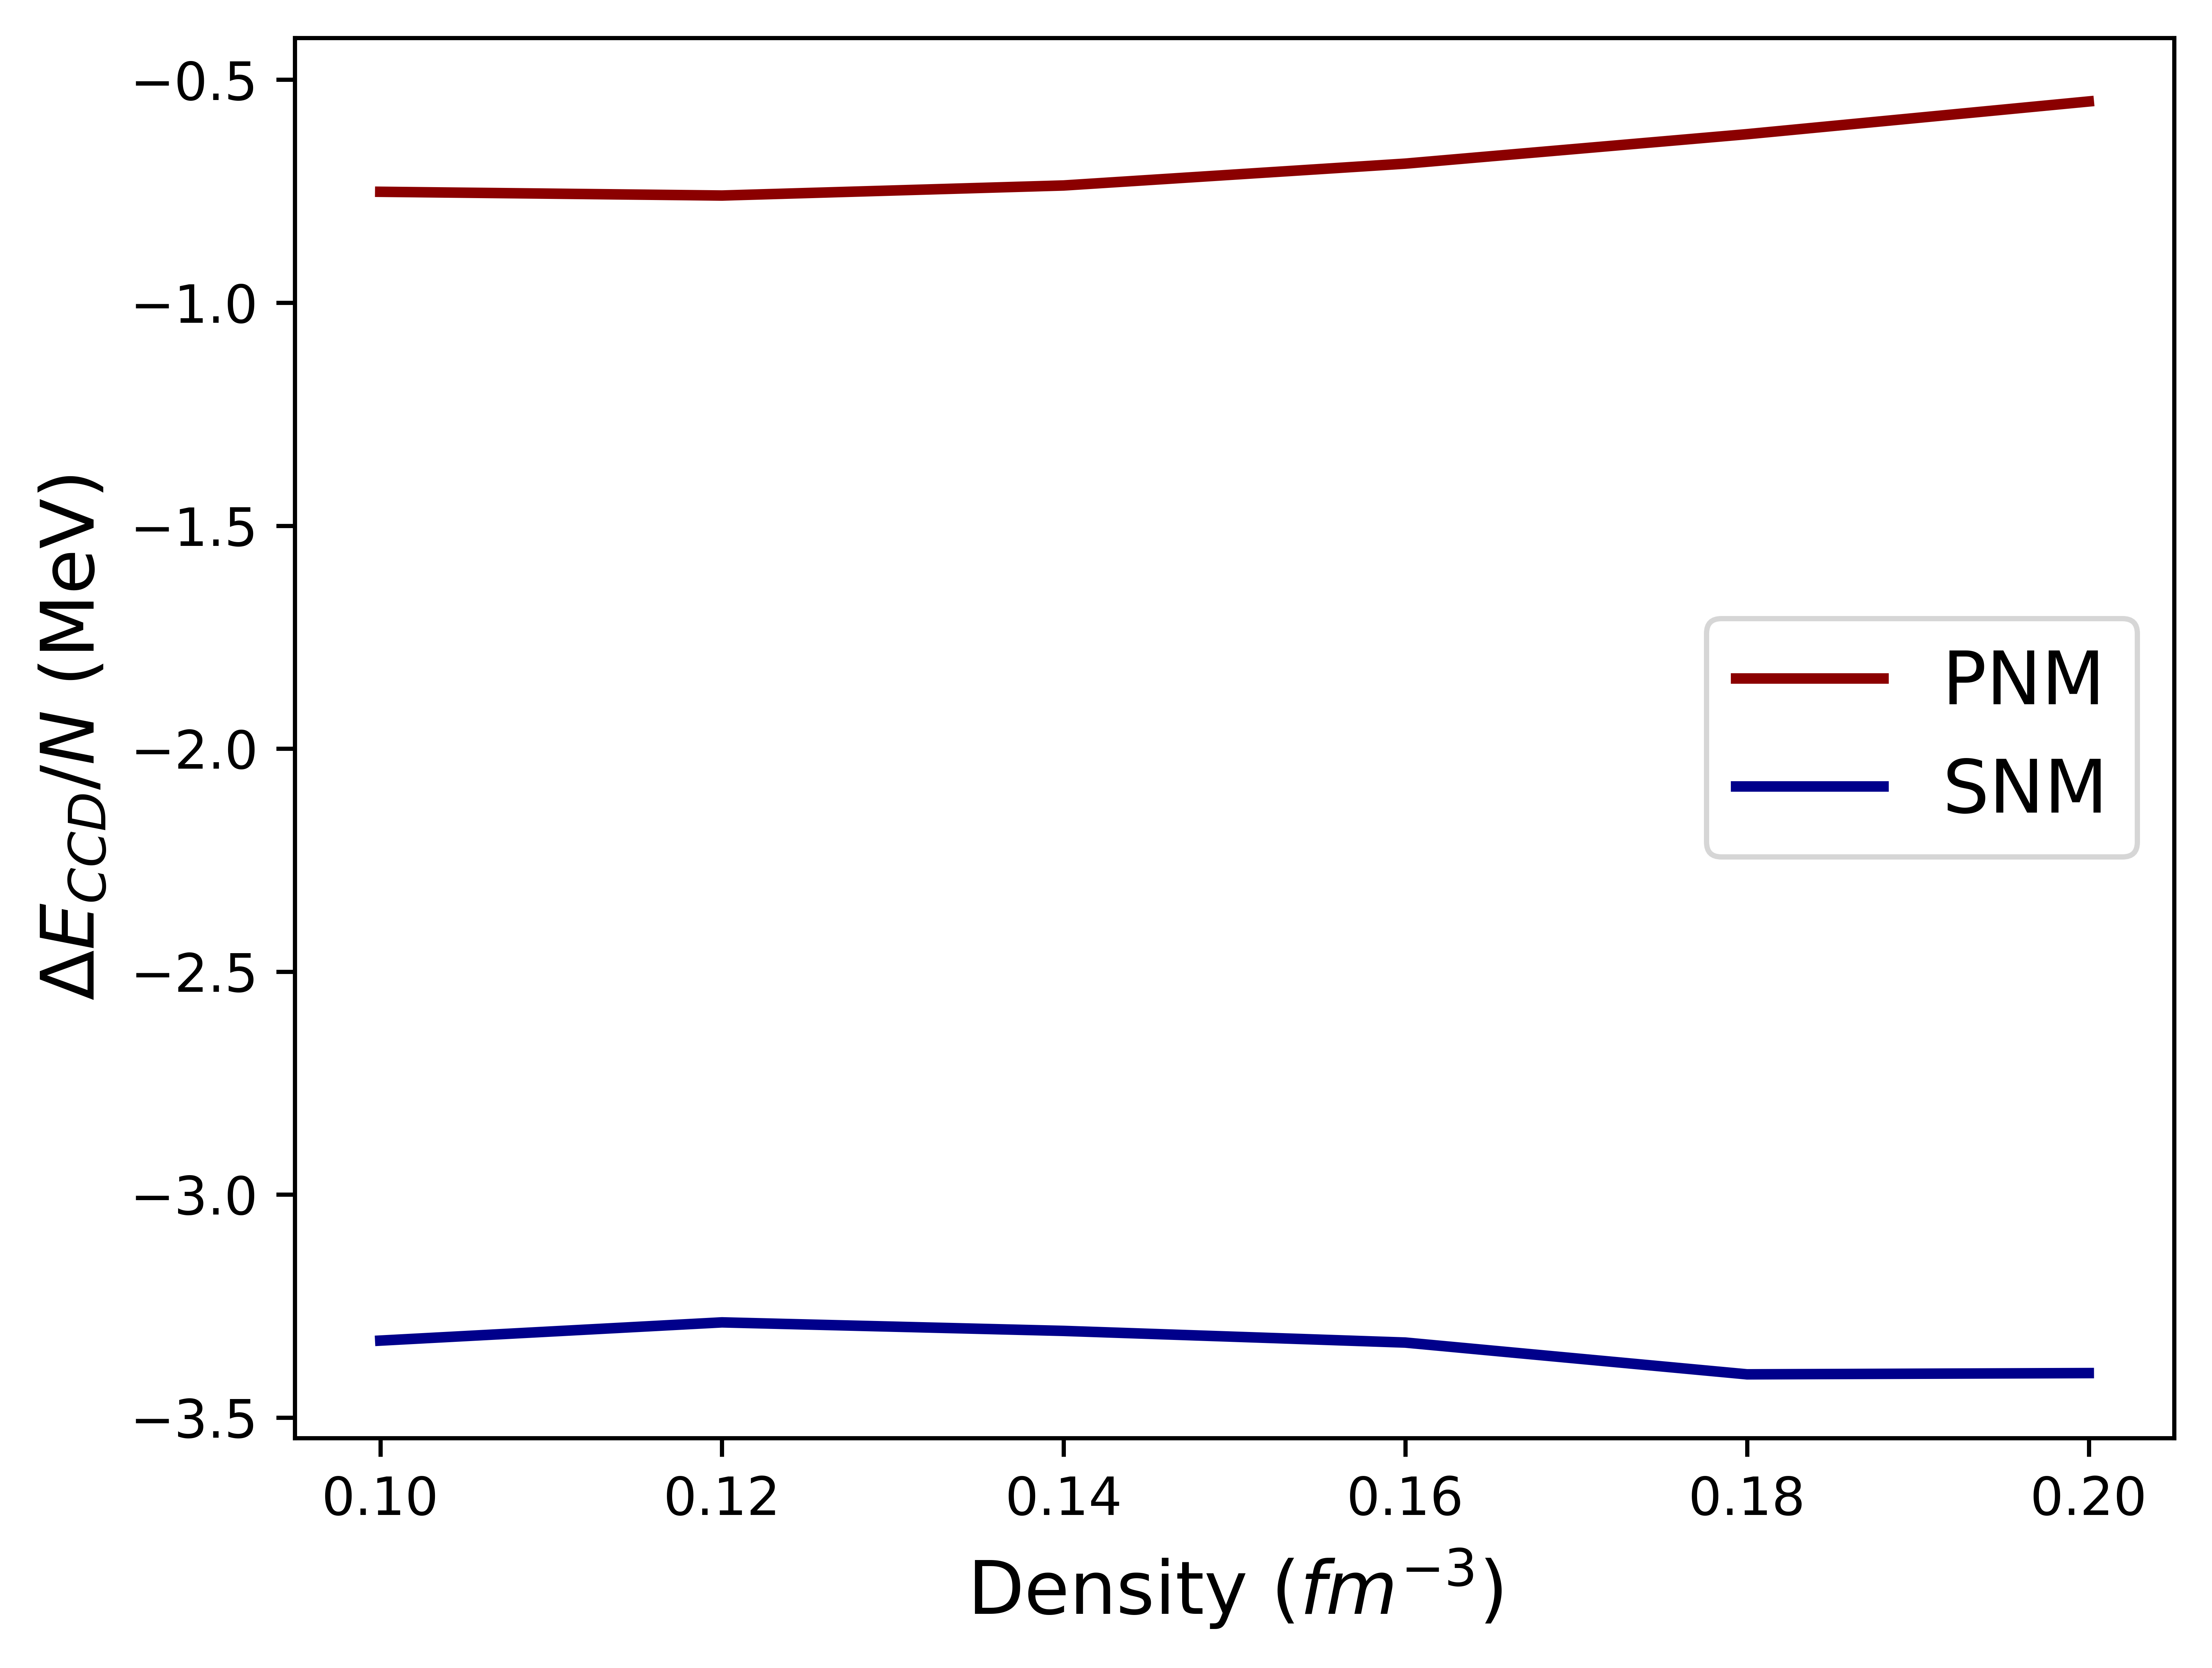
\includegraphics[scale=0.75]{Images/Chapter8/pnm_and_snm.png}
    \caption{The CCD correlation energies for PNM (red) and SNM (blue) for densities around nuclear matter and with a chiral NNLO potential.}
    \label{fig:pnm_and_snm}
\end{figure}

The CCD data set for SNM was generated using a supercomputer available through Michigan State University's Institute for Cyber-Enabled Research (ICER) using Intel Xeon processors, which have a clock speed of 2.4 GHz. For the MPI parallelization, 24 nodes were used. It takes, on average, 26.07 node hours to generate a converged CCD energy for a PNM system (at M = 1,478). However, since SNM is a more challenging case, and the number of single-particle states doubles, it takes, on average, 84.12 node hours to perform a converged CCD correlation energy calculation for SNM at M = 2,956. This means the computational resources needed for an SNM calculation are more significant than those needed for a PNM calculation by about a factor of three.

\begin{figure}
    \centering
    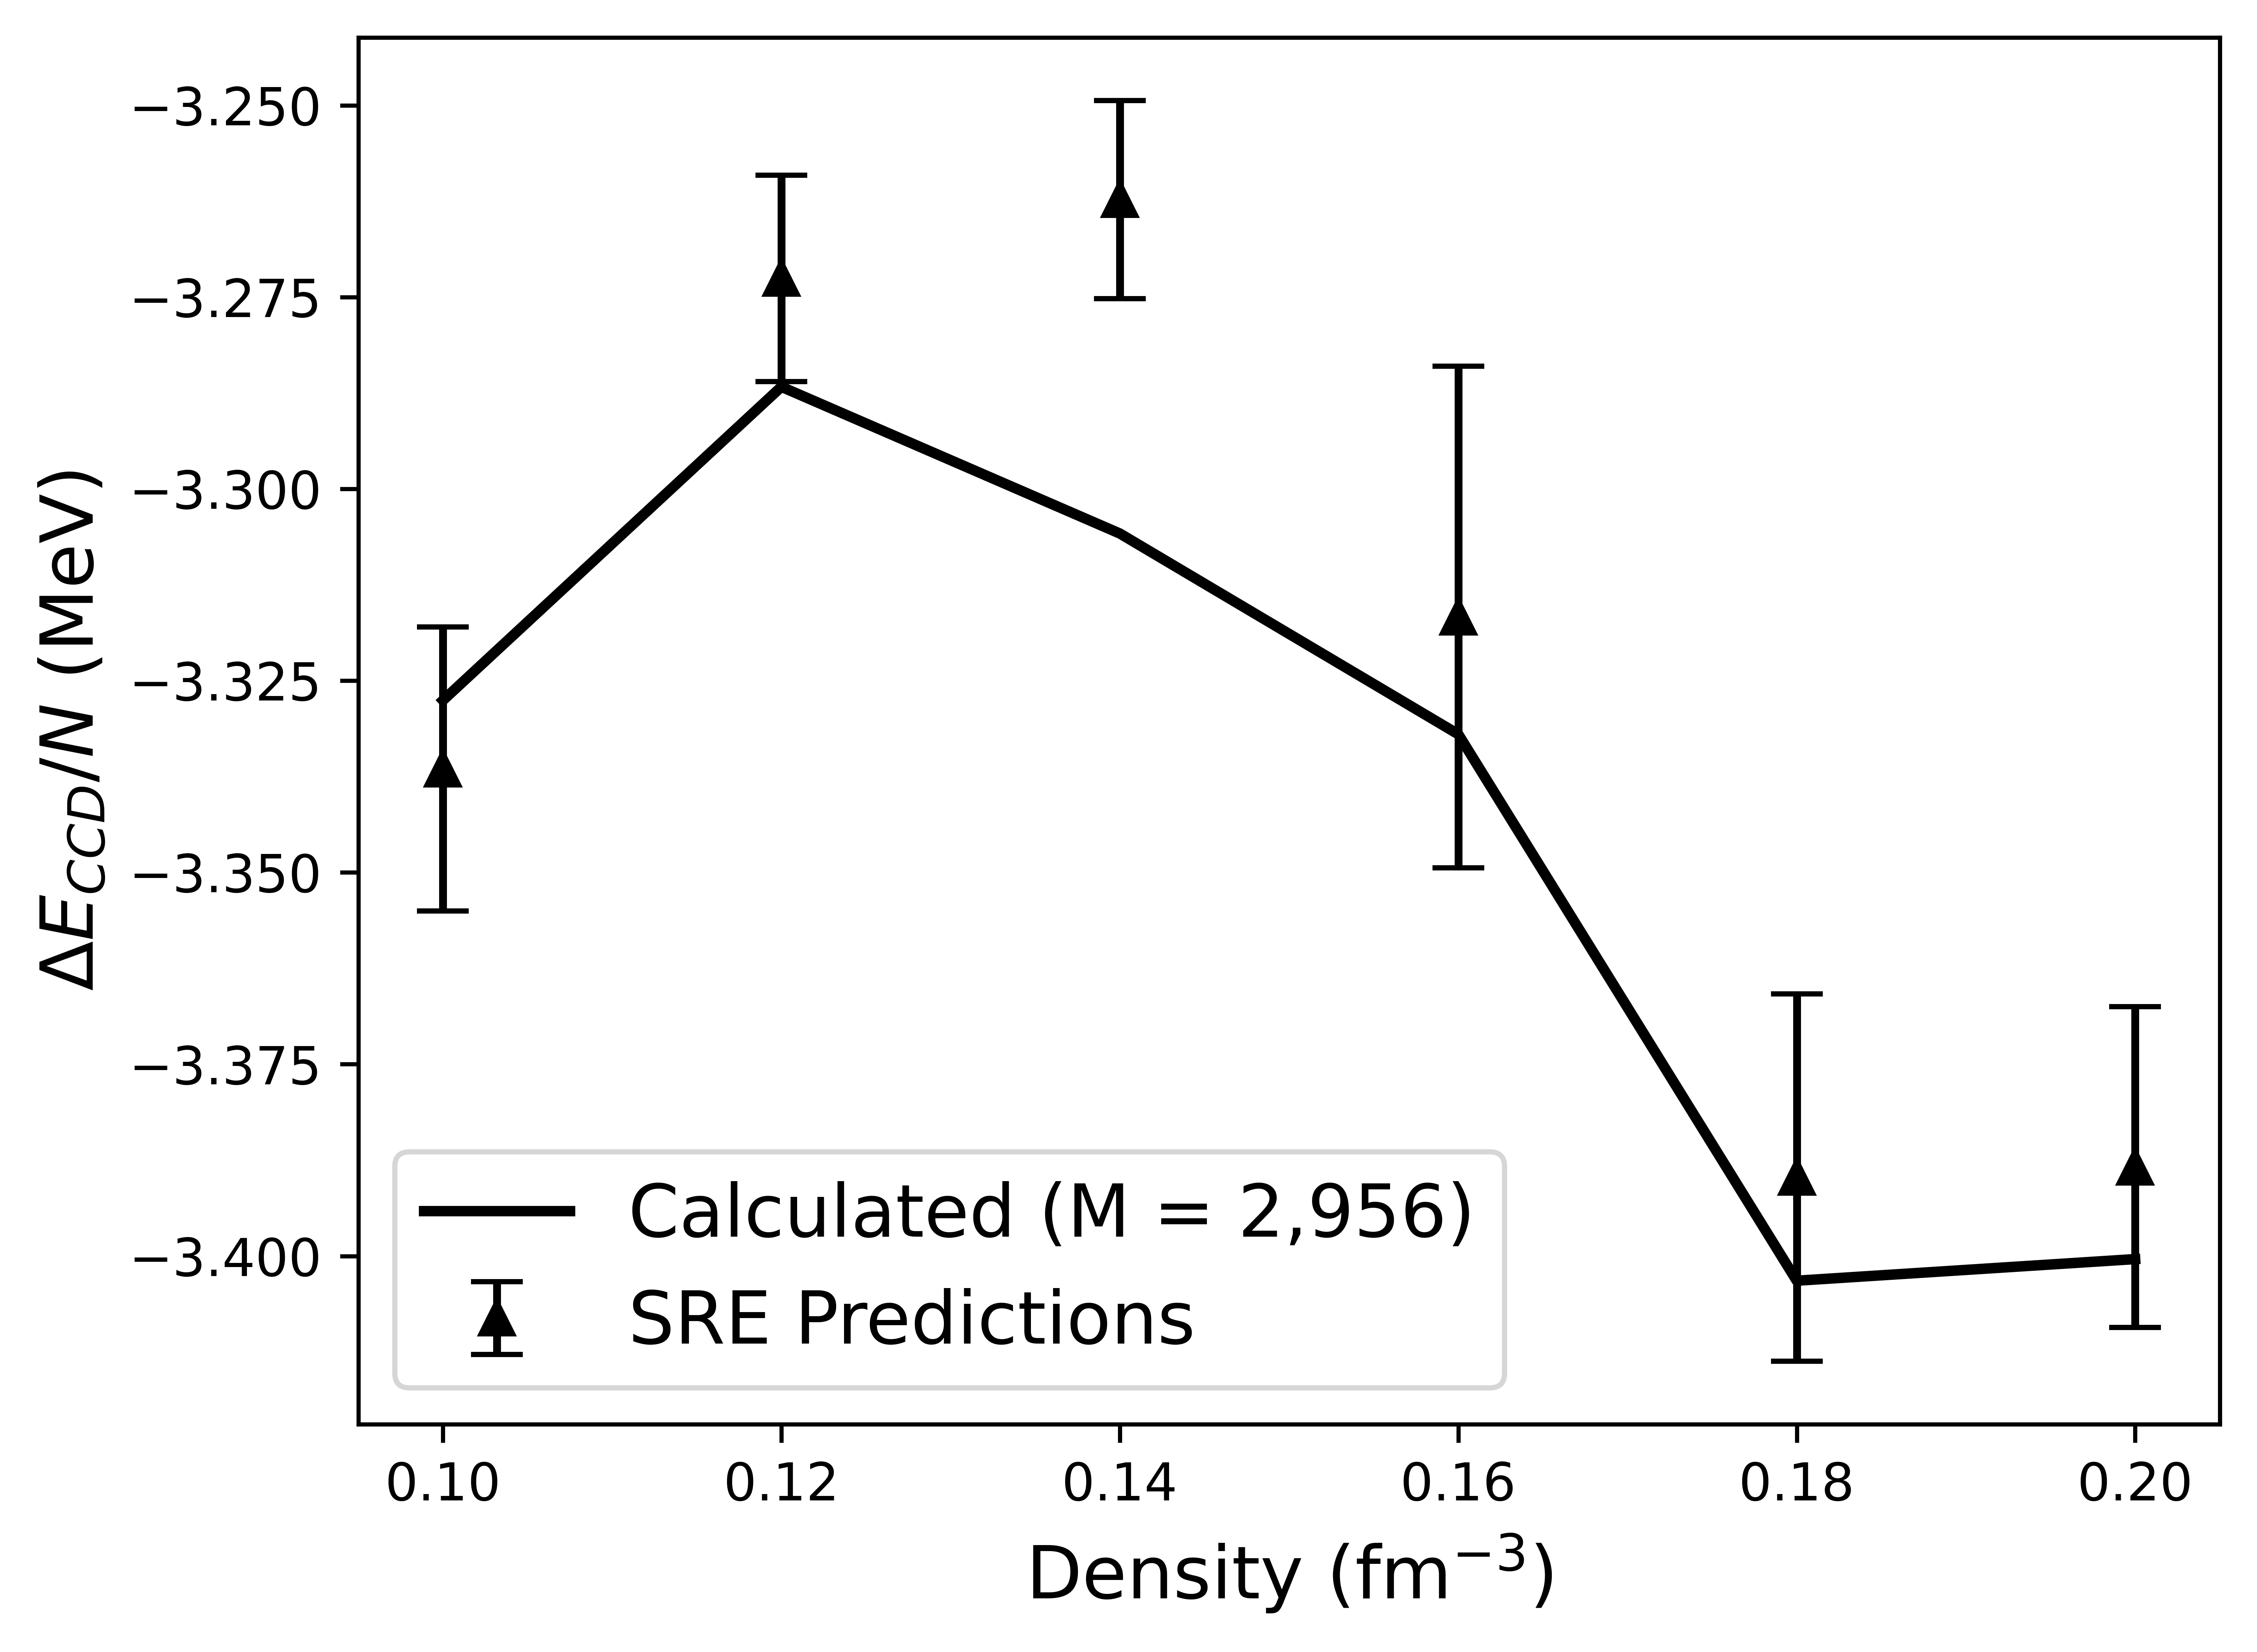
\includegraphics[scale=0.75]{Images/Chapter8/FinalReport3b-3.png}
    \caption{The CCD correlation energies for SNM calculated fully at M = 2,956 (solid line) and using the SRE method to predict them (triangular marker).  The average percent error of this graph is 0.54$\%$ and the time savings of using SRE over performing the full calculations is 6.48 node days.}
    \label{fig:snm_ccd}
\end{figure}

The SRE predictions in Fig. \ref{fig:snm_ccd} were generated using seven training points from M = 324 to M = 1,004. The SRE sequence length is used as three since there are more training data points here compared to the PNM case. In addition, the SNM CCD energy has a slower convergence than the PNM energies, leading to the use of more training data.

When predicting the CCD correlation energies using the SRE method, the average percent error between the predictions and the complete calculations at M = 2,956 is 0.54$\%$. This is compared to the average percent error between the calculations at M = 2,956 and M = 1,004 (the largest training data point) of 9.52$\%$. Thus the SRE provides a much more accurate method than truncating the calculations at the level of the training data. Furthermore, it takes 504.77 node hours to compute all six data points shown in Fig. \ref{fig:snm_ccd} at M = 2,956 but only 349.17 node hours to generate the training data needed by the SRE algorithm to predict all 6 points. This leads to a computational time savings of 155.61 node hours or 6.48 \textit{node days}. Thus the SRE method can accurately recreate the CCD correlation energies of an SNM system with significant time savings.
        \subsection{Coupled Cluster Doubles with Perturbative Triples and Realistic Potentials}

As a final data set with SRE, we will attempt to predict the converged correlation energies for SNM using the CCD(T) approximation.  The CCD(T) approximation has significantly higher time requirements than the CCD approximation, as we saw with the PNM case.  But this difference in time will be even higher more drastic for SNM since there will be a higher number of single-particle states. Remember that the expected computational time for a CCD calculation is $O(M^6)$, and for a CCD(T) calculation, it is $O(M^7)$.  This extra factor of M can contribute significantly to the run time since it can be as large as M = 2,956 for the fully converged calculations.  However, for this case, due to the high computational costs, we have truncated M to only 23 energy shells or M = 2,060.  At this level, the correlation energies have converged to an order of 10$^{-3}$ or less, so it should be sufficient for this work, but it is important to note that if the calculations were carried all the way out to M = 2,956 then the run times would be much higher.  We can see in Fig. \ref{fig:snm_ccdt_pert_times} that the CCD(T) run times (blue) are, in fact, much higher than the CCD run times.  The CCD(T) data was collected on Oak Ridge National Laboratory's Andes supercomputer using 3.0 GHz and 64 MPI nodes.  Since the CCD and CCD(T) data was collected on different supercomputers and with a different number of MPI nodes, in Fig. \ref{fig:snm_ccdt_pert_times}, we have standardized the run time by reporting it as node hour per GHz.

\begin{figure}
    \centering
    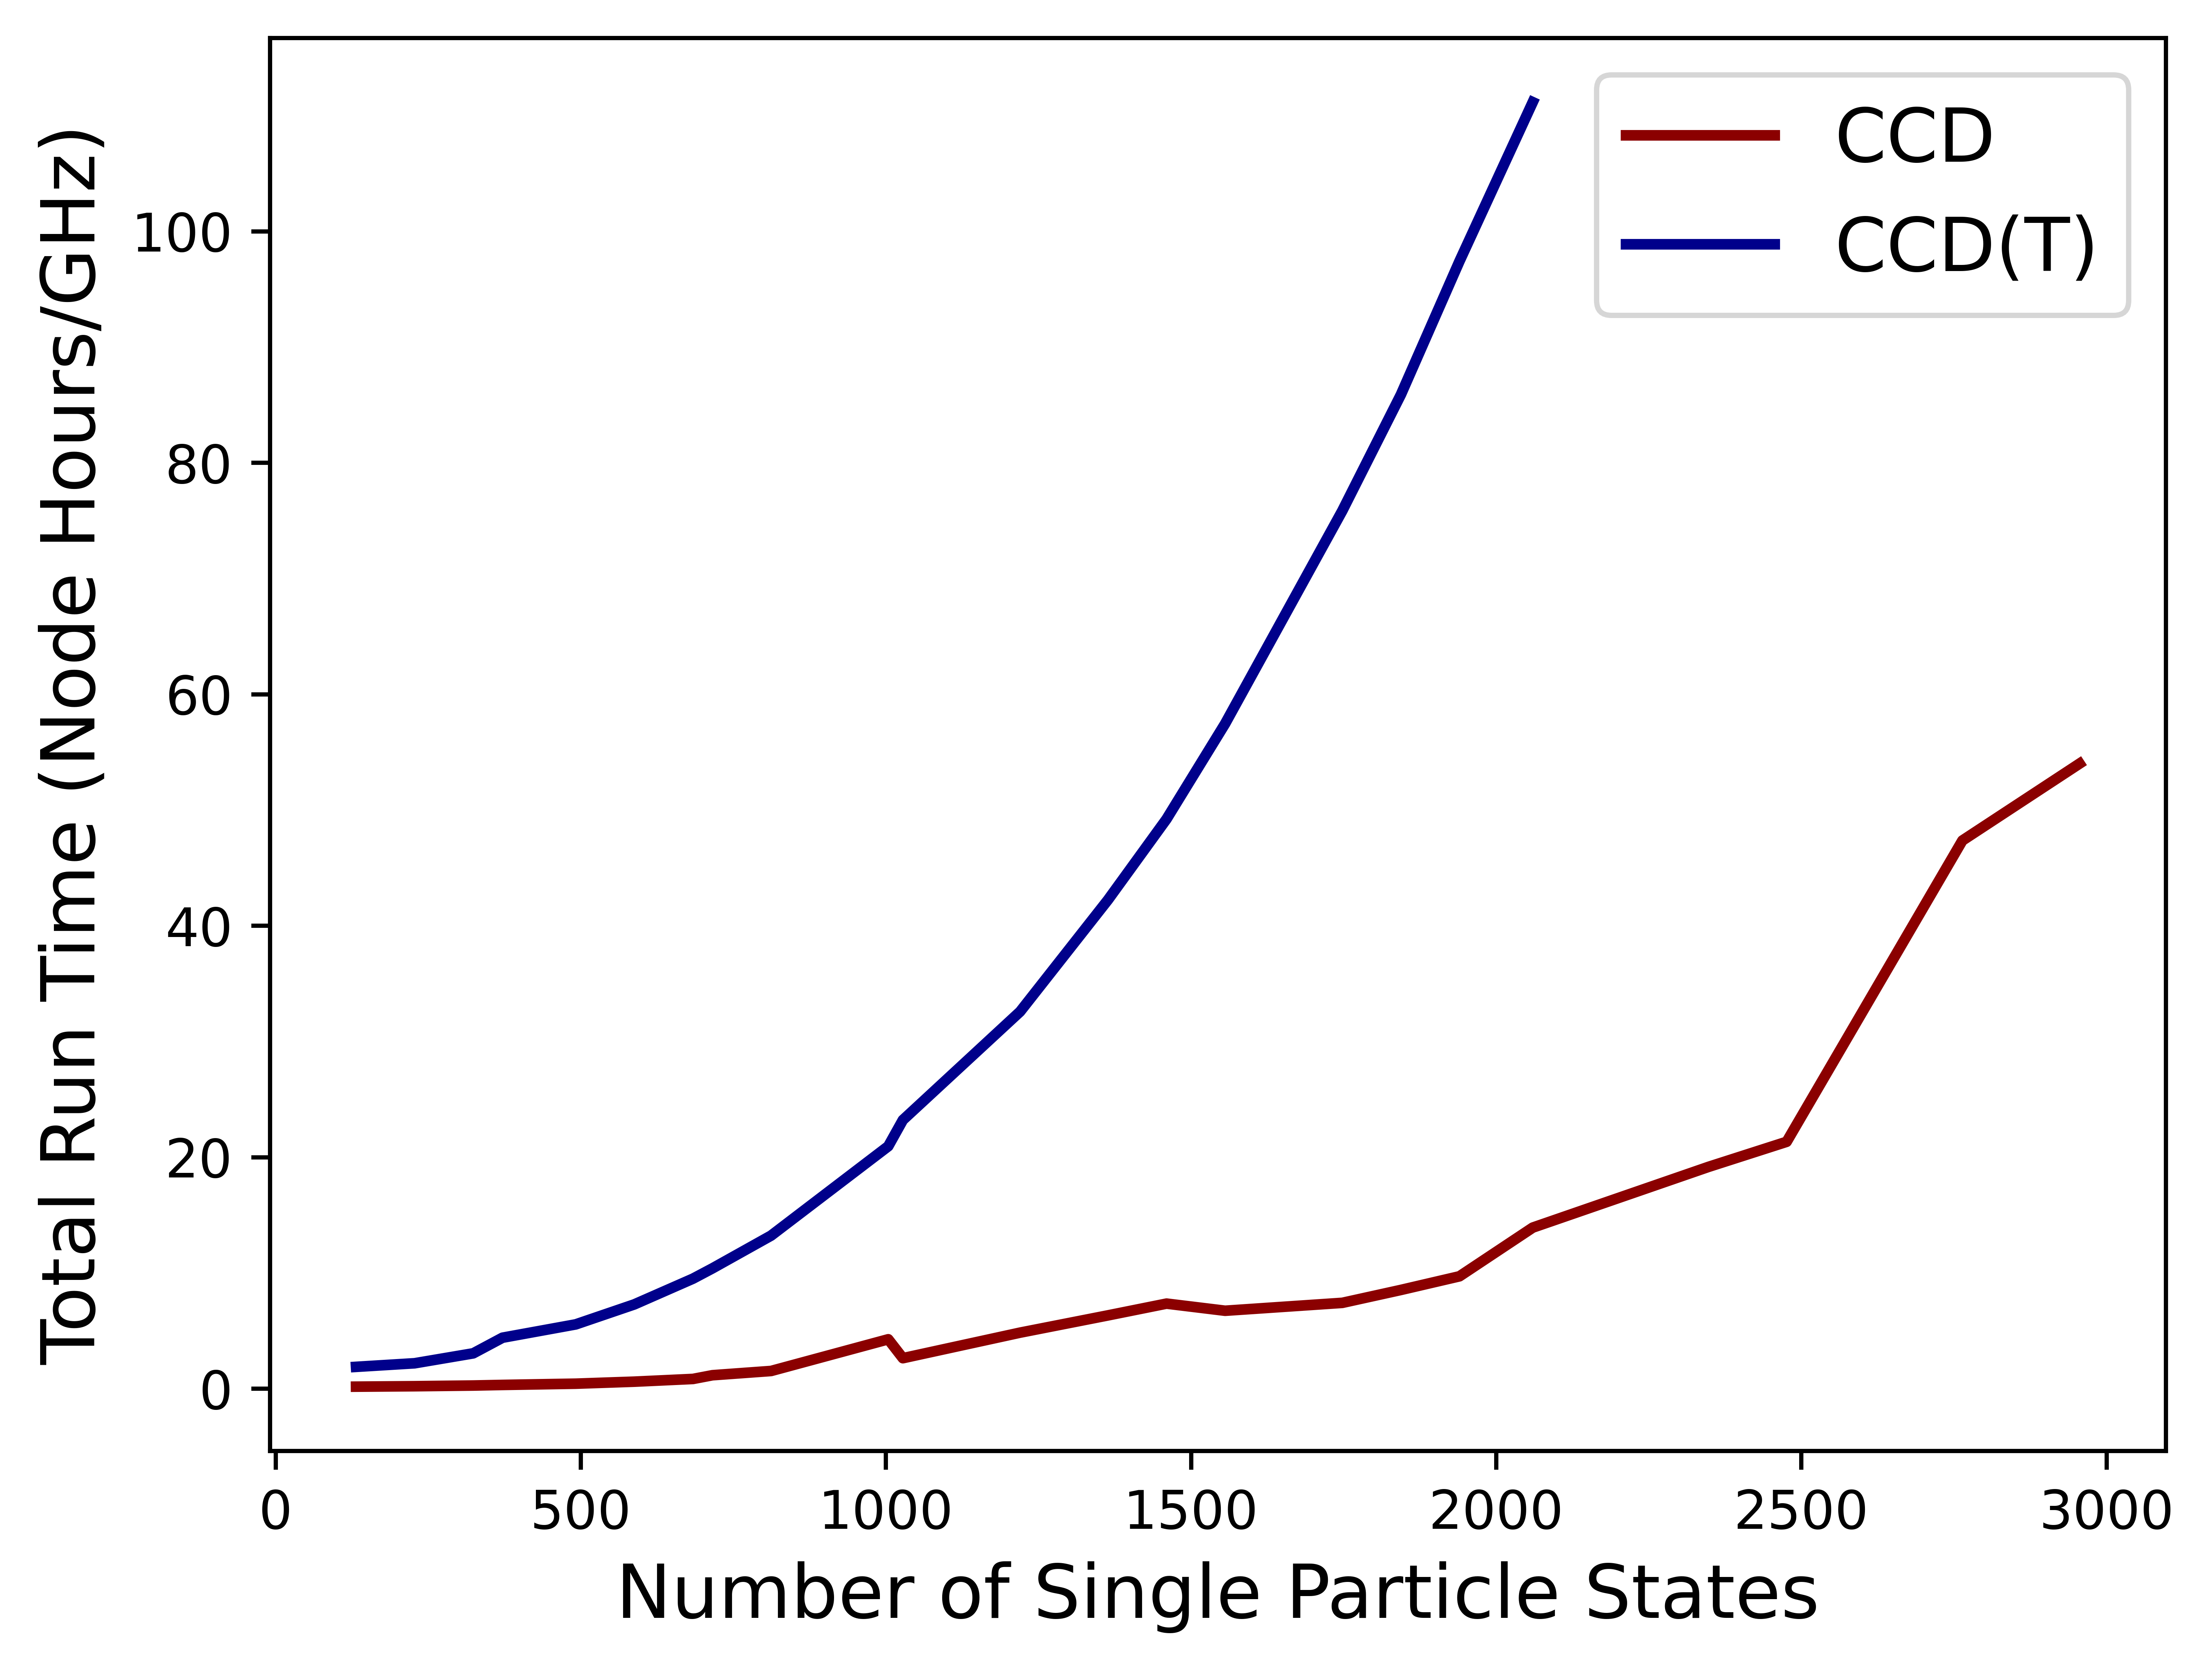
\includegraphics[scale=0.75]{Images/Chapter8/PRX_ORNL1_Fig2b.png}
    \caption{The run times (in node hours per GHz) for CCD calculations of SNM (red) and CCD(T) calculations of SNM (blue).  The CCD calculations were performed on processors which ran at 2.4GHz and used 24 MPI nodes, while the CCD(T) calculations were performed on processors that ran at 3.0GHz and used 64 MPI nodes.}
    \label{fig:snm_ccdt_pert_times}
\end{figure}

The average time to perform a CCD calculation of SNM at M = 2,956 is 84.12 node hours.  However, the average time to complete a CCD(T) calculation of SNM at only M = 2,060 is 335.65 node hours.  However, this significant increase in run time is necessary as the CCD(T) approximation adds some aspects of the $\hat{T}_3$ operator into the calculations neglected in the CCD approximation.  This does make the calculations more accurate (more comparable to an actual SNM system), but we do have to pay the much higher computational cost.  This further motivates the use of the SRE method because here we are taking almost 14 \textit{node days} per density of interest, making studies of, for example, the equation of state of nuclear matter prohibitively expensive.

Fig. \ref{fig:ccdt_pert_sre} shows the results of performing an SRE analysis on CCD(T) calculations of SNM.  The calculations at M = 2,060 are shown with the solid lines, and then SRE predictions are shown with triangular markers, which have error bars that come from the uncertainty of the Gaussian process algorithm; here, we have used six training points (from M = 162 to M = 406), and we have set the SRE sequence length to 1.  This results in an average percent error of 0.65$\%$.  Compared to the average percent error between the data at M = 406 (the largest training point) and the converged energies at M = 2,060 of 14.70$\%$, the SRE method accurately predicts the converged CCD(T) energies from unconverged energies.  Looking at the run times, it takes a total of 2,000.57 node hours to generate the six data points at M = 2,060, but it only takes 721.81 node hours to create the training data needed by the SRE algorithm, which is required to produce these converged correlation energies accurately.  This results in a time savings of 1,278.75 node hours or 53.28 \textit{node days}.

\begin{figure}
    \centering
    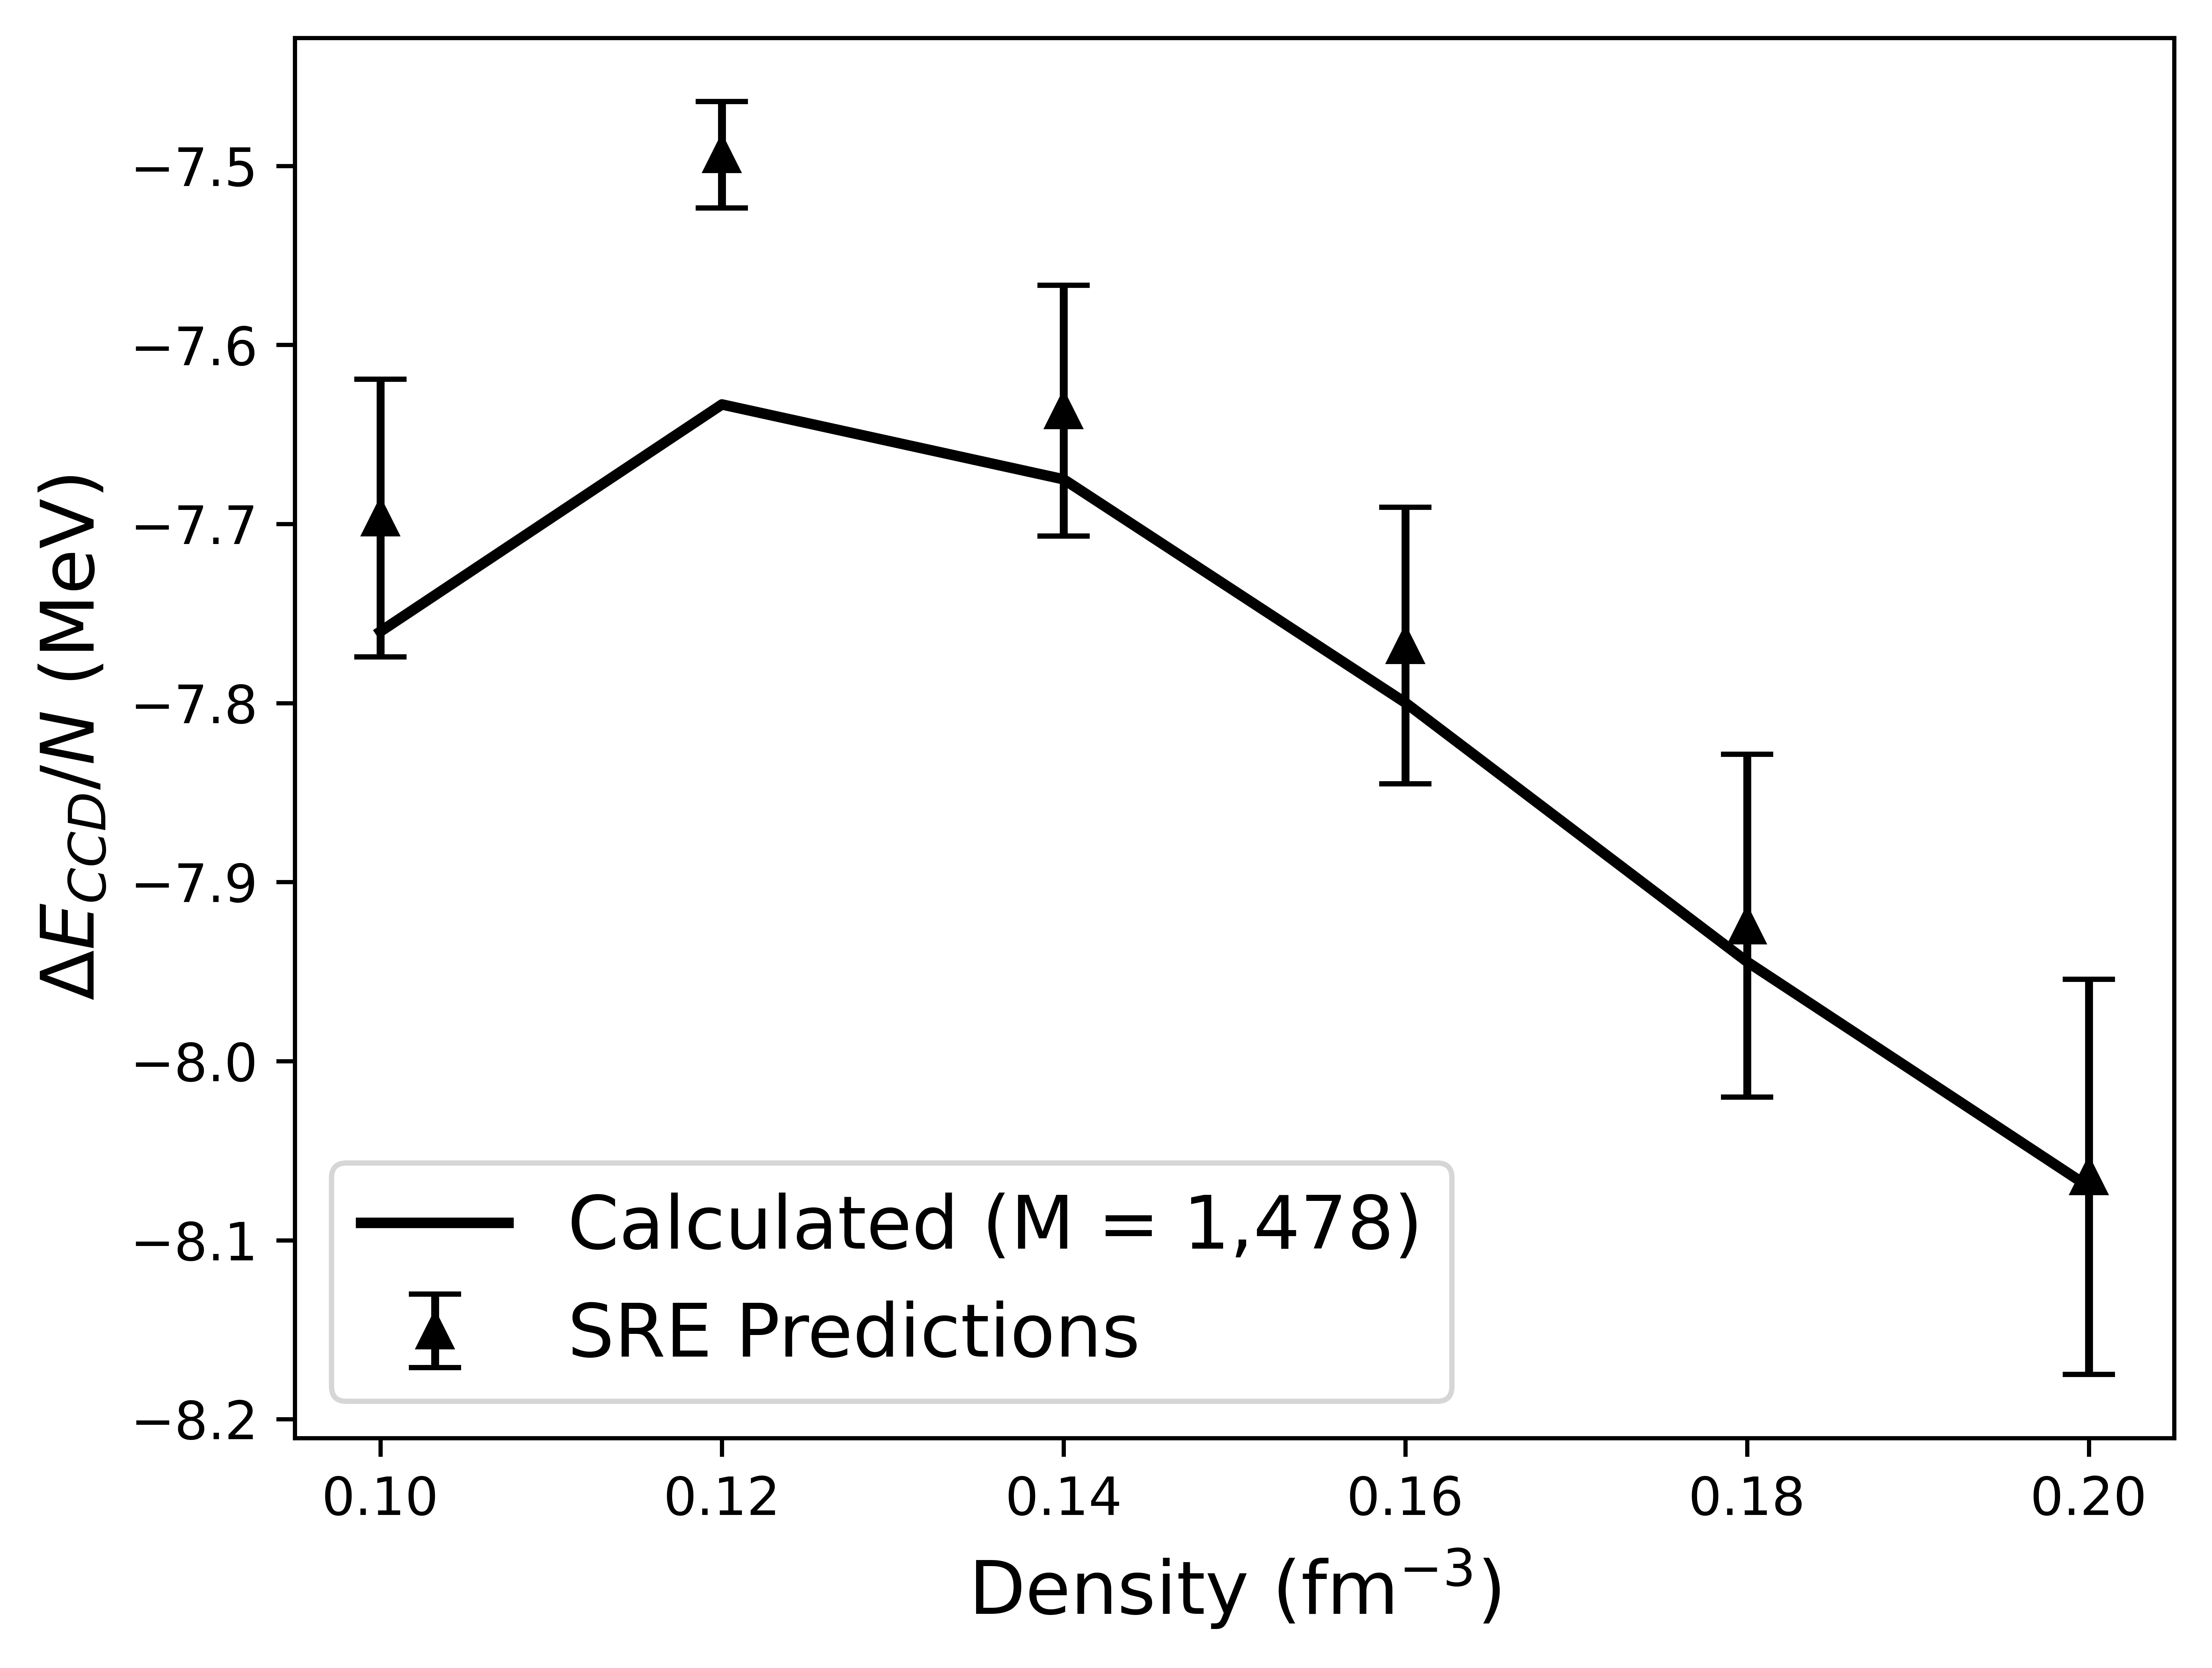
\includegraphics[scale=0.75]{Images/Chapter8/FinalReport4b.png}
    \caption{The CCD(T) correlation energies for SNM calculated at M = 2,060 (solid line) and predicted with SRE (triangular markers).}
    \label{fig:ccdt_pert_sre}
\end{figure}

Finally, we can compare the CCD correlation energies for SNM (red) and the CCD(T) correlation energies for SNM (blue) in Fig. \ref{ccd_ccdt_snm}. The complete calculations at M = 2,956 for CCD and M = 2,060 for CCD(T) are shown with solid lines, and the SRE markers are shown with triangular markers.  We draw two important conclusions from this figure.  First, the CCD and CCD(T) correlation energies are significantly different, so this does justify the higher computational cost of the CCD(T) calculations as the CCD(T) results should more closely model a real system as they take into account some aspects of the $\hat{T}_3$ operator.  Second, we can see that the SRE method performs well on both CCD and CCD(T) data sets, again showing that SRE works well on different coupled cluster data sets with no modifications of the algorithm besides changing the two hyperparameters: the number of training data points and the SRE sequence length.


\begin{figure}
    \centering
    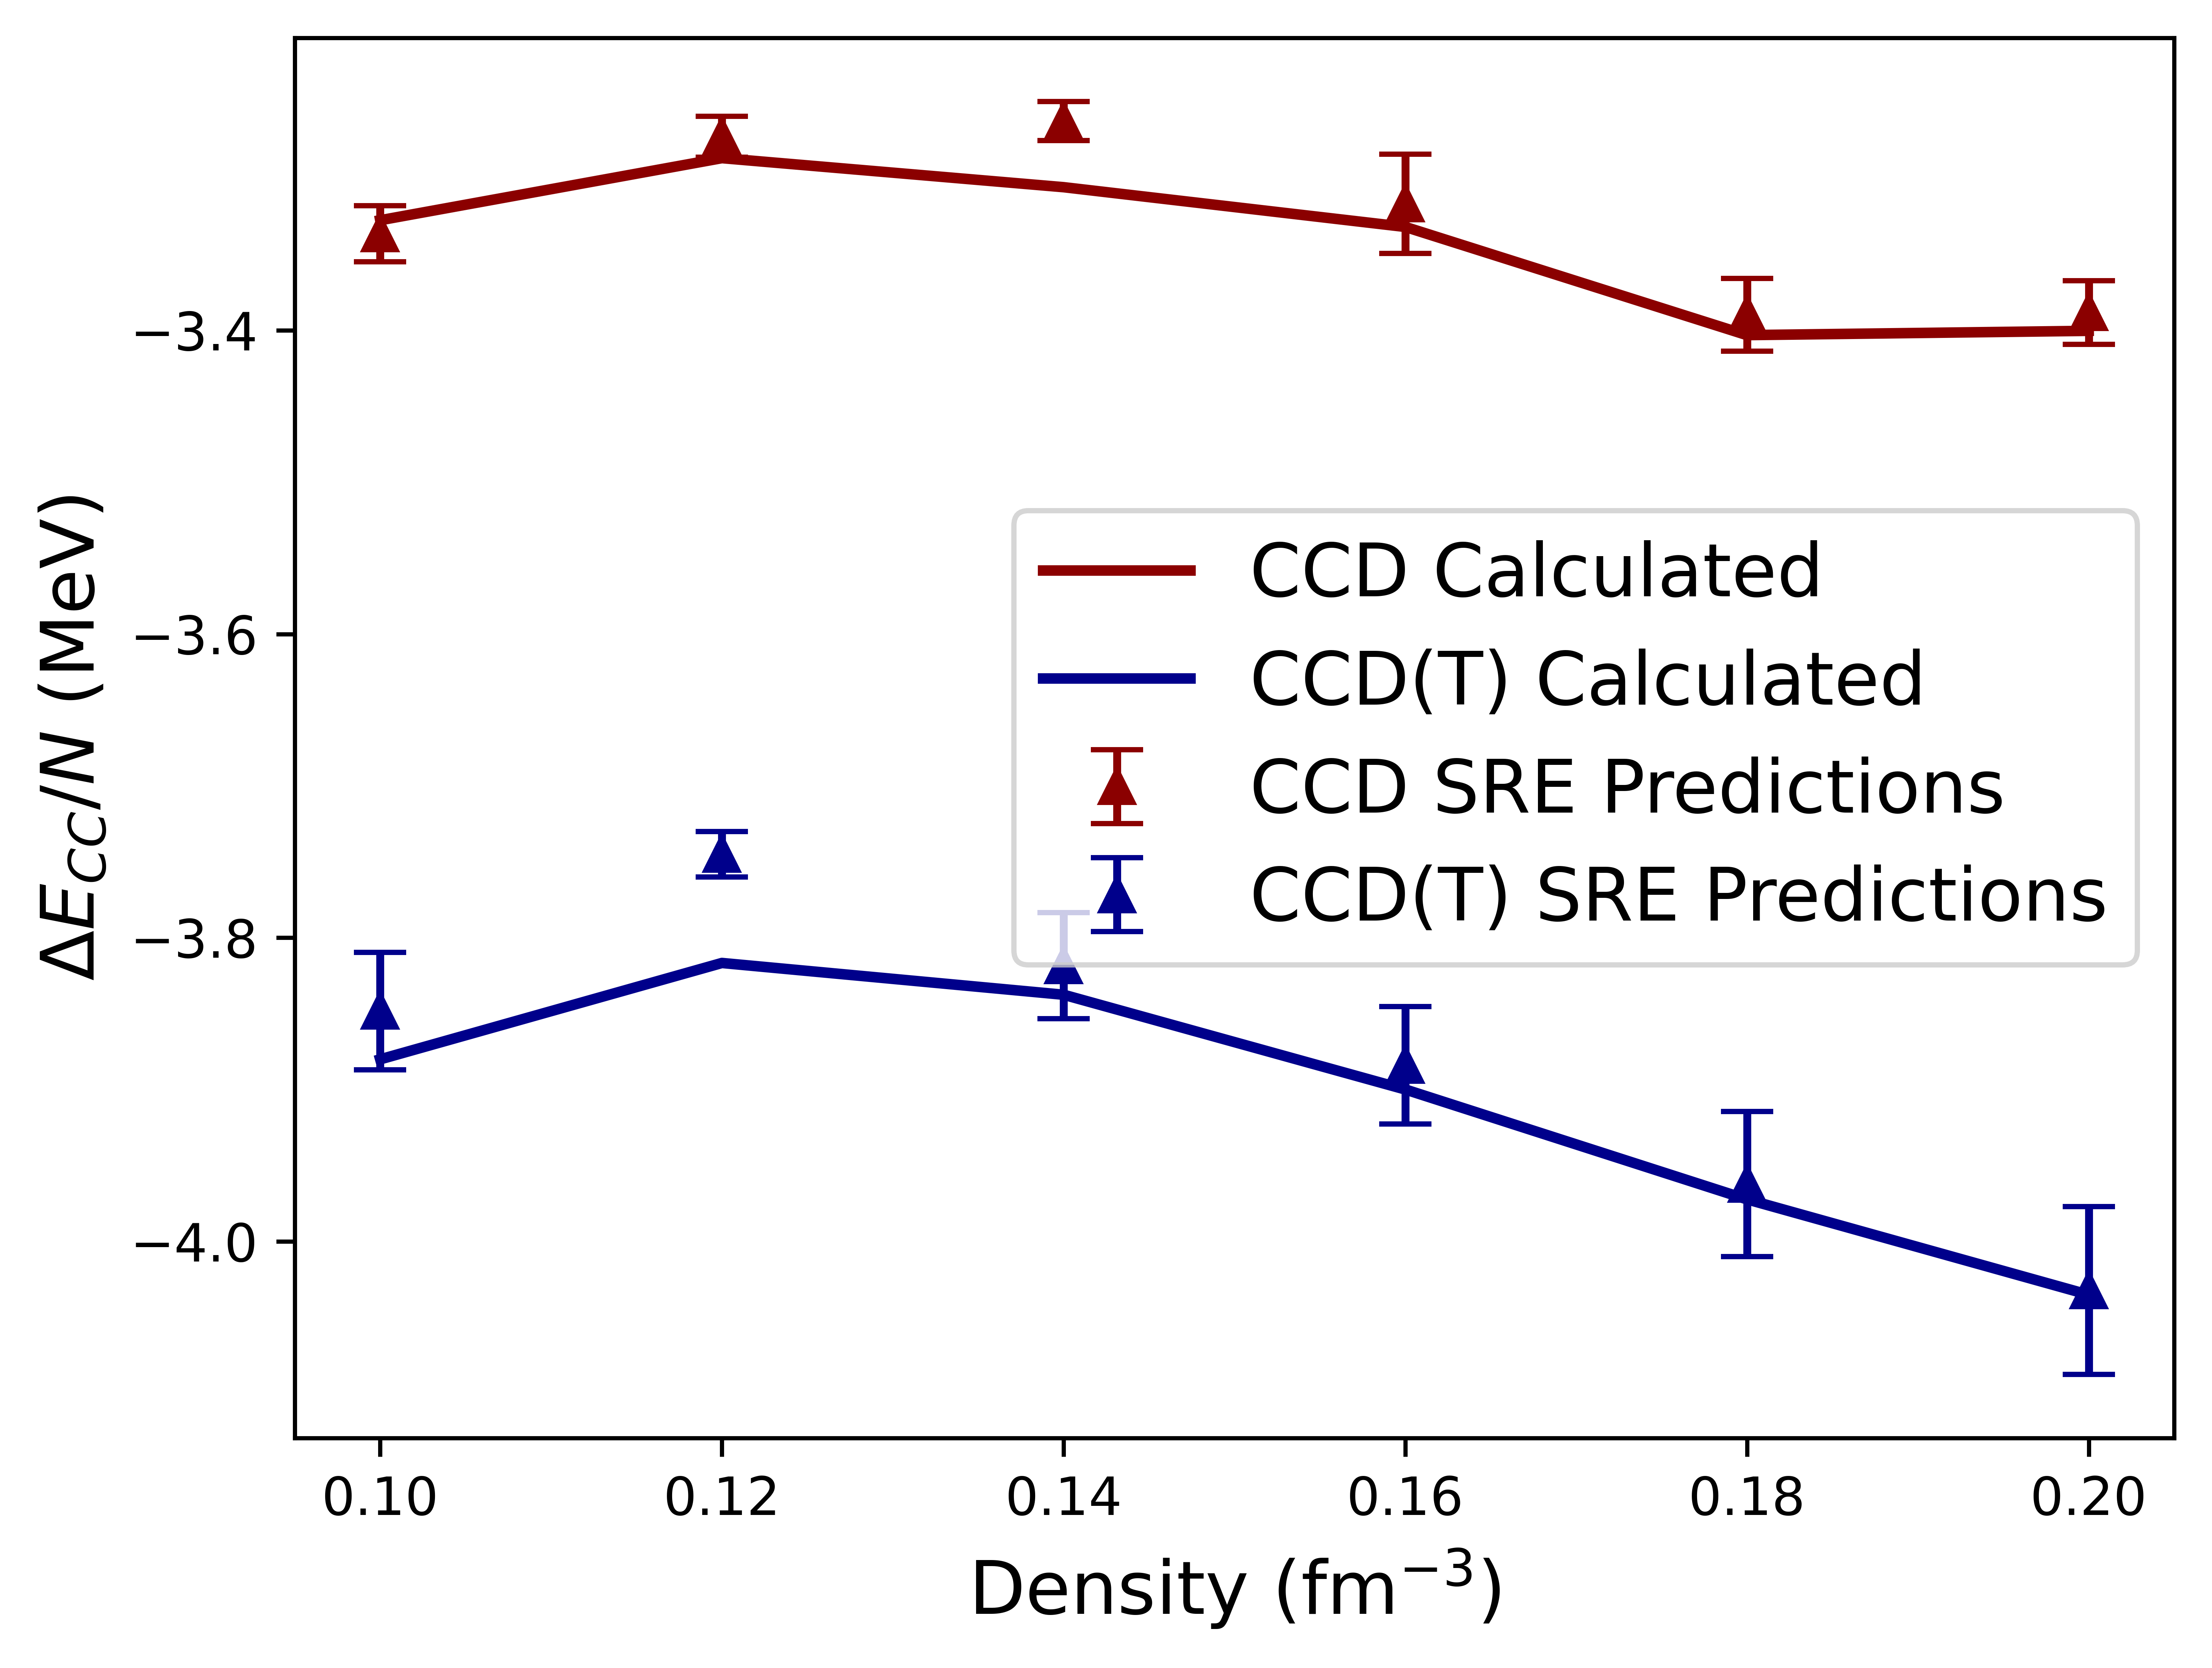
\includegraphics[scale=0.75]{Images/Chapter8/PRX_ORNL1_Fig3b.png}
    \caption{The correlation energies for SNM were calculated with CCD (red) and CCD(T) (blue).  The full calculations at M = 2,956 (CCD) and M = 2,060 (CCD(T)) are shown with solid lines, and the SRE predictions are shown with triangular markers.}
    \label{fig:ccd_ccdt_snm}
\end{figure}

    %%%%%%%%%%%%%%%%%%%%%%%%%%%%%%
    %% Symmetry Energy
    %%%%%%%%%%%%%%%%%%%%%%%%%%%%%%
    \section{Symmetry Energy}
        While we are limiting our infinite matter calculations only to pure neutron matter ($x_p = 0.0$) and symmetric nuclear matter ($x_p = 0.5$), we can still calculate a quantity that is important to studies of infinite nuclear matter and the nuclear equation of state. The quantity is the symmetry energy which is defined as:

    \begin{equation}
        \mathcal{l}(\rho) = E(\rho, x_p=0) - E(\rho, x_p=1/2).
    \end{equation}

Fig. \ref{fig:symmetry} shows the symmetry energies calculated for both the CCD approximation (red) and the CCD(T) approximation (blue) for densities around nuclear density. Additionally, the symmetry energies calculated with full converged energies at M = 1,478 for PNM and M = 2,956 for SNM are shown with the solid lines, and the symmetry energies calculated with SRE predictions are shown with triangular markers. Additionally, the uncertainty on the SRE predictions is shown with error bars. This uncertainty comes from the Gaussian process algorithm.  Note that this plot is energy per nucleon instead of correlation energy per nucleon as the other plots in this chapter.

\begin{figure}
    \centering
    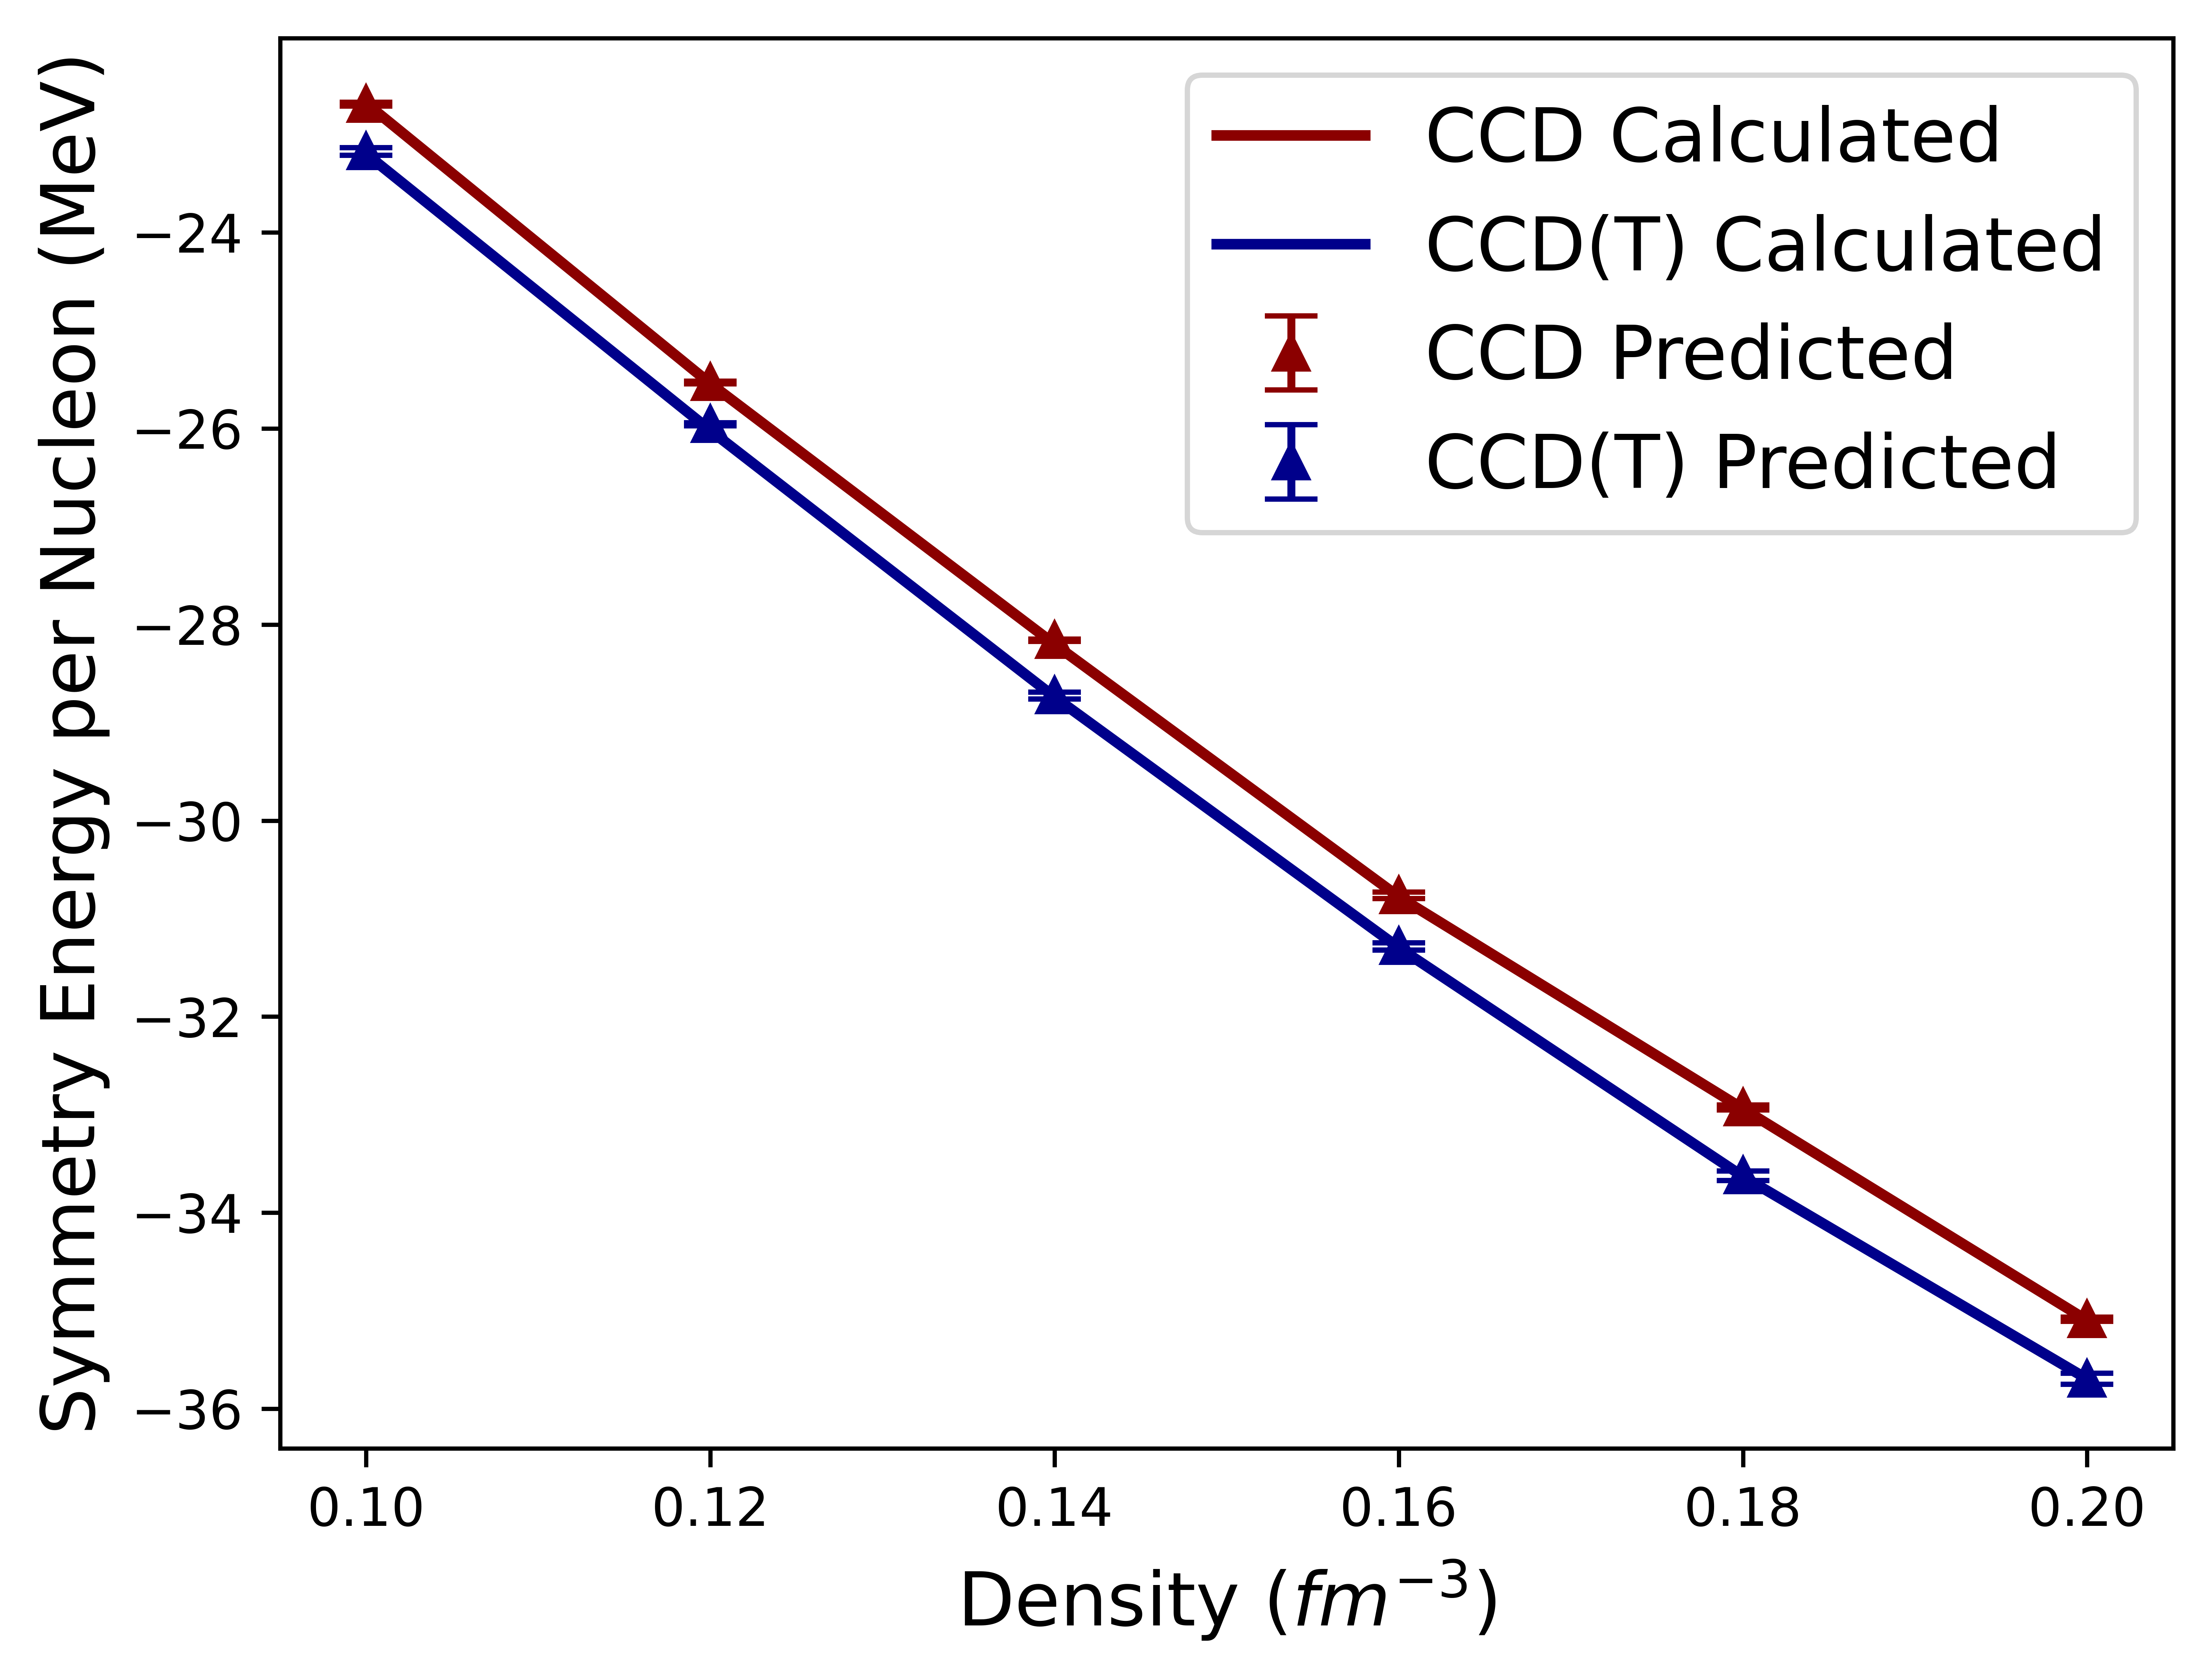
\includegraphics[scale=0.75]{Images/Chapter8/symmetryenergy.png}
    \caption{The symmetry energy for infinite nuclear matter is calculated using the CCD approximation (red) and the CCD(T) approximation (blue). The symmetry energy calculated from fully converged calculations is shown with the solid lines and SRE predictions with the triangular points. Error bars also represent the uncertainty on the symmetry energy from SRE predictions from the Gaussian process algorithm.}
    \label{fig:symmetry}
\end{figure}

For the CCD approximation, the average percent error between the two data sets is 0.056$\%$, and for the CCD(T) approximation, it is 0.078$\%$. Note that these percent errors are much smaller than previous results because we are considering the total energy instead of just the correlation energies so small differences have much less of an impact. We also need to consider time savings as a justification for performing the SRE method over the complete calculations for the symmetry energy. The time needed to generate all 12 points (6 for PNM and 6 for SNM) needed to calculate the symmetry energy at M = 1,478, or 2,956, is 661.22 node hours for the CCD approximation and 2608.11 node hours for the CCD(T) approximation. The time needed to generate all training data for the CCD approximation is 353.05 node hours and 1472.10 node hours for the CCD(T) approximation. The training data requires just 55.8$\%$ of the computational time it takes to generate the fully converged energies and most of this time is due to the high cost of SNM calculations. This leads to a time savings of 20.11 \textit{node days} for the CCD approximation with an average error of 0.056$\%$. The time savings for the CCD(T) approximation is 47.33 \textit{node days} with an average percent error of only 0.078$\%$. Therefore, when calculating the symmetry energy, the SRE method provides an accurate prediction and can save many days of computational time.

    %%%%%%%%%%%%%%%%%%%%%%%%%%%%%%
    %% Conclusion
    %%%%%%%%%%%%%%%%%%%%%%%%%%%%%%
    \section{Final Remarks}
        As pointed out in the pure neutron matter section of this chapter, the main goal of this chapter is not to compare coupled cluster calculations with different levels of approximation, different nuclear interactions, and different infinite nuclear matter systems. Though we have made some of these comparisons, the main point of this chapter is to analyze the accuracy and time savings of the SRE algorithm. As we have seen throughout this chapter, coupled cluster calculations of nuclear systems have very large (and possibly prohibitive) computational times, especially when using realistic nuclear interactions and higher-order coupled cluster approximations. The SRE method, with its ability to make accurate extrapolations with a small amount of training data, can make these studies more feasible by drastically reducing the run times needed to perform the calculations. This is especially important when we realize that studies of the nuclear equation of state (an essential future work for this thesis) will require accurate calculations at different densities and proton fractions. Thus, the development of the SRE method, by reducing the computational time needed to perform accurate calculations, makes large-scale studies of infinite nuclear matter much more feasible, paving the way for novel studies to occur in the future.
    


%%%%%%%%%%%%%%%%%%%%%%%%%%%%%%
%% CHAPTER: CONCLUSION
%%%%%%%%%%%%%%%%%%%%%%%%%%%%%%
\chapter{Conclusion}
    %%% THESIS CONCLUSIONS %%%

% SRE as a valid extrapolation method
The sequential regression extrapolation (SRE) method developed here based on Bayesian regression algorithms is an accurate and valuable extrapolator for removing basis incompleteness errors from coupled cluster calculations of infinite matter systems. Furthermore, when the infinite matter system needs to be taken to the thermodynamic limit, it is possible to use SRE to perform this task. Since the SRE algorithm uses training data taken from calculations at small numbers of single-particle states to predict the correlation energy at many single-particle states, the SRE algorithm can offer significant time savings over performing fully converged correlation energy calculations. As shown in this thesis, using the SRE algorithm to save over 100 node hours in the calculations of just one correlation energy is possible. Furthermore, this huge time savings does come with a loss in the accuracy of performing the whole savings. However, the average percent error between the SRE prediction and the fully calculated result was typically less than 1$\%$, making it quite a slight difference compared to the large amount of computational time that has been saved.

% From the CCD vs. CCDT side
Furthermore, besides developing the SRE method, we also compared different methods of performing coupled cluster calculations of systems of infinite nuclear matter. First, we compared the results from two different interactions: the Minnesota potential, a toy interaction, and chiral NNLO potentials, which are much more realistic. By comparing these two, we learned that they differ quite significantly around densities of infinite nuclear matter that are similar to nuclear densities and that calculations containing NNLO potentials do take much longer to compute compared to a Minnesota potential applied to the same system. Furthermore, we could also compare the difference between the coupled cluster approximations CCD, CCDT-1, and CCD(T) on calculations of infinite matter systems. We found that the triples approximations give significant results when compared to the CCD approximation, so they are worth performing even though they provide an increase in computational time.

%% SIZE OF MACHINE LEARNING SYSTEM
Though it has been mentioned throughout this thesis, it is essential to emphasize the size of the training data sets used in this work. This work's most extensive training data set used only 16 training points, and the smallest training set used only 3 points. Some areas of physics could be faster to adopt machine learning because of the vast amount of training data that some machine learning algorithms require. However, this work has shown that accurate machine learning predictions can be made with very few training points, thus encouraging using machine learning as a tool in fields with small data sets.

%%% FUTURE WORKS %%%

\subsection*{Possible Future Works}
% Full triples and different proton fractions
A few notable future works stem directly from the work presented here. First, while we showed results from both the CCD< CCDT-1, and CCD(T) approximations, we did not have the capabilities to produce coupled cluster correlation energies using a complete CCDT calculation. This is mainly due to the high computational costs of a complete triple calculation ($O(M^8)$), but advancements, such as those made in Refs. Furthermore, ADD REFERENCES HERE are making this a much more achievable goal for the near future.

Additionally, while we only looked at pure neutron matter and symmetric nuclear matter here, there are other proton fractions of interest. If we want to model the equation of the state of nuclear matter thoroughly, then we need to be able to accurately predict the properties of neutron matter at proton fractions beyond just 0.0 and 0.5.

% PARAGRAPH ABOUT NOT BEING LIMITED TO INFINITE SYSTEMS
While truncating the number of particles in a calculation is limited to infinite matter and other large systems, truncations occur in every \textit{ab initio} many-body calculation. Basis truncation is especially common and occurs in almost every calculation except some simple toy models. The last part of this thesis will be dedicated to exploring some possible future applications of the SRE methodology which has been developed.

% PARAGRAPH ABOUT CC CALCULATIONS OF THE NUCLEUS
An extension of the work presented in this thesis is to apply the SRE method to remove basis incompleteness errors from coupled cluster calculations of nuclei. Though nuclei are finite systems and the number of nucleons in the system generally does not need to be truncated, the number of single-particle states is still truncated, leading to a need to extrapolate to an infinite model space \cite{Ref6}. This is especially true for heavy nuclei and nuclei that are weakly bound \cite{Ref6}. There are methods to perform these extrapolations on nuclei calculations, but when using the harmonic oscillator basis, which mixes the ultraviolet and infrared cutoffs, these extrapolation methods can fail \cite{Ref6}. Machine learning has been used to perform similar extrapolations (see Ref. \cite{Ref6}, \cite{Ref22}, \cite{Ref23}, for example), but these were performed with neural networks and thus incurred all of the problems that were experienced with neural networks in this thesis.

%% MBPT CALCULATIONS AND HIGHER ORDERS
Additionally, the SRE method has no reason to be restricted to only predicting CC energies using MBPT2 energies. Extending the SRE method to other many-body methods should also be possible. 

% PARAGRAPH ABOUT FCI
One of the most accurate yet restricted \textit{ab initio} many-body methods is full configuration interaction theory (FCI), which uses a variationally optimized linear combination of the full set of Slater determinants. FCI is used in nuclear physics and electronic-structure theory, but its complexity limits it to only the smallest of systems. The ground state energy, which FCI finds, is the lowest (variationally) and most accurate that can be achieved. If an infinite single particle basis is used, FCI produces the solutions to the Schr\"{o}dinger equation. However, due to computational limitations, FCI calculations must be performed with a finite basis, meaning they will fail to retrieve the total energy \cite{Ref1}. However, it is possible that SRE could be applied to FCI calculations using, for example, Hartree Fock calculations as the "fast method" to quickly and accurately extrapolate FCI results to the infinite basis limit, thus recovering the Schr\"{o}dinger equation results.

 % APPLICATIONS OUTSIDE OF NUCLEAR PHYSICS
While most of this thesis, except for the sections on the electron gas, have been devoted to nuclear physics applications, \textit{ab initio} many-body methods occur in many other fields besides nuclear physics. For example, coupled cluster theory, and other many-body methods, are prevalent in other fields of physics and quantum chemistry. Therefore, the development of the SRE method should improve calculations outside of the realm in which it was developed.

%%%%%%%%%%%%%%%%%%%%%%%%%%%%%%
%% CHAPTER: REFERENCES
%%%%%%%%%%%%%%%%%%%%%%%%%%%%%%
%\bibliography{bib}
\printbibliography

\end{document}
\fi
